\documentclass[12pt,a4paper]{book}
\usepackage[utf8]{inputenc}
\usepackage[russian]{babel}
\usepackage{amsmath}
\usepackage{amsfonts}
\usepackage{amssymb}
\usepackage{graphicx}

\title{\textbf{Повесть о Ходже Насреддине} \\ Возмутитель спокойствия}
\author{Леонид Соловьёв}
\date{1940~г. \\ Рисунки художника С.~Забалуева \\ (изд-во «Молодая гвардия», 1958~г.) \\ Вёрстка --- m1kc, 2012~г.}

\begin{document}

\maketitle

Памяти моего незабвенного друга Мумина Адилова, погибшего 18 апреля 1930 года в горном кишлаке Нанай от~подлой вражеской пули, посвящаю, благоговея перед его чистой памятью, эту книгу.

В~нем были многие и~многие черты Ходжи Насреддина~— беззаветная любовь к~народу, смелость, честное лукавство и~благородная хитрость,~— и~когда я~писал эту книгу, не~один раз мне казалось в~ночной тишине, что его тень стоит за~моим креслом и~направляет мое перо.

Он~похоронен в~Канибадаме. Я~посетил недавно его могилу; дети играли вокруг холма, поросшего весенней травой и~цветами, а~он~спал вечным сном и~не~ответил на~призывы моего сердца...

\begin{quote}
И~сказал ему~я: «Для радости тех, что живут со~мною на~земле, я~напишу книгу,~— пусть на~ее~листы не~дуют холодные ветры времени, пусть светлая весна моих стихов никогда не~сменяется унылой осенью забвенья!..» И~— посмотри! —~еще розы в~саду не~осыпались, и~я~еще хожу без клюки, а~книга «Гюлистан», что значит «Цветник роз», уже написана мною, и~ты~читаешь~ее...
\flushright{\textit{Саади}}
\end{quote}

\begin{quote}
Эту историю передал нам Абу-Омар-Ахмед-ибн-Мухаммед со слов Мухаммеда-ибн-Али-Рифаа, ссылавшегося на~Али-ибн-Абд-аль-Азиза, который ссылался на~Абу-Убейда-аль-Хасима-ибн-Селяма, говорившего со~слов своих наставников, а~последний из~них опирается на~Омара-ибн-аль-Хаттаба и~сына его Абд-Аллаха,~— да~будет доволен аллах ими обоими!
\flushright{\textit{Ибн-Хазм, «Ожерелье голубки»}}
\end{quote}

\begin{figure}[p]
\centering

\includegraphics[scale=0.8]{1.png}
\end{figure}

\part{}

\begin{quote}
Рассказывают также, что один простак шел, держа в~руке узду своего осла, которого он~вел за~собою.
\flushright{\textit{Триста восемьдесят восьмая ночь Шахразады}}
\end{quote}

\chapter{}

Тридцать пятый год своей жизни Ходжа Насреддин встретил в~пути.

Больше десяти лет провел он~в~изгнании, странствуя из~города в~город, из~одной страны в~другую, пересекая моря и~пустыни, ночуя как придется~— на~голой земле у~скудного пастушеского костра, или в~тесном караван-сарае, где в~пыльной темноте до~утра вздыхают и~чешутся верблюды и~глухо позвякивают бубенцами, или в~чадной, закопченной чайхане, среди лежащих вповалку водоносов, нищих, погонщиков и~прочего бедного люда, с~наступлением рассвета наполняющего своими пронзительными криками базарные площади и~узкие улички городов. Нередко удавалось ему ночевать и~на~мягких шелковых подушках в~гареме какого-нибудь иранского вельможи, который как раз в~эту ночь ходил с~отрядом стражников по~всем чайханам и~караван-сараям, разыскивая бродягу и~богохульника Ходжу Насреддина, чтобы посадить его на~кол... Через решетку окна виднелась узкая полоска неба, бледнели звезды, предутренний ветерок легко и~нежно шумел по~листве, на~подоконнике начинали ворковать и~чистить перья веселые горлинки. И~Ходжа Насреддин, целуя утомленную красавицу, говорил:

—~Пора. Прощай, моя несравненная жемчужина, и~не~забывай меня.

—~Подожди! —~отвечала она, смыкая прекрасные руки на~его шее. —~Разве ты~уходишь совсем? Но~почему? Послушай, сегодня вечером, когда стемнеет, я~опять пришлю за~тобой старуху. —~Нет. Я~уже давно забыл то~время, когда проводил две ночи подряд под одной крышей. Надо ехать, я~очень спешу.

—~Ехать? Разве у~тебя есть какие-нибудь неотложные дела в~другом городе? Куда ты~собираешься ехать?

—~Не~знаю. Но~уже светает, уже открылись городские ворота и~двинулись в~путь первые караваны. Ты~слышишь~— звенят бубенцы верблюдов! Когда до~меня доносится этот звук, то~словно джины вселяются в~мои ноги, и~я~не~могу усидеть на~месте!

—~Уходи, если так! —~сердито говорила красавица, тщетно пытаясь скрыть слезы, блестевшие на~ее~длинных ресницах. —~Но~скажи мне хоть свое имя на~прощание.

—~Ты~хочешь знать мое имя? Слушай, ты~провела ночь с~Ходжой Насреддином! Я~— Ходжа Насреддин, возмутитель спокойствия и~сеятель раздоров, тот самый, о~котором ежедневно кричат глашатаи на~всех площадях и~базарах, обещая большую награду за~его голову. Вчера обещали три тысячи туманов, и~я~подумал даже~— не~продать~ли мне самому свою собственную голову за~такую хорошую цену. Ты~смеешься, моя звездочка, ну, дай мне скорее в~последний раз твои губы. Если~бы я~мог, то~подарил~бы тебе изумруд, но~у~меня нет изумруда,~— возьми вот этот простой белый камешек на~память!

Он~натягивал свой рваный халат, прожженный во~многих местах искрами дорожных костров, и~удалялся потихоньку. За~дверью громко храпел ленивый, глупый евнух в~чалме и~мягких туфлях с~загнутыми кверху носами~— нерадивый страж главного во~дворце сокровища, доверенного ему. Дальше, врастяжку на~коврах и~кошмах, храпели стражники, положив головы на~свои обнаженные ятаганы. Ходжа Насреддин прокрадывался на~цыпочках мимо, и~всегда благополучно, словно~бы становился на~это время невидимым.

И~опять звенела, дымилась белая каменистая дорога под бойкими копытами его ишака. Над миром в~синем небе сияло солнце; Ходжа Насреддин мог не~щурясь смотреть на~него. Росистые поля и~бесплодные пустыни, где белеют полузанесенные песком верблюжьи кости, зеленые сады и~пенистые реки, хмурые горы и~зеленые пастбища, слышали песню Ходжи Насреддина. Он~уезжал все дальше и~дальше, не~оглядываясь назад, не~жалея об~оставленном и~не~опасаясь того, что ждет впереди.

А~в~покинутом городе навсегда оставалась жить память о~нем.

Вельможи и~муллы бледнели от~ярости, слыша его имя; водоносы, погонщики, ткачи, медники и~седельники, собираясь по~вечерам в~чайханах, рассказывали друг другу смешные истории о~его приключениях, из~которых он~всегда выходил победителем; томная красавица в~гареме часто смотрела на~белый камешек и~прятала его в~перламутровый ларчик, услышав шаги своего господина.

—~Уф! —~говорил толстый вельможа~и, пыхтя и~сопя, начинал стаскивать свой парчовый халат. —~Мы~все вконец измучились с~этим проклятым бродягой Ходжой Насреддином: он~возмутил и~взбаламутил все государство! Я~получил сегодня письмо от~моего старинного друга, уважаемого правителя Хорасанской округи. Подумать только~— едва этот бродяга Ходжа Насреддин появился в~его городе, как сразу~же кузнецы перестали платить налоги, а~содержатели харчевен отказались бесплатно кормить стражников. Мало того, этот вор, осквернитель ислама и~сын греха, осмелился забраться в~гарем хорасанского правителя и~обесчестить его любимую жену! Поистине, мир еще не~видывал подобного преступника! Жалею, что этот презренный оборванец не~попытался проникнуть в~мой гарем, а~то~бы его голова давным-давно торчала на~шесте посредине главной площади!

Красавица молчала, затаенно улыбалась,~— ей~было и~смешно и~грустно. А~дорога все звенела, дымилась под копытами ишака. И~звучала песня Ходжи Насреддина. За~десять лет он~побывал всюду: в~Багдаде, Стамбуле и~Тегеране, в~Бахчисарае, Эчмиадзине и~Тбилиси, в~Дамаске и~Трапезунде, он~знал все эти города и~еще великое множество других, и~везде он~оставил по~себе память.

Теперь он~возвращался в~свой родной город, в~Бухару-и-Шериф, в~Благородную Бухару, где рассчитывал, скрываясь под чужим именем, отдохнуть немного от~бесконечных скитаний.


\chapter{}

Присоединившись к~большому купеческому каравану, Ходжа Насреддин пересек бухарскую границу и~на~восьмой день пути увидел вдали в~пыльной мгле знакомые минареты великого, славного города.

Хрипло закричали измученные жаждой и~зноем караванщики, верблюды прибавили шагу: солнце уже садилось, и~надо было спешить, чтобы войти в~Бухару раньше, чем закроют городские ворота. Ходжа Наперед дин ехал в~самом хвосте каравана, окутанный густым тяжелым облаком пыли; это была родная, священная пыль; ему казалось, что она пахнет лучше, чем пыль других, далеких земель. Чихая и~откашливаясь, он~говорил своему ишаку:

—~Ну~вот мы~наконец дома. Клянусь аллахом, нас ожидают здесь удача и~счастье.

Караван подошел к~городской стене как раз в~ту~минуту, когда стражники запирали ворота. «Подождите, во~имя аллаха!»~— закричал караван-баши, показывая издали золотую монету. Но~ворота уже сомкнулись, с~лязгом упали засовы, и~часовые стали на~башнях около пушек. Потянуло прохладным ветром, в~туманном небе погас розовый отблеск и~ясно обозначился тонкий серп молодого месяца, и~в~сумеречной тишине со~всех бесчисленных минаретов понеслись высокие, протяжные и~печальные голоса муэдзинов, призывавших мусульман к~вечерней молитве.

Купцы и~караванщики стали на~колени, а~Ходжа Насреддин со~своим ишаком отошел потихоньку в~сторону.

—~Этим купцам есть за~что благодарить аллаха: они сегодня пообедали и~теперь собираются ужинать. А~мы~с~тобой, мой верный ишак, не~обедали и~не~будем ужинать; если аллах желает получить нашу благодарность, то~пусть пошлет мне миску плова, а~тебе~— сноп клевера!

Он~привязал ишака к~придорожному дереву, а~сам лег рядом, прямо на~землю, положив под голову камень. Глазам его открылись в~темно-прозрачном небе сияющие сплетения звезд, и~каждое созвездие было знакомо ему: так часто за~десять лет он~видел над собой открытое небо! И~он~всегда думал, что эти часы безмолвного мудрого созерцания делают его богаче самых богатых, и~хотя богатый ест на~золотых блюдах, но~зато и~ночевать он~должен непременно под крышей, и~ему не~дано в~полночь, когда все затихает, почувствовать полет земли сквозь голубой и~прохладный звездный туман...

Между тем в~караван-сараях и~чайханах, примыкавших снаружи к~зубчатой городской стене, загорелись костры под большими котлами и~жалобно заблеяли бараны, которых потащили на~убой. Но~опытный Ходжа Насреддин предусмотрительно устроился на~ночлег с~наветренной стороны, чтобы запах пищи не~дразнил и~не~беспокоил его. Зная бухарские порядки, он~решил поберечь последние деньги, чтобы заплатить утром пошлину у~городских ворот.

Он~долго ворочался, а~сон все не~шел к~нему, и~причиной бессонницы был вовсе не~голод. Ходжу Насреддина томили и~мучили горькие мысли, даже звездное небо не~могло сегодня утешить его.

Он~любил свою родину, и~не~было в~мире большей любви у~этого хитрого весельчака с~черной бородкой на~меднозагорелом лице и~лукавыми искрами в~ясных глазах. Чем дальше от~Бухары скитался он~в~заплатанном халате, засаленной тюбетейке и~порванных сапогах, тем сильнее он~любил Бухару и~тосковал по~ней. В~своем изгнании он~все время помнил узкие улички, где арба, проезжая, боронит по~обе стороны глиняные заборы; он~помнил высокие минареты с~узорными изразцовыми шапками, на~которых утром и~вечером горит огненный блеск зари, древние, священные карагачи с~чернеющими на~сучьях огромными гнездами аистов; он~помнил дымные чайханы над арыками, в~тени лепечущих тополей, дым и~чад харчевен, пеструю сутолоку базаров; он~помнил горы и~реки своей родины, ее~селения, поля, пастбища и~пустыни, и, когда в~Багдаде или в~Дамаске он~встречал соотечественника и~узнавал его по~узору на~тюбетейке и~по~особому покрою халата, сердце Ходжи Насреддина замирало и~дыхание стеснялось.

Вернувшись, он~увидел свою родину еще более несчастной, чем в~те~дни, когда покинул~ее. Старого эмира давно похоронили. Новый эмир за~восемь лет сумел вконец разорить Бухару. Ходжа Насреддин увидел разрушенные мосты на~дорогах, убогие посевы ячменя и~пшеницы, сухие арыки, дно которых потрескалось от~жары. Поля дичали, зарастали бурьяном и~колючкой, сады погибали от~жажды, у~крестьян не~было ни~хлеба, ни~скота, нищие вереницами сидели вдоль дорог, вымаливая подаяние у~таких~же нищих, как сами. Новый эмир поставил во~всех селениях отряды стражников и~приказал жителям бесплатно кормить~их, заложил множество новых мечетей и~приказал жителям достраивать~их,~— он~был очень набожен, новый эмир, и~дважды в~год обязательно ездил на~поклонение праху святейшего и~несравненного шейха Богаэддина, гробница которого высилась близ Бухары. В~дополнение к~прежним четырем налогам он~ввел еще три, установил плату за~проезд через каждый мост, повысил торговые и~судебные пошлины, начеканил фальшивых денег... Приходили в~упадок ремесла, разрушалась торговля: невесело встретила Ходжу Насреддина его любимая родина.

...Рано утром со~всех минаретов опять запели муэдзины; ворота открылись, и~караван, сопровождаемый глухим звоном бубенцов, медленно вошел в~город.

За~воротами караван остановился: дорогу преградили стражники. Их~было великое множество~— обутых и~босых, одетых и~полуголых, еще не~успевших разбогатеть на~эмирской службе. Они толкались, кричали, спорили, заранее распределяя между собой наживу. Наконец из~чайханы вышел сборщик пошлин~— тучный и~сонный, в~шелковом халате с~засаленными рукавами, в~туфлях на~босу ногу, со~следами невоздержанности и~порока на~оплывшем лице. Окинув жадным взглядом купцов, он~сказал:

—~Приветствую вас, купцы, желаю вам удачи в~торговых делах. И~знайте, что есть повеление эмира избивать палками до~смерти каждого, кто утаит хоть самую малость товара!

Купцы, охваченные смущением и~страхом, молча поглаживали свои крашеные бороды. Сборщик повернулся к~стражникам, которые от~нетерпения давно уже приплясывали на~месте, и~пошевелил толстыми пальцами. Это был знак. Стражники с~гиком и~воем кинулись к~верблюдам. В~давке и~спешке они перерубали саблями волосяные арканы, звучно вспарывали тюки, выбрасывали на~дорогу парчу, шелк, бархат, ящики с~перцем, чаем и~амброй, кувшины с~драгоценным розовым маслом и~тибетскими лекарствами.

От~ужаса купцы лишились языка. Через две минуты осмотр окончился. Стражники выстроились позади своего начальника. Халаты их~топорщились и~отдувались. Начался сбор пошлин за~товары и~за~въезд в~город. У~Ходжи Насреддина товаров не~было; с~него полагалась пошлина только за~въезд.

—~Откуда ты~пришел и~зачем? —~спросил сборщик. Писец обмакнул в~чернильницу гусиное перо и~приготовился записать ответ Ходжи Насреддина.

—~Я~приехал из~Испагани\footnote{Испагань (Исфаган, Исфахан)~— крупный город в~Персии (нынешнем Иране). Л.~В.~Соловьев в~своей книге неоднократно дает старое русское название иноязычных имен, фамилий, географических названий. (Здесь и~далее примеч. Е.~Калмановского.)}, о~пресветлый господин. Здесь, в~Бухаре, живут мои родственники.

—~Так,~— сказал сборщик. —~Ты~едешь в~гости к~своим родственникам. Значит, ты~должен заплатить гостевую пошлину.

—~Но~я~еду к~своим родственникам не~в~гости,~— возразил Ходжа Насреддин. —~Я~еду по~важному делу.

—~По~делу! —~вскричал сборщик, и~в~глазах его мелькнул блеск. —~Значит, ты~едешь в~гости и~одновременно по~делу! Плати гостевую пошлину, деловую пошлину и~пожертвуй на~украшение мечетей во~славу аллаха, который сохранил тебя в~пути от~разбойников.

«Лучше~бы он~сохранил меня сейчас, а~от~разбойников я~бы как-нибудь и~сам уберегся»,~— подумал Ходжа Насреддин, но~промолчал: он~успел подсчитать, что в~этой беседе каждое слово обходится ему больше чем в~десять таньга. Он~развязал пояс и~под хищными пристальными взглядами стражников начал отсчитывать пошлину за~въезд в~город, гостевую пошлину, деловую пошлину и~пожертвование на~украшение мечетей. Сборщик грозно покосился на~стражников, они отвернулись. Писец, уткнувшись в~книгу, быстро заскрипел пером.

Ходжа Насреддин расплатился, хотел уходить, но~сборщик заметил, что в~его поясе осталось еще несколько монет.

—~Подожди,~— остановил он~Ходжу Насреддина. —~А~кто~же будет платить пошлину за~твоего ишака? Если ты~едешь в~гости к~родственникам, значит, и~твой ишак едет в~гости к~родственникам.

—~Ты~прав, о~мудрый начальник,~— смиренно ответил Ходжа Насреддин, снова развязывая пояс. —~У~моего ишака в~Бухаре действительно великое множество родственников, иначе наш эмир с~такими порядками давным-давно полетел~бы с~трона, а~ты, о~почтенный, за~свою жадность попал~бы на~кол!

Прежде чем сборщик опомнился. Ходжа Насреддин вскочил на~ишака~и, пустив его во~весь опор, исчез в~ближайшем переулке. «Скорее, скорее! —~говорил~он. —~Прибавь ходу, мой верный ишак, прибавь ходу, иначе твой хозяин заплатит еще одну пошлину~— собственной головой!»

Ишак у~Ходжи Насреддина был очень умный, все понимал: он~слышал своими длинными ушами гул и~смятение у~городских ворот, крики стражников~и, не~разбирая дороги, мчался так, что Ходжа Насреддин, обхватив обеими руками его шею и~высоко подобрав ноги, едва держался в~седле. За~ним с~хриплым лаем неслась целая свора собак; встречные жались к~заборам и~смотрели вслед, покачивая головами.

Тем временем у~городских ворот стражники обшарили всю толпу, разыскивая дерзкого вольнодумца. Купцы, ухмыляясь, шептали друг другу:

—~Вот ответ, который сделал~бы честь даже самому Ходже Насреддину!..

К~полудню весь город знал об~этом ответе; продавцы на~базаре рассказывали шепотом покупателям, а~те~передавали дальше, и~все говорили при этом: «Вот слова, достойные самого Ходжи Насреддина!»

И~никто не~знал, что эти слова принадлежали Ходже Насреддину, что он~сам, знаменитый и~несравненный Ходжа Насреддин, бродит сейчас по~городу, голодный, без гроша в~кармане, разыскивая родственников или старых друзей, которые~бы накормили его и~приютили на~первое время.


\chapter{}

Он~не~нашел в~Бухаре ни~родственников, ни~старых друзей. Он~не~нашел даже отчего дома, в~котором родился и~вырос, играя в~тенистом саду, где в~осенние прозрачные дни шелестела под ветром желтеющая листва, спелые плоды с~глухим, словно~бы отдаленным стуком падали на~землю, тонкими голосами свистели птицы, солнечные пятна трепетали на~благоуханной траве, гудели трудолюбивые пчелы, собирая последнюю дань с~увядающих цветов, затаенно журчала в~арыке вода, рассказывая мальчику свои бесконечные, непонятные сказки... Теперь на~этом месте был пустырь: бугры, рытвины, цепкий чертополох, закопченные кирпичи, оплывающие остатки стен, куски истлевших камышовых циновок; ни~одной птицы, ни~одной пчелы не~увидел здесь Ходжа Насреддин! Только из-под камней, о~которые он~споткнулся, вытекла вдруг маслянистая длинная струя~и, тускло блеснув на~солнце, скрылась опять под камнями,~— это была змея, одинокий и~страшный житель пустынных мест, навсегда покинутых человеком.

Потупившись, Ходжа Насреддин долго стоял в~молчании; горе сжимало его сердце.

Он~услышал за~спиной дребезжащий кашель и~обернулся.

По~тропинке шел через пустырь какой-то старик, согбенный нуждой и~заботами. Ходжа Насреддин остановил его:

—~Мир тебе, старец, да~пошлет тебе аллах еще много лет здоровья и~благоденствия. Скажи, чей дом стоял раньше на~этом пустыре?

—~Здесь стоял дом седельника Шир-Мамеда,~— ответил старик. —~Я~когда-то хорошо знал его. Этот Шир-Мамед был отцом знаменитого Ходжи Насреддина, о~котором~ты, путник, наверное, слышал немало.

—~Да, я~слышал кое-что. Но~скажи, куда девался этот седельник Шир-Мамед, отец знаменитого Ходжи Насреддина, куда девалась его семья?

—~Тише, сын мой. В~Бухаре тысячи и~тысячи шпионов,~— они могут услышать нас, и~тогда мы~не~оберемся беды. Ты, наверное, приехал издалека и~не~знаешь, что в~нашем городе строго запрещено упоминать имя Ходжи Насреддина, за~это сажают в~тюрьму. Наклонись ко~мне ближе, и~я~расскажу.

Ходжа Насреддин, скрывая волнение, низко пригнулся к~нему.

—~Это было еще при старом эмире,~— начал старик. —~Через полтора года после изгнания Ходжи Насреддина по~базару разнесся слух, что он~вернулся, тайно проживает в~Бухаре и~сочиняет про эмира насмешливые песни. Этот слух дошел до~эмирского дворца, стражники кинулись искать Ходжу Насреддина, но~найти не~могли. Тогда эмир повелел схватить отца Ходжи Насреддина, двух братьев, дядю, всех дальних родственников, друзей и~пытать до~тех пор, пока они не~скажут, где скрывается Ходжа Насреддин. Слава аллаху, он~послал им~столько мужества и~твердости, что они смогли промолчать, и~наш Ходжа Насреддин не~попался в~руки эмиру. Но~его отец, седельник Шир-Мамед, заболел после пыток и~вскоре умер, а~все родственники и~друзья покинули Бухару, скрываясь от~эмирского гнева, и~никто не~знает, где они сейчас. И~тогда эмир приказал разрушить их~жилища и~выкорчевать сады, дабы истребить в~Бухаре самую память о~Ходже Насреддине.

—~За~что~же их~пытали? —~воскликнул Ходжа Насреддин; слезы текли по~его лицу, но~старик видел плохо и~не~замечал этих слез. —~За~что их~пытали? Ведь Ходжи Насреддина в~то~время не~было в~Бухаре, я~это очень хорошо знаю!

—~Никто этого не~знает! —~ответил старик. —~Ходжа Насреддин появляется, где захочет, и~исчезает, когда захочет. Он~везде и~нигде, наш несравненный Ходжа Насреддин!

С~этими словами старик, охая и~кашляя, побрел дальше, а~Ходжа Насреддин, закрыв лицо руками, подошел к~своему ишаку.

Он~обнял ишака, прижался мокрым лицом к~его теплой, пахучей шее: «Ты~видишь, мой добрый, мой верный друг,~— говорил Ходжа Насреддин,~— у~меня не~осталось никого из~близких, только ты~постоянный и~неизменный товарищ в~моих скитаниях». И, словно чувствуя горе своего хозяина, ишак стоял смирно, не~шевелясь, и~даже перестал жевать колючку, которая так и~осталась висеть у~него на~губах.

Но~через час Ходжа Насреддин укрепил свое сердце, слезы высохли на~его лице. «Ничего! —~вскричал~он, сильно хлопнув ишака по~спине. —~Ничего! Меня еще не~забыли в~Бухаре, меня знают и~помнят в~Бухаре, и~мы~сумеем найти здесь друзей! И~теперь уж~мы~сочиним про эмира такую песню, что он~лопнет от~злости на~своем троне, и~его вонючие кишки прилипнут к~разукрашенным стенам дворца! Вперед, мой верный ишак, вперед!»


\chapter{}

Был послеполуденный душный и~тихий час. Дорожная пыль, камни, глиняные заборы и~стены~— все раскалилось, дышало ленивым жаром, и~пот на~лице Ходжи Насреддина высыхал раньше, чем он~успевал его вытереть.

Ходжа Насреддин с~волнением узнавал знакомые улицы, чайханы и~минареты. Ничего не~изменилось за~десять лет в~Бухаре, все так~же облезшие собаки дремали у~водоемов, и~стройная женщина, изогнувшись и~придерживая смуглой рукой с~накрашенными ногтями свою чадру, погружала в~темную воду узкий звенящий кувшин. И~все так~же наглухо были заперты ворота знаменитой медресе Мир-Араб, где под тяжелыми сводами келий ученые улемы\footnote{Улемы (улама)~— знатоки религиозного исламского учения, толкователи и~советчики.} и~мударрисы\footnote{Мударрисы (мудеррисы)~— в~мусульманских школах преподаватели предметов, основанных на~тексте Корана.}, давно позабывшие цвет весенней листвы, запах солнца и~говор воды, сочиняют с~горящими мрачным пламенем глазами толстые книги во~славу аллаха, доказывая необходимость уничтожения до~седьмого колена всех, не~исповедующих ислама. Ходжа Насреддин ударил ишака пятками, проезжая это страшное место.

Но~где~же все-таки пообедать? Ходжа Насреддин в~третий раз со~вчерашнего дня перевязал свой пояс.

—~Надо что-то придумать,~— сказал~он. —~Остановимся, мой верный ишак, и~подумаем. А~вот, кстати, чайхана!

Разнуздав ишака, он~пустил его собирать недоеденный клевер у~коновязи, а~сам, подобрав полы халата, уселся перед арыком, в~котором, булькая и~пенясь на~заворотах, шла густая от~глины вода. «Куда, зачем и~откуда течет эта вода~— она не~знает и~не~думает об~этом,~— горестно размышлял Ходжа Насреддин. —~Я~тоже не~знаю ни~своего пути, ни~отдыха, ни~дома. Зачем я~пришел в~Бухару? Куда я~уйду завтра? И~где~же раздобыть полтаньга на~обед? Неужели я~опять останусь голодным? Проклятый сборщик пошлин, он~ограбил меня дочиста и~еще имел бесстыдство толковать мне о~разбойниках!»

В~эту минуту он~вдруг увидел виновника своих несчастий. К~чайхане подъехал сам сборщик пошлин. Два стражника вели под уздцы арабского жеребца, гнедого красавца с~благородным и~страстным огнем в~темных глазах. Он, пригибая шею, нетерпеливо перебирал тонкими ногами, как будто ему было противно нести на~себе жирную тушу сборщика.

Стражники почтительно сгрузили своего начальника, и~он~вошел в~чайхану, где трепещущий от~раболепия чайханщик усадил его на~шелковые подушки, заварил ему отдельно самого лучшего чаю и~подал тонкую пиалу китайской работы. «Неплохо встречают его за~мои деньги!»~— подумал Ходжа Насреддин.

Сборщик налился чаем до~самого горла и~вскоре задремал на~подушках, наполнив чайхану сопением, храпом и~причмокиваниями. Все остальные гости перешли в~разговорах на~шепот, боясь потревожить его сон. Стражники сели над ним~— один справа, а~другой слева~— и~отгоняли веточками назойливых мух, пока не~убедились, что сборщик уснул крепко; тогда они перемигнулись, разнуздали коня, бросили ему сноп клевера~и, захватив с~собою кальян, ушли в~глубь чайханы, в~темноту, откуда через минуту на~Ходжу Насреддина потянуло сладким запахом гашиша: стражники на~свободе предавались пороку. «Ну, а~мне пора собираться! —~решил Ходжа Насреддин, вспомнив утреннее приключение у~городских ворот и~опасаясь, что стражники, неровен час, узнают его. —~Но~где~же все-таки достану я~полтаньга? О~всемогущая судьба, столько раз выручавшая Ходжу Насреддина, обрати на~него свой благосклонный взор!» В~это время его окликнули:

—~Эй~ты, оборванец!

Он~обернулся и~увидел на~дороге крытую, богато разукрашенную арбу, откуда, раздвинув занавески, выглядывал человек в~большой чалме и~дорогом халате.

И~раньше чем этот человек~— богатый купец или вельможа~— произнес следующее слово. Ходжа Насреддин уже знал, что его призыв к~счастью не~остался без ответа: счастье, как всегда, обратило к~нему в~трудную минуту свой благосклонный взор.

—~Мне нравится этот жеребец,~— надменно сказал богач, глядя поверх Ходжи Насреддина и~любуясь гнедым арабским красавцем. —~Скажи мне, продается~ли этот жеребец?

—~В~мире нет такого коня, который~бы не~продавался,~— уклончиво ответил Ходжа Насреддин.

—~У~тебя в~кармане, наверное, не~очень много денег,~— продолжал богач. —~Слушай внимательно. Я~не~знаю, чей это жеребец, откуда он~и~кому принадлежал раньше. Я~не~спрашиваю тебя об~этом. С~меня достаточно того, что, судя по~твоей запыленной одежде, ты~приехал в~Бухару издалека. С~меня этого достаточно. Ты~понял?

Ходжа Насреддин, охваченный ликованием и~восхищением, кивнул головой: он~сразу понял все и~даже гораздо больше, чем хотел ему сказать богач. Он~думал только об~одном: чтобы какая-нибудь глупая муха не~заползла в~ноздрю или в~гортань сборщику пошлин и~не~разбудила его. О~стражниках он~беспокоился меньше: они продолжали с~увлечением предаваться пороку, о~чем свидетельствовали клубы густого зеленого дыма, валившего из~темноты.

—~Но~ты~сам понимаешь,~— надменно и~важно продолжал богач,~— что тебе в~твоем рваном халате не~подобает ездить на~таком коне. Это даже было~бы опасным для тебя, потому что каждый задал~бы себе вопрос: «Откуда взялся у~этого нищего такой прекрасный жеребец?»~— и~ты~мог~бы легко угодить в~тюрьму.

—~Ты~прав, о~высокорожденный! —~смиренно ответил Ходжа Насреддин. —~Конь действительно слишком хорош для меня. Я~в~своем рваном халате всю жизнь езжу на~ишаке и~даже не~осмеливаюсь подумать о~том, чтобы сесть на~такого коня.

Ответ его понравился богачу.

—~Это хорошо, что ты~при своей бедности не~ослеплен гордостью: бедняк должен быть смиренен и~скромен, ибо пышные цветы присущи благородному миндалю, но~не~присущи убогой колючке. Теперь ответь мне~— хочешь~ли ты~получить вот этот кошелек? Здесь ровно триста таньга серебром.

—~Еще~бы! —~воскликнул Ходжа Насреддин, внутренне холодея, потому что зловредная муха все-таки заползла в~ноздрю сборщика пошлин: он~чихнул и~зашевелился. —~Еще~бы! Кто откажется получить триста таньга серебром? Ведь это все равно что найти кошелек на~дороге!

—~Ну, положим, на~дороге ты~нашел совсем другое,~— ответил богач, тонко улыбнувшись. —~Но~то, что ты~нашел на~дороге, я~согласен обменять на~серебро. Получи свои триста таньга.

Он~протянул Ходже Насреддину увесистый кошелек и~подал знак своему слуге, который, почесывая нагайкой спину, молча прислушивался к~разговору. Слуга направился к~жеребцу. Ходжа Насреддин успел заметить, что слуга, судя по~усмешке на~его плоской рябой роже и~по~беспокойным глазам,~— отъявленный плут, вполне достойный своего господина. «Три плута на~одной дороге~— это слишком много, одному пора убираться!»~— решил Ходжа Насреддин. Восхваляя благочестие и~щедрость богача, он~вскочил на~ишака и~так сильно ударил его пятками, что ишак, несмотря на~всю свою леность, взял сразу в~галоп.

Обернувшись, Ходжа Насреддин увидел, что рябой слуга привязывает к~арбе гнедого арабского жеребца.

Обернувшись еще раз, он~увидел, что богач и~сборщик пошлин дерут друг друга за~бороды, а~стражники тщетно стараются разнять~их.

Разумный не~вмешивается в~чужую ссору. Ходжа Насреддин крутил и~вилял по~всем переулкам, пока не~почувствовал себя в~безопасности. Он~натянул поводья, сдерживая галоп ишака.

—~Подожди, подожди,~— начал~он. —~Теперь нам спешить некуда...

Вдруг он~услышал вблизи тревожный, перебивчатый цокот копыт.

—~Эге! Вперед, мой верный ишак, вперед, выручай! —~крикнул Ходжа Насреддин, но~было уже поздно: из-за поворота на~дорогу выскочил всадник.

Это был рябой слуга. Он~скакал на~лошади, выпряженной из~арбы. Болтая ногами, он~промчался мимо Ходжи Насреддина~и, круто осадив лошадь, поставил ее~поперек дороги.

—~Пропусти, добрый человек,~— кротко сказал Ходжа Насреддин. —~На~таких узких дорогах нужно ездить вдоль, а~не~поперек.

—~Ага! —~ответил слуга со~злорадством в~голосе. —~Ну, теперь тебе не~миновать подземной тюрьмы! Знаешь~ли ты, что этот вельможа, владелец жеребца, вырвал у~моего господина полбороды, а~мой господин разбил ему до~крови нос. Завтра~же тебя потащат на~эмирский суд. Поистине, участь твоя горька, о~человек!

—~Что ты~говоришь?! —~воскликнул Ходжа Насреддин. —~Из-за чего~же могли так сильно поссориться эти почтенные люди? Но~зачем ты~остановил меня~— я~не~могу быть судьей в~их~споре! Пускай уж~они сами разбираются как-нибудь!

—~Довольно болтать! —~сказал слуга. —~Заворачивай обратно. Придется тебе ответить за~этого жеребца.

—~Какой жеребец?

—~Ты~еще спрашиваешь? Тот самый, за~которого ты~получил от~моего господина кошелек серебра.

—~Клянусь аллахом, ты~ошибаешься,~— ответил Ходжа Насреддин. —~Жеребец здесь совсем ни~при чем. Посуди сам~— ты~ведь слышал весь разговор. Твой господин, человек щедрый и~благочестивый, желая помочь бедняку, спросил: хочу~ли я~получить триста таньга серебром? —~и~я~ответил, что, конечно, хочу. И~он~дал мне триста таньга, да~продлит аллах дни его жизни! Но~предварительно он~решил испытать мою скромность и~мое смирение, дабы убедиться, что я~заслуживаю награды. Он~сказал: «Я~не~спрашиваю, чей это жеребец и~откуда~он»~— желая проверить, не~назову~ли я~себя из~ложной гордости хозяином этого жеребца. Я~промолчал, и~щедрый, благочестивый купец остался доволен этим. Потом он~сказал, что такой жеребец был~бы слишком хорош для меня, я~с~ним вполне согласился, и~он~опять остался доволен. Затем он~сказал, что я~нашел на~дороге~то, что может быть обменено на~серебро, намекая этим на~мое усердие и~твердость в~исламе, которые я~обрел в~своих скитаниях по~святым местам. И~он~тогда наградил меня, дабы этим благочестивым делом заранее облегчить себе переход в~рай по~загробному мосту, что легче волоса и~тоньше острия меча, как говорит священный коран. В~первой~же молитве я~сообщу аллаху о~благочестивом поступке твоего господина, дабы аллах заранее приготовил для него перила на~этом мосту.

Слуга задумался, потом сказал с~хитрой усмешкой, от~которой Ходже Насреддину стало как-то не~по~себе:

—~Ты~прав, о~путник! И~как это я~сразу не~догадался, что твой разговор с~моим хозяином имеет столь добродетельный смысл! Но~если уж~ты~решил помочь моему господину в~переходе по~загробному мосту, то~лучше, чтобы перила были с~двух сторон. Оно выйдет крепче и~надежнее. Я~тоже с~удовольствием помолился~бы за~моего господина, чтобы аллах поставил перила и~с~другой стороны.

—~Так помолись! —~воскликнул Ходжа Насреддин. —~Кто мешает тебе? Ты~даже обязан это сделать. Разве не~повелевает коран рабам и~слугам ежедневно молиться за~своих господ, не~требуя особой награды...

—~Заворачивай ишака! —~грубо сказал слуга~и, тронув лошадь, прижал Ходжу Насреддина к~забору. —~Ну, живее, не~заставляй меня терять попусту время!

—~Подожди,~— торопливо прервал его Ходжа Насреддин. —~Я~еще не~все сказал. Я~собирался прочесть молитву в~триста слов, по~числу таньга, полученных мною. Но~теперь я~думаю, что можно обойтись молитвой в~двести пятьдесят слов. Перила с~моей стороны будут только чуть-чуть потоньше и~покороче. А~ты~прочтешь молитву в~пятьдесят слов, и~премудрый аллах сумеет из~тех~же бревен выкроить перила на~твою сторону.

\begin{figure}[h]
\centering
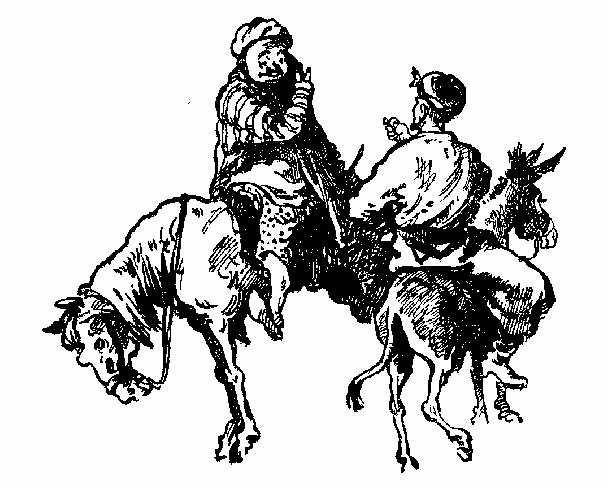
\includegraphics[width=\textwidth]{2.png}
\end{figure}

—~Как~же так? —~возразил слуга. —~Значит, мои перила будут в~пять раз короче твоих?

—~Но~зато они будут в~самом опасном месте! —~с~живостью добавил Ходжа Насреддин.

—~Нет! Я~не~согласен на~такие коротенькие перила! —~решительно сказал слуга. —~Значит, часть моста будет неогороженной! Я~весь бледнею и~покрываюсь холодным потом при мысли о~страшной опасности, угрожающей моему господину! Я~полагаю, что мы~оба должны прочесть молитвы по~сто пятьдесят слов, чтобы перила были с~обеих сторон одинаковыми. Ну, пусть они будут тоненькие, зато с~двух сторон. А~если ты~не~согласен, то~я~в~этом вижу злой умысел против моего господина~— значит, ты~хочешь, чтобы он~свалился с~моста! И~я~сейчас позову людей, и~ты~прямым ходом отправишься в~подземную тюрьму!

—~Тоненькие перила! —~в~ярости вскричал Ходжа Насреддин, чувствуя как~бы слабое пошевеливание кошелька в~своем поясе. —~По-твоему, достаточно огородить этот мост прутиками! Пойми~же, что перила с~одной стороны должны быть непременно толще и~крепче, дабы купцу было за~что ухватиться, если он~оступится и~будет падать!

—~Сама истина говорит твоими устами! —~радостно воскликнул слуга. —~Пусть они будут толще с~моей стороны, а~я~уж~не~пожалею труда и~прочту молитву в~двести слов!

—~А~в~триста не~хочешь? —~злобно сказал Ходжа Насреддин.

Они долго спорили на~дороге. Редкие прохожие, слышавшие обрывки разговора, почтительно кланялись, принимая Ходжу Насреддина и~рябого слугу за~благочестивых паломников, возвращающихся с~поклонения святым местам.

Когда они расставались, кошелек Ходжи Насреддина был легче наполовину: они договорились, что мост, ведущий в~рай, должен быть огорожен для купца с~двух сторон совершенно одинаковыми по~длине и~прочности перилами.

—~Прощай, путник,~— сказал слуга. —~Сегодня мы~с~тобой совершили благочестивое дело.

—~Прощай, добрый, преданный и~добродетельный слуга, столь пекущийся о~спасении души своего хозяина. Скажу еще, что в~споре ты~не~уступишь, наверное, даже самому Ходже Насреддину.

—~Почему ты~вспомнил о~нем? —~насторожился слуга.

—~Да~так. Пришлось к~слову,~— ответил Ходжа Насреддин, подумав про себя: «Эге!.. Да~это, кажется, не~простая птица!»

—~Может быть, ты~приходишься ему каким-нибудь дальним родственником? —~спросил слуга. —~Или знаешь кого-нибудь из~его родственников?

—~Нет, я~никогда не~встречался с~ним. И~я~никого не~знаю из~его родственников.

—~Скажу тебе на~ухо,~— слуга наклонился в~седле,~— я~прихожусь родственником Ходже Насреддину. Я~его двоюродный брат. Мы~вместе провели детские годы.

Ходжа Насреддин, окончательно укрепившись в~своих подозрениях, ничего не~ответил. Слуга нагнулся к~нему с~другой стороны:

—~Его отец, два брата и~дядя погибли. Ты, наверное, слышал, путник?

Ходжа Насреддин молчал.

—~Какое зверство со~стороны эмира! —~воскликнул слуга лицемерным голосом.

Но~Ходжа Насреддин молчал.

—~Все бухарские визири~— дураки! —~сказал вдруг слуга, трепеща от~нетерпения и~алчности, ибо за~поимку вольнодумцев полагалась от~казны большая награда.

Но~Ходжа Насреддин упорно молчал.

—~И~сам наш пресветлый эмир тоже дурак! —~сказал слуга. —~И~еще неизвестно, есть~ли на~небе аллах или его вовсе не~существует.

Но~Ходжа Насреддин молчал, хотя ядовитый ответ давно висел на~самом кончике его языка. Слуга, обманувшийся в~своих надеждах, с~проклятием ударил лошадь нагайкой и~в~два прыжка исчез за~поворотом. Все затихло. Только пыль, взметенная копытами, вилась и~золотилась в~неподвижном воздухе, пронизанная косыми лучами.

«Ну~вот, нашелся все-таки родственничек,~— насмешливо думал Ходжа Насреддин. —~Старик не~солгал мне: шпионов действительно развелось в~Бухаре больше, чем мух, и~надо быть осторожнее, ибо старинная поговорка гласит, что провинившийся язык отрубают вместе с~головой».

Так ехал он~долго, то~омрачаясь при мысли о~своем опустевшем наполовину кошельке, то~улыбаясь при воспоминании о~драке сборщика пошлин с~надменным богачом.


\chapter{}

Достигнув противоположной части города, он~остановился, поручил своего ишака заботам чайханщика, а~сам, не~теряя времени, отправился в~харчевню.

Там было тесно, дымно и~чадно, стоял шум и~гам, жарко пылали печи, и~пламя их~озаряло потных, оголенных до~пояса поваров. Они спешили, кричали, толкая друг друга и~раздавая подзатыльники поварятам, которые с~безумными глазами метались по~всей харчевне, увеличивая давку, галдеж и~сутолоку. Булькали огромные котлы, накрытые деревянными пляшущими кругами, сытный пар сгущался под потолком, где с~гудением вились рои бесчисленных мух. В~сизом чаду яростно шипело, брызгалось масло, светились стенки накаленных жаровен, и~жир, капая с~вертелов на~угли, горел синим душным огнем. Здесь готовили плов, жарили шашлык, варили требуху, пекли пирожки, начиненные луком, перцем, мясом и~курдючным салом, которое, растопившись в~печи, проступало насквозь через тесто и~кипело мелкими пузырьками. Ходжа Насреддин с~большим трудом отыскал место и~втиснулся так плотно, что люди, которых сдавил он~своей спиной и~боками, крякнули. Но~никто не~обиделся и~не~сказал Ходже Насреддину ни~слова, а~сам он~и~подавно не~обижался. Он~всегда любил жаркую давку базарных харчевен, весь этот нестройный гомон, шутки, смех, крики, толкотню, дружное сопение, жевание и~чавканье сотен людей, которым, после целого дня тяжелой работы, некогда разбираться в~кушаньях: несокрушимые челюсти все перемелют~— и~жилы, и~хрящи, а~луженое брюхо все примет, только подавай, чтобы много было и~дешево! Ходжа Насреддин тоже умел закусить основательно: он~съел без передышки три миски лапши, три миски плова и~еще напоследок два десятка пирожков, которые доедал через силу, верный своему правилу никогда ничего не~оставлять в~миске, раз деньги все равно заплачены.

Потом он~полез к~выходу, и~когда, работая изо всех сил локтями, выбрался наконец на~воздух, то~был весь мокрый. Члены его ослабли и~растомились, как будто он~только что побывал в~бане, в~руках у~дюжего мойщика. Вялым шагом, отяжелев от~еды и~жары, наскоро добрался он~до~чайханы, а~добравшись~— заказал себе чаю и~блаженно растянулся на~кошмах. Веки его смыкались, в~голове плыли тихие приятные мысли: «У~меня сейчас много денег; хорошо~бы пустить их~в~оборот и~открыть какую-нибудь мастерскую~— горшечную или седельную; я~ведь знаю эти ремесла. Хватит мне, в~самом деле, скитаться. Разве я~хуже и~глупее других, разве у~меня не~может быть доброй, красивой жены, разве не~может быть у~меня сына, которого носил~бы я~на~руках? Клянусь бородой пророка, из~этого горластого мальчишки выйдет отъявленный плут, я~уж~постараюсь передать ему свою мудрость! Да, решено: Ходжа Насреддин меняет свою беспокойную жизнь. Для начала я~должен купить горшечную или седельную мастерскую...»

Он~занялся подсчетами. Хорошая мастерская стоила самое меньшее триста таньга, у~него~же было сто пятьдесят. С~проклятиями он~вспоминал рябого слугу:

«Да~поразит аллах слепотой этого разбойника, он~отнял у~меня как раз ту~половину, которой недостает сейчас для начала!»

И~удача опять поспешила на~помощь ему. «Двадцать таньга!»~— вдруг сказал кто-то, и~вслед за~этими словами Ходжа Насреддин услышал стук костей, брошенных на~медный поднос.

На~краю помоста, у~самой коновязи, где был привязан ишак, сидели плотным кольцом люди, а~чайханщик стоял над ними, заглядывая сверху через головы.

«Игра! —~догадался Ходжа Насреддин, приподнимаясь на~локте. —~Надо посмотреть хоть издали. Сам~я, конечно, играть не~буду: я~не~такой дурак! Но~почему не~посмотреть умному человеку на~дураков?»

Он~встал и~подошел к~играющим.

—~Глупые люди! —~шепотом сказал он~чайханщику. —~Они рискуют последним в~надежде приобрести большее. И~разве Магомет не~запретил мусульманам денежных игр? Слава богу, я~избавлен от~этой пагубной страсти... Как везет, однако, этому рыжему игроку: он~выигрывает четвертый раз подряд... Смотри, смотри~— он~в~пятый раз выиграл! О~безумец! Он~обольщен ложным призраком богатства, между тем нищета уже вырыла яму на~его пути. Что?.. Он~в~шестой раз выиграл!.. Я~никогда еще не~видел, чтобы человеку так везло. Смотри, он~ставит опять! Поистине, нет предела человеческому легкомыслию; не~может~же он~подряд выигрывать! Вот так и~гибнут люди, поверив в~ложное счастье! Следовало~бы проучить этого рыжего. Ну, пусть он~только выиграет в~седьмой раз, тогда я~сам поставлю против него, хотя в~душе я~враг всяких денежных игр и~давно~бы запретил их~на~месте эмира!..

Рыжий игрок бросил кости и~в~седьмой раз выиграл.

Ходжа Насреддин решительно шагнул вперед, раздвинул игроков и~сел в~кольцо.

—~Я~хочу сыграть с~тобой,~— сказал он~счастливцу, взял кости и~быстро, опытным глазом, проверил их~со~всех сторон.

—~Сколько? —~спросил рыжий глухим голосом. Его била мелкая дрожь~— он~торопился, желая взять как можно больше от~своего мимолетного счастья.

Ходжа Насреддин в~ответ вынул кошелек, отложил на~всякий случай в~карман двадцать пять таньга, остальное высыпал. Серебро зазвенело и~запело на~медном подносе. Игроки встретили ставку легким взволнованным гулом: начиналась большая игра.

Рыжий взял кости и~долго тряс, не~решаясь метнуть. Все затаили дыхание, даже ишак вытянул морду и~насторожил уши. Слышался только стук костей в~кулаке рыжего игрока~— больше ничего. И~от~этого сухого стука вступала в~живот и~в~ноги Ходжи Насреддина истомная слабость. А~рыжий все тряс, придерживая рукав халата, и~не~мог решиться.

Наконец он~метнул. Игроки подались вперед и~сейчас~же откинулись, вздохнув все разом, единой грудью. Рыжий побледнел и~застонал сквозь сжатые зубы.

На~костях было всего три очка~— верный проигрыш, ибо двойка выбрасывается так~же редко, как и~двенадцать, а~все остальное годилось Ходже Насреддину.

Встряхивая в~кулаке кости, он~мысленно благодарил судьбу, столь благосклонную к~нему в~этот день. Но~он~позабыл, что судьба своенравна и~непостоянна и~может с~легкостью изменить, если ей~слишком надоедают. Она решила проучить самоуверенного Ходжу Насреддина и~своим орудием избрала ишака, вернее, его хвост, украшенный на~конце колючками и~репьями. Повернувшись задом к~играющим, ишак взмахнул хвостом, задел по~руке своего хозяина, кости выскочили, и~в~тот~же миг рыжий игрок с~коротким, придушенным воплем упал на~поднос, накрыв собою деньги.

Ходжа Насреддин выбросил два очка.

Долго сидел~он, окаменев, беззвучно шевеля губами,~— все качалось и~плыло перед его остановившимся взором, и~странный звон стоял в~его ушах.

Вдруг он~вскочил, схватил палку и~начал дубасить ишака, бегая за~ним вокруг коновязи.

—~Проклятый ишак, о~сын греха, о~вонючая тварь и~позор всего живущего на~земле! —~кричал Ходжа Насреддин. —~Мало того, что ты~играешь в~кости на~деньги своего хозяина, но~ты~еще и~проигрываешь! Да~облезет твоя подлая шкура, да~пошлет тебе всемогущий аллах яму на~пути, чтобы ты~поломал свои ноги; когда~же ты~наконец издохнешь и~я~избавлюсь от~созерцания твоей гнусной морды?!

Ишак ревел, игроки хохотали, и~громче всех~— рыжий, окончательно поверивший в~свое счастье.

—~Сыграем еще,~— сказал~он, когда Ходжа Насреддин, утомившись и~запыхавшись, отбросил палку. —~Сыграем еще: у~тебя осталось двадцать пять таньга.

При этом он~выставил вперед левую ногу и~слегка пошевелил ею~в~знак пренебрежения к~Ходже Насреддину.

—~Что~ж, сыграем! —~ответил Ходжа Насреддин, решив, что теперь уж~все равно: там, где потеряны сто двадцать таньга, нет смысла жалеть последние двадцать пять.

Он~метнул небрежно, не~глядя,~— и~выиграл.

—~На~все! —~предложил рыжий, бросив на~поднос свой проигрыш.

И~Ходжа Насреддин выиграл опять.

Но~рыжий не~хотел поверить, что счастье повернулось спиной к~нему:

—~На~все!

Так сказал он~семь раз подряд, и~все семь раз проиграл. Поднос был полон денег. Игроки замерли,~— только блеск в~глазах свидетельствовал о~внутреннем огне, пожиравшем~их.

—~Ты~не~можешь выигрывать подряд, если сам шайтан не~помогает тебе! —~вскричал рыжий. —~Ты~должен когда-нибудь проиграть! Здесь на~подносе твоих денег тысяча шестьсот таньга! Согласен~ли ты~метнуть еще раз на~все? Вот деньги, которые я~приготовил, чтобы купить завтра на~базаре товар для моей лавки,~— я~ставлю эти деньги против тебя!

Он~достал маленький запасной кошелек, набитый золотом.

—~Клади на~поднос свое золото! —~вскричал разгорячившийся Ходжа Насреддин.

Никогда еще в~этой чайхане не~было такой большой игры. Чайханщик забыл о~своих давно вскипевших кумганах, игроки дышали тяжело и~прерывисто. Первым бросил кости рыжий и~сразу зажмурился,~— он~боялся взглянуть.

—~Одиннадцать! —~закричали все хором. Ходжа Насреддин понял, что погиб: спасти его могли только двенадцать.

—~Одиннадцать! Одиннадцать! —~твердил в~неистовой радости рыжий игрок. —~Ты~видишь~— у~меня одиннадцать! Ты~проиграл! Ты~проиграл!

Ходжа Насреддин, холодея, взял кости и~уже приготовился их~метнуть, но~вдруг остановился.

—~Повернись-ка задом! —~сказал он~ишаку. —~Ты~сумел проиграть на~трех очках, сумей~же теперь выиграть на~одиннадцати, иначе я~немедля отведу тебя на~живодерню!

Он~взял в~левую руку хвост ишака и~ударил себя этим хвостом по~правой руке, в~которой были зажаты кости.

Всеобщий вопль потряс чайхану, а~сам чайханщик схватился за~сердце и~в~изнеможении опустился на~пол.

На~костях было двенадцать очков.

Глаза рыжего выкатились из~орбит, остекленели на~бледном лице. Он~медленно встал~и, восклицая:

«О, горе мне, горе!»~— вышел, пошатываясь, из~чайханы.

И~говорят, что с~тех пор его не~видели больше в~городе: он~убежал в~пустыню и~там, страшный, заросший весь диким волосом, бродил в~песках и~колючем кустарнике, беспрестанно восклицая: «О, горе мне, горе!»~— пока наконец не~был съеден шакалами. И~никто не~пожалел о~нем, потому что он~был человек жестокий и~несправедливый и~причинил много зла, обыгрывая доверчивых простаков.

А~Ходжа Насреддин, уложив в~переметные сумки выигранное богатство, обнял ишака, крепко поцеловал в~теплый нос и~угостил вкусными, свежими лепешками, чему ишак немало удивился, потому что всего за~пять минут перед этим получил от~своего хозяина совсем другое.


\chapter{}

Памятуя мудрое правило, что лучше держаться подальше от~людей, знающих, где лежат твои деньги, Ходжа Насреддин не~стал задерживаться в~чайхане и~поехал на~базарную площадь. Время от~времени он~оглядывался~— не~следят~ли за~ним, ибо на~лицах игроков да~и~самого чайханщика не~лежала печать добродетели.

Ехать ему было радостно. Теперь он~сможет купить любую мастерскую, две мастерские, три мастерские. Так и~решил он~сделать. «Я~куплю четыре мастерские: гончарную, седельную, портновскую и~сапожную и~посажу в~каждую по~два мастера, а~сам буду только получать деньги. Через два года я~разбогатею, куплю дом с~фонтанами в~саду, повешу везде золотые клетки с~певчими птицами, у~меня будет две или даже три жены и~по~три сына от~каждой...»

Он~с~головой погрузился в~сладостную реку мечтаний. Между тем ишак, не~чувствуя поводьев, воспользовался задумчивостью хозяина~и, встретив на~пути мостик, не~пошел по~нему, подобно всем другим ишакам, а~свернул в~сторону~и, разбежавшись, прыгнул прямо через канаву. «И~когда мои дети вырастут, я~соберу их~и~скажу... —~думал в~это время Ходжа Насреддин. —~Но~почему я~лечу по~воздуху? Неужели аллах решил превратить меня в~ангела и~приделал мне крылья?»

В~ту~же секунду искры, посыпавшиеся из~глаз, убедили Ходжу Насреддина, что крыльев у~него нет. Вылетев из~седла, он~шлепнулся на~дорогу, сажени на~две впереди ишака.

Когда он~с~кряхтеньем и~охами встал, весь перепачканный пылью, ишак, ласково пошевеливая ушами и~сохраняя на~морде самое невинное выражение, подошел к~нему, как~бы приглашая снова занять место в~седле.

—~О~ты, посланный мне в~наказание за~моих грехи и~за~грехи моего отца, деда и~прадеда, ибо, клянусь правотой ислама, несправедливо было~бы столь тяжко наказывать человека за~одни только собственные его грехи! —~начал Ходжа Насреддин дрожащим от~негодования голосом. —~О~ты, презренная помесь паука и~гиены! О~ты, который...

Но~тут он~осекся, заметив каких-то людей, сидевших неподалеку в~тени полуразрушенного забора.

Проклятья замерли на~губах Ходжи Насреддина.

Он~понимал, что человек, попавший на~виду у~других в~смешное и~непочтенное положение, должен сам смеяться громче всех над собой.

Ходжа Насреддин подмигнул сидящим и~широко улыбнулся, показав сразу все свои зубы.

—~Эге! —~сказал он~громко и~весело. —~Вот это я~славно полетел! Скажите, сколько раз я~перевернулся, а~то~я~сам не~успел сосчитать. Ах~ты, шалунишка! —~продолжал~он, добродушно похлопывая ишака ладонью, в~то~время как руки чесались хорошенько отдуть его плетью,~— ах~ты, шалунишка! Он~у~меня такой: чуть зазеваешься, и~он~обязательно уж~что-нибудь сотворит!

Ходжа Насреддин залился веселым смехом, но~с~удивлением заметил, что никто не~вторит ему. Все продолжали сидеть с~опущенными головами и~омраченными лицами, а~женщины, державшие на~руках младенцев, тихо плакали.

«Здесь что-то не~так»,~— сказал себе Ходжа Насреддин и~подошел ближе.

\begin{figure}[h]
\centering
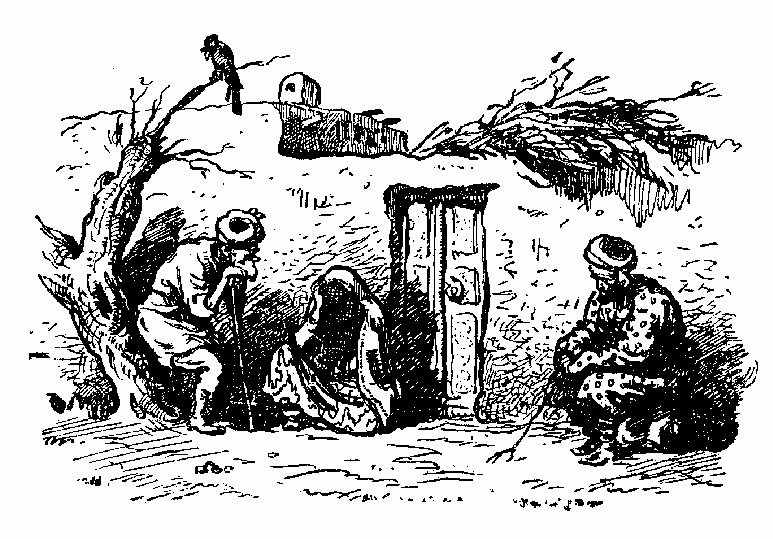
\includegraphics[width=\textwidth]{3.png}
\end{figure}

—~Послушай, почтенный старец,~— обратился он~к~седобородому старику с~изможденным лицом,~— поведай мне, что случилось? Почему я~не~вижу улыбок, не~слышу смеха, почему плачут женщины? Зачем вы~сидите здесь на~дороге в~пыли и~жаре, разве не~лучше сидеть дома в~прохладе?

—~Дома хорошо сидеть тому, у~кого есть дом,~— скорбно ответил старик. —~Ах, прохожий, не~спрашивай~— горе велико, а~помочь ты~все равно не~сможешь. Вот~я, старый, дряхлый, молю сейчас бога, чтобы он~поскорее послал мне смерть.

—~К~чему такие слова! —~укоризненно сказал Ходжа Насреддин. —~Человек никогда не~должен думать об~этом. Поведай мне свое горе и~не~смотри, что я~беден с~виду. Может быть, я~сумею помочь тебе.

—~Мой рассказ будет кратким. Всего час назад по~нашей улице прошел ростовщик Джафар в~сопровождении двух эмирских стражников. А~я~должник ростовщика Джафара, и~завтра утром истекает срок моего долга. И~вот я~изгнан из~своего дома, в~котором прожил всю жизнь, и~нет больше у~меня семьи и~нет угла, где~бы мог я~преклонить голову... А~все имущество мое: дом, сад, скот и~виноградники~— будет продано завтра Джафаром.

Слезы показались на~глазах старика, голос дрожал.

\begin{figure}[h]
\centering
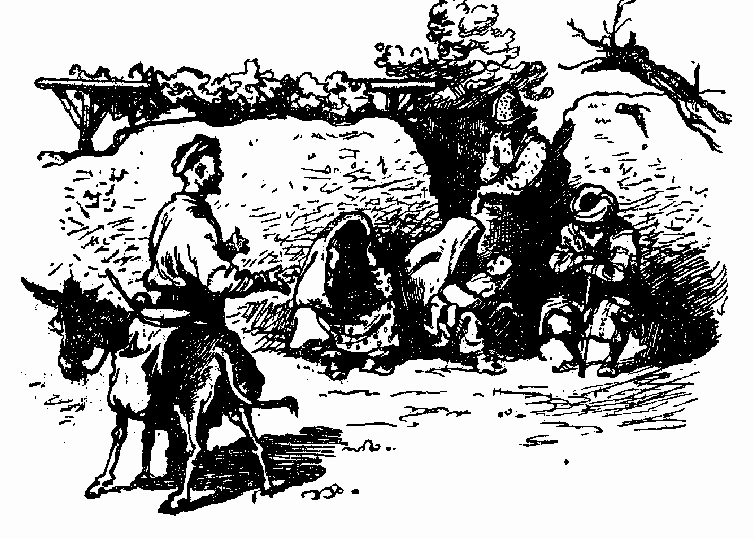
\includegraphics[width=\textwidth]{4.png}
\end{figure}

—~И~много ты~ему должен? —~спросил Ходжа Насреддин.

—~Очень много, прохожий. Я~должен ему двести пятьдесят таньга.

—~Двести пятьдесят таньга! —~воскликнул Ходжа Насреддин. —~И~человек желает себе смерти из-за каких-то двухсот пятидесяти таньга! Ну, ну, стой смирно,~— добавил~он, обращаясь к~ишаку и~развязывая переметную сумку. —~Вот тебе, почтенный старец, двести пятьдесят таньга, отдай их~этому ростовщику, выгони его пинками из~своего дома и~доживай свои дни в~покое и~благоденствии.

Услышав звон серебра, все встрепенулись, а~старик не~мог вымолвить слова и~только глазами, в~которых сверкали слезы, благодарил Ходжу Насреддина.

—~Вот видишь, а~ты~еще не~хотел рассказывать о~своем горе,~— сказал Ходжа Насреддин, отсчитывая последнюю монету и~думая про себя: «Ничего, вместо восьми мастеров я~найму только семь, с~меня и~этого хватит!»

Вдруг женщина, сидевшая рядом со~стариком, бросилась в~ноги Ходже Насреддину и~протянула к~нему с~громким плачем своего ребенка.

—~Посмотри! —~сказала она сквозь рыдания. —~Он~болен, губы его пересохли и~лицо пылает. И~он~умрет теперь, мой бедный мальчик, где-нибудь на~дороге, ибо меня выгнали из~моего дома.

Ходжа Насреддин взглянул на~исхудавшее, бледное личико ребенка, на~его прозрачные руки, потом обвел взглядом лица сидящих. И~когда он~вгляделся в~эти лица, иссеченные морщинами, измятые страданием, и~увидел глаза, потускневшие от~бесконечных слез,~— словно горячий нож вонзился в~его сердце, мгновенная судорога перехватила горло, кровь жаркой волной бросилась в~лицо. Он~отвернулся.

—~Я~вдова,~— продолжала женщина. —~Мой муж, умерший полгода назад, был должен ростовщику двести таньга, и~по~закону долг перешел на~меня.

—~Мальчик в~самом деле болен,~— сказал Ходжа Насреддин. —~И~вовсе не~следует держать его на~солнцепеке, ибо солнечные лучи сгущают кровь в~жилах, как говорит об~этом Авиценна, что, конечно, не~полезно мальчику. Вот тебе двести таньга, возвращайся скорее домой, положи ему примочку на~лоб; вот тебе еще пятьдесят таньга, чтобы ты~могла позвать лекаря и~купить лекарства.

Про себя подумал: «Можно отлично обойтись и~шестью мастерами».

Но~в~ноги ему рухнул огромного роста бородатый каменщик, семью которого завтра должны были продать в~рабство за~долг ростовщику Джафару в~четыреста таньга... «Пять мастеров, конечно, маловато»,~— подумал Ходжа Насреддин, развязывая свою сумку. Не~успел он~ее~завязать, как еще две женщины упали на~колени перед ним, и~рассказы их~были столь жалобны, что Ходжа Насреддин, не~колеблясь, наделил их~деньгами, достаточными для расплаты с~ростовщиком. Увидев, что оставшихся денег едва-едва хватит на~содержание трех мастеров, он~решил, что в~таком случае не~стоит и~связываться с~мастерскими, и~щедрой рукой принялся раздавать деньги остальным должникам ростовщика Джафара.

В~сумке осталось не~больше пятисот таньга. И~тогда Ходжа Насреддин заметил в~стороне еще одного человека, который не~обратился за~помощью, хотя на~лице его было ясно написано горе.

—~Эй~ты, послушай! —~позвал Ходжа Насреддин. —~Зачем ты~сидишь здесь? Ведь за~тобой нет долга ростовщику?

—~Я~должен ему,~— глухо сказал человек. —~Завтра я~сам пойду в~цепях на~невольничий рынок.

—~Почему~же ты~молчал до~сих пор?

—~О~щедрый, благодетельный путник, я~не~знаю, кто~ты. Святой~ли Богаэддин, вышедший из~своей гробницы, чтобы помочь беднякам, или сам Гарун-аль-Рашид? Я~не~обратился к~тебе только потому, что и~без меня ты~уже очень сильно потратился, а~я~должен больше всех~— пятьсот таньга, и~я~боялся, что если ты~дашь мне, то~не~хватит старикам и~женщинам.

—~Ты~справедлив, благороден и~совестлив,~— сказал растроганный Ходжа Насреддин. —~Но~я~тоже справедлив, благороден и~совестлив, и, клянусь, ты~не~пойдешь завтра в~цепях на~невольничий рынок. Держи полу!

Он~высыпал из~переметной сумки все деньги до~последней таньга. Тогда человек, придерживая левой рукой полу халата, обнял правой рукой Ходжу Насреддина и~припал в~слезах к~его груди.

Ходжа Насреддин обвел взглядом всех спасенных людей, увидел улыбки, румянец на~лицах, блеск в~глазах.

—~А~ты~в~самом деле здорово полетел со~своего ишака, -сказал вдруг огромный бородатый каменщик, захохотав, и~все разом захохотали~— мужчины грубыми голосами, а~женщины~— тонкими, и~заулыбались дети, протягивая ручонки к~Ходже Насреддину, а~сам он~смеялся громче всех.

—~О! —~говорил~он, корчась от~смеха,~— вы~еще не~знаете, какой это ишак! Это такой проклятый ишак!..

—~Нет! —~перебила женщина с~больным ребенком на~руках. —~Не~говори так про своего ишака. Это самый умный, самый благородный, самый драгоценный в~мире ишак, равных ему никогда еще не~было и~не~будет. Я~согласна всю жизнь ухаживать за~ним, кормить его отборным зерном, никогда не~утруждать работой, чистить скребницей, расчесывать хвост ему гребнем. Ведь если~бы этот несравненный и~подобный цветущей розе ишак, наполненный одними лишь добродетелями, не~прыгнул через канаву и~не~выбросил тебя из~седла, о~путник, явившийся перед нами, как солнце во~мгле,~— ты~проехал~бы мимо, не~заметив нас, а~мы~не~посмели~бы остановить тебя!

—~Она права,~— глубокомысленно заметил старик. —~Мы~во~многом обязаны своим спасением этому ишаку, который поистине украшает собою мир и~выделяется, как алмаз, среди всех других ишаков.

Все начали громко восхвалять ишака и~наперебой совали ему лепешки, жареную кукурузу, сушеные абрикосы и~персики. Ишак, отмахиваясь хвостом от~назойливых мух, невозмутимо и~важно принимал подношения, однако заморгал все-таки глазами при виде плетки, которую исподтишка показывал ему Ходжа Насреддин.

Но~время шло своим чередом, удлинились тени, краснолапые аисты, крича и~хлопая крыльями, опускались в~гнезда, откуда навстречу им~тянулись жадно раскрытые клювы птенцов.

Ходжа Насреддин начал прощаться.

Все кланялись и~благодарили его:

—~Спасибо тебе. Ты~понял наше горе.

—~Еще~бы мне не~понять,~— ответил~он,~— если я~сам не~далее как сегодня потерял четыре мастерских, где у~меня работали восемь искуснейших мастеров, дом и~сад, в~котором били фонтаны и~висели на~деревьях золотые клетки с~певчими птицами. Еще~бы мне не~понять!

Старик прошамкал своим беззубым ртом:

—~Мне нечем отблагодарить тебя, путник. Вот единственное, что захватил~я, покидая дом. Это~— коран, священная книга; возьми~ее, и~да~будет она тебе путеводным огнем в~житейском море.

Ходжа Насреддин относился к~священным книгам без всякого почтения, но, не~желая обидеть старика, взял коран, уложил в~переметную сумку и~вскочил в~седло.

—~Имя, имя! —~закричали все хором. —~Скажи нам свое имя, чтобы мы~знали, кого благодарить в~молитвах.

—~Зачем вам знать мое имя? Истинная добродетель не~нуждается в~славе, что~же касается молитв, то~у~аллаха есть много ангелов, извещающих его о~благочестивых поступках... Если~же ангелы ленивы и~нерадивы и~спят где-нибудь на~мягких облаках, вместо того чтобы вести счет всем благочестивым и~всем богохульным делам на~земле, то~молитвы ваши все равно не~помогут, ибо аллах был~бы просто глуп, если~бы верил людям на~слово, не~требуя подтверждения от~доверенных лиц.

Одна из~женщин вдруг тихо ахнула, за~ней~— вторая, потом старик, встрепенувшись, уставился во~все глаза на~Ходжу Насреддина. Но~Ходжа Насреддин торопился и~ничего не~заметил.

—~Прощайте. Да~пребудут мир и~благоденствие над вами.

Сопровождаемый благословениями, он~скрылся за~поворотом дороги.

Оставшиеся молчали, в~глазах у~всех светилась одна мысль.

Молчание нарушил старик. Он~сказал проникновенно и~торжественно:

—~Только один человек во~всем мире может совершить такой поступок, и~только один человек в~мире умеет так разговаривать, и~только один человек в~мире носит в~себе такую душу, свет и~тепло которой обогревают всех несчастных и~обездоленных, и~этот человек~— он, наш...

—~Молчи! —~быстро перебил второй. —~Или ты~забыл, что заборы имеют глаза, камни имеют уши, и~многие сотни собак кинулись~бы по~его следу.

—~Ты~прав,~— добавил третий. —~Мы~должны молчать, ибо он~ходит сейчас по~канату, и~достаточно малейшего толчка, чтобы погубить его.

—~Пусть мне лучше вырвут язык, чем я~произнесу где-нибудь вслух его имя! —~сказала женщина с~больным ребенком на~руках.

—~Я~буду молчать,~— воскликнула вторая женщина,~— ибо я~согласна скорее умереть сама, чем подарить ему нечаянно веревку!

Так сказали все, кроме бородатого и~могучего каменщика, который не~отличался остротой ума~и, прислушиваясь к~разговорам, никак не~мог понять, почему собаки должны бегать по~следам этого путника, если он~не~мясник и~не~продавец вареной требухи; если~же этот путник канатоходец, то~почему имя его так запретно для произнесения вслух, и~почему женщина согласна скорее умереть, чем подарить своему спасителю веревку, столь необходимую в~его ремесле? Здесь каменщик совсем уж~запутался, сильно засопел, шумно вздохнул и~решил больше не~думать, опасаясь сойти с~ума.

Ходжа Насреддин уехал тем временем далеко, а~перед его глазами все стояли изможденные лица бедняков; он~вспоминал больного ребенка, лихорадочный румянец на~его щеках и~запекшиеся в~жару губы; вспоминал седины старика, выброшенного из~родного дома,~— и~ярость поднималась из~глубины его сердца.

Он~не~мог усидеть в~седле, спрыгнул и~пошел рядом с~ишаком, отшвыривая пинками попадавшиеся под ноги камни.

—~Ну, подожди, ростовщик, подожди! —~шептал~он, и~зловещий огонь разгорался в~его черных глазах. —~Мы~встретимся, и~твоя участь будет горька! И~ты, эмир,~— продолжал~он,~— трепещи и~бледней, эмир, ибо~я. Ходжа Насреддин, в~Бухаре! О~презренные пиявки, сосущие кровь из~моего несчастного народа, о~жадные гиены и~вонючие шакалы, не~вечно вам блаженствовать и~не~вечно народу мучиться! Что~же касается тебя, ростовщик Джафар, то~пусть на~веки веков покроется мое имя позором, если я~не~расквитаюсь с~тобой за~все горе, которое причиняешь ты~беднякам!


\chapter{}

Даже для Ходжи Насреддина, повидавшего в~жизни многое, этот день~— первый день пребывания на~родине~— был слишком беспокоен и~богат приключениями. Ходжа Насреддин устал и~стремился укрыться куда-нибудь в~тихое место на~отдых.

—~Нет! —~вздохнул~он, увидев издали множество людей, столпившихся вокруг водоема. —~Видно, мне сегодня не~суждено отдохнуть! Вон опять что-то случилось!

Водоем лежал в~стороне от~большой дороги, и~Ходжа Насреддин мог~бы проехать мимо, но~не~таков был наш Ходжа Насреддин, чтобы упустить случай вмешаться в~спор, скандал или драку.

Ишак, в~совершенстве изучивший за~долгие годы характер своего господина, повернул, не~дожидаясь приказаний, к~водоему.

—~Что случилось? Кого убили? Кого обокрали? —~закричал Ходжа Насреддин, направив ишака в~самую гущу народа. —~А~ну-ка расступитесь! Дорогу! Дорогу!

Когда он~пробрался сквозь толпу и~подъехал к~самому краю большого, покрытого зеленоватой плесенью водоема, то~увидал необычайное. В~трех шагах от~берега тонул человек. Он~то~выныривал, то~опять погружался, пуская со~дна большие пузыри.

На~берегу суетилось множество людей; они тянулись к~тонущему, стараясь ухватить его за~халат, но~руки их~не~доставали на~каких-нибудь поларшина.

—~Давай руку! Давай! Давай! —~кричали они. Тонущий словно~бы не~слышал. Он~не~подавал им~руки, продолжая равномерно погружаться и~снова выныривать. В~соответствии с~его странствиями на~дно и~обратно по~водоему расходились ленивые волны и~с~тихим плеском лизали берег.

—~Странно! —~сказал Ходжа Насреддин, наблюдая. —~Очень странно! Какая может быть причина этому? Почему он~не~протягивает руки? Может быть, он~искусный водолаз и~ныряет на~спор, но~почему тогда он~в~халате?

Ходжа Насреддин задумался. Пока он~думал, тонущий успел вынырнуть раза четыре, причем с~каждым разом пребывал на~дне все дольше и~дольше.

—~Очень странно! —~повторил Ходжа Насреддин, спешиваясь. —~Обожди здесь,~— обратился он~к~ишаку,~— а~я~подойду взглянуть поближе.

Тонущий в~это время погрузился глубоко и~не~показывался так долго, что некоторые на~берегу начали уже творить заупокойные молитвы. Но~вдруг он~показался опять.

—~Давай руку! Давай! Давай! —~закричали люди, протягивая к~нему руки, но~он, посмотрев белыми глазами и~не~протянув руки, опять пошел безмолвно и~плавно ко~дну.

—~Ах~вы, недогадливые чудаки! —~сказал Ходжа Насреддин. —~Разве не~видите вы~по~дорогому халату и~по~шелковой чалме, что этот человек~— мулла или богатый вельможа? И~неужели вы~до~сих пор не~изучили характера мулл и~вельмож и~не~знаете, каким способом надо вытаскивать их~из~воды?

—~Вытаскивай скорее, если ты~знаешь! —~закричали в~толпе. —~Спасай его, он~показался. Вытаскивай!

—~Подождите,~— ответил Ходжа Насреддин. —~Я~не~закончил еще своей речи. Где, спрашиваю я~вас, встречали вы~муллу или вельможу, который когда-нибудь что-нибудь кому-нибудь давал? Запомните, о~невежды: муллы и~вельможи никогда ничего не~дают, они только берут. И~спасать их~из~воды надо соответственно их~характеру. Вот, смотрите!

—~Но~ты~уже опоздал,~— кричали из~толпы. —~Он~уке не~вынырнет больше.

—~Вы~думаете, что водяные духи так легко примут к~себе муллу или вельможу? Вы~ошибаетесь. Водяные духи постараются всеми силами избавиться от~него.

Ходжа Насреддин присел на~корточки и~стал терпеливо ждать, наблюдая за~пузырями, что восходили со~дна и~плыли к~берегу, подгоняемые легким ветром.

Наконец что-то темное стало подниматься из~глубины. Тонущий показался на~поверхности~— в~последний раз, если~бы не~Ходжа Насреддин.

—~На! —~крикнул Ходжа Насреддин, сунув ему руку,~— На!

Тонущий судорожно вцепился в~протянутую руку. Ходжа Насреддин поморщился от~боли.

И~потом на~берегу долго не~могли разжать пальцев спасенного.

Несколько минут лежал он~без движения, окутанный водорослями и~облепленный зловонной тиной, скрывавшей черты его лица. Потом изо рта, из~носа, из~ушей у~него хлынула вода.

—~Сумка! Где моя сумка? —~простонал он~и~не~успокоился до~тех пор, пока не~нащупал на~боку сумку. Тогда он~стряхнул с~себя водоросли и~полой халата вытер тину с~лица. И~Ходжа Насреддин отшатнулся: настолько безобразно было это лицо с~плоским перешибленным носом и~вывернутыми ноздрями, с~бельмом на~правом глазу. Вдобавок он~был еще и~горбат.

—~Кто мой спаситель? —~спросил он~скрипучим голосом, обводя столпившихся людей своим единственным оком.

—~Вот он! —~загудели все, выталкивая вперед Ходжу Насреддина.

—~Подойди сюда, я~вознагражу тебя. —~Спасенный запустил руку в~свою сумку, где еще хлюпала вода, и~достал горсть мокрого серебра. —~Впрочем, в~том, что ты~меня вытащил, нет ничего особенного и~удивительного, я, пожалуй, и~сам~бы выплыл,~— продолжал он~сварливым голосом.

\begin{figure}[p]
\centering
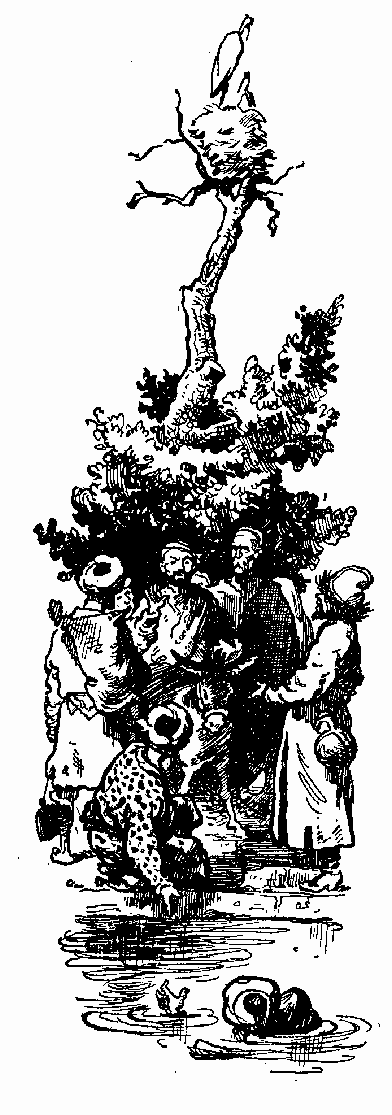
\includegraphics[scale=0.6]{5.png}
\end{figure}

Пока он~говорил, горсть его~— от~слабости~ли, а~может быть, и~по~другой причине~— постепенно разжималась, и~деньги с~тихим звоном текли сквозь пальцы обратно в~сумку. Наконец в~руке осталась одна монета~— полтаньга; он~со~вздохом протянул монету Ходже Насреддину:

—~Вот тебе деньги. Пойди на~базар и~купи миску плова.

—~Здесь не~хватит на~миску плова,~— сказал Ходжа Насреддин.

—~Ничего, ничего. А~ты~возьми плов без мяса.

—~Теперь вам понятно,~— обратился Ходжа Насреддин к~остальным,~— что я~спасал его действительно в~полном соответствии с~его характером.

Он~направился к~своему ишаку.

На~пути остановил его человек~— высокий, тощий, жилистый, угрюмого и~неприветливого вида, с~руками, черными от~угля и~копоти, с~кузнечными клещами за~поясом.

—~Что тебе, кузнец? —~спросил Ходжа Насреддин.

—~Знаешь~ли ты,~— ответил кузнец, смерив Ходжу Насреддина с~ног до~головы недобрым взглядом,~— знаешь~ли ты, кого спас в~самую последнюю минуту, после которой его никто~бы уже не~спас? И~знаешь~ли ты, сколько слез прольется теперь из-за твоего поступка и~сколько людей потеряют свои дома, поля и~виноградники и~пойдут на~невольничий рынок, а~потом~— в~цепях~— по~Большой Хивинской дороге?

Ходжа Насреддин воззрился на~него с~удивлением:

—~Я~не~понимаю тебя, кузнец! Разве достойно человека и~мусульманина пройти мимо тонущего, не~протянув ему руку помощи!

—~Что~же, по-твоему, надо спасать от~гибели всех ядовитых змей, всех гиен и~каждую ехидну! —~воскликнул кузнец и~вдруг, сообразив что-то, добавил: —~Да~здешний~ли ты?

—~Нет! Я~приехал издалека.

—~Значит, ты~не~знаешь, что спасенный тобой человек~— злодей и~кровопийца и~каждый третий человек в~Бухаре стонет и~плачет из-за него!

Страшная догадка мелькнула в~голове Ходжи Насреддина.

—~Кузнец! —~сказал он~дрогнувшим голосом, боясь поверить в~свою догадку. —~Скажи мне имя спасенного мною!

—~Ты~спас ростовщика Джафара, да~будет он~проклят и~в~этой и~в~будущей жизни, и~да~поразят гнойные язвы все его племя до~четырнадцатого колена! —~ответил кузнец.

—~Как! —~вскричал Ходжа Насреддин. —~Что ты~говоришь, кузнец! О~горе мне, о~позор на~мою голову! Неужели я~своими руками вытащил из~воды эту змею! Поистине, нет искупления такому греху! О~горе, о~позор и~несчастье!

Его раскаяние тронуло кузнеца, он~немного смягчился:

—~Успокойся, путник, теперь уж~ничего не~поделаешь. И~надо~же было тебе подъехать как раз в~эту минуту к~водоему. И~почему твой ишак не~заупрямился где-нибудь и~не~задержался в~дороге! За~это время ростовщик как раз успел~бы потонуть.

—~Этот ишак! —~сказал Ходжа Насреддин. —~Если он~и~задерживается в~дороге, то~для того только, чтобы очистить от~денег мои переметные сумки: ему, видишь~ли, тяжело возить их~с~деньгами. А~уж~если мне предстоит опозорить себя спасением ростовщика, то~можешь не~сомневаться: этот ишак доставит на~место как раз вовремя!

—~Да! —~сказал кузнец. —~Но~сделанного не~воротишь. Не~загонять~же теперь ростовщика обратно в~пруд!

Ходжа Насреддин встрепенулся:

—~Я~совершил нехорошее дело, но~я~же исправлю его! Слушай, кузнец! Клянусь, что ростовщик Джафар будет утоплен мною. Клянусь бородой моего отца, что он~будет утоплен мною в~этом~же самом пруду! Запомни мою клятву, кузнец! Я~никогда еще не~говорил на~ветер. Ростовщик будет утоплен! И~когда ты~об~этом услышишь на~базаре, знай, что я~искупил свою вину перед жителями Благородной Бухары!


\chapter{}

На~город уже опускались сумерки, когда Ходжа Насреддин добрался до~базарной площади.

Зажигались яркие костры в~чайханах, и~скоро вся площадь опоясалась огнями. Завтра предстоял большой базар~— и~один за~другим шли мягкой поступью верблюжьи караваны, исчезали в~темноте, а~воздух был все еще полон мерным, медным и~печальным звоном бубенцов; и~когда затихали в~отдалении бубенцы одного каравана, им~на~смену начинали стонать бубенцы другого, вступающего на~площадь, и~это было нескончаемо, словно сама темнота над площадью тихо звенела, дрожала, переполнившись звуками, принесенными сюда со~всех концов мира. Здесь~— невидимые~— стонали бубенцы индийские и~афганские, аравийские, иранские и~египетские; Ходжа Насреддин все слушал и~слушал и~готов был слушать без конца. Рядом в~чайхане ударил, загудел бубен, ему ответили струны дутара. И~невидимый певец высоко под самые звезды поднял звенящий напряженный голос: он~пел о~своей возлюбленной, он~жаловался на~нее.

Под эту песню пошел Ходжа Насреддин искать ночлега.

—~У~нас на~двоих с~ишаком есть полтаньга,~— сказал он~чайханщику.

—~Можешь переночевать на~кошме за~полтаньга,~— ответил чайханщик. —~Одеяла не~получишь.

—~А~где мне привязать ишака?

—~Вот еще, буду я~заботиться о~твоем ишаке.

Коновязи около чайханы не~было. Ходжа Насреддин заметил какую-то железную скобу, торчавшую из-под помоста. К~этой скобе он~и~привязал ишака, не~потрудившись посмотреть, к~чему~же приделана скоба, потом вошел в~чайхану и~улегся: он~очень устал.

Сквозь дрему он~услышал вдруг свое имя. Он~приоткрыл глаза.

Неподалеку сидели, собравшись в~кружок, и~пили чай какие-то люди, приехавшие на~базар,~— погонщик, пастух и~два ремесленника. Один из~них вполголоса говорил:

—~Рассказывают еще так о~Ходже Насреддине: однажды в~Багдаде шел он~по~базару и~вдруг услышал шум и~крик, доносившиеся из~харчевни. Наш Ходжа Насреддин, как вам известно, человек любопытный,~— он~заглянул в~харчевню. И~видит, что толстый, красномордый харчевник трясет за~шиворот какого-то нищего и~требует денег, а~нищий не~хочет платить.

«Что за~шум? —~спрашивает наш Ходжа Насреддин. —~Что вы~не~поделили?»

«Вот этот бродяга,~— закричал в~ответ харчевник,~— этот презренный оборванец и~жулик зашел сейчас в~мою харчевню, да~отсохнут все его внутренности, вынул из-за пазухи лепешку и~долго держал ее~над жаровней, пока лепешка не~пропиталась насквозь запахом шашлыка и~не~стала от~этого вдвое вкуснее. Потом этот нищий сожрал лепешку, а~теперь не~хочет платить, да~выпадут все его зубы и~облезет кожа!»

«Это правда?»~— строго спросил наш Ходжа Насреддин у~нищего, который не~мог от~страха вымолвить слова и~только кивнул в~ответ головой.

«Нехорошо,~— сказал Ходжа Насреддин. —~Очень нехорошо пользоваться бесплатно чужим добром».

«Ты~слышишь, оборванец, что тебе говорит этот почтенный и~достойный человек!»~— обрадовался харчевник.

«У~тебя есть деньги?»~— обратился Ходжа Насреддин к~нищему. Тот молча достал из~кармана последние медяки. Харчевник уже протянул свою жирную лапу за~ними.

«Подожди, о~почтенный! —~остановил его Ходжа Насреддин. —~Давай-ка сначала сюда твое ухо».

И~он~долго звенел зажатыми в~кулаке деньгами над самым ухом харчевника. А~потом, вернув деньги нищему, сказал:

«Иди с~миром, бедный человек!»

«Как! —~закричал харчевник. —~Но~я~не~получил платы!»

«Он~заплатил тебе полностью, и~вы~в~расчете,~— ответил наш Ходжа Насреддин. —~Он~нюхал, как пахнет твой шашлык, а~ты~слышал, как звенят его деньги».

Все в~чайхане так и~покатились со~смеху. Один поспешно предупредил:

—~Тише. А~то~сразу догадаются, что мы~говорим о~Ходже Насреддине.

«Откуда они только знают? —~улыбался про себя Ходжа Насреддин. —~Это, правда, было не~в~Багдаде, а~в~Стамбуле, но~все равно~— откуда они знают?»

Начал вполголоса рассказывать второй~— в~одежде пастуха и~в~цветной чалме, что выдавало в~нем жителя Бадахшана:

—~Рассказывают еще и~так. Однажды Ходжа Насреддин шел мимо огорода муллы. Мулла как раз собирал в~мешок тыквы и~по~жадности нагрузил мешок так, что не~мог даже и~поднять его, не~только нести. Вот стоит и~думает: «Как~же мне доставить мешок домой?» Увидел прохожего и~обрадовался:

«Послушай, сын мой. Не~возьмешься~ли ты~донести до~моего дома этот мешок?»

А~у~Ходжи Насреддина как раз не~было денег.

«А~сколько ты~мне заплатишь?»~— спросил он~муллу.

«О~сын мой! На~что тебе деньги? Пока ты~будешь нести тыквы, я~по~дороге поведаю тебе три премудрости, и~они сделают тебя счастливым на~всю жизнь».

«Интересно, какие премудрости обещает открыть мне мулла?»~— думает про себя наш Ходжа Насреддин.

Его разобрало любопытство. Он~взвалил на~плечи мешок и~понес. А~дорога круто поднималась в~гору и~шла над обрывом. Когда Ходжа Насреддин остановился отдохнуть, мулла сказал с~таинственным и~важным видом:

«Слушай первую премудрость, и~большей не~было в~мире никогда со~времен Адама, и~если ты~постигнешь всю глубину~ее, то~это будет равносильно познанию тайного смысла букв~— Алиф, Лам, Ра, которыми Магомет, пророк и~учитель наш, открывает вторую суру корана. Слушай внимательно: если кто-нибудь тебе скажет, что ходить пешком лучше, чем ездить верхом,~— ты~не~верь этому человеку. Запомни мои слова и~думай над ними неотступно днем и~ночью~— и~тогда ты~постигнешь заключающуюся в~них премудрость. Но~эта премудрость~— ничто в~сравнении со~второй премудростью, которую я~тебе поведаю вон у~того дерева. Видишь~— во-он впереди!»

«Ладно! —~думает про себя Ходжа Насреддин. —~Погоди, мулла!»

Обливаясь потом, он~дотащил мешок до~дерева.

Мулла поднял палец:

"Открой свои уши и~внимай, ибо вторая премудрость включает в~себя весь коран и~половину шариата и~еще одну четверть книги тариката\footnote{Тарикат~— религиозно-философские наставления, которыми руководствовались члены религиозных суфийских братств, искавшие пути самосовершенствования.}. И~постигший эту премудрость никогда не~собьется с~пути добродетели и~никогда не~оступится на~дороге истины. Постарайся~же, о~сын мой, понять эту премудрость и~радуйся, что получил ее~бесплатно. Вторая премудрость гласит: если тебе кто-нибудь скажет, что бедному легче жить, чем богатому, ты~не~верь этому человеку.

Но~даже и~эта вторая премудрость~— ничто рядом с~третьей, сияние которой можно сравнить только с~ослепительным блеском солнца и~глубину которой можно сравнить только с~глубиной океана. Третью премудрость я~поведаю тебе у~ворот моего дома. Идем скорее, ибо я~уже отдохнул".

«Подожди, мулла! —~отвечает наш Ходжа Насреддин. —~Я~наперед знаю твою третью премудрость. Ты~хочешь у~ворот своего дома сказать мне, что умный человек всегда может заставить глупца бесплатно тащить мешок с~тыквами».

Пораженный мулла отшатнулся. Ходжа Насреддин слово в~слово угадал его третью премудрость.

«Но~послушай теперь, мулла, мою одну-единственную премудрость, которая стоит всех твоих,~— продолжал Ходжа Насреддин. —~И~моя премудрость, клянусь Магометом, столь ослепительна и~столь глубока, что включает в~себя весь ислам с~кораном, шариатом, книгой тариката и~всеми другими книгами, и~всю буддийскую веру, и~всю иудейскую веру, и~все христианские заблуждения. Нет, никогда не~было и~не~будет впредь премудрости более достоверной, чем~та, которую я~поведаю тебе сейчас, о~мулла! Но~приготовься, чтобы не~поразила тебя слишком эта премудрость, ибо от~нее легко потерять рассудок~— настолько она поразительна, ослепительна и~необъятна. Подготовь~же свой рассудок, мулла, и~слушай: если кто-нибудь скажет тебе, что эти вот самые тыквы не~разбились~— плюнь в~лицо тому человеку, назови его лжецом и~прогони из~дома!»

С~этими словами Ходжа Насреддин поднял мешок и~бросил вниз с~крутого обрыва.

Тыквы сыпались из~мешка, прыгали и~звучно раскалывались, налетая на~камни.

«О~горе мне! О~великий убыток и~разорение!»~— закричал мулла.

И~начал он~кричать, причитать, царапать лицо, и~всем своим видом вполне походил на~безумного.

«Вот видишь! —~поучительно молвил Ходжа Насреддин. —~Ведь я~предупреждал, что от~моей премудрости рассудок твой может легко помутиться!»

Слушавшие залились веселым смехом.

Ходжа Насреддин, лежа в~углу на~пыльной блохастой кошме, думал:

"Они и~это узнали! Но~откуда? Ведь нас было только двое над обрывом, и~я~никому не~рассказывал.

Вероятно, рассказал сам мулла, догадавшись впоследствии, кто тащил его тыквы".

Начал третий рассказчик:

—~Однажды Ходжа Насреддин возвращался из~города в~турецкую деревню, где тогда жил; почувствовав себя утомленным, он~лег отдохнуть на~берег речки~— и~незаметно уснул, овеваемый благоуханным дыханием весеннего ветерка. И~приснилось ему, что он~умер. «Если я~мертв,~— решил про себя наш Ходжа Насреддин,~— то~я~не~должен шевелиться и~не~должен открывать глаза». Так и~лежал он~долгое время без движения на~мягкой траве и~нашел, что быть мертвым не~так уж~плохо: лежи себе да~лежи безо всяких забот и~хлопот, что неотступно преследуют нас в~нашем земном, бренном существовании.

Мимо шли какие-то путники, увидели Ходжу Насреддина.

«Смотрите! —~сказал один. —~Это мусульманин».

«Он~мертв»,~— добавил второй.

«Надо отнести его в~ближайшую деревню, чтобы его там обмыли и~похоронили достойно»,~— предложил третий, назвав как раз ту~самую деревню, куда на~правлялся Ходжа Насреддин.

Путники срубили несколько молодых деревьев, устроили носилки и~взвалили на~них Ходжу Насреддина.

Они долго несли его, а~он~лежал без движения, не~открывая глаз, как и~подобает мертвецу, душа которого стучится уже в~двери рая.

Вдруг носилки остановились. Путники начали спорить~— где брод. Один звал направо, второй налево, третий предлагал идти через речку напрямик.

Ходжа Насреддин приоткрыл чуть-чуть один глаз и~увидел, что путники стоят перед самым глубоким, быстрым и~опасным местом реки, где уже не~раз тонули неосторожные. «О~себе самом я~не~беспокоюсь,~— подумал Ходжа Насреддин. —~Я~все равно мертв, и~мне безразлично теперь, где лежать~— в~могиле или на~речном дне. Но~этих путников следует предупредить, иначе они из-за своего внимания ко~мне могут лишиться жизни, что было~бы с~моей стороны чистейшей неблагодарностью».

Он~приподнялся на~носилках~и, указывая рукой в~сторону брода, произнес слабым голосом:

«О~путники, когда я~был жив, то~всегда переходил эту речку вон у~тех тополей».

И~он~опять закрыл глаза. Путники, поблагодарив Ходжу Насреддина за~указание, потащили носилки дальше, читая громко молитвы о~спасении его души. Пока слушавшие да~и~сам рассказчик хохотали, подталкивая друг друга локтями. Ходжа Насреддин с~неудовольствием бормотал:

—~Все переврали. Во-первых, мне не~приснилось, что я~умер. Не~такой уж~я~дурак, чтобы не~отличить самого себя живого от~самого себя мертвого. Я~даже хорошо помню, что меня все время кусала блоха и~мне отчаянно хотелось почесаться,~— разве это не~доказывает с~полной очевидностью, что я~был действительно жив, ибо в~противном случае~я, конечно, не~мог~бы чувствовать укусов блохи. Просто я~устал, и~мне не~хотелось идти, а~эти путники были ребята здоровые: что им~стоило сделать небольшой крюк и~отнести меня в~деревню? Но~когда они решили переходить реку там, где глубина была в~три человеческих роста, я~их~остановил, заботясь, впрочем, не~столько о~своей семье, ибо у~меня ее~нет, сколько об~их~семьях. И~сейчас~же я~испробовал горького плода неблагодарности: вместо того чтобы сказать мне спасибо за~своевременное предупреждение, они вытряхнули меня из~носилок, бросились на~меня с~кулаками~— и~наверняка сильно~бы избили меня, если~бы не~резвость моих ног!.. Удивляюсь, до~чего могут люди исказить и~переврать действительно случившееся.

Между тем четвертый начал свой рассказ:

—~И~говорят еще о~Ходже Насреддине такое. Он, Ходжа Насреддин, жил около полугода в~одной деревне и~весьма прославился между жителями находчивостью в~ответах и~остротою своего ума...

Ходжа Насреддин насторожился. Где слышал он~этот голос~— негромкий, но~внятный, с~едва заметной хрипотцой? И~совсем недавно... Может быть, даже сегодня... Но~как ни~старался~— вспомнить не~мог.

Рассказчик продолжал:

—~Губернатор той области направил однажды в~деревню, где жил Ходжа Насреддин, одного из~своих слонов на~постой и~прокормление от~жителей. Слон был неописуемо прожорлив. Он~съедал за~одни сутки пятьдесят мер ячменя, пятьдесят мер джугары, пятьдесят мер кукурузы и~сто снопов свежего клевера. Через две недели жители деревни скормили слону все свои запасы, разорились и~впали в~уныние. И~решили, наконец, послать Ходжу Насреддина к~самому губернатору с~просьбой, чтобы слона убрали из~деревни...

И~вот они пошли к~Ходже Насреддину, стали его просить, он~согласился, оседлал своего ишака, который, как это известно всему миру, своим упрямством, злонравием и~леностью подобен шакалу, пауку, гадюке и~лягушке, слитым воедино,~— и, оседлав его, отправился к~губернатору, причем не~забыл уговориться заранее с~жителями о~плате за~свое дело, и~плату назначил столь большую, что многие были вынуждены продать свои дома и~остались нищими по~милости Ходжи Насреддина.

—~Кгм! —~донеслось из~угла. Это Ходжа Насреддин, ворочавшийся и~подпрыгивавший на~кошме, с~трудом удерживал клокочущую в~груди ярость.

Рассказчик продолжал:

—~И~он. Ходжа Насреддин, пришел во~дворец и~долго стоял в~толпе слуг и~приживалов, ожидая, когда сиятельный губернатор, блистающий великолепием и~мощью, подобно солнцу, соблаговолит обратить к~нему свой пресветлый взор, изливающий на~одних -счастье, а~на~других~— гибель. И~когда губернатор, сверкающий среди окружавших его, как серебристая луна среди звезд или стройный благоуханный кипарис среди низкорослого кустарника, соблаговолил осчастливить Ходжу Насреддина и~обратил к~нему свой лик, на~котором благородство и~мудрость сочетались, как рубин и~алмаз в~одном перстне, когда, говорю~я, губернатор обратил к~нему свой лик, то~от~страха и~удивления перед таким великолепием колени Ходжи Насреддина затряслись, как шакалий хвост, и~кровь стала медленнее ходить в~жилах, он~весь покрылся потом и~сделался бледен как мел.

—~Кгм! —~донеслось из~угла, но~рассказчик не~обратил на~это внимания и~продолжал:

—~«Что ты~хочешь?»~— спросил губернатор благородным и~звучным голосом, напоминающим рыкание льва.

Ходжа Насреддин от~страха едва владел языком; голос его звучал визгливо, как лай зловонной гиены.

«О~владыка! —~ответил Ходжа Насреддин. —~О~свет нашей области, и~солнце~ее, и~луна~ее, и~податель счастья и~радости всему живущему в~нашей области, выслушай своего презренного раба, недостойного даже вытирать своей бородой порог твоего дворца. Ты, о~сиятельный, милостиво соизволил поместить у~нас в~деревне одного из~твоих слонов на~постой и~прокормление от~жителей. Так вот, мы~немного недовольны».

Губернатор грозно сдвинул брови и~стал подобен громоносящей туче, а~Ходжа Насреддин склонился перед ним до~земли, как тростник перед бурей.

«Чем~же вы~недовольны? —~спросил губернатор. —~Да~говори скорее! Или язык твой присох к~твоей грязной и~подлой гортани?!»

«А... ва... ва... —~залепетал трусливый Ходжа Насреддин. —~Мы~недовольны, пресветлый повелитель, тем, что слон один-одинешенек и~очень скучает. Бедное животное совсем истомилось, и~все жители, глядя на~его тоску, истомились и~извелись. Вот меня и~послали к~тебе, о~благороднейший из~благородных, украшающий собою землю, просить, чтобы соизволил ты~оказать нам еще одну милость и~прислал~бы к~слону слониху на~постой и~прокормление от~жителей».

Губернатор остался премного доволен такой просьбой и~приказал ее~сейчас~же исполнить, причем в~знак своей милости к~Ходже Насреддину позволил ему поцеловать свой сапог, что Ходжа Насреддин немедленно выполнил с~усердием столь великим, что сапог губернатора порыжел, а~губы Ходжи Насреддина почернели...

Но~в~этот миг рассказчик был прерван громовым голосом самого Ходжи Насреддина.

—~Ты~лжешь! —~вскричал Ходжа Насреддин. —~Ты~лжешь, о~бесстыдный, сам похожий на~помесь шакала, паука, гадюки и~лягушки! Это твои губы, грязный, шелудивый пес, и~язык твой, и~все внутренности черны от~лизанья сапог властелинов! Но~Ходжа Насреддин никогда и~нигде еще не~склонялся перед властелинами! Ты~клевещешь на~Ходжу Насреддина! Не~слушайте его, о~мусульмане, гоните его как лжеца и~очернителя белизны, и~пусть презрение будет его уделом. О~мусульмане, отвратите от~него глаза и~сердца ваши!

Он~кинулся вперед, чтобы собственноручно расправиться с~клеветником, и~вдруг остановился, узнав рябое, плоское лицо и~желтые, беспокойные глаза. Это был тот самый слуга, который спорил с~ним в~переулке из-за длины перил на~загробном мосту.

—~Ага! —~вскричал Ходжа Насреддин. —~Я~узнал тебя, о~преданный и~благочестивый слуга своего господина! И~теперь я~знаю, что у~тебя есть еще один хозяин, имя которого держишь ты~втайне! А~скажи-ка, сколько платит тебе эмир за~поношение в~чайханах Ходжи Насреддина? Сколько платят тебе за~доносы, сколько платят с~головы каждого преданного тобой, и~казненного, и~брошенного в~подземную тюрьму, и~закованного в~цепи, и~проданного в~рабство? Я~узнал тебя, эмирский шпион и~доносчик!

Шпион, до~сих пор стоявший неподвижно, глядя со~страхом на~Ходжу Насреддина, вдруг ударил в~ладоши и~закричал тонким голосом:

—~Стража, сюда!

Ходжа Насреддин услышал, как бежит в~темноте стража, гремят копья, звенят щиты. Не~теряя времени, он~прыгнул в~сторону, сбив на~землю рябого шпиона, преграждавшего путь.

Но~здесь он~услышал топот стражников, бежавших с~другого конца площади.

Куда~бы ни~бросался он~— повсюду натыкался на~стражу. И~была минута, когда он~думал, что уже не~вырвется.

—~Горе мне! Я~попался! —~громким голосом закричал~он,~— Прощай, мой верный ишак!

Но~здесь произошло неожиданное и~удивительное событие, память о~котором до~сих пор жива в~Бухаре и~никогда не~умрет, ибо велико было смятение и~велики разрушения.

Ишак, услышав горестные возгласы своего хозяина, направился к~нему, но~следом потащился из-под помоста огромный барабан. Ходжа Насреддин, не~разобрав в~темноте, привязал ишака к~железной скобе барабана, которым чайханщик созывал по~большим праздникам гостей в~свою чайхану. Барабан зацепился за~камень и~грохнул; ишак оглянулся, а~барабан грохнул еще~— и~тогда ишак, вообразив, что это злые духи, расправившись с~Ходжой Насреддином, подбираются теперь и~к~его серой шкуре, в~ужасе заревел, поднял хвост и~кинулся бежать через площадь.

—~Проклятье! Мой барабан! —~завопил чайханщик, кидаясь в~погоню.

Тщетно! Ишак мчался как ветер, как буря, но~чем быстрее он~мчался, тем яростнее, ужаснее и~оглушительнее грохотал сзади барабан, подпрыгивая на~камнях и~кочках. Люди в~чайханах всполошились, начали тревожно перекликаться, спрашивать~— почему так гудит в~неположенный час барабан, что случилось?

А~в~это время на~площадь как раз вступали последние пятьдесят верблюдов, груженные посудой и~листовой медью. Увидев несущееся на~них в~темноте что-то страшное, ревущее, круглое, прыгающее и~грохочущее, верблюды обезумели от~ужаса и~бросились врассыпную, роняя посуду и~гремящую медь.

\begin{figure}[h]
\centering
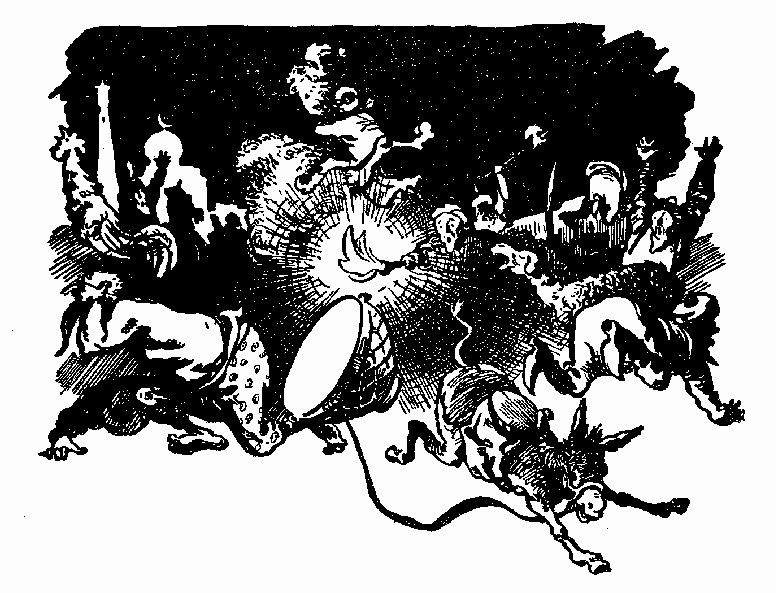
\includegraphics[width=\textwidth]{6.png}
\end{figure}

Через минуту вся площадь и~все прилегающие улицы были охвачены великим ужасом и~небывалым смятением: грохот, звон, гром, ржание, рев, лай, вой, треск и~дребезжание~— все это сливалось в~какой-то адский гул, и~никто не~мог ничего понять; многие сотни верблюдов, лошадей, ишаков, сорвавшихся с~привязи, носились во~мраке, гремя по~разбросанным всюду медным листам, а~погонщики вопили и~метались, размахивая факелами. От~страшного шума люди просыпались, вскакивали и~полуголые бежали, сами не~зная куда, наталкиваясь друг на~друга, оглашая темноту криками отчаяния и~скорби, так как думали, что настал конец света. Заорали и~захлопали крыльями петухи. Смятение росло, охватывая весь огромный город до~самых окраин,~— и~вот ударили пушки на~городской стене, ибо городская стража решила, что в~Бухару ворвался неприятель, и~ударили пушки во~дворце, ибо дворцовая стража решила, что начался бунт; со~всех бесчисленных минаретов понеслись надрывные, тревожные голоса муэдзинов,~— все перемешалось, и~никто не~знал, куда бежать и~что делать! А~в~самой кромешной гуще, ловко увертываясь от~обезумевших лошадей и~верблюдов, бегал Ходжа Насреддин, преследуя по~грохоту барабана своего ишака, но~так и~не~мог поймать, пока не~оборвалась веревка и~барабан не~отлетел в~сторону, под ноги верблюдам, которые ринулись от~него, сокрушая с~треском навесы, сараи, чайханы и~лавки.

Долго~бы пришлось Ходже Насреддину ловить ишака, если~бы они не~столкнулись случайно нос к~носу. Ишак был весь в~мыле и~дрожал.

—~Пойдем, пойдем скорее, здесь что-то чересчур шумно для нас,~— сказал Ходжа Насреддин, утаскивая за~собой ишака. —~Удивительно, что может натворить в~большом городе один маленький ишак, если к~нему привязать барабан! Полюбуйся, что ты~наделал! Правда, ты~спас меня от~стражников, но~я~все-таки жалею бедных жителей Бухары: им~хватит теперь разбираться до~утра. Где~же найти нам тихий, уединенный уголок?

Ходжа Насреддин решил переночевать на~кладбище, справедливо рассудив, что какое~бы ни~поднялось смятение, усопшие все равно не~будут бегать, вопить, кричать и~размахивать факелами.

Так Ходжа Насреддин, возмутитель спокойствия и~сеятель раздоров, закончил, вполне достойно своего титула, первый день пребывания в~родном городе. Привязав к~одному из~надгробий ишака, он~удобно устроился на~могиле и~скоро уснул. А~в~городе еще долго продолжалось смятение~— шум, гул, крики, звон и~пушечная пальба.


\chapter{}

Но~как только забрезжил рассвет, потускнели звезды и~выступили из~темноты неясные очертания предметов~— на~площадь вышли многие сотни метельщиков, мусорщиков, плотников и~глинобитчиков; они дружно взялись за~работу: подняли опрокинутые навесы, починили мосты, заделали проломы в~заборах, собрали все щепки и~черепки,~— и~первые лучи солнца уже не~застали в~Бухаре никаких следов ночного смятения.

И~начался базар.

Когда Ходжа Насреддин, хорошо выспавшийся в~тени могильного памятника, приехал на~площадь, она уже вся гудела, волновалась и~двигалась, затопленная из~конца в~конец разноплеменной, разноязычной, многоцветной толпой. «Дорогу! Дорогу!»~— кричал Ходжа Насреддин, но~даже сам с~трудом различал свой голос в~тысячах других голосов, ибо кричали все: купцы, погонщики, водоносы, цирюльники, бродячие дервиши, нищие, базарные зубодеры, потрясавшие ржавыми и~страшными орудиями своего ремесла. Разноцветные халаты, чалмы, попоны, ковры, китайская речь, арабская, индусская, монгольская и~еще множество всяких наречий~— все это слилось воедино, качалось, двигалось, гудело, и~поднималась пыль, и~замутилось небо, а~на~площадь бесконечными потоками прибывали новые сотни людей, раскладывали товары и~присоединяли свои голоса к~общему реву. Гончары выбивали палочками звонкую дробь на~своих горшках и~хватали прохожих за~полы халатов, уговаривая послушать~и, пленившись чистотою звона, купить; в~чеканном ряду нестерпимо для глаз сияла медь, воздух стонал от~говора маленьких молоточков, которыми мастера выбивали узоры на~подносах и~кувшинах, расхваливая громкими голосами свое искусство и~понося искусство соседей. Ювелиры плавили в~маленьких горнах серебро, тянули золото, шлифовали на~кожаных кругах драгоценные индийские самоцветы, легкий ветер порой доносил сюда густую волну благоуханий из~соседнего ряда, где торговали духами, розовым маслом, амброй, мускусом и~различными пряностями; в~сторону уходил нескончаемый ковровый ряд~— пестрый, узорный, цветистый, разукрашенный персидскими, дамасскими, текинскими коврами, кашгарскими паласами, цветными попонами, дорогими и~дешевыми, для простых коней и~для благородных.

Потом Ходжа Насреддин миновал шелковый ряд, седельный, оружейный и~красильный ряды, невольничий рынок, шерстобитный двор~— и~все это было только началом базара, а~дальше тянулись еще сотни различных рядов; и~чем глубже в~толпу пробивался на~своем ишаке Ходжа Насреддин, тем оглушительнее вопили, кричали, спорили, торговали вокруг; да, это был все тот~же базар, знаменитый и~несравненный бухарский базар, равного которому не~имели в~то~время ни~Дамаск, ни~самый Багдад!

Но~вот ряды кончились, и~глазам Ходжи Насреддина открылся эмирский дворец, обнесенный высокой стеной с~бойницами и~зубчатым верхом. Четыре башни по~углам были искусно облицованы разноцветной мозаикой, над которой долгие годы трудились арабские и~иранские мастера.

Перед воротами дворца раскинулся пестрый табор. В~тени изодранных навесов лежали и~сидели на~камышовых циновках люди, истомленные духотой,~— одинокие и~со~своими семьями; женщины укачивали младенцев, варили пищу в~котлах, штопали рваные халаты и~одеяла; всюду бегали полуголые ребятишки, кричали, дрались и~падали, весьма непочтительно обращая ко~дворцу ту~часть тела, которая неприлична для созерцания. Мужчины спали, или занимались различными домашними делами, или беседовали между собой, усевшись вокруг чайников. «Эге! Да~эти люди живут здесь не~первый день!»~— подумал Ходжа Насреддин.

Его внимание привлекли двое: плешивый и~бородатый. Они, повернувшись спинами друг к~другу, лежали прямо на~голой земле, каждый под своим навесом, а~между ними была привязана к~тополевому колышку белая коза, до~того тощая, что ее~ребра грозили прорвать облезшую шкуру. Она с~жалобным блеянием глодала колышек, объеденный уже до~половины.

Ходжа Насреддин был очень любопытен и~не~мог удержаться от~вопроса:

—~Мир вам, жители Благородной Бухары! Скажите мне, давно~ли вы~перешли в~цыганское сословие?

—~Не~смейся над нами, о~путник! —~ответил бородатый. —~Мы~не~цыгане, мы~такие~же добрые мусульмане, как ты~сам.

—~Почему~же вы~не~сидите дома, если вы~добрые мусульмане? Чего вы~ждете здесь перед дворцом?

—~Мы~ждем справедливого и~многомилостивого суда эмира, нашего владыки, повелителя и~господина, затмевающего своим блеском самое солнце.

—~Так! —~сказал Ходжа Насреддин, не~скрывая насмешки. —~И~давно вы~ждете справедливого и~многомилостивого суда эмира, вашего владыки, повелителя и~господина, затмевающего своим блеском самое солнце?

—~Мы~ждем уже шестую неделю, о~путник! —~вмешался плешивый. —~Вот этот бородатый сутяга, да~покарает его аллах, да~подстелет шайтан свой хвост на~его ложе! —~этот бородатый сутяга~— мой старший брат. Наш отец умер и~оставил нам скромное наследство, мы~разделили все, кроме козы. Пусть эмир рассудит, кому из~нас она должна принадлежать.

—~Но~где~же остальное имущество, доставшееся вам в~наследство?

—~Мы~все обратили в~деньги; ведь сочинителям жалоб надо платить, и~писцам, принимающим жалобы, тоже надо платить, и~стражникам надо платить, и~еще многим.

Плешивый вдруг сорвался с~места, бросился навстречу грязному босому дервишу в~остроконечной шапке и~с~черной выдолбленной тыквой на~боку:

—~Помолись, святой человек! Помолись, чтобы суд окончился в~мою пользу!

Дервиш взял деньги, начал молиться. И~каждый раз, когда он~произносил заключительные слова молитвы, плешивый бросал в~его тыкву новую монету и~заставлял повторять все сызнова.

Бородатый с~беспокойством поднялся, обшарил глазами толпу. После недолгих поисков он~заметил второго дервиша, еще более грязного и~оборванного~и, следовательно, еще более святого. Этот дервиш потребовал непомерные деньги, бородатый начал торговаться, но~дервиш, покопавшись под своей шапкой, достал оттуда целую горсть крупных вшей, и~бородатый, удостоверившись в~его святости, согласился. Поглядывая с~торжеством на~своего младшего брата, он~отсчитал деньги. Дервиш, опустившись на~колени, начал громко молиться, перекрывая своим басом тонкий голос первого дервиша. Тогда плешивый, обеспокоившись, добавил денег своему дервишу, а~бородатый~— своему, и~оба дервиша, стараясь превзойти друг друга, закричали и~завопили так громко, что аллах, наверное, приказал ангелам закрыть окна в~своих чертогах, опасаясь оглохнуть. Коза, обгладывая тополевый колышек, блеяла жалобно и~протяжно.

Плешивый бросил ей~полснопа клевера, но~бородатый закричал:

—~Убери свой грязный, вонючий клевер от~моей козы!

Он~отшвырнул клевер далеко в~сторону и~поставил перед козой горшок с~отрубями.

—~Нет! —~злобно завопил плешивый брат. —~Моя коза не~будет есть твои отруби!

Горшок полетел вслед за~клевером, разбился, отруби перемешались с~дорожной пылью, а~братья в~яростной схватке катались уже по~земле, осыпая друг друга ударами и~проклятиями.

—~Два дурака дерутся, два жулика молятся, а~коза тем временем подохла с~голода,~— сказал, покачав головой. Ходжа Насреддин. —~Эй~вы, добродетельные и~любящие братья, взгляните сюда! Аллах по-своему рассудил ваш спор и~забрал козу себе!

Братья, опомнившись, отпустили друг друга и~долго стояли с~окровавленными лицами, разглядывая издохшую козу. Наконец плешивый сказал:

—~Надо снять шкуру.

—~Я~сниму шкуру! —~быстро отозвался бородатый.

—~Почему~же ты? —~спросил второй; плешь его побагровела от~ярости.

—~Коза моя, значит, и~шкура моя!

—~Нет, моя!

Ходжа Насреддин не~успел вставить слова, как братья опять катались по~земле, и~ничего нельзя было разобрать в~этом хрипящем клубке, только на~мгновение высунулся грязный кулак с~зажатым в~нем пучком черных волос, из~чего Ходжа Насреддин заключил, что старший брат лишился значительной части своей бороды.

Безнадежно махнув рукой. Ходжа Насреддин поехал дальше. Навстречу ему попался кузнец с~клещами за~поясом~— тот самый, с~которым Ходжа Насреддин разговаривал вчера у~водоема.

—~Здравствуй, кузнец! —~радостно закричал Ходжа Насреддин. —~Вот мы~и~встретились, хотя я~и~не~успел еще выполнить своей клятвы. Что ты~здесь делаешь, кузнец, разве и~ты~пришел на~эмирский суд?

—~Только будет~ли польза от~этого суда? —~угрюмо ответил кузнец. —~Я~пришел с~жалобой от~кузнечного ряда. Нам дали пятнадцать стражников, чтобы мы~кормили их~три месяца, но~прошел уже целый год, а~мы~все кормим и~кормим и~терпим большие убытки.

—~А~я~пришел от~красильного ряда,~— вмешался какой-то человек со~следами краски на~руках, с~лицом, позеленевшим от~ядовитых паров, которые вдыхал он~ежедневно от~восхода до~заката. —~Я~принес такую~же точно жалобу. К~нам поставили на~прокормление двадцать пять стражников, торговля наша разрушилась, доходы наши пришли в~упадок. Может быть, эмир смилуется и~освободит нас от~этого нестерпимого ярма.

—~И~за~что только вы~ополчились на~бедных стражников! —~воскликнул Ходжа Насреддин. —~Право~же, они не~самые худшие и~прожорливые среди жителей Бухары. Вы~безропотно кормите самого эмира, всех его визирей и~сановников, кормите две тысячи мулл и~шесть тысяч дервишей,~— почему~же несчастные стражники должны голодать? И~разве не~знаете вы~поговорки: там, где нашел себе пропитание один шакал, сейчас~же заводится еще десяток? Я~не~понимаю вашего недовольства, о~кузнец и~красильщик!

—~Тише! —~сказал кузнец, оглядываясь. Красильщик смотрел на~Ходжу Насреддина с~упреком:

—~Ты~опасный человек, путник, и~слова твои не~добродетельны. Но~эмир наш мудр и~многомилостив...

Он~не~договорил, потому что завыли трубы, ударили барабаны, весь пестрый табор всколыхнулся, пришел в~движение~— и~тяжело открылись окованные медью ворота дворца.

—~Эмир! Эмир! —~понеслись крики, и~народ со~всех концов хлынул ко~дворцу, чтобы взглянуть на~своего повелителя.

Ходжа Насреддин занял самое удобное место в~первых рядах.

Сначала из~ворот выбежали глашатаи:

—~Дорогу эмиру! Дорогу светлейшему эмиру! Дорогу повелителю правоверных!

Следом за~ними выскочила стража, колотя палками направо и~налево, по~головам и~спинам любопытных, придвинувшихся слишком близко; в~толпе образовался широкий проход, и~вышли тогда музыканты с~барабанами, флейтами, бубнами и~карнаями; за~ними следовала свита~— в~шелках и~золоте, с~кривыми саблями в~бархатных ножнах, усыпанных драгоценными камнями; потом провели двух слонов с~высокими султанами на~головах; наконец, вынесли пышно разукрашенные носилки, в~которых под тяжелым парчовым балдахином возлежал сам великий эмир.

Толпа зарокотала, загудела навстречу ему; словно~бы ветер прошел по~всей площади, и~народ распростерся ниц, как этого требовал эмирский указ, повелевавший верноподданным смотреть на~своего владыку с~подобострастием и~обязательно снизу вверх. Перед носилками бежали слуги, расстилая ковры на~пути; справа от~носилок шел дворцовый мухобой с~опахалом из~конских хвостов на~плече, а~слева степенно и~важно шагал эмирский кальянщик с~турецким золотым кальяном в~руках. Шествие замыкала стража в~медных шлемах, со~щитами, копьями, самострелами и~саблями наголо; в~самом хвосте везли две маленькие пушки. Все это освещалось ярким полуденным солнцем,~— оно зажгло драгоценные камни, горело на~золотых и~серебряных украшениях, жарким блеском отражалось в~медных щитах и~шлемах, сияло на~белой стали обнаженных клинков... Но~в~огромной, распростертой ниц толпе не~было ни~драгоценных камней, ни~золота, ни~серебра, ни~даже меди,~— ничего, что могло~бы, радуя сердца, гореть и~сиять под солнцем,~— только лохмотья, нищета, голод; и~когда пышная эмирская процессия двигалась через море грязного, темного, забитого и~оборванного народа, похоже было, что тянут сквозь жалкое рубище тонкую и~единственную золотую нить.

Высокий, устланный коврами помост, откуда надлежало эмиру излить на~преданный ему народ свою милость, был уже оцеплен со~всех сторон стражниками, а~внизу на~лобном месте хлопотали палачи, готовясь к~исполнению эмирской воли: испытывали гибкость прутьев и~крепость палок, вымачивали в~тазах многохвостые сыромятные плети, ставили виселицы, точили топоры и~укрепляли в~земле заостренные колья. Распоряжался начальник дворцовой стражи Арсланбек, прославившийся свирепостью далеко за~пределами Бухары; он~был красен лицом, грузен телом и~черен волосом, борода покрывала всю его грудь и~опускалась на~живот, голос его был подобен верблюжьему реву.

Он~щедро раздавал зуботычины, пинки, но~вдруг весь изогнулся и~задрожал в~подобострастии.

Носилки, плавно колыхаясь, поднялись на~помост, и~эмир, откинув балдахин, явил народу свое лицо.


\chapter{}

Он~был не~очень уж~красив с~виду, пресветлый эмир; лицо его, которое придворные поэты всегда сравнивали в~своих стихах с~полной серебристой луной, гораздо более напоминало перезрелую, вялую дыню. Когда эмир, поддерживаемый визирями, встал с~носилок, чтобы пересесть на~золоченый трон. Ходжа Насреддин убедился, что и~стан его, вопреки единодушному утверждению придворных поэтов, далеко не~подобен стройному кипарису; туловище эмира было тучным и~грузным, руки~— короткими, а~ноги~— столь кривыми, что даже халат не~мог скрыть их~уродства.

Визири заняли свои места с~правой стороны, муллы и~сановники~— с~левой, писцы со~своими книгами и~чернильницами разместились внизу, придворные поэты выстроились полукругом позади трона, глядя в~затылок эмиру преданными глазами. Дворцовый мухобой взмахнул опахалом. Кальянщик сунул в~рот своему господину золотой чубук. Толпа вокруг помоста затаила дыхание. Ходжа Насреддин, приподнявшись в~седле и~вытянув шею, весь обратился в~слух.

Эмир сонно кивнул головой. Стражники расступились, пропуская плешивого и~бородатого, дождавшихся, наконец, своей очереди. Братья подползли на~коленях к~помосту, коснулись губами ковра, свисавшего до~земли.

—~Встаньте! —~приказал великий визирь Бахтияр.

Братья встали, не~осмеливаясь отряхнуть пыль со~своих халатов. Их~языки заплетались от~страха, речь была непонятна и~сбивчива. Но~Бахтияр был многоопытный визирь и~понял все с~полуслова.

—~Где ваша коза? —~нетерпеливо прервал он~братьев.

Плешивый ответил ему:

—~Она умерла, о~высокорожденный визирь! Аллах взял нашу козу к~себе. Но~кому~же из~нас должна теперь принадлежать ее~шкура?

Бахтияр повернулся к~эмиру:

—~Каково будет твое решение, о~мудрейший из~повелителей?

Эмир протяжно зевнул и~с~видом полного безразличия закрыл глаза. Бахтияр почтительно склонил голову, отягощенную белой чалмой:

—~Я~прочел решение на~твоем лице, о~владыка!.. Слушайте,~— обратился он~к~братьям; они опустились на~колени, готовясь поблагодарить эмира за~мудрость, справедливость и~милосердие. Бахтияр объявил приговор; писцы заскрипели перьями, записывая его слова в~толстые книги. —~Повелитель правоверных и~солнце вселенной, наш великий эмир, да~пребудет над ним благословение аллаха, рассудить соизволил, что если козу взял к~себе аллах, то~шкура ее~по~справедливости должна принадлежать наместнику аллаха на~земле, то~есть великому эмиру, для чего надлежит снять с~козы шкуру, высушить и~обработать ее~и~принести во~дворец и~сдать в~казну.

Братья в~растерянности переглянулись, по~толпе пробежал легкий шепот. Бахтияр продолжал раздельно и~громко:

—~Кроме того, надлежит взыскать с~тяжущихся судебную пошлину в~размере двухсот таньга, и~дворцовую пошлину в~размере полутораста таньга, и~налог на~содержание писцов в~размере пятидесяти таньга, и~пожертвование на~украшение мечетей,~— и~все это надлежит взыскать с~них немедленно деньгами, или одеждой, или прочим имуществом.

И~еще не~успел он~закончить, как стражники по~знаку Арсланбека кинулись к~братьям, оттащили в~сторону, развязали их~пояса и~вывернули карманы, сорвали халаты, стащили сапоги и~вытолкали в~шею, босых и~полуголых, едва прикрывающих жалкой одеждой свой срам.

Все это произошло в~полминуты. Сразу~же после объявления приговора весь хор придворных поэтов пришел в~движение и~начал славословие на~разные голоса:

—~О~мудрый эмир, о~мудрейший из~мудрых, о~умудренный мудростью мудрых, о~над мудрыми мудрый эмир!..

Так они восклицали долго, вытягивая шеи по~направлению к~трону; каждый старался, чтобы эмир отличил его голос из~всех других голосов. А~простые люди, толпившиеся вокруг помоста, молчали, с~жалостью глядя на~братьев.

—~Ну~вот,~— заметил благочестивым тоном Ходжа Насреддин, обращаясь к~несчастным, которые громко рыдали в~объятиях друг друга. —~Вы~все-таки не~зря просидели шесть недель на~площади. Наконец-то вы~дождались справедливого и~всемилостивого решения, ибо известно всем, что в~мире нет никого мудрее и~милосерднее нашего эмира, а~если кто-нибудь сомневается в~этом,~— и~он~обвел глазами своих соседей в~толпе,~— то~недолго крикнуть стражников, и~они предадут нечестивца в~руки палачей, и~уж~тем ничего не~стоит разъяснить человеку всю гибельность его заблуждений. Ступайте с~миром домой, о~братья; если впредь у~вас случится спор из-за курицы~— приходите снова на~эмирский суд, но~предварительно не~забудьте продать свои дома, виноградники и~поля, ибо иначе вы~не~сможете уплатить всех пошлин.

—~О, лучше~бы нам умереть вместе с~нашей козой! —~воскликнули братья, роняя крупные слезы.

—~Вы~думаете, там, на~небе, мало своих дураков? —~ответил Ходжа Насреддин. —~Достойные доверия люди говорили мне, что нынче и~ад~и~рай набиты дураками до~отказа~— больше туда не~пускают. Я~предсказываю вам бессмертие, братья, и~уходите скорей отсюда, потому что стражники начали уже поглядывать в~нашу сторону, а~я~не~могу рассчитывать на~бессмертие, подобно вам.

Братья ушли, громко рыдая, царапая лица и~посыпая головы желтой дорожной пылью.

Перед эмирским судом предстал кузнец. Он~изложил глухим и~угрюмым голосом свою жалобу. Великий визирь Бахтияр повернулся к~эмиру:

—~Каково будет твое решение, о~повелитель? Эмир спал, приоткрыв рот и~похрапывая. Но~Бахтияр нисколько не~смутился:

—~О~владыка! Я~читаю решение на~твоем лице! И~торжественно возгласил:

—~Во~имя аллаха милостивого и~милосердного: повелитель правоверных и~наш владыка эмир, в~неустанной заботе о~своих подданных, оказал им~великую милость и~благоволение, поставив на~прокормление к~ним верных стражников его, эмирской, службы, и~тем самым даровал жителям Благородной Бухары почетную возможность возблагодарить своего эмира, и~благодарить его каждодневно и~ежечасно, каковой чести не~удостоено от~своих правителей население иных, сопредельных с~нашим, государств. Однако кузнечный ряд не~отличился благочестием среди прочих. Напротив того: кузнец Юсуп, позабыв о~замогильных страданиях и~волосяном мосту для грешников, дерзко отверз свои уста для выражения неблагодарности, каковую и~осмелился принести к~стопам нашего повелителя и~господина, пресветлого эмира, затмевающего своим блеском самое солнце. Войдя в~рассуждение этого, наш пресветлый эмир рассудить соизволил: даровать кузнецу Юсупу двести плетей, дабы внушить ему слова покаяния, без чего тщетно пришлось~бы ему ожидать, чтобы перед ним открылись райские врата. Всему~же кузнечному ряду пресветлый эмир вновь оказывает снисхождение и~милость и~повелевает поставить еще двадцать стражников на~прокормление, дабы не~лишать кузнецов радостной возможности каждодневно и~ежечасно восхвалять его мудрость и~милосердие. Таково решение эмира, да~продлит аллах его дни на~благо всем верноподданным!

Весь хор придворных льстецов снова пришел в~движение и~загудел на~разные голоса, прославляя эмира. Стража тем временем схватила кузнеца Юсупа и~потащила к~лобному месту, где палачи с~мерзкими кровожадными улыбками уже взвешивали в~руках тяжелые плети.

Кузнец лег ничком на~циновку; свистнула, опустилась плеть, спина кузнеца окрасилась кровью.

Палачи били его жестоко, взлохматили всю кожу на~спине и~просекли до~самых костей мясо, но~так и~не~смогли услышать от~кузнеца не~только вопля, но~хотя~бы стона. Когда он~встал, то~все заметили на~губах его черную пену: он~грыз землю во~время порки, чтобы не~кричать.

—~Этот кузнец не~из~таких, что легко забывают,~— сказал Ходжа Насреддин. —~Он~будет теперь до~конца своих дней помнить эмирскую милость. Чего~же ты~стоишь, красильщик,~— иди, сейчас твоя очередь.

Красильщик плюнул~и, не~оглядываясь, пошел прочь из~толпы.

Великий визирь быстро закончил еще несколько дел, причем из~каждого дела неукоснительно извлекал пользу для эмирской казны, каковым умением и~был он~знаменит среди прочих сановников.

Палачи работали на~лобном месте без передышки. Оттуда неслись вопли и~крики. Великий визирь посылал к~палачам все новых и~новых грешников, и~они уже образовали длинную очередь~— старики, женщины и~даже десятилетний мальчик, изобличенный и~дерзком и~вольнодумном увлажнении земли перед эмирским дворцом. Он~дрожал и~плакал, размазывая слезы по~лицу. Ходжа Насреддин смотрел на~него с~жалостью и~негодованием в~сердце.

—~Поистине, он~опасный преступник, этот мальчик! —~громко рассуждал Ходжа Насреддин. —~И~нельзя достаточно восхвалить предусмотрительность эмира, оберегающего свой трон от~подобных врагов, которые чем более опасны, что прикрывают молодостью лет подозрительное направление своих мыслей. Не~далее как сегодня я~видел еще одного преступника, худшего и~ужаснейшего в~сравнении с~этим. Тот преступник~— ну, что~бы вы~могли подумать? —~он~совершил еще большее под самой стеной дворца! Любое наказание было~бы слишком легким за~подобную дерзость, разве вот посадить его на~кол. Я~только боюсь, что кол прошел~бы через этого преступника насквозь, как вертел через цыпленка, ибо ему, преступнику, исполнилось всего-навсего четыре года. Но~это, конечно, как я~уже говорил, не~может служить оправданием.

Так он~говорил, стараясь походить на~муллу, произносящего проповедь; и~голос его, и~слова были благонамеренны, но~люди, имеющие уши, слышали, понимали и~прятали в~бороды затаенные, недобрые усмешки.


\chapter{}

Вдруг Ходжа Насреддин заметил, что толпа поредела. Многие торопливо расходились, даже разбегались. «Уж~не~подбираются~ли ко~мне стражники?»~— подумал он~с~беспокойством.

Он~сразу все понял, когда увидел приближающегося ростовщика. За~ним, под охраной стражников, шли дряхлый седобородый старик в~халате, перепачканном глиной, и~закутанная в~покрывало женщина, вернее~— девушка, совсем еще молодая, как это установил Ходжа Насреддин, вглядевшись опытным глазом в~ее~походку.

—~А~где~же Закир, Джура, Мухаммед и~Садык? —~спросил скрипучим голосом ростовщик, обводя людей своим единственным оком; второе~же было тускло и~неподвижно, затянутое бельмом. —~Они только что были здесь, я~заметил еще издали. Скоро наступит срок их~долгам, напрасно они бегают и~скрываются. В~нужный день я~все равно их~найду.

Прихрамывая, он~потащил свой горб дальше.

—~Смотрите, смотрите, этот паук повел на~эмирский суд горшечника Нияза и~его дочку!

—~Он~не~дал горшечнику даже одного дня отсрочки!

—~Будь он~проклят, этот ростовщик. Через две недели срок уплаты моего долга!

—~А~мой срок через неделю.

—~Смотрите, все разбегаются перед ним и~прячутся, как будто он~разносит проказу или холеру!

—~Он~хуже прокаженного, этот ростовщик! Душу Ходжи Насреддина терзало горькое раскаяние. Он~повторял свою клятву: «Я~утоплю его в~том~же самом пруду!»

Арсланбек пропустил ростовщика вне очереди. За~ростовщиком к~помосту подошли горшечник и~его дочь, стали на~колени, поцеловали бахрому ковра.

—~Мир тебе, почтенный Джафар! —~приветливо сказал великий визирь. —~Какое дело привело тебя сюда? Изложи свое дело великому эмиру, припадая к~его стопам.

—~О~великий владыка, господин мой! —~начал Джафар, обращаясь к~эмиру, который кивнул сквозь дрему и~опять захрапел и~засвистел носом. —~Я~пришел просить у~тебя справедливости. Вот этот человек, по~имени Нияз и~по~занятиям горшечник, должен мне сто таньга и~еще триста таньга процентов на~этот долг. Сегодня утром наступил срок уплаты, но~горшечник ничего не~уплатил мне. Рассуди нас, о~мудрый эмир, солнце вселенной!

Писцы записали в~книге жалобу ростовщика, после чего великий визирь обратился к~горшечнику:

\begin{figure}[h]
\centering
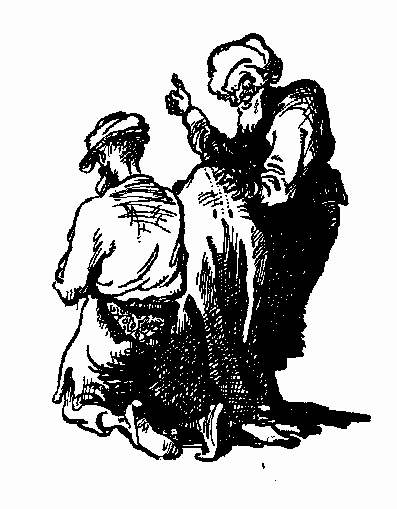
\includegraphics[scale=0.75]{7.png}
\end{figure}

—~Горшечник, тебя спрашивает великий эмир. Признаешь~ли ты~этот долг? Может быть, ты~оспариваешь день и~час?

—~Нет,~— слабым голосом ответил горшечник, и~его седая голова поникла. —~Нет, мудрейший и~справедливейший визирь, я~ничего не~оспариваю~— ни~долга, ни~дня, ни~часа. Я~только прошу отсрочки на~один месяц и~прибегаю к~великодушию и~милости нашего эмира.

—~Позволь, о~владыка, объявить решение, которое я~прочел на~твоем лице,~— сказал Бахтияр. —~Во~имя аллаха милостивого и~милосердного: по~закону, если кто-нибудь не~уплатит в~срок своего долга, то~поступает со~всей семьей в~рабство к~тому, кому должен, и~пребывает в~рабстве до~тех пор, пока не~уплатит долга с~процентами за~все время, включая сюда также и~время, проведенное в~рабстве.

Голова горшечника опускалась все ниже и~вдруг затряслась, многие в~толпе отвернулись, подавляя тяжелые вздохи.

\begin{figure}[h]
\centering
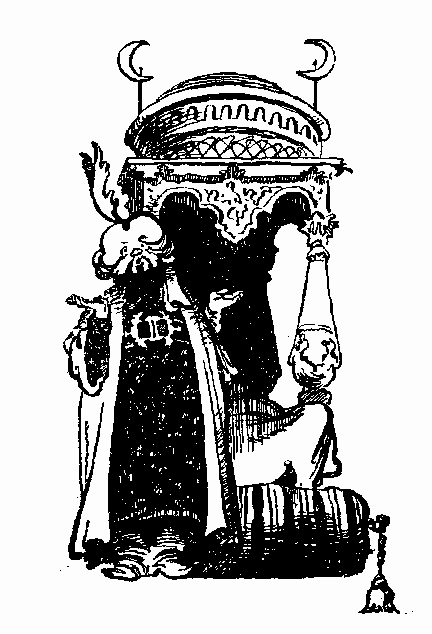
\includegraphics[scale=0.62]{8.png}
\end{figure}

Плечи девушки дрогнули: она плакала под своим покрывалом.

Ходжа Насреддин в~сотый раз повторил про себя:

"Он~будет утоплен, этот безжалостный истязатель бедняков!

—~Но~милость нашего повелителя эмира и~великодушие его безграничны! —~продолжал между тем Бахтияр, возвысив голос. Толпа затихла. Старый горшечник поднял голову, лицо его просветлилось надеждой.

—~Хотя срок уплаты долга уже миновал, но~эмир дарует горшечнику Ниязу отсрочку~— один час. Если~же по~истечении этого часа горшечник Нияз пренебрежет установлениями веры и~не~уплатит всего долга с~процентами, следует поступить по~закону, как уже было сказано. Иди, горшечник, и~да~пребудет над тобою впредь милость эмира.

Бахтияр умолк, и~тогда пришел в~движение и~загудел хор льстецов, толпившихся позади трона:

—~О~справедливый, затмевающий своей справедливостью самую справедливость, о~милосердный и~мудрый, о~великодушный эмир, о~украшение земли и~слава неба, наш пресветлый эмир!

На~этот раз льстецы превзошли самих себя и~славословили столь громко, что даже разбудили эмира, который, недовольно поморщившись, приказал им~замолчать. Они умолкли, и~весь народ на~площади молчал, и~вдруг в~этой тишине раздался могучий, терзающий уши рев.

Это ревел ишак Ходжи Насреддина. То~ли наскучило ему стоять на~одном месте, то~ли заметил он~где-нибудь длинноухого собрата и~решил с~ним поздороваться, но~он~ревел, приподняв хвост, вытянув морду с~желтыми оскаленными зубами, ревел оглушительно, неудержимо, и~если останавливался на~мгновение, то~затем только, чтобы, передохнув, открыть свою пасть еще шире и~зареветь, заскрипеть еще громче.

Эмир заткнул уши. Стражники бросились в~толпу. Но~Ходжа Насреддин был уже далеко. Он~тащил упиравшегося ишака и~во~всеуслышание ругал его:

—~Чему ты~обрадовался, проклятый ишак! Неужели ты~не~можешь потише восхвалять милосердие и~мудрость эмира! Или, может быть, ты~надеешься получить за~свое усердие должность главного придворного льстеца?

Толпа громким хохотом встречала его слова, расступалась перед ним и~опять смыкалась перед стражниками, которым так и~не~удалось догнать Ходжу Насреддина, положить его за~дерзкое возмущение спокойствия под плети и~отобрать в~эмирскую казну ишака.


\chapter{}

—~Ну~вот, суд закончился, и~теперь моя власть над вами безгранична,~— говорил ростовщик Джафар горшечнику Ниязу и~его дочке Гюльджан, когда после объявления приговора они втроем покинули место судилища. —~Красавица, с~тех пор как я~случайно увидел тебя, я~лишился сна и~покоя. Покажи мне свое лицо. Сегодня, ровно через час, ты~войдешь в~мой дом. И~если ты~будешь благосклонна ко~мне~— я~дам твоему отцу легкую работу и~хорошую пищу; если~же ты~будешь упрямиться, тогда, клянусь светом очей моих, я~буду кормить его сырыми бобами, заставлю таскать камни и~продам хивинцам, жестокость которых в~обращении с~невольниками общеизвестна. Не~упрямься~же и~покажи мне свое лицо, о~прекрасная Гюльджан!

Сладострастными, крючковатыми пальцами он~приподнял ее~покрывало. Гневным движением она отбросила его руку. Лицо Гюльджан оставалось открытым только одно мгновение, но~и~этого было достаточно, чтобы Ходжа Насреддин, проезжавший мимо на~своем ишаке, успел подсмотреть. И~красота девушки была столь удивительной и~необычайной, что Ходжа Насреддин едва не~лишился чувств: мир померк перед его глазами, сердце перестало биться~— он~побледнел, покачнулся в~седле~и, потрясенный, закрыл ладонью глаза. Любовь сразила его мгновенно, подобно молнии.~/ Прошло немало времени, прежде чем он~опомнился.

—~И~эта хромая, горбатая, кривая обезьяна осмеливается посягать на~такую еще не~бывалую в~мире красоту! —~воскликнул~он. —~Зачем, зачем я~вытащил его вчера из~воды; и~вот мое дело уже обратилось против меня! Но~посмотрим, посмотрим еще, грязный ростовщик! Ты~еще не~хозяин над горшечником и~его дочерью, они имеют еще целый час отсрочки, а~Ходжа Насреддин за~один час может сделать столько, сколько другой человек не~сделает за~целый год!

Между тем ростовщик, достав из~своей сумки солнечные деревянные часы, отметил время:

—~Жди меня здесь, горшечник, под этим деревом. Я~вернусь через час, и~не~пытайся скрыться, ибо я~все равно разыщу тебя даже на~дне морском и~поступлю с~тобой, как с~бежавшим невольником. А~ты, прекрасная Гюльджан, подумай над моими словами: от~твоей благодарности зависит теперь судьба твоего отца.

И~с~торжествующей усмешкой на~своей гнусной роже он~отправился в~ювелирный ряд за~украшениями для новой наложницы.

Горшечник, согбенный горем, и~дочка его остались в~тени придорожного дерева. Подошел Ходжа Насреддин:

—~Горшечник, я~слышал приговор. Тебя постигла беда, но, может быть, я~сумею помочь тебе?

—~Нет, добрый человек,~— ответил горшечник с~отчаянием в~голосе. —~Я~вижу по~твоим заплатам, что ты~не~обладаешь богатством. Мне ведь нужно достать целых четыреста таньга! У~меня нет таких богатых знакомых, все мои друзья бедны, разорены поборами и~налогами.

—~У~меня тоже нет богатых друзей в~Бухаре, но~я~все-таки попробую достать деньги,~— перебил Ходжа Насреддин.

—~Достать за~один час четыреста таньга! —~Старик с~горькой усмешкой покачал седой головой. —~Ты, наверное, смеешься надо мной, прохожий! В~подобном деле мог~бы достичь успеха разве только Ходжа Насреддин.

—~О~прохожий, спаси нас, спаси! —~воскликнула Гюльджан, обнимая отца. Ходжа Насреддин взглянул на~нее и~увидел, что кисти рук ее~совершенны; она ответила ему долгим взглядом, он~уловил сквозь чадру влажный блеск ее~глаз, полных мольбы и~надежды. Кровь его вскипела, пробежала огнем по~жилам, любовь его усилилась многократно. Он~сказал горшечнику:

—~Сиди здесь, старик, и~жди меня, и~пусть я~буду самым презренным и~последним из~людей, если не~достану до~прихода ростовщика четырехсот таньга!

Вскочив на~ишака, он~исчез в~базарной толпе...


\chapter{}

На~площади было гораздо тише и~просторнее, чем утром, в~часы торговой горячки, когда все бежали, кричали, спешили, боясь прозевать свою удачу. Близился полдень, и~народ, спасаясь от~зноя, расходился по~чайханам, чтобы спокойно подсчитать прибыли и~убытки. Солнце заливало площадь жарким светом, тени были короткими, резкими, словно высеченными в~жесткой земле. В~затененных местах всюду приютились нищие, а~около них прыгали с~веселым чириканьем воробьи, подбирая крошки.

—~Подай, добрый человек, во~имя аллаха! —~гнусавили нищие, показывая Ходже Насреддину свои уродства и~язвы.

Он~отвечал сердито:

—~Уберите свои руки. Я~ничуть не~богаче вас и~сам ищу, кто~бы дал мне четыреста таньга.

Нищие, принимая эти слова за~насмешку, осыпали Ходжу Насреддина руганью. Он~не~отвечал, погрузившись в~раздумье.

Он~выбрал в~ряду чайхан самую большую и~людную, где не~было ни~дорогих ковров, ни~шелковых подушек, вошел и~втащил за~собой по~ступенькам лестницы ишака, вместо того чтобы поставить у~коновязи.

Ходжу Насреддина встретили удивленным молчанием, но~он~ничуть не~смутился, достал из~переметной сумки коран, что подарил ему вчера на~прощание старик, и, раскрыв, положил перед ишаком.

Все это он~проделал неторопливо и~спокойно, без улыбки на~лице, как будто так и~полагалось.

Люди в~чайхане начали переглядываться. Ишак стукнул копытом в~деревянный гулкий настил.

—~Уже? —~спросил Ходжа Насреддин и~перевернул страницу. —~Ты~делаешь заметные успехи.

Тогда встал со~своего места пузатый добродушный чайханщик и~подошел к~Ходже Насреддину:

—~Послушай, добрый человек, разве здесь место для твоего ишака? И~зачем ты~положил перед ним священную книгу?

—~Я~учу этого ишака богословию,~— невозмутимо ответил Ходжа Насреддин. —~Мы~уже заканчиваем коран и~скоро перейдем к~шариату.

По~чайхане пошел гул и~шепот, многие встали, чтобы лучше видеть.

Глаза чайханщика округлились, рот приоткрылся. Еще никогда в~жизни ему не~приходилось видеть такого чуда. В~это время ишак снова стукнул копытом.

—~Хорошо,~— похвалил Ходжа Насреддин, переворачивая страницу. —~Очень хорошо! Еще немного усилий, и~ты~сможешь занять должность главного богослова в~медресе Мир-Араб. Вот только страницы он~не~умеет перелистывать сам, приходится ему помогать... Аллах снабдил его острым умом и~замечательной памятью, но~позабыл снабдить его пальцами,~— добавил Ходжа Насреддин, обратившись к~чайханщику.

Люди в~чайхане, побросав свои чайники, подошли ближе; не~прошло и~минуты, как вокруг Ходжи Насреддина собралась толпа.

—~Этот ишак~— не~простой ишак! —~объявил Насреддин. —~Он~принадлежит самому эмиру. Однажды эмир позвал меня и~спросил: «Можешь~ли ты~обучить моего любимого ишака богословию, чтобы он~знал столько~же, сколько я~сам?» Мне показали ишака, я~проверил его способности и~ответил: «О~пресветлый эмир! Этот замечательный ишак не~уступает остротой своего ума ни~одному из~твоих министров, ни~даже тебе самому, я~берусь обучить его богословию, и~он~будет знать столько~же, сколько знаешь~ты, и~даже больше, но~для этого потребуется двадцать лет». Эмир велел выдать мне из~казны пять тысяч таньга золотом и~сказал: «Бери этого ишака и~учи его, но, клянусь аллахом, если через двадцать лет он~не~будет знать богословия и~читать наизусть коран, я~отрублю тебе голову!»

—~Ну, значит, ты~заранее можешь проститься со~своей головой! —~воскликнул чайханщик. —~Да~где~же это видано, чтобы ишаки учились богословию и~наизусть читали коран!

—~Таких ишаков немало и~сейчас в~Бухаре,~— ответил Ходжа Насреддин. —~Скажу еще, что получить пять тысяч таньга золотом и~хорошего ишака в~хозяйство~— это человеку не~каждый день удается. А~голову мою не~оплакивай, потому что за~двадцать лет кто-нибудь из~нас уж~обязательно умрет~— или~я, или эмир, или этот ишак. А~тогда поди разбирайся, кто из~нас троих лучше знал богословие!

Чайхана едва не~обрушилась от~взрыва громового хохота, а~сам чайханщик повалился в~корчах на~кошму и~смеялся так, что все лицо его было мокрым от~слез. Он~был очень веселый и~смешливый человек, этот чайханщик!

—~Вы~слышали! —~кричал~он, хрипя и~задыхаясь. —~Тогда пусть разбираются, кто из~них лучше знал богословие! —~И, наверное, он~лопнул~бы от~смеха, если~бы вдруг не~осенила его догадка.

—~Подождите! Подождите! —~Он~замахал руками, призывая всех к~вниманию. —~Кто ты~и~откуда, о~человек, обучающий богословию своего ишака? Да~ты~уж~не~сам~ли Ходжа Насреддин?

—~А~что~же удивительного в~этом? Ты~угадал, чайханщик! Я~— Ходжа Насреддин. Здравствуйте, жители Благородной Бухары!

Было всеобщее оцепенение, и~длилось оно долго; вдруг чей-то ликующий голос прорвал тишину:

—~Ходжа Насреддин!

—~Ходжа Насреддин! —~подхватил второй, за~ним~— третий, четвертый; и~пошло по~чайхане, по~другим чайханам, по~всему базару,~— везде гудело, повторялось и~отдавалось:

—~Ходжа Насреддин! Ходжа Насреддин!

Люди бежали со~всех концов к~чайхане~— узбеки, таджики, иранцы, туркмены, арабы, турки, грузины, армяне, татары~— и, добежав, громкими криками приветствовали своего любимца, знаменитого хитреца и~весельчака Ходжу Насреддина.

Толпа все увеличивалась.

Перед ишаком откуда-то появилась торба с~овсом, сноп клевера, ведро чистой холодной воды.

—~Привет тебе. Ходжа Насреддин! —~неслись крики. —~Где ты~странствовал? Скажи нам что-нибудь, Ходжа Насреддин!

Он~подошел к~самому краю помоста, низко поклонился народу:

—~Приветствую вас, жители Бухары! Десять лет я~был в~разлуке с~вами, и~теперь мое сердце радуется встрече. Вы~просите меня сказать что-нибудь,~— я~лучше спою!

Он~схватил большой глиняный горшок, выплеснул воду~и, ударяя в~него кулаком, как в~бубен, громко запел:

\begin{verse}
Звени, горшок, и~пой, горшок, \\
Достойно восхвали кумира! \\
Поведай миру, о~горшок, \\
О~славных милостях эмира! \\
Горшок звенит, гудит, и~вот \\
Он~гневным голосом поет! \\
Он~хриплым голосом поет, \\
Народ со~всех концов зовет! \\
Послушайте его рассказ: \\
<<Горшечник старый жил~— Нияз, \\
Он~глину мял, горшки лепил, \\
И~он, конечно, беден был, \\
И~денег~— маленький горшок --- \\
За~долгий век скопить не~мог. \\
Зато горбун Джафар не~спит, \\ 
Горшки огромные хранит; \\
Зато эмирская казна \\
Доверху золотом полна, --- \\
И~стража во~дворце не~спит, \\
Горшки огромные хранит. \\
Но~вот беда пришла, как вор, \\
К~Ниязу старому во~двор. \\
Его схватили и~ведут \\
На~площадь, на~эмирский суд. \\
А~сзади, с~видом палача, \\
Идет Джафар, свой горб влача!>> \\
Доколь неправду нам терпеть? \\
Горшок, скажи, горшок, ответь! \\
Правдив твой глиняный язык, \\
Скажи, в~чем виноват старик? \\
Горшок поет, горшок звенит, \\
Горшок правдиво говорит: \\
<<Старик виновен потому, \\
Что в~сеть пришлось попасть ему. \\
И~паутина паука \\
Закабалила старика!>> \\
Пришел на~суд в~слезах старик, \\
К~ногам эмира он~приник. \\
Он~говорит: <<Весь знает мир, \\
Как добр и~благостен эмир, \\
Так пусть~же милости его \\
Коснутся сердца моего!>> \\
Эмир сказал: <<Не~плачь, Нияз, \\
Даю тебе отсрочки... час! \\
Недаром знает целый мир, \\
Как добр и~благостен эмир!>> \\
Доколь неправду нам терпеть? \\
Горшок, скажи, горшок, ответь! \\
Горшок поет, горшок звенит, \\
Горшок правдиво говорит: \\
<<Безумному подобен тот, \\
Кто от~эмира правды ждет. \\
Эмирским милостям цена \\
Всегда одна, всегда одна! \\
Эмир~— он~что? С~дерьмом мешок, \\
И~вместо головы~— горшок!>> \\
Горшок, скажи, горшок, ответь! \\
Доколь эмира нам терпеть? \\
Когда~ж измученный народ \\
Покой и~счастье обретет? \\
Горшок поет, горшок звенит, \\
Горшок правдиво говорит: \\
<<Крепка, сильна эмира власть, \\
Но~и~ему придется пасть. \\
Исчезнут дни твоей тоски. \\
Идут года. И~в~должный срок \\
Он~разлетится на~куски, \\
Как этот глиняный горшок!>>
\end{verse}

Ходжа Насреддин поднял горшок высоко над головой~и, швырнув, ударил сильно об~землю; горшок звонко лопнул, разлетелся на~сотни мелких осколков. Напрягаясь и~перекрывая голосом шум толпы. Ходжа Насреддин закричал:

—~Так давайте вместе спасать горшечника Нияза от~ростовщика и~от~эмирских милостей. Вы~знаете Ходжу Насреддина, за~ним долги не~пропадают! Кто одолжит мне на~короткий срок четыреста таньга?

Вперед выступил босой водонос:

—~Ходжа Насреддин, откуда у~нас деньги? Ведь мы~платим большие налоги. Но~вот у~меня есть пояс, совсем почти новый; за~него можно что-нибудь выручить.

Он~бросил на~помост к~ногам Ходжи Насреддина свой пояс; гул и~движение в~толпе усилились, к~ногам Ходжи Насреддина полетели тюбетейки, туфли, пояса, платки и~даже халаты. Каждый считал честью для себя услужить Ходже Насреддину. Толстый чайханщик принес два самых красивых чайника, медный поднос и~посмотрел на~остальных с~гордостью, ибо пожертвовал щедро. Куча вещей все росла и~росла. Ходжа Насреддин кричал, надрываясь:

—~Довольно, довольно, о~щедрые жители Бухары! Довольно, слышите~ли вы. Седельник, возьми обратно свое седло,~— довольно, говорю~я! Вы~что~— решили превратить Ходжу Насреддина в~старьевщика? Я~начинаю продажу! Вот пояс водоноса, кто купит его, тот никогда не~будет испытывать жажды. Подходите, продаю дешево! Вот старые заплатанные туфли, они уже, наверное, побывали раза два в~Мекке; тот, кто наденет~их, как~бы совершит паломничество! Есть ножи, тюбетейки, халаты, туфли! Берите, я~продаю дешево и~не~торгуюсь, ибо время сейчас для меня дороже всего!

Но~великий Бахтияр, в~неусыпной заботе о~верноподданных, постарался навести в~Бухаре такие порядки, что ни~один грош не~мог задержаться в~карманах жителей и~переходил немедленно в~эмирскую казну,~— дабы жителям легче было ходить с~неотягощенными карманами. Тщетно кричал Ходжа Насреддин, восхваляя свой товар,~— покупателей не~было.


\chapter{}

В~это время неподалеку проходил ростовщик Джафар, его сумку оттягивали золотые и~серебряные украшения, купленные в~ювелирном ряду для Гюльджан.

Хотя час отсрочки был уже на~исходе и~ростовщик спешил, охваченный сластолюбивым нетерпением, но~алчность превозмогла в~нем все другие чувства, когда он~услышал голос Ходжи Насреддина, объявлявшего дешевую распродажу.

Ростовщик приблизился, его заметили, и~толпа начала быстро редеть, ибо каждый третий человек из~собравшихся был должен ему.

Ростовщик узнал Ходжу Насреддина:

—~Это, кажется, ты~здесь торгуешь, человек, вытащивший меня вчера из~воды? Но~откуда у~тебя столько товара?

—~Ты~ведь сам дал мне вчера полтаньга, о~почтенный Джафар,~— ответил Ходжа Насреддин. —~Я~пустил в~оборот эти деньги, и~удача сопутствовала мне в~торговле.

—~Ты~сумел наторговать такую кучу товара за~одно утро? —~воскликнул ростовщик с~удивлением. —~Мои деньги пошли на~пользу тебе. Сколько~же ты~хочешь за~всю эту кучу?

—~Шестьсот таньга.

—~Ты~сошел с~ума! И~тебе не~стыдно заламывать такую цену со~своего благодетеля! Разве не~мне обязан ты~своим благополучием? Двести таньга~— вот моя цена.

—~Пятьсот,~— ответил Ходжа Насреддин. —~Из~уважения к~тебе, почтенный Джафар,~— пятьсот таньга!

—~Неблагодарный! Разве не~мне, повторяю, обязан ты~своим благополучием?

—~А~разве не~мне обязан~ты, ростовщик, своей жизнью? —~ответил Ходжа Насреддин, потеряв терпение. —~Правда, ты~дал мне за~спасение своей жизни всего полтаньга, но~она, твоя жизнь, и~не~стоит большего, я~не~в~обиде! Если ты~хочешь купить, то~говори настоящую цену!

—~Триста!

Ходжа Насреддин молчал.

Ростовщик долго копался, оценивая опытным глазом товар, и, когда убедился, что за~все эти халаты, туфли и~тюбетейки можно выручить самое меньшее семьсот таньга, решил накинуть:

—~Триста пятьдесят.

—~Четыреста.

—~Триста семьдесят пять.

—~Четыреста.

Ходжа Насреддин был непоколебим. Ростовщик уходил и~опять возвращался, накидывая по~одной таньга, наконец согласился. Они ударили по~рукам. Ростовщик с~причитаниями и~стонами начал отсчитывать деньги:

—~Клянусь аллахом, я~переплатил вдвое за~этот товар. Но~такой уж~у~меня характер, что я~всегда терплю большие убытки по~собственной доброте.

—~Фальшивая,~— перебил Ходжа Насреддин, возвращая монету. —~И~здесь не~четыреста таньга. Здесь триста восемьдесят, у~тебя плохое зрение, почтенный Джафар.

Ростовщику пришлось добавить двадцать таньга и~заменить фальшивую монету. Потом он~за~четверть таньга нанял носильщика~и, нагрузив его, приказал следовать за~собой. Бедный носильщик согнулся в~три погибели и~едва не~падал под тяжестью ноши.

—~Нам по~дороге,~— сказал Ходжа Насреддин. Ему не~терпелось увидеть поскорее Гюльджан, и~он~все время прибавлял шагу. Ростовщик со~своей хромой ногой отставал и~шел позади.

—~Куда ты~так спешишь? —~спросил ростовщик, вытирая пот рукавом халата.

—~Туда~же, куда и~ты,~— ответил Ходжа Насреддин, в~его черных глазах блеснули лукавые искры. —~Мы~с~тобой, почтенный Джафар, идем в~одно и~то~же место и~по~одному и~тому~же делу.

—~Но~ты~не~знаешь моего дела,~— сказал ростовщик. —~Если~бы ты~знал, ты~бы мне позавидовал.

Ходже Насреддину был ясен скрытый смысл этих слов, и~он~ответил с~веселым смехом:

—~Но~если~бы ты, ростовщик, знал мое дело, ты~позавидовал~бы мне в~десять раз больше.

Ростовщик насупился: он~уловил дерзость в~ответе Ходжи Насреддина.

—~Ты~невоздержан на~язык; подобный тебе должен трепетать, разговаривая с~подобным мне. Не~много найдется людей в~Бухаре, которым~бы я~завидовал. Я~богат, и~желаниям моим нет преграды. Я~пожелал самую прекрасную девушку в~Бухаре, и~сегодня она будет моей.

В~это время навстречу им~попался продавец вишен с~плоской корзиной на~голове. Ходжа Насреддин мимоходом взял из~корзины одну вишню на~длинном черенке и~показал ее~ростовщику:

—~Выслушай меня, почтенный Джафар. Рассказывают, однажды шакал увидел высоко на~дереве вишню. И~он~сказал себе: «Во~что~бы то~ни~стало, но~я~съем эту вишню». И. он~полез на~дерево, лез туда два часа и~весь ободрался о~сучья. И~когда он~уже приготовился полакомиться и~широко разинул свою пасть~— откуда-то налетел вдруг сокол, схватил вишню и~унес. И~потом шакал спускался на~землю с~дерева опять два часа, ободрался еще больше~и, обливаясь горькими слезами, говорил: «Зачем я~только полез за~этой вишней, ибо давно всем известно, что вишни растут на~деревьях не~для шакалов».

\begin{figure}[h]
\centering
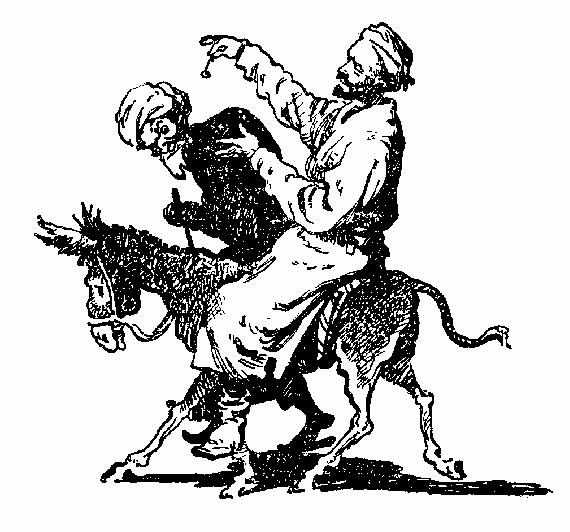
\includegraphics[width=\textwidth]{9.png}
\end{figure}

—~Ты~глуп,~— высокомерно сказал ростовщик. —~В~твоей сказке я~не~вижу смысла.

—~Глубокий смысл познается не~сразу,~— ответил ему Ходжа Насреддин.

Вишня висела у~него за~ухом, черенок ее~был засунут под тюбетейку. Дорога повернула. За~поворотом сидели на~камнях горшечник и~его дочь.

Горшечник встал; глаза его, в~которых все еще светилась надежда, погасли. Он~решил, что чужеземцу не~удалось достать денег. Гюльджан отвернулась с~коротким стоном.

—~Отец, мы~погибли! —~сказала она, и~в~ее~голосе было столько страдания, что даже камень уронил~бы слезу, но~сердце ростовщика было жестче любого камня. Ничего, кроме злобного торжества и~сластолюбия, не~выражалось на~его лице, когда он~сказал:

—~Горшечник, время истекло. Отныне ты~мой невольник, а~дочь твоя~— рабыня и~наложница.

Ему захотелось уязвить и~унизить Ходжу Насреддина, он~властно, по-хозяйски открыл лицо девушки:

—~Посмотри, разве она не~прекрасна? Сегодня я~буду спать с~нею. Скажи теперь, кто кому должен завидовать?

—~Она действительно прекрасна! —~сказал Ходжа Насреддин. —~Но~есть~ли у~тебя расписка горшечника?

—~Конечно. Разве можно вести денежные дела без расписок: ведь все люди~— мошенники и~воры. Вот расписка, здесь обозначен и~долг, и~срок уплаты, горшечник отпечатал внизу свой палец.

Он~протянул расписку Ходже Насреддину.

—~Расписка правильная,~— подтвердил Ходжа Насреддин. —~Получи~же свои деньги по~этой расписке. Остановитесь на~одну минуту, почтенные! Будьте свидетелями,~— добавил~он, обращаясь к~людям, проходившим мимо по~дороге.

Он~разорвал расписку пополам, еще четыре раза пополам и~пустил обрывки по~ветру. Потом он~развязал свой пояс и~вернул ростовщику все деньги, только что полученные от~него~же.

Горшечник и~его дочь окаменели от~неожиданности и~счастья, а~ростовщик от~злобы. Свидетели перемигивались, радуясь посрамлению ненавистного ростовщика.

Ходжа Насреддин взял вишню, опустил ее~в~рот~и, подмигнув ростовщику, громко причмокнул губами.

По~уродливому телу ростовщика прошла медленная судорога, руки скрючились, единственное око злобно вращалось, горб задрожал.

Горшечник и~Гюльджан просили Ходжу Насреддина:

—~О~прохожий, скажи нам свое имя, чтобы мы~знали, за~кого возносить нам молитвы!

—~Да! —~вторил ростовщик, брызгаясь слюной. —~Скажи свое имя, чтобы я~знал, кого проклинать!

Лицо Ходжи Насреддина светилось, он~ответил звонким и~твердым голосом:

—~В~Багдаде и~в~Тегеране, в~Стамбуле и~в~Бухаре~— всюду зовут меня одним именем~— Ходжа Насреддин!

Ростовщик отшатнулся, побелел:

—~Ходжа Насреддин!

И~в~ужасе кинулся прочь, подталкивая в~спину своего носильщика.

Все~же остальные кричали приветственно:

—~Ходжа Насреддин! Ходжа Насреддин! Глаза Гюльджан сияли под чадрой; горшечник все еще не~мог опомниться и~поверить в~свое спасение,~— он~что-то бормотал, разводя в~растерянности руками.


\chapter{}

Эмирский суд продолжался. Палачи сменились несколько раз. Очередь ожидающих порки все увеличивалась. Двое осужденных корчились на~кольях, один лежал обезглавленный на~темной от~крови земле. Но~стоны и~крики не~достигали слуха дремлющего эмира, заглушаемые хором придворных льстецов, охрипших от~усердия. В~своих похвалах они не~забывали великого визиря и~других министров, и~Арсланбека, и~мухобоя, и~кальянщика, справедливо полагая, что угождать надо на~всякий случай всем: одним~— чтобы получить для себя пользу, другим~— чтобы не~причинили вреда.

Арсланбек давно с~беспокойством прислушивался к~странному гулу, доносившемуся издалека.

Он~подозвал двух самых искусных и~опытных шпионов:

—~Идите и~разузнайте, почему волнуется народ. Возвращайтесь немедля.

Шпионы ушли, один~— переодетый в~нищенские лохмотья, второй~— в~одежде странствующего дервиша.

Но~раньше чем вернулись шпионы, прибежал, спотыкаясь и~путаясь в~полах своего халата, бледный ростовщик.

—~Что случилось, почтенный Джафар? —~спросил Арсланбек, меняясь в~лице.

—~Беда! —~ответил трясущимися губами ростовщик. —~О~достопочтенный Арсланбек, случилась большая беда. В~нашем городе появился Ходжа Насреддин. Я~только что видел его и~говорил с~ним.

Глаза Арсланбека выкатились из~орбит и~замерли. Прогибая своей грузностью ступени лестницы, он~вбежал на~помост, пригнулся к~уху дремлющего эмира.

Эмир вдруг подпрыгнул на~троне так высоко, словно его ткнули шилом пониже спины.

—~Ты~лжешь! —~закричал~он, и~лицо его исказилось страхом и~яростью. —~Этого не~может быть! Калиф багдадский недавно писал мне, что отрубил ему голову! Султан турецкий писал, что посадил его на~кол! Шах иранский собственноручно писал мне, что повесил его. Хан хивинский еще в~прошлом году во~всеуслышание объявил, что содрал с~него кожу! Не~мог~же он~в~самом деле уйти невредимым из~рук четырех государей, этот проклятый Ходжа Насреддин!

Визири и~сановники побледнели, услышав имя Ходжи Насреддина. Мухобой, вздрогнув, уронил свое опахало, кальянщик поперхнулся дымом и~закашлялся; льстивые языки поэтов присохли к~зубам от~страха.

—~Он~здесь! —~повторил Арсланбек.

—~Ты~врешь! —~вскричал эмир и~царственной дланью влепил Арсланбеку увесистую пощечину. —~Ты~врешь! А~если он~действительно здесь, то~как он~мог проникнуть в~Бухару, и~куда годится вся твоя стража! Это~он, значит, устроил на~базаре такой переполох сегодня ночью! Он~хотел взбунтовать народ против меня, а~ты~спал и~ничего не~слышал! И~эмир влепил Арсланбеку вторую пощечину. Арсланбек низко поклонился, чмокнул на~лету эмирскую руку:

—~О~повелитель, он~здесь, в~Бухаре. Разве ты~не~слышишь?

Далекий гул усиливался и~нарастал, подобно надвигающемуся землетрясению, и~вот толпа вокруг судилища, захваченная общим волнением, тоже начала гудеть, сначала неясно и~глухо, а~потом все громче, сильнее, и~эмир почувствовал зыбкое колебание помоста и~своего раззолоченного трона. В~эту минуту из~общего слитного гула, переходившего уже в~мощный рев, вдруг всплыло, и~повторилось, и~отдалось многократно во~всех концах:

—~Ходжа Насреддин! Ходжа Насреддин! Стража бросилась с~дымящимися фитилями к~пушкам. Лицо эмира перекосилось от~волнения.

—~Кончайте! —~закричал~он. —~Во~дворец! Подобрав полы парчового халата, он~кинулся во~дворец; за~ним, спотыкаясь, бежали слуги с~пустыми носилками на~плечах. И, объятые смятением, мчались, толкаясь и~обгоняя друг друга, теряя туфли и~не~останавливаясь, чтобы подобрать~их, визири, палачи, музыканты, стражники, мухобой и~кальянщик. Только слоны прошествовали с~прежней важностью и~неторопливостью, ибо они хотя и~числились в~эмир-ской свите, но~не~имели никаких причин бояться народа.

Тяжелые, окованные медью ворота дворца закрылись, пропустив эмира и~его свиту.

А~базарная площадь, затопленная народом, гудела, шумела и~волновалась, повторяя все снова и~снова имя Ходжи Насреддина.


\part{}

\begin{quote}
Вот любопытные происшествия; часть их~случилась в~моем присутствии, а~часть рассказали мне люди, которым я~доверяю.
\flushright{\textit{У~сама ибн Мункыз, «Книга назидания»}}
\end{quote}

\chapter{}

С~незапамятных времен бухарские гончары селились у~восточных ворот вокруг большого глиняного бугра,~— и~не~смогли~бы выбрать лучшего места: глина была здесь рядом, а~водой в~изобилии снабжал их~арык, протекавший вдоль городской стены. Деды, прадеды и~прапрадеды гончаров срыли бугор уже до~половины: из~глины строили они свои дома, из~глины лепили горшки и~в~глину ложились, сопровождаемые горестными воплями родственников; и~потом, через много лет, не~раз, наверное, случалось, что какой-нибудь гончар, вылепив горшок или кувшин, и~высушив на~солнце, и~обработав огнем, дивился небывалому по~силе и~чистоте звону горшка и~не~подозревал, что это далекий предок, заботясь о~благосостоянии потомка и~о~сбыте его товара, облагородил глину частицей своего праха и~заставил ее~звенеть подобно чистому серебру.

Здесь~же стоял и~дом горшечника Нияза~— над самым арыком, в~тени могучих древних карагачей; шелестела под ветром листва, журчала вода, и~с~утра до~вечера слышались в~маленьком садике песни прекрасной Гюльджан.

Ходжа Насреддин отказался поселиться в~доме Нияза:

—~Меня могут схватить в~твоем доме, Нияз. Я~буду ночевать неподалеку, я~нашел тут одно безопасное место. А~днем я~буду приходить сюда и~помогать тебе в~работе.

Так он~и~делал: каждое утро еще до~солнца он~приходил к~Ниязу и~садился вместе со~стариком за~гончарный станок. В~мире не~было ремесла, которого~бы не~знал Ходжа Насреддин; гончарное ремесло знал он~отлично, горшки получались у~него звонкие, гладкие и~обладали способностью сохранять воду ледяной даже в~самую сильную жару. Раньше старик, которому в~последние годы все чаще и~чаще изменяли глаза, едва успевал сделать за~день пять или шесть горшков, а~теперь вдоль забора всегда сушились на~солнцепеке длинные ряды~— тридцать, сорок, а~часто пятьдесят горшков и~кувшинов. В~базарные дни старик возвращался с~полным кошельком, в~сумерки из~его дома по~всей улице разносился запах мясного плова.

Соседи радовались за~старика и~говорили:

—~Наконец-то Ниязу повезло и~он~расстался с~бедностью, дай бог, чтобы навсегда!

—~Говорят, он~нанял в~помощь себе работника. И~говорят еще, что этот работник необычайно искусен в~гончарном деле. И~однажды я~нарочно завернул к~Ниязу, чтобы посмотреть на~его помощника. Но~едва я~закрыл за~собой калитку, как этот помощник встал, ушел и~не~показывался больше.

—~Старик прячет своего помощника. Он~боится, наверное, как~бы кто-нибудь из~нас не~переманил к~себе такого искусного мастера. Вот чудак! Разве~мы, гончары, совсем уж~лишены совести и~осмелимся посягнуть на~благополучие старика, нашедшего наконец свое счастье!

На~том соседи и~порешили, и~никому, конечно, не~пришло в~голову, что помощником у~старого. Нияза работает сам Ходжа Насреддин. Все были твердо уверены, что Ходжи Насреддина давно уже нет в~Бухаре; он~сам распустил этот слух, дабы обмануть шпионов и~уменьшить их~усердие в~поисках. И~он~достиг своей цели: через десять дней дополнительные заставы были сняты от~всех городских ворот и~ночные дозоры уже не~беспокоили больше жителей Бухары блеском факелов и~звоном оружия.

Однажды старый Нияз долго кряхтел и~жался, глядя на~Ходжу Насреддина, наконец сказал:

—~Ты~спас меня от~рабства. Ходжа Насреддин, а~дочь мою~— от~бесчестия. Ты~работаешь вместе со~мной и~делаешь вдесятеро больше, чем~я. Вот триста пятьдесят таньга чистого дохода, что выручил я~от~торговли горшками с~тех пор, как ты~начал помогать мне. Возьми эти деньги, они по~праву принадлежат тебе.

Ходжа Насреддин остановил свой станок и~воззрился на~старика с~удивлением:

—~Ты, наверное, заболел, почтенный Нияз! Ты~говоришь какие-то непонятные вещи. Ты~здесь хозяин, а~я~— твой работник, и~если ты~дашь мне одну десятую часть доходов, тридцать пять таньга, то~я~буду премного доволен.

Он~взял потертый кошелек Нияза, отсчитал тридцать пять таньга и~положил в~карман, остальное вернул старику. Но~старик заупрямился и~не~хотел брать:

—~Так нельзя. Ходжа Насреддин! Эти деньги принадлежат тебе! Если уж~ты~не~хочешь взять все, возьми тогда хоть половину.

Ходжа Насреддин рассердился:

—~Спрячь свой кошелек, почтенный Нияз, и~не~нарушай, пожалуйста, земных порядков. Что это получится на~земле, если все хозяева начнут делить доходы поровну со~своими работниками? Тогда на~земле не~будет ни~хозяев, ни~работников, ни~богатых, ни~бедных, ни~стражников, ни~эмиров. Подумай сам: разве аллах потерпит такое нарушение порядка? Возьми~же свой кошелек и~спрячь его подальше, иначе ты~своими безумными поступками можешь навлечь на~людей гнев аллаха и~погубить тем самым весь человеческий род на~земле!

С~этими словами Ходжа Насреддин опять закрутил ногой плоский гончарный круг.

—~Отличный будет горшок! —~говорил~он, пришлепывая по~мокрой глине ладонями. —~Звонкий, как голова нашего эмира! Придется отнести этот горшок во~дворец: пусть он~хранится там на~случай, если эмиру снимут голову.

—~Смотри, Ходжа Насреддин, тебе самому снимут когда-нибудь голову за~такие слова.

—~Эге! Ты~думаешь, это очень легко~— снять Ходже Насреддину голову?

\begin{verse}
Я~— Ходжа Насреддин, сам себе господин, \\
И~скажу~— не~совру~— никогда не~умру! \\
Пусть бухарский эмир говорит на~весь мир, \\
Что смутьян я~и~вор, пусть готовит топор, \\
Но~я~— Ходжа Насреддин, сам себе господин, \\
И~скажу~— не~совру~— никогда не~умру! \\
Буду жить, буду петь, и~на~солнце глядеть, \\
И~кричать на~весь мир: пусть подохнет эмир! \\
И~султан с~давних пор мне готовит топор, \\
Шах иранский~— веревку, хан хивинский~— костер. \\
Но~я~— Ходжа Насреддин, сам себе господин, \\
И~скажу~— не~совру~— никогда не~умру! \\
Нищий, босый и~голый, я~— бродяга веселый, \\
Буду жить, буду петь и~на~солнце глядеть, \\
Сын народа любимый и~судьбою хранимый, \\
Я~смеюсь над султаном, над эмиром и~ханом! \\
Я~— Ходжа Насреддин~— сам себе господин, \\
И~скажу~— не~совру~— никогда не~умру!
\end{verse}

За~спиной Нияза в~зелени виноградника показалось смеющееся лицо Гюльджан. Ходжа Насреддин прервал песню и~начал обмениваться с~Гюльджан веселыми, таинственными знаками.

—~Куда ты~смотришь? Что ты~увидел там? —~спросил Нияз.

—~Я~вижу райскую птицу, прекраснее которой нет в~мире!

Старик кряхтя обернулся, но~Гюльджан уже скрылась в~зелени, и~только ее~серебристый смех доносился издалека. Старик долго щурил подслеповатые глаза и~прикрывал их~ладонью от~яркого солнца, но~так ничего и~не~увидел, кроме воробья, прыгающего по~жердочкам.

—~Опомнись, Ходжа Насреддин! Где увидел ты~райскую птицу? Ведь это~— простой воробей!

Ходжа Насреддин смеялся, а~Нияз только покачивал головой, не~догадываясь о~причинах такой веселости.

Вечером после ужина старик, проводив Ходжу Насреддина, взобрался на~крышу и~улегся там спать, овеваемый теплым ласковым ветерком. Вскоре он~захрапел и~засвистел носом, и~тогда за~низеньким забором раздался легкий кашель: это вернулся Ходжа Насреддин. «Спит»,~— ответила ему шепотом Гюльджан. Он~одним прыжком махнул через забор.

Они сели у~водоема, в~тени тополей, что тихо дремали, закутавшись в~свои длинные зеленые халаты. Высоко в~чистом небе стояла луна, все поголубело от~ее~света; чуть слышно звенел арык, то~вспыхивая искрами и~блестками, то~снова теряясь в~тени.

Гюльджан стояла перед Ходжой Насреддином, освещаемая полной луной, сама подобная полной луне, стройная и~гибкая, опоясанная избытком своих волос. Он~говорил ей~тихим голосом:

—~Я~люблю тебя, царица души моей, ты~моя первая и~единственная любовь. Я~— твой раб, и~если ты~захочешь, сделаю все по~твоему желанию! Вся моя жизнь была лишь ожиданием встречи с~тобой; и~вот~— я~увидел тебя, и~больше уже никогда не~забуду, и~жить без тебя не~смогу!

—~Ты, наверно, говоришь это не~в~первый раз,~— сказала она ревниво.

—~Я! —~воскликнул он~с~негодованием в~голосе. —~Как ты~могла подумать!

И~голос его звучал так искренне, что она поверила, смягчилась и~села рядом с~ним на~земляную скамью. Он~приник губами к~ее~губам и~не~отрывался так долго, что она задохнулась.

—~Слушай,~— сказала она потом. —~Девушкам за~поцелуи полагается дарить что-нибудь, а~ты~целуешь меня каждую ночь вот уже больше недели и~хоть~бы одну булавку подарил мне!

—~У~меня просто не~было денег,~— ответил~он. —~Но~сегодня я~получил плату от~твоего отца, и~завтра, Гюльджан, я~принесу тебе богатый подарок. Что тебе хочется~— бусы, или платок, или, может быть, кольцо с~аметистовым камнем?

—~Мне все равно,~— прошептала она. —~Мне все равно, дорогой Ходжа Насреддин, лишь~бы получить этот подарок из~твоих рук.

Звенела голубая вода в~арыке, трепетали чистым и~ясным светом звезды в~прозрачном небе; Ходжа Насреддин придвинулся ближе к~девушке, протянул руку к~ее~груди~— и~ладонь его наполнилась. Он~замер, но~вдруг из~глаз его брызнули искры; щеку его обожгла увесистая пощечина. Он~отшатнулся, загораживаясь на~всякий случай локтем. Гюльджан встала; ее~дыхание отяжелело от~гнева.

—~Я, кажется, слышал звук пощечины,~— кротко сказал Ходжа Насреддин. —~И~зачем обязательно драться, если можно сказать словами?

—~Словами! —~перебила Гюльджан. —~Мало того, что~я, позабыв всякий стыд, открыла перед тобой лицо, но~ты~еще тянешь свои длинные руки куда не~следует.

—~А~кто это определил, куда следует тянуть руки и~куда не~следует? —~возразил Ходжа Насреддин в~крайнем смущении и~замешательстве. —~Если~бы ты~читала книги мудрейшего ибн-Туфейля...

—~Слава богу,~— запальчиво перебила она,~— слава богу, что я~не~читала этих распутных книг и~блюду свою честь, как подобает порядочной девушке!

Она повернулась и~ушла; заскрипела лесенка под ее~легкой поступью, и~скоро в~щелях стен, огораживающих балкон, засветился огонь.

«Я~обидел~ее,~— размышлял Ходжа Насреддин. —~Как~же это я~сплоховал? Ну~ничего: зато я~теперь знаю ее~характер. Если она дала пощечину мне, значит, она даст пощечину и~всякому другому и~будет надежной женой. Я~согласен получить от~нее до~женитьбы еще десять раз по~десять пощечин, лишь~бы после женитьбы она была так~же щедра на~эти пощечины для других!»

Он~подошел на~цыпочках к~балкону, позвал тихим голосом:

—~Гюльджан! Она не~ответила.

—~Гюльджан!

Душистая темнота безмолвствовала. Ходжа Насреддин опечалился. Сдерживая голос, чтобы не~разбудить старика, он~запел:

\begin{verse}
Ты~ресницами украла мое сердце. \\
Ты~осуждаешь меня, а~сама воруешь ресницами. \\
И~ты~еще требуешь платы за~то, что украла мое сердце! \\
О~диво! О~чудо! Да~где~же это видано? \\
Когда и~кто платил ворам? \\
Подари~же мне бесплатно два или три поцелуя. \\
Нет, мне этого мало! Есть поцелуи, как горькая вода, --- \\
Чем больше пьешь, тех больше жаждешь. \\
Ты~закрыла передо мной свои двери. --- \\
О, пусть лучше кровь моя вытечет на~землю! \\
И~где теперь я~найду сон и~успокоение? \\
Может быть, ты~научишь меня? \\
Вот какова моя печаль о~твоих очах, \\
Что мечут стрелы! Вот какова моя печаль о~твоих кудрях, \\
Благоуханных, как мускус!
\end{verse}

Он~пел, и~хотя Гюльджан не~показывалась и~не~отвечала, но~он~знал, что она внимательно слушает, и~знал также, что ни~одна женщина не~может устоять перед такими словами. И~он~не~ошибся: ставня слегка приоткрылась.

—~Иди! —~прошептала сверху Гюльджан. —~Только потихоньку, чтобы отец не~проснулся.

Он~поднялся по~лесенке, сел опять рядом с~нею, и~фитиль, плавающий в~плошке с~топленым бараньим салом, трещал и~горел до~рассвета; они говорили и~не~могли наговориться досыта; словом, все было так, как и~должно быть и~как это сказано у~мудрейшего Абу-Мухаммеда Алиибн-Хазма, в~книге «Ожерелье голубки», в~главе «Слово о~природе любви»:

«Любовь~— да~возвеличит ее~аллах! —~поначалу шутка, но~в~конце~— дело важное. Ее~свойства слишком тонки по~своей возвышенности, чтобы их~описать, и~нельзя постигнуть ее~истинной сущности иначе, как с~трудом. Что~же касается причины того, что любовь постоянно в~большинстве случаев возникает из-за красивой внешности, то~вполне понятно, что душа прекрасна, и~увлекается всем прекрасным, и~питает склонность к~совершенным образам. И, увидев какой-нибудь из~них, душа начинает к~нему приглядываться~и, если различит за~внешностью что-нибудь с~собою сходное, вступает с~ним в~соединение, и~возникает настоящая подлинная любовь... Поистине, внешность дивным образом соединяет отдаленные частицы души!»


\chapter{}

Старик заворочался на~крыше, заскрипел, закашлял и~сиплым сонным голосом позвал Гюльджан, чтобы она дала ему холодной воды напиться. Она толкнула Ходжу Насреддина к~двери; почти не~касаясь ногами ступенек, он~скатился по~лестнице, прыгнул через забор, а~спустя короткое время, умывшись в~ближайшем арыке и~утеревшись полой халата, уже стучался в~калитку с~другой стороны.

—~Доброе утро, Ходжа Насреддин! —~приветствовал его с~крыши старик. —~Как рано ты~встаешь в~последние дни. Когда только успеваешь ты~высыпаться? Сейчас мы~выпьем чаю и~возьмемся, благословясь, за~работу.

В~полдень Ходжа Насреддин покинул старика и~отправился на~базар покупать подарок для Гюльджан. Как всегда, он~надел из~предосторожности цветную бадахшанскую чалму и~прицепил фальшивую бороду; в~этом наряде он~был неузнаваем и~мог свободно разгуливать по~торговым рядам и~чайханам, не~опасаясь шпионов.

Он~выбрал коралловое ожерелье, напоминавшее своим цветом губы его возлюбленной. Ювелир оказался человеком сговорчивым, и~после какого-нибудь часа шума, криков и~споров ожерелье перешло к~Ходже Насреддину за~тридцать таньга.

На~обратном пути Ходжа Насреддин увидел около базарной мечети большую толпу. Люди теснились и~лезли на~плечи друг другу. Приблизившись, Ходжа Насреддин услышал резкий, пронзительный голос:

—~Удостоверьтесь своими глазами, правоверные: он~разбит параличом и~лежит без движения уже десять лет! Члены его холодны и~безжизненны. Смотрите, он~даже не~открывает глаз. Он~прибыл издалека в~наш город; добрые родственники и~друзья привезли его, чтобы испытать последнее средство. Через неделю, в~день празднования памяти святейшего и~несравненнейшего шейха Богаэддина, он~будет положен на~ступени гробницы. Слепые, хромые и~параличные уже не~раз исцелялись таким способом: помолимся~же, о~правоверные, чтобы святой шейх смилостивился над этим несчастным и~ниспослал ему исцеление!

Собравшиеся сотворили молитву; после этого опять послышался резкий голос:

—~Удостоверьтесь своими глазами, правоверные: он~разбит параличом и~лежит без движения уже десять лет!..

\begin{figure}[h]
\centering
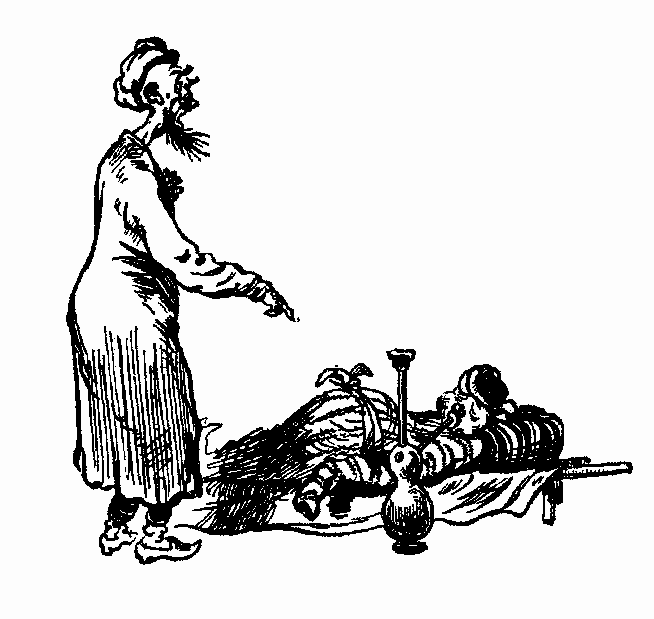
\includegraphics[width=\textwidth]{10.png}
\end{figure}

Ходжа Насреддин протискался в~толпу, приподнялся на~цыпочках и~увидел длинного, костлявого муллу, с~маленькими злыми глазами и~реденькой бороденкой. Он~кричал, тыча пальцем вниз, себе под ноги, где на~носилках лежал параличный:

—~Смотрите, смотрите, мусульмане, как он~жалок и~несчастен, но~через неделю святой Богаэддин пошлет ему исцеление, и~он~вернется к~жизни, этот человек!

Параличный лежал с~закрытыми глазами, сохраняя на~лице скорбное и~жалостное выражение. Ходжа Насреддин тихонько ахнул от~неожиданности: эту рябую рожу с~плоским носом он~отличил~бы из~тысячи других, сомнения быть не~могло! Слуга, по-видимому, заболел параличом уже давно, ибо от~долгого лежания и~безделья рожа его потолстела заметно.

С~тех пор, сколько~бы ни~проходил Ходжа Насреддин мимо этой мечети, всегда он~видел там муллу и~параличного, что лежал с~жалобным выражением на~рябой роже, которая толстела и~наливалась жиром день ото дня.

Наступил праздник памяти святейшего шейха. Святой умер, по~преданию, в~мае, в~ясный полдень, и~хотя на~небе не~было ни~одной тучки, но~солнце померкло в~час его смерти, земля дрогнула, и~многие дома, где жили грешники, подверглись разрушению, а~сами грешники погибли под развалинами. Так рассказывали муллы в~мечетях, призывая мусульман обязательно посетить гробницу шейха и~поклониться его праху, дабы не~прослыть нечестивцами и~не~разделить участи упомянутых грешников.

Богомольцы двинулись на~поклонение еще затемно, и~когда взошло солнце, то~вся огромная площадь вокруг гробницы была уже затоплена народом из~конца в~конец. Но~потоки людей на~дорогах не~истощались; все шли босиком, как требовал того стародавний обычай; здесь среди прочих были люди, пришедшие из~отдаленных мест,~— особо благочестивые или~же, наоборот, сотворившие большой грех и~надеявшиеся вымолить сегодня прощение. Мужья вели сюда бесплодных жен, матери несли, больных детей, старики тащились кое-как на~кривых костылях, прокаженные собрались поодаль и~оттуда с~надеждой смотрели на~белый купол гробницы.

Богослужение не~начиналось долго: ждали эмира. Под палящим солнцем, в~давке и~тесноте, люди стояли, плотно прижавшись друг к~другу и~не~осмеливаясь присесть. Глаза людей горели жадным, неутолимым огнем: разуверившись в~земном счастье, люди ждали сегодня чуда и~вздрагивали от~каждого громкого слова. Ожидание становилось непереносимым, два дервиша упали в~корчах на~землю и~с~воплями начали грызть~ее, источая серую пену. Толпа всколыхнулась, заволновалась, во~всех концах заплакали, закричали женщины, и~в~это время прокатился тысячеголосый рокот:

—~Эмир! Эмир!

Дворцовая стража, усердно работая палками, расчищала дорогу в~толпе, и~по~этой широкой дороге, застланной коврами, шел на~поклонение святому праху эмир~— босой, с~опущенной головой, погруженный в~благочестивые размышления и~недоступный мирским звукам. За~ним по~пятам следовала в~молчании свита, суетились слуги, свертывая ковры и~занося их~вперед.

В~толпе у~многих выступили на~глазах слезы умиления.

Эмир поднялся на~земляное возвышение, примыкавшее вплотную к~стене гробницы. Ему подали молитвенный коврик, и~он, поддерживаемый с~обеих сторон визирями, стал на~колени. Муллы в~белых одеждах выстроились полукругом и~запели, воздевая руки к~замутившемуся от~зноя небу. Богослужение началось.

Оно продолжалось бесконечно, перемежаемое проповедями. Ходжа Насреддин незаметно выбрался из~толпы и~направился к~стоявшему в~стороне небольшому сарайчику, где ждали своей очереди слепые, хромые и~параличные, которым сегодня было обещано исцеление.

Двери сарайчика были раскрыты настежь. Любопытные заглядывали внутрь и~обменивались замечаниями. Муллы, наблюдавшие здесь, держали на~руках большие медные подносы для сбора пожертвований. Старший мулла рассказывал:

—~...и с~тех пор над священной Бухарой и~над ее~солнцеподобными эмирами вечно и~нерушимо пребывает благословение святейшего шейха Богаэддина. И~каждый год в~этот день святой Богаэддин дает нам, смиренным служителям бога, силу творить чудеса. Все эти слепые, хромые, бесноватые в~параличные ждут исцеления, и~мы~надеемся с~помощью святого Богаэддина сегодня избавить их~от~страданий.

Словно~бы в~ответ ему, в~сарайчике заплакал завыли, застонали и~заскрежетали зубами; возбысив голос, мулла продолжал:

—~Жертвуйте, правоверные, на~украшение мечетей, и~ваши даяния зачтутся аллахом!

Ходжа Насреддин заглянул в~сарайчик. У~самого выхода лежал на~своих носилках рябой, толстомордый слуга; за~ним в~полумраке виднелось еще множество людей с~костылями, на~носилках, в~повязках. И~вдруг от~гробницы долетел голос самого главного ишана\footnote{Ишан~— глава мусульманской общины, обычно принадлежавший к~одному из~орденов дервишей и~подобным им~группам населения.} только что закончившего проповедь:

—~Слепого! Подведите ко~мне слепого! Муллы, оттолкнув Ходжу Насреддина, нырнули в~душный полусумрак сарайчика и~через минуту вывели оттуда слепого в~жалком нищенском рубище. Он~шел, ощупывая руками воздух и~спотыкаясь о~камни.

Он~подошел к~главному ишану, упал перед ним и~коснулся губами ступеней гробницы; ишан возложил руки на~его голову~— и~он~исцелился мгновенно.

—~Я~вижу! Вижу! —~закричал он~высоким, дрожащим голосом. —~О~святейший Богаэддин, я~вижу, я~вижу! О~небывалое исцеление, о~великое чудо!

Толпа молящихся сгрудилась вокруг него, загудела; многие подходили к~нему и~спрашивали: «Скажи, какую руку я~поднял~— правую или левую?»~— он~отвечал без ошибки, и~все удостоверились, что действительно он~прозрел.

И~тогда в~толпу двинулся целый отряд мулл с~медными подносами, взывая:

—~Правоверные, вы~своими глазами видели чудо; пожертвуйте на~украшение мечетей!

Эмир первый бросил на~поднос горсть золотых монет, за~ним бросили по~золотой монете все визири и~сановники, а~потом народ начал щедро сыпать серебро и~медь; подносы наполнялись, и~муллам трижды пришлось менять~их.

Когда поток пожертвований уменьшился, из~сарайчика вывели хромого, и~он, коснувшись ступеней гробницы, исцелился также мгновенно~и, отшвырнув свои костыли, начал плясать, высоко подбрасывая ноги. И~опять муллы с~новыми подносами двинулись в~толпу, взывая:

—~Пожертвуйте, правоверные!

Седобородый, мулла подошел к~Ходже Насреддину, который сосредоточенно думал о~чем-то, разглядывая стены сарайчика.

—~О~правоверный? Ты~видел великое чудо. Пожертвуй" и~даяние твое зачтется аллахам.

Ходжа Насреддин громко, чтобы слышали все окружающие, ответил:

—~Ты~называешь это чудом и~просишь у~меня денег. Во-первых, денег у~меня нет, а~во-вторых, известно~ли тебе, мулла, что я~сам~— великий святой и~могу сотворить еще не~такое чудо!

—~Ты~богохульник! —~закричал мулла в~гневе. —~Не~слушайте его, мусульмане, это сам шайтан говорит его устами!

Ходжа Насреддин обратился к~толпе:

—~Мулла не~верит, что я~могу творить чудеса! Хорошо, я~сейчас докажу! В~этом сарайчике собраны слепые, хромые, немощные и~параличные, и~я~берусь исцелить их~всех разом и~при этом не~буду прикасаться к~ним. Я~скажу только два слова~— и~они все исцелятся и~побегут врассыпную так быстро, что даже лучший арабский конь не~догонит~их. Стены сарайчика были тонкими, глина во~многих местах дала глубокие трещины. Ходжа Насреддин выбрал в~стене место, со~всех сторон прорезанное трещинами, сильно нажал на~него плечом. Глина подалась с~легким, зловещим треском. Он~поднажал еще, огромный кусок стены рухнул с~гулким шумом внутрь сарайчика; из~черного зияющего отверстия повалила пыль.

—~Землетрясение! Спасайтесь! —~диким голосом вскрикнул Ходжа Насреддин и~обрушил второй кусок глины.

В~сарайчике на~одно мгновение стало тихо, потом поднялась суматоха: рябой параличный слуга первым бросился к~выходу, но~застрял в~дверях со~своими носилками и~загородил путь остальным~— хромым, слепым и~немощным, которые клубились сзади с~криками и~воем, а~когда Ходжа Насреддин обрушил в~сарайчик третий пласт глины~— они могучим напором вынесли рябого вместе с~дверью и~косяками~и, позабыв про свои увечья, кинулись кто куда.

Толпа кричала, свистела, хохотала и~улюлюкала. Перекрывая общий гул, звучал громкий голос Ходжи Насреддина:

—~Вот видите, мусульмане, я~был прав, говоря, что их~всех можно исцелить одним словом!

И, не~внимая больше проповедям, со~всех сторон бежали любопытные~и, узнав, валились от~смеха на~землю, передавали дальше рассказ о~чудесном исцелении; тотчас~же об~этом узнали все собравшиеся, и~когда главный ишан поднял руку, призывая к~тишине, толпа ответила руганью, криком и~свистом.

И~опять, как тогда на~площади, в~толпе нарастало, и~гудело, и~отдавалось:

—~Ходжа Насреддин! Он~вернулся! Он~здесь, наш Ходжа Насреддин!

Муллы, осыпаемые бранью и~насмешками, побросали свои подносы и~в~страхе убежали из~толпы.

Ходжа Насреддин был в~это время уже далеко. Свою цветную чалму и~фальшивую бороду он~спрятал под халат, ибо сейчас не~имел причин опасаться встречи со~шпионами, которым было достаточно дела вокруг гробницы.

Он~не~заметил только, что за~ним по~пятам, скрываясь за~углами домов и~придорожными деревьями, следовал хромой ростовщик Джафар.

В~безлюдном, пустынном переулке Ходжа Насреддин подошел к~забору~и, подтянувшись на~руках, тихонько кашлянул. Послышались легкие шаги, женский голос ответил:

—~Это~ты, мой любимый!

Притаившийся за~деревом ростовщик без труда узнал голос прекрасной Гюльджан. Потом он~услышал шепот, сдержанный смех и~звуки поцелуев. «Ты~отнял ее~у~меня, чтобы воспользоваться самому»,~— думал ростовщик, обуреваемый злобной ревностью.

Простившись с~Гюльджан, Ходжа Насреддин пошел дальше так быстро, что ростовщик уже не~мог успеть за~ним и~скоро потерял его в~путанице узких переходов. «Значит, я~не~получу награды за~его поимку,~— думал Джафар с~огорчением. —~Но~зато!.. Берегись, Ходжа Насреддин, я~приготовил тебе страшную месть!»


\chapter{}

Эмирская казна понесла большие убытки. У~гробницы святого Богаэддина не~собрали и~десятой части по~сравнению с~доходами прошлых лет. Кроме того, в~народ были снова брошены семена дерзкого вольнодумия. Шпионы доносили, что слух о~событиях вокруг гробницы достиг самых отдаленных уголков государства и~пробудил уже отклики: в~трех кишлаках жители отказались достраивать мечети, а~в~четвертом~— выгнали с~позором своего муллу.

Эмир приказал великому визирю Бахтияру собрать диван~— государственный совет. Диван собрался в~дворцовом саду. Это был замечательный сад, один из~прекраснейших в~мире. Диковинные плоды зрели здесь на~раскидистых, пышных деревьях~— абрикосы камфарные, миндальные и~хорасанские, сливы, инжир, померанцы и~много других плодов, перечислить которые невозможно. Розы, фиалки, левкои и~лаванда с~анемонами росли целыми купами, наполняя воздух райским благоуханием; смеялись ромашки, и~влюбленно смотрели на~них нарциссы; плескались фонтаны, золотые рыбки стаями гуляли в~мраморных бассейнах, и~повсюду были развешаны серебряные клетки, в~которых звенели, свистели и~щебетали на~разные голоса чужеземные птицы. Но~визири, сановники, мудрецы и~поэты равнодушно проходили мимо, не~пленяясь волшебной красотой, ничего не~видя и~не~слыша, ибо все мысли их~были заняты заботами о~собственном возвышении, о~предохранении себя от~ударов со~стороны врагов и~о~нанесении в~свою очередь таких~же ударов, и~в~их~жестких, высохших сердцах не~оставалось уже места ни~для чего другого, и~если~бы вдруг все цветы во~всем мире завяли и~все птицы на~свете перестали петь~— они~бы не~заметили этого, поглощенные своими честолюбивыми и~алчными помыслами. С~глазами, лишенными блеска, с~поджатыми бескровными губами, они шли, шаркая туфлями, по~песчаным дорожкам, поднимались в~беседку, оплетенную пышной и~темной листвой базилика, и, прислонив к~стене свои посохи, разукрашенные бирюзой, занимали места на~шелковых подушках. Склонив головы, отягощенные огромными белыми чалмами, они в~безмолвии ждали повелителя. Когда он~вошел~— тяжелым шагом, ни~на~кого не~глядя, с~печатью мрачной задумчивости на~лице,~— все встали; склонились в~поклонах почти до~земли и~так, не~разгибаясь, стояли, пока он~не~подал им~рукой короткого знака. Тогда они стали на~колени, как этого требовал придворный обычай, и~откинулись всем телом на~пятки, касаясь при этом ковра пальцами опущенных рук; каждый из~них старался угадать, на~чью голову обрушится сегодня гнев эмира и~какую пользу можно будет извлечь из~этого для себя.

За~спиной эмира выстроились полукругом в~обычном порядке придворные поэты и~тихонько покашливали, прочищая гортани. Самый искусный из~них, носивший титул царя поэтов, повторял в~памяти сочиненные сегодня утром стихи, готовясь произнести их~перед эмиром, как~бы в~порыве сверхъестественного вдохновения.

Дворцовый мухобой и~эмирский кальянщик заняли назначенные места.

—~Кто повелитель Бухары? —~начал эмир тихим голосом, заставившим всех содрогнуться. —~Кто повелитель Бухары, мы~вас спрашиваем, мы~или он~— этот проклятый богохульник Ходжа Насреддин?!

Он~задохнулся на~мгновение; справившись со~своей яростью, грозно закончил:

—~Эмир слушает вас! Говорите.

Над его головой качались опахала из~конских хвостов; свита молчала, объятая страхом, визири незаметно подталкивали друг друга локтями.

—~Он~взбаламутил все государство! —~снова начал эмир. —~Он~уже трижды успел возмутить спокойствие в~нашей столице! Он~лишил нас покоя и~сна, а~нашу казну лишил законных доходов! Он~открыто призывает народ к~возмущению и~бунту! Как следует поступить с~таким преступником? —~мы~вас спрашиваем.

Визири, сановники и~мудрецы ответили в~один голос:

—~Он~бесспорно заслуживает самой жестокой казни, о~средоточие вселенной и~убежище мира!

—~Почему~же он~до~сих пор еще жив? —~спросил эмир. —~Или нам, вашему повелителю, самое имя которого должны вы~произносить с~трепетом и~благоговением и~не~иначе, как лежа ниц на~земле, чего~вы, кстати, не~делаете по~своей лености, дерзости и~нерадивости,~— или, повторяю, нам самому нужно идти на~базар и~ловить его, в~то~время как вы~будете предаваться праздному чревоугодию и~разврату в~своих гаремах и~вспоминать о~своих обязанностях перед нами только в~дни получения жалованья? Что ты~ответишь нам, Бахтияр?

Услышав имя Бахтияра, все остальные облегченно вздохнули. По~губам Арсланбека, у~которого была с~Бахтияром старинная вражда, скользнула злорадная усмешка. Бахтияр, сложив на~животе руки, поклонился эмиру до~земли.

—~Да~хранит аллах великого эмира от~бед и~несчастий! —~начал~он. —~Преданность и~заслуги ничтожного раба, который является лишь пылинкой в~лучах величия эмира, известны эмиру. До~моего назначения на~должность великого визиря государственная казна пребывала всегда пустою. Но~я~назначил множество пошлин, установил плату за~назначение и~должность, я~обложил налогами все в~Бухаре, и~ныне ни~один житель не~может даже чихнуть, без того чтобы не~уплатить за~это в~казну. Кроме того, я~наполовину уменьшил жалованье всем мелким чиновникам, солдатам и~стражникам, возложив заботы о~пропитании их~на~жителей Бухары, чем сберег эмир-ской казне, о~повелитель, немалую толику. Но~я~еще не~все сказал о~моих заслугах: своими стараниями я~достиг того, что у~гробницы святейшего шейха Богаэддина вновь начали совершаться чудеса, что привлекло к~этой гробнице многие тысячи паломников, и~казна владыки нашего, перед которым все остальные государи мира не~что иное, как прах, каждый год переполнялась пожертвованиями, и~доходы умножились многократно...

—~Где они, эти доходы? —~перебил эмир. —~Их~отнял у~нас Ходжа Насреддин. И~мы~спрашиваем тебя не~о~твоих заслугах~— об~этом мы~слышали уже много раз. Ты~лучше скажи: как поймать Ходжу Насреддина?

—~О~повелитель! —~ответил Бахтияр. —~В~обязанности великого визиря не~входит поимка преступников. Такие дела в~нашем государстве поручены почтенному Арсланбеку, начальнику дворцовой стражи и~войска.

С~этими словами он~еще раз до~земли поклонился эмиру, посмотрев с~торжеством и~злорадством на~Арсланбека.

—~Говори! —~приказал эмир.

Арсланбек встал, метнул на~Бахтияра злобный взгляд. Он~глубоко вздохнул, его черная борода всколыхнулась на~брюхе.

—~Да~хранит аллах нашего солнцеподобного владыку от~бед и~несчастий, от~болезней и~огорчений! Мои заслуги известны эмиру. Когда хивинский хан пошел войной на~Бухару, то~эмиру, средоточию вселенной и~тени аллаха на~земле, благоугодно было поручить мне главенство над бухарским войском. И~я~распорядился так, что мы~без кровопролития победоносно отразили врага и~все дело окончилось к~нашему благу. А~именно: от~самой границы хивинской и~вглубь нашей страны на~многие дни перехода все города и~селения были, по~моему приказанию, превращены в~развалины, посевы и~сады истреблены, дороги и~мосты разрушены. И~когда хивинцы вступили на~нашу землю и~увидели одну пустыню без садов и~без жизни, они сказали себе: «Не~пойдем в~Бухару, ибо там нечего есть и~нечем поживиться». Они повернули обратно и~ушли, осмеянные и~поруганные! И~наш владыка эмир признать тогда соизволил, что разорение страны своим~же войском есть дело столь мудрое и~полезное, что распорядился ничего не~исправлять и~оставить города, селения, поля и~дороги в~том~же разрушенном виде, дабы и~впредь чужеземные племена не~дерзали вступать на~нашу землю. Так я~победил хивинцев. Кроме того, я~завел в~Бухаре многие тысячи шпионов...

—~Замолчи, хвастун! —~воскликнул эмир. —~Почему~же твои шпионы до~сих пор не~поймали Ходжу Насреддина?

Арсланбек долго молчал в~замешательстве, наконец признался:

—~О~повелитель, я~применял всякие способы, но~мой разум бессилен против этого злодея и~богохульника. Я~думаю, повелитель, что следует спросить совета у~мудрецов.

—~Клянемся нашими предками, вы~все достойны того, чтобы повесить вас на~городской стене! —~вспылил эмир и~в~раздражении отвесил мимоходом затрещину своему кальянщику, который как раз подсунулся в~это время под его царственную длань. —~Говори! —~приказал он~самому старому мудрецу, славившемуся среди прочих своей бородой, которой он~мог дважды обвязаться, как поясом.

Мудрый встал~и, сотворив молитву, огладил свою знаменитую бороду, что удалось ему сделать не~сразу, а~лишь постепенно, продергивая ее~правой рукой сквозь пальцы левой руки.

—~Да~продлит бесконечно аллах сверкающие дни повелителя на~благо и~радость народу! —~начал~он. —~Так как вышеназванный злодей и~возмутитель Ходжа Насреддин является все~же человеком, то~можно заключить, что тело его устроено так~же, как и~у~всех остальных людей, то~есть состоит из~двухсот сорока костей и~трехсот шестидесяти жил, управляющих легкими, печенью, сердцем, селезенкой и~желчью. Основой всех жил является, как этому учат нас мудрые, сердечная жила, от~которой расходятся все остальные, и~это есть непреложная и~святая истина, в~противоположность еретическому учению нечестивого Абу-Исхака, осмеливающегося ложно утверждать, будто~бы основой жизни человека является жила легочная. В~соответствии с~книгами мудрейшего Авиценны, благочестивейшего Мухаммед-аль-Расуля, греческого лекаря Гиппократа, а~также Аверроэса из~Кордовы, плодами размышлений которых питаемся мы~до~сих пор, а~также в~соответствии с~учениями аль-Кенди, аль-Фараби и~Абубацера-ибн-Туфейля, скажу и~осмелюсь утверждать, что аллах создал Адама сложенным из~четырех стихий~— воды, земли, огня и~воздуха, и~сделал при этом так, чтобы у~желтой желчи была природа огня, что мы~и~видим в~действительности, ибо она~— горячая и~сухая, у~черной желчи~— природа земли, ибо она~— холодная и~сухая, у~слюны~— природа воды, ибо она~— холодная и~влажная, у~крови~— природа воздуха, ибо она~— горячая и~влажная. И~если лишить человека какой-либо одной из~этих заключающихся в~нем жидкостей, то~означенный человек неминуемо умрет, исходя из~чего, я~и~полагаю, о~пресветлый повелитель, что следует лишить означенного богохульника и~возмутителя Ходжу Насреддина крови, что предпочтительнее всего сделать через отделение его головы от~его туловища, ибо вместе с~вытекающей кровью из~тела человека улетучивается жизнь и~не~возвращается более. Вот мой совет, о~пресветлый владыка и~убежище мира!

Эмир выслушал все это со~вниманием~и, ничего не~ответив, едва заметным движением бровей подал знак второму мудрецу, который хотя и~уступал первому в~длине своей бороды, но~зато неизмеримо превосходил его размерами и~пышностью чалмы, непомерная тяжесть коей искривила за~многие годы вбок и~вниз его шею, что придавало ему вид человека, вечно подглядывающего снизу вверх сквозь узкую щелку. Поклонившись эмиру, он~сказал:

—~О~великий владыка, подобный солнцу блеском своим! Я~не~могу согласиться с~этим способом избавления от~Ходжи Насреддина, ибо известно, что не~только кровь необходима для жизни человека, но~также и~воздух, и~если сдавить человеку горло веревкой и~прекратить тем самым доступ воздуха в~его легкие, то~человек неминуемо умирает и~не~может уже воскреснуть потом...

—~Так! —~сказал эмир тихим голосом. —~Вы~совершенно правы, о~мудрейшие из~мудрых, и~советы ваши, без сомнения, драгоценны для нас! Ну, как~бы, действительно, избавились мы~от~Ходжи Насреддина, если~бы вы~не~дали нам таких драгоценных советов!

Он~остановился, не~в~силах совладать с~охватившими его гневом и~яростью; щеки его дрожали, ноздри раздувались, в~глазах полыхали молнии. Но~придворные льстецы~— философы и~стихотворцы, что стояли, выстроившись полукругом за~эмирской спиной,~— не~видели грозного лица своего владыки и~потому не~уловили гнева и~насмешки в~его словах, обращенных к~мудрецам, и, приняв эти слова за~чистую монету, решили, что мудрецы действительно отличились перед эмиром, будут приближены к~нему и~осыпаны его милостями, почему и~следует немедленно заручиться их~благорасположением, дабы в~дальнейшем извлечь из~этого для себя пользу.

—~О~мудрейшие, о~жемчужины, украшающие венец нашего пресветлого владыки, о~мудрые, превзошедшие своей мудростью самую мудрость и~умудренные мудростью наимудрейших!

Так они славословили, стараясь превзойти друг друга изысканностью и~усердием и~не~замечая, что эмир, повернувшись, смотрит на~них, содрогаясь от~ярости, пронзительным взглядом, а~вокруг воцарилась зловещая тишина.

—~О~светочи знаний и~сосуды разума! —~продолжали они, закрыв в~самозабвении глаза и~трепеща от~сладостного раболепия. Но~вдруг царь поэтов заметил взгляд эмира и~сразу точно~бы проглотил свой льстивый язык~— и~попятился, охваченный ужасом, а~вслед за~ним умолкли все остальные и~задрожали, поняв свой промах, проистекший от~чрезмерного желания восхвалить.

—~О~бездельники, о~мошенники! —~воскликнул эмир с~негодованием. —~Как будто мы~с~вами не~знаем, что если отрубить человеку голову или удавить его веревкой, то~он~уже не~воскреснет больше! Но~для этого нужно сначала поймать человека, вы~же, бездельники, ленивцы, мошенники и~глупцы, не~сказали ни~слова о~том, как его поймать. Всех визирей, сановников, мудрецов и~стихотворцев, присутствующих здесь, мы~лишаем жалованья до~тех пор, пока не~будет пойман Ходжа Насреддин. И~приказываем объявить награду поймавшему его в~три тысячи таньга! И~еще предупреждаем, что, убедившись в~вашей лености, тупости и~нерадивости, мы~выписали из~Багдада к~себе на~службу нового мудреца, по~имени Гуссейн Гуслия, служившего до~сих пор у~моего друга калифа багдадского. Он~находится уже в~пути, скоро прибудет, и~тогда горе вам, о~уминатели тюфяков, поглотители пищи и~набиватели своих бездонных карманов! продолжал~он, распаляясь все больше и~больше. —~Гнать их! —~закричал он~стражникам. —~Гнать их~всех отсюда! Гнать в~шею!

Стражники бросились к~оцепеневшим придворным, хватали их~без всякого разбора и~почтения, тащили к~двери и~свергали оттуда вниз помимо лестницы, а~внизу подхватывали их~другие стражники, провожали подзатыльниками, затрещинами, тычками и~пинками; придворные бежали, перегоняя друг друга; седой мудрец упал, запутавшись в~своей бороде, а~споткнувшись о~него, рухнул и~второй мудрец~— головой прямо в~колючий розовый куст~и, ошеломленный падением, долго лежал там со~своей искривленной шеей, словно~бы подглядывая снизу вверх сквозь узкую щелку.


\chapter{}

Эмир был мрачен и~грозен до~самого вечера. Прошла ночь, а~утром объятые страхом придворные снова узрели темную печать гнева на~его лице.

Тщетны были все усилия развлечь и~развеселить его, тщетно в~дыму благовонных курений изгибались перед ним танцовщицы с~бубнами в~руках, раскачивали полные бедра, блестели жемчугами зубов, обнажали, словно~бы невзначай, свои смуглые груди,~— он~не~поднимал тяжелого взора, и~судорога пробегала по~его лицу, приводя в~трепет сердца придворных. Напрасны были все ухищрения шутов, акробатов, фокусников и~индийских факиров, усыпляющих змей пением тростниковых свирелей.

Придворные перешептывались между собой:

—~О~проклятый Ходжа Насреддин, о~сын греха! Сколько неприятностей мы~терпим из-за него! Все с~надеждой обращали взоры к~Арсланбеку. Он~собрал в~караульном помещении наиболее искусных шпионов, среди которых был и~рябой шпион, так чудесно исцеленный Ходжой Насреддином от~паралича.

—~Знайте~же,~— говорил Арсланбек,~— что вы~по~приказанию нашего светлейшего эмира лишаетесь жалованья до~тех пор, пока не~будет пойман злодей Ходжа Насреддин! А~если вы~не~выследите его, то~лишитесь не~только жалованья, но~и~голов, что я~вам обещаю твердо. И, напротив того, приложивший все усердие и~поймавший Ходжу Насреддина получит награду в~три тысячи таньга, а~сверх того получит еще повышение по~службе: он~будет назначен главным шпионом.

Шпионы немедля отправились на~работу, переодетые дервишами, нищими, водоносами и~торговцами, а~рябой шпион, превосходивший остальных своею хитростью, взял коврик, бобы, четки, старинные книги и~пошел на~базар, на~перекресток между ювелирным и~мускусным рядами, где намеревался, изображая гадальщика, расспросить хорошенько женщин.

А~часом позже на~базарную площадь вышли сотни глашатаев, призывавших своими криками всех мусульман ко~вниманию. Они возгласили эмирский фирман\footnote{Фирман~— так именовался указ, который издавался правителем в~некоторых мусульманских странах.}. Ходжа Насреддин объявлялся врагом эмира и~осквернителем веры, жителям воспрещались всякие сношения с~ним, а~наипаче~— укрывательство его, за~что виновные будут подвергаться немедленной смерти. Тому~же, кто предаст его в~руки эмирской стражи, обещалась награда в~три тысячи таньга и~прочие милости.

Чайханщики, медники, кузнецы, ткачи, водоносы, погонщики перешептывались:

—~Ну, эмиру придется ждать долго!

—~Не~таков наш Ходжа Насреддин, чтобы попасться!

—~И~не~таковы жители Благородной Бухары, чтобы польститься на~деньги и~предать своего Ходжу Насреддина!

Но~ростовщик Джафар, совершавший сегодня обычный поход по~базару и~терзавший своих должников, думал иначе. «Три тысячи таньга! —~сокрушался~он. —~Вчера эти деньги были у~меня почти что в~кармане! Ходжа Насреддин опять придет к~этой девушке, но~я~в~одиночку не~сумею поймать его, если~же я~скажу кому-нибудь, то~у~меня отобьют награду! Нет, я~поступлю иначе!»

Он~отправился во~дворец.

Долго стучал~он. Ему не~открывали. Стражники не~слышали: они оживленно беседовали, придумывая планы поимки Ходжи Насреддина.

—~О~доблестные воины, вы~что, заснули там? —~взывал отчаянным голосом ростовщик, гремя железным кольцом, но~прошло много времени, прежде чем раздались шаги, лязг засовов~— и~калитка открылась.

Арсланбек, выслушав ростовщика, покачал головой:

—~Почтенный Джафар, я~не~советую тебе ходить сегодня к~эмиру. Он~грозен и~мрачен.

—~У~меня как раз есть отличное средство развеселить его,~— возразил ростовщик. —~О~почтенный Арсланбек, оплот трона и~усмиритель врагов, дело мое не~терпит отлагательства. Пойди скажи эмиру, что я~пришел развеять его печаль.

Эмир встретил ростовщика сумрачно:

—~Говори, Джафар. Но~если твоя новость не~развеселит нас, ты~получишь тут~же на~месте две сотни палок.

—~О~великий владыка, затмевающий блеском своим всех царей, предшествовавших, настоящих и~будущих,~— сказал ростовщик,~— мне, ничтожному, известно, что в~нашем городе живет одна девушка, которую смело назову перед лицом истины прекраснейшей из~всех прекрасных.

Эмир оживился, поднял голову.

—~О~повелитель! —~продолжал осмелевший ростовщик. —~У~меня нет слов, чтобы достойно восхвалить ее~красоту. Она~— высокая ростом, прелестная, стройная и~соразмерная, с~сияющим лбом и~румяным лицом, с~глазами, напоминающими глаза газели, с~бровями, подобными тонкому месяцу! Ее~щеки~— как анемоны, и~рот~— как сулейманова печать, и~губы ее~— как коралл, и~зубы~— как жемчуг, и~грудь~— как мрамор, украшенный двумя вишнями, и~плечи...

Эмир остановил поток его красноречия:

—~Если девушка действительно такова, как ты~говоришь, то~она достойна занять место в~нашем гареме. Кто она?

—~Девушка простого и~незнатного рода, о~повелитель. Это~— дочь одного горшечника, ничтожным именем которого я~не~осмелюсь оскорбить слух повелителя. Я~могу указать ее~дом, но~будет~ли за~это награда преданному рабу эмира?

Эмир кивнул Бахтияру: к~ногам ростовщика упал кошелек. Ростовщик схватил его, переменившись в~лице от~алчности.

—~Если она окажется достойной твоих восхвалений, ты~получишь еще столько~же,~— сказал эмир.

—~Слава щедрости нашего владыки! —~воскликнул ростовщик. —~Но~пусть повелитель спешит, ибо мне известно, что за~этой серной охотятся!

Брови эмира сошлись, глубокая морщина рассекла переносицу:

—~Кто?

—~Ходжа Насреддин! —~ответил ростовщик.

—~Опять Ходжа Насреддин! И~здесь Ходжа Насреддин! Он~успевает всюду, этот Ходжа Насреддин, а~вы,~— и, покачнув трон, эмир резко повернулся к~визирям,~— вы~всегда опаздываете, ничего не~делаете и~подвергаете посрамлению наше величие. Эй, Арсланбек! Чтоб эта девушка была немедленно доставлена сюда, во~дворец, а~если ты~не~приведешь~ее, тебя встретит на~обратном пути палач!

Не~прошло и~пяти минут, как из~ворот дворца вышел, звеня оружием и~сверкая на~солнце щитами, большой отряд стражников под командой самого Арсланбека, прицепившего к~парчовому халату золоченую бляху в~знак своей силы и~власти.

Сбоку, прихрамывая и~гнусно ковыляя, шел ростовщик; он~поминутно отставал от~стражников и~нагонял их~вприпрыжку. Народ сторонился, провожал ростовщика недобрыми взглядами, пытаясь угадать, какое новое злодейство он~затеял.


\chapter{}

Ходжа Насреддин только что закончил девятый по~счету горшок~и, поставив его на~солнце, взял из~корыта большой ком глины для следующего, десятого горшка.

В~калитку вдруг постучали~— властно и~громко. Соседи, часто забегавшие к~Ниязу, чтобы занять луковицу или щепотку перца, стучали не~так. Ходжа Насреддин и~Нияз переглянулись тревожно, а~калитка опять загудела под градом тяжелых ударов. На~этот раз Ходжа Насреддин ухом уловил звон железа и~меди. «Стража»,~— шепнул он~Ниязу. «Беги»,~— ответил Нияз. Ходжа Насреддин махнул через забор, а~Нияз долго еще возился у~калитки, чтобы дать ему время уйти подальше. Наконец~— откинул щеколду. В~тот~же миг из~виноградника брызнули во~все стороны скворцы. Но~у~старого Нияза не~было крыльев, он~не~мог улететь. Он~побледнел, задрожал, согнулся в~поклоне перед Арсланбеком.

\begin{figure}[h]
\centering
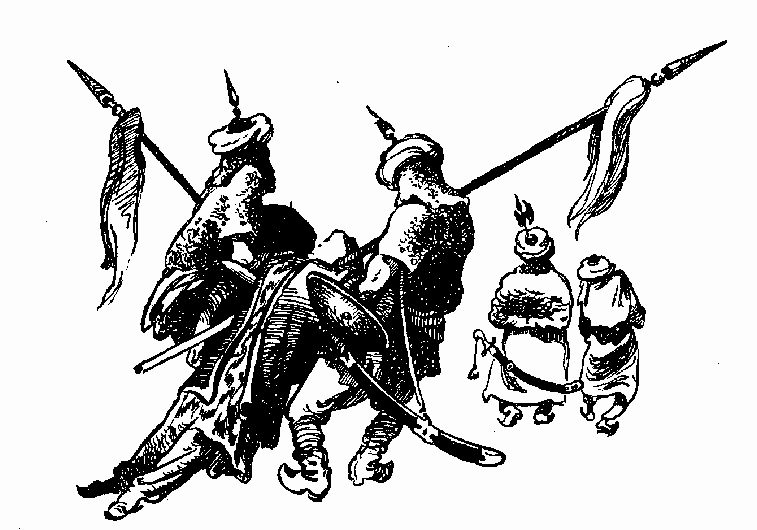
\includegraphics[width=\textwidth]{11.png}
\end{figure}

—~Твоему дому, горшечник, выпала великая честь,~— сказал Арсланбек. —~Повелитель правоверных и~наместник аллаха на~земле, наш господин и~владыка, да~продлятся его благословенные годы, сам великий эмир соизволил вспомнить твое ничтожное имя! До~него дошло, что в~твоем саду растет прекрасная роза, и~он~пожелал украсить этой розой свой дворец. Где твоя дочь?

Седая голова горшечника затряслась, свет померк перед его глазами. Глухо услышал он~короткий, словно~бы предсмертный, стон своей дочери, которую стражники вытащили из~дома во~двор. Ноги старика подломились в~коленях, он~упал на~землю вниз лицом и~больше не~видел и~не~слышал уже ничего.

—~Он~лишился чувств от~столь великого счастья,~— пояснил Арсланбек своим стражникам. —~Не~трогайте его, пусть он~очнется, а~потом пусть придет во~дворец, чтобы излить перед эмиром свою безграничную благодарность. Идемте.

Ходжа Насреддин в~это время успел обежать кругом и~вышел на~ту~же улицу с~другой стороны. Он~притаился за~кустами. Отсюда он~видел калитку дома Нияза, двух стражников у~калитки и~третьего человека, в~котором, присмотревшись, узнал ростовщика Джафара. «Ага, хромая собака! Это, значит, ты~привел сюда стражников, чтобы схватить меня! —~думал~он, все еще не~догадываясь об~истине. —~Ну, ладно, ищите! Придется вам уйти с~пустыми руками!»

Нет! Они ушли не~с~пустыми руками! Похолодевший от~ужаса Ходжа Насреддин видел, как вывели они из~калитки его возлюбленную. Она пыталась вырваться, кричала надломленным голосом, стражники держали ее~крепко, огородив двойным кольцом щитов.

Был июньский полдень~— очень жарко, но~Ходжу Насреддина бил озноб, а~стражники приближались; дорога шла мимо тех кустов, за~которыми притаился Ходжа Насреддин. Рассудок его помутился. Он~вытащил из~ножен кривой нож и~припал к~земле. Ареланбек шел впереди, сияя своей позолоченной бляхой, и~ему первому вонзился~бы в~жирное горло, под бороду, этот нож. Но~вдруг чья-то тяжелая рука легла на~плечо Ходжи Насреддина, сильно придавила его к~земле. Он~вздрогнул, отпрянув, занес руку с~ножом~— и~опустил~ее, увидев знакомое закопченное лицо куэнеца Юсупа.

—~Лежи! —~прошептал кузнец. —~Лежи и~не~шевелись. Ты~безумен: их~двадцать человек, и~все вооруженные, а~ты~один, и~у~тебя нет оружия, ты~погибнешь сам и~не~спасешь~ее; лежи, говорю я~тебе!

Он~держал Ходжу Насреддина прижатым к~земле до~тех пор, пока отряд стражников, сопровождавших Гюльджан, не~скрылся за~поворотом дороги.

—~Зачем, зачем удержал ты~меня! —~воскликнул Ходжа Насреддин. —~Разве не~лучше было~бы мне лежать сейчас мертвым?!

—~Рука против льва и~кулак против меча~— не~дело разумных,~— сурово ответил кузнец. —~Я~следил за~этими стражниками от~самого базара и~успел вовремя, чтобы предотвратить твой безрассудный поступок. Не~умереть должен ты~ради нее, а~бороться и~спасти~ее, что достойнее, хотя много труднее. И~не~теряй времени на~горестные размышления, иди и~действуй. У~них сабли, щиты и~копья, но~тебя аллах снабдил могучим оружием~— острым умом и~хитростью, в~которых с~тобою не~может сравниться никто.

Так он~говорил; слова его были мужественны и~тверды, как то~железо, которое ковал он~всю свою жизнь. Дрогнувшее сердце Ходжи Насреддина укрепилось, подобно железу, от~этих слов.

—~Спасибо тебе, кузнец! —~сказал~он. —~Я~не~переживал еще минут тяжелее этих, но~недостойно мне впадать в~отчаяние. Я~ухожу, кузнец, и~обещаю тебе, что своим оружием я~буду действовать доблестно!

Он~шагнул из~кустов на~дорогу. В~то~же время на~дорогу вышел из~ближайшего дома ростовщик, который задержался, чтобы напомнить одному из~гончаров о~сроке уплаты.

Они столкнулись нос к~носу. Ростовщик, побледнев, сейчас~же юркнул обратно, захлопнул дверь и~заложил ее~засовом.

—~Джафар, горе тебе, о~порождение ехидны! —~сказал Ходжа Насреддин. —~Я~все видел, все слышал, все знаю!

Была минута молчания, потом голос ростовщика ответил:

—~Вишня не~досталась шакалу. Но~она не~досталась и~соколу. Вишней завладел лев!

—~Посмотрим еще! —~сказал Ходжа Насреддин. —~А~ты, Джафар, запомни мои слова: я~вытащил тебя из~воды, но, клянусь, ты~будешь утоплен мною в~том~же самом пруду, тина облепит твое гнусное тело, водоросли задушат тебя!

Не~дожидаясь ответа, он~пошел дальше. Он~миновал дом Нияза, опасаясь, как~бы ростовщик не~подглядел и~не~донес потом на~старика; обогнув улицу и~убедившись, что никто не~следит. Ходжа Насреддин быстро пробежал заросший бурьяном пустырь и~вернулся в~дом Нияза через забор.

Старик лежал ничком на~земле. Рядом тускло поблескивала кучка серебряных денег, оставленных Арсланбеком. Старик поднял навстречу Ходже Насреддину лицо, залитое слезами, измазанное пылью; губы его искривились, он~хотел сказать что-то и~не~мог сказать, а~когда взгляд его упал на~платок, оброненный дочерью, он~начал биться седой головой о~жесткую землю и~рвать бороду.

Ходже Насреддину пришлось немало повозиться с~ним; наконец он~усадил его на~скамейку.

—~Слушай, старик! —~сказал~он. —~Ты~не~одинок в~своем горе. Знаешь~ли ты, что я~любил ее~и~она меня тоже любила? И~знаешь~ли ты, что мы~уговорились пожениться и~я~ждал только случая, когда мне удастся достать много денег и~заплатить тебе богатый выкуп?

—~Зачем мне выкуп? —~ответил старик сквозь рыдания. —~Разве я~осмелился~бы противоречить хоть в~чем-нибудь моей голубке? Но~поздно говорить об~этом, все погибло, она уже в~гареме, и~сегодня вечером эмир будет обладать~ею!.. О~горе, о~позор! —~вскричал~он. —~Я~пойду во~дворец и~упаду к~его ногам, буду умолять его, вопить и~кричать, и~если только сердце в~груди его не~каменное...

Пошатываясь, он~пошел неверными шагами к~калитке.

—~Остановись! —~сказал Ходжа Насреддин. —~Ты~забыл, что эмиры устроены совсем иначе, чем остальные люди: у~них совсем нет сердца, и~бесполезно их~умолять. У~них можно только отнять, и~я. Ходжа Насреддин,~— ты~слышишь, старик! —~отниму Гюльджан у~него!

—~Он~могуч, у~него тысячи солдат, тысячи стражников и~тысячи шпионов! Что можешь ты~сделать против него?

—~Я~не~знаю еще, что я~сделаю. Но~я~знаю только одно: он~не~войдет к~ней сегодня! И~он~не~войдет к~ней завтра. И~он~не~войдет к~ней послезавтра! И~он~никогда не~войдет к~ней и~не~будет обладать~ею, это такая~же истина, как~то, что меня зовут всюду от~Бухары до~Багдада~— Ходжа Насреддин! Уйми~же свои слезы, старик, не~вопи над самым моим ухом и~не~мешай мне думать!

Ходжа Насреддин думал недолго:

—~Старик, где у~тебя хранятся одежды твоей покойной жены?

—~Они лежат там, в~сундуке. Ходжа Насреддин взял ключ, вошел в~дом и~вскоре вышел оттуда, переодетый женщиной. Его лицо скрывала чадра, густо сплетенная из~черного конского волоса:

—~Жди меня, старик, и~сам не~предпринимай ничего.

Он~вывел из~хлева своего ишака, оседлал его и~покинул на~долгие дни дом Нияза.


\chapter{}

Перед тем как ввести Гюльджан в~дворцовый сад к~эмиру, Арсланбек вызвал из~гарема старух и~приказал им~подготовить Гюльджан, чтобы эмир-ский взор насладился созерцанием ее~совершенств. Старухи немедля взялись за~привычное дело: они вымыли теплой водой заплаканное лицо Гюльджан, переодели ее~в~легкие шелка, насурьмили ей~брови, нарумянили щеки, облили волосы розовым маслом, выкрасили ногти в~красный цвет. Затем вызвали из~гарема Его Великое Целомудрие, главного евнуха~— человека, славившегося когда-то своим распутством на~всю Бухару, призванного вследствие своих знаний и~опыта на~эмирскую службу, оскопленного придворным лекарем и~поставленного потом на~одну из~самых высших должностей в~государстве. Его обязанностью было неусыпно следить за~ста шестьюдесятью эмирскими наложницами, дабы они всегда имели соблазнительный вид и~могли пробуждать страсть в~эмире. Должность эта становилась с~каждым годом все труднее, потому что эмир пресыщался все больше, а~силы его убывали. И~главному евнуху не~раз приходилось получать утром от~своего повелителя вместо награды десяток плетей, что, впрочем, не~было для евнуха слишком мучительным наказанием, ибо~он, подготовляя прекрасных наложниц ко~встречам с~эмирам, переносил каждый раз мучения несравненно ужаснейшие и~вполне сходные с~теми, что обещаны распутникам в~аду, где упомянутые распутники осуждены находиться все время среди нагих гурий, будучи сами прикованы железными цепями к~столбам.

Когда главный евнух увидел Гюльджан, то~отступил, пораженный ее~красотой.

—~Она, поистине, прекрасна! —~воскликнул он~тонким голосом. —~Ведите ее~к~эмиру, уберите ее~прочь с~моих глаз! —~Он~пошел быстрыми шагами назад, биясь головой о~стены, громко скрежеща зубами и~восклицая: —~О, сколь мне тяжко, сколь горько!

—~Это благоприятный признак,~— сказали старухи. —~Значит, наш повелитель будет доволен.

Бедную, безмолвную Гюльджан повели во~дворцовый сад.

Эмир встал, подошел к~ней, приподнял чадру.

Все визири, сановники и~мудрецы закрыли глаза рукавами халатов.

Эмир долго не~мог оторвать взгляда от~ее~прекрасного лица.

—~Ростовщик не~солгал нам! —~сказал он~громко. —~Выдать ему награду втрое против обещанного. Гюльджан увели. Эмир заметно повеселел.

—~Он~развлекся, он~повеселел. Соловей его сердца склонился к~розам ее~лица! —~шептались придворные. —~Завтра утром он~будет еще веселее! Слава аллаху, гроза пронеслась над нами, не~поразив нас ни~громом, ни~молнией.

Придворные поэты, осмелев, выступили вперед и~поочередно начали восхвалять эмира, сравнивая в~стихах лицо его с~полной луной, стан его~— со~стройным кипарисом, а~царствование его --- с полнолунием. Царь поэтов нашел наконец случай произнести, как~бы в~порыве вдохновения, свои стихи, которые со~вчерашнего утра висели на~кончике его языка.

Эмир бросил ему горсть мелких монет. И~царь поэтов, ползая по~ковру, собирал~их, не~забыв приложиться губами к~эмирской туфле.

Милостиво засмеявшись, эмир сказал:

—~Нам тоже пришли сейчас в~голову стихи:

\begin{verse}
Когда мы~вышли вечером в~сад, \\
То~луна, устыдившись ничтожества своего, спряталась в~тучи, \\
И~птицы все замолкли, и~ветер затих, \\
А~мы~стояли~— великий, славный, непобедимый, подобный солнцу и~могучий...	
\end{verse}

Поэты все попадали на~колени, крича: «О~великий! Он~затмил самого Рудеги\footnote{Рудеги (Рудаки, около 860--941) — знаменитый поэт, родоначальник поэзии на~языке фарси.}»~— а~некоторые лежали ничком на~ковре, как~бы в~беспамятстве.

В~зал вошли танцовщицы, за~ними~— шуты, фокусники, факиры, и~всех эмир вознаградил щедро.

—~Я~жалею только,~— сказал~он,~— что не~могу повелевать солнцу, иначе я~приказал~бы ему закатиться сегодня быстрее.

Придворные отвечали подобострастным смехом.


\chapter{}

Базар гудел и~шумел, были самые горячие часы торговли, народ продавал, покупал и~обменивал, а~солнце поднималось все выше, сгоняя людей в~густую, пахучую тень крытых рядов. В~круглые окна тростниковых кровель отвесно падали яркие лучи полдня, стояли дымно-пыльными сквозными столбами, в~их~сиянии сверкала парча, блестел шелк и~мягким затаенным пламенем светился бархат; всюду мелькали, вспыхивая, чалмы, халаты, крашеные бороды; слепила глаза начищенная медь, с~нею спорило и~побеждало ее~своим чистейшим блеском благородное золото, рассыпанное перед менялами на~кожаных ковриках.

Ходжа Насреддин остановил ишака у~той самой чайханы, с~помоста которой месяц назад обратился к~жителям Бухары с~призывом спасти от~эмирской милости горшечника Нияза. Не~много времени прошло с~тех пор, но~Ходжа Насреддин успел крепко подружиться с~пузатым чайханщиком Али, человеком прямым и~честным, которому можно было довериться.

Улучив минуту. Ходжа Насреддин позвал:

—~Али!

Чайханщик оглянулся, на~лице его выразилось недоумение: голос, окликнувший его, был мужским, а~перед собой видел он~женщину.

—~Это я, Али! —~сказал Ходжа Насреддин, не~поднимая чадры. —~Ты~узнал меня? И~ради аллаха не~таращи глаза~— разве ты~забыл о~шпионах?

Али, оглянувшись, провел его в~заднюю темную комнату, где хранились дрова и~запасные чайники. Здесь было сыро, прохладно, шум базара слышался глухо.

—~Али, возьми моего ишака,~— сказал Ходжа Насреддин. —~Корми его и~держи всегда наготове! Он~может понадобиться мне в~любую минуту. И~никому ни~слова не~говори обо мне.

—~Но~почему ты~переоделся женщиной. Ходжа Насреддин? —~спросил чайханщик, прикрывая плотнее дверь. —~Куда ты~направился?

—~Я~иду во~дворец.

—~Ты~сошел с~ума! —~воскликнул чайханщик. —~Ты~хочешь сам положить голову прямо в~пасть тигру!

—~Так нужно, Али. Скоро ты~узнаешь, почему. И~давай простимся на~всякий случай,~— я~иду на~опасное дело.

Они крепко обнялись, у~доброго чайханщика выступили слезы и~покатились по~круглым красным щекам. Он~проводил Ходжу Насреддина~и, подавляя тяжелые вздохи, колыхавшие его живот, вышел к~своим гостям.

Тревога терзала сердце чайханщика, он~был грустен, рассеян, гостям приходилось дважды и~трижды звенеть крышками чайников, напоминая ему о~своей неутоленной жажде. Сердцем чайханщик был там, у~дворца, вместе со~своим неугомонным другом.

Стражники не~впустили Ходжу Насреддина.

—~Я~принесла несравненную амбру, мускус, розовое масло! —~говорил Ходжа Насреддин, искусно подделывая свой голос под женский. —~Пропустите меня в~гарем, доблестные воины, я~продам свой товар и~поделюсь прибылью с~вами.

—~Иди, иди отсюда, женщина, торгуй где-нибудь на~базаре,~— грубо отвечали стражники.

Потерпев неудачу в~своем предприятии. Ходжа Насреддин задумался и~помрачнел. Времени у~него было в~обрез, солнце перешло уже за~полуденную черту.. Ходжа Насреддин обошел вокруг дворцовой стены. Камни лежали плотно, спаянные китайским раствором, ни~одной дырки, ни~одной щели не~обнаружил в~стене Ходжа Насреддин, а~выходы арыков были забраны частыми чугунными решетками.

«Я~должен попасть во~дворец,~— сказал себе Ходжа Насреддин. —~Это мое непреклонное решение, я~его выполню! Если эмир отнял у~меня невесту по~небесному предопределению, то~почему для меня не~может быть предопределения проникнуть во~дворец и~вернуть~ее? Я~даже чувствую где-то в~глубине души, что такое предопределение есть для меня!»

Он~пошел на~базар. Он~верил, что если решение человека непреклонно и~мужество неистощимо,~— предопределение всегда придет на~помощь к~нему. Из~тысячи встреч, разговоров и~столкновений непременно будет одна такая встреча и~одно такое столкновение, которые вкупе создадут благоприятный случай, и, умело воспользовавшись~им, человек сможет опрокинуть все препятствия на~пути к~своей цели, выполнив тем самым предопределение. Где-нибудь на~базаре Ходжу Насреддина ждал такой случай. Ходжа Насреддин верил в~это непоколебимо и~отправился на~поиски его.

Ничто не~ускользало от~внимания Ходжи Насреддина~— ни~одно слово, ни~одно лицо в~шумной многотысячной толпе. Его~ум, слух и~зрение обострились и~достигли той степени, когда человек с~легкостью перешагивает границы, поставленные ему природой, и, конечно, одерживает победу, так как противники его остаются в~то~же самое время в~своих обычных человеческих пределах.

На~перекрестке ювелирного и~мускусного рядов Ходжа Насреддин услышал сквозь шум и~гул толпы чей-то вкрадчивый голос:

—~Ты~говоришь, что муж разлюбил тебя и~не~разделяет с~тобой ложа. Твоему горю можно помочь. Но~для этого мне нужно посоветоваться с~Ходжой Насреддином. Ты~слышала, конечно, что он~находится в~нашем городе; узнай, где он~скрывается, скажи мне, и~тогда мы~с~ним вернем тебе мужа.

Приблизившись, Ходжа Насреддин увидел рябого шпиона-гадальщика. Перед ним стояла женщина, держа в~руке серебряную монету. Гадальщик, раскинув на~коврике свои бобы, перелистывал старинную книгу.

—~Если~же ты~не~разыщешь Ходжу Насреддина,~— говорил~он,~— тогда горе тебе, о~женщина, и~муж твой навсегда покинет тебя!

Ходжа Насреддин решил проучить гадальщика,~— присел на~корточки перед ковриком:

—~Погадай мне, о~мудрый провидец чужой судьбы. Гадальщик раскинул бобы.

—~О~женщина! —~вдруг воскликнул~он, словно~бы пораженный ужасом. —~Горе тебе, женщина! Смерть уже занесла над тобой свою черную руку.

Вокруг собралось несколько любопытных.

—~Я~мог~бы помочь тебе и~отвести в~сторону удар, но~в~одиночку я~бессилен сделать это,~— продолжал гадальщик. —~Мне необходимо посоветоваться с~Ходжой Насреддином. Если~бы ты~могла узнать, где он~скрывается, и~сказать мне, жизнь твоя была~бы спасена.

—~Хорошо. Я~приведу к~тебе Ходжу Насреддина.

—~Ты~приведешь его! —~Гадальщик вздрогнул от~радости. —~Но~когда?

—~Я~могу привести его хоть сейчас. Он~совсем близко.

—~Где~он?

—~Рядом. В~двух шагах.

Глаза гадальщика вспыхнули алчным огнем.

—~Я~не~вижу.

—~Но~ты~ведь гадальщик. Неужели ты~не~можешь догадаться? Вот~он!

Женщина резко откинула чадру, и~гадальщик в~изумлении отшатнулся, увидев перед собой лицо Ходжи Насреддина.

—~Вот он! —~повторил Ходжа Насреддин. —~О~чем~же ты~хотел посоветоваться? Ты~все врешь, ты~не~гадальщик, ты~эмирский шпион! Не~верьте ему, мусульмане, он~обманывает вас! Он~сидит здесь, чтобы выследить Ходжу Насреддина!

Гадальщик озирался, шнырял глазами, но~вблизи не~увидел ни~одного стражника. Со~слезами на~глазах и~зубовным скрежетом он~позволил Ходже Насреддину уйти. Толпа вокруг грозно роптала.

—~Эмирский шпион! Грязная собака! —~неслось отовсюду.

Трясущимися руками гадальщик свернул свой коврик и~бросился со~всех ног во~дворец.


\chapter{}

В~караульном помещении было грязно, пыльно, вонюче и~дымно. Стражники сидели на~протертой кошме, служившей гнездовьем для блох, и~мечтали, почесываясь, о~поиске Ходжи Насреддина.

—~Три тысячи таньга! —~говорили они. —~Подумать только: три тысячи таньга и~должность главного шпиона!

—~И~ведь кому-нибудь выпадет на~долю это счастье!

—~Ах, если~бы мне! —~вздохнул толстый, ленивый стражник, самый глупый из~всех, которого до~сих пор не~прогнали со~службы только потому, что он~наловчился глотать целиком сырые яйца, не~повредив скорлупы, чем развлекал иногда светлейшего эмира, получая от~него небольшие подачки, но~зато впоследствии испытывая жесточайшие муки.

Рябой шпион ворвался в~караульное помещение как вихрь:

—~Он~здесь! Ходжа Насреддин на~базаре! Он~переодет женщиной!

Стражники, на~бегу хватая оружие, бросились к~воротам.

Рябой шпион бежал за~ними, крича:

—~Награда~— моя! Вы~слышите! Я~первый увидел его! Награда~— моя!

Народ, завидев стражников, кинулся врассыпную. Началась давка. Базар охватило смятение. Стражники врезались с~налету в~толпу, самый усердный из~них, мчавшийся впереди, схватил какую-то женщину и~сорвал чадру, обнажив перед всеми ее~лицо.

Женщина закричала пронзительно, ей~ответил издалека столь~же пронзительный женский вопль, вот закричала, вырываясь из~рук стражников, третья женщина, четвертая, пятая... Через две минуты весь базар наполнился женским визгом, воплями, криками и~рыданиями.

Толпа замерла, ошеломленная, оцепеневшая. Такого кощунства никогда еще не~было в~Бухаре. Многие побелели, иные побагровели: ни~одно сердце не~билось спокойно в~эту минуту. Стражники продолжали бесчинствовать, хватали женщин, толкали, швыряли, били, срывали одежду.

—~Спасите! Спасите! —~кричали женщины.

Над толпой грозно поднялся голос кузнеца Юсупа:

—~Мусульмане! Что вы~смотрите! Мало того, что стражники обирают нас, они еще позорят наших жен среди бела дня!

—~Спасите! —~кричали женщины. —~Спасите!

Толпа загудела, зашевелилась. Какой-то водонос услышал голос своей жены, бросился к~ней, стражники оттолкнули его, но~к~нему на~помощь подоспели два ткача и~три медника и~отбросили стражников. Началась драка.

Она разрасталась стремительно. Стражники размахивали саблями, а~на~них со~всех сторон летели горшки, подносы, кувшины, чайники, подковы, поленья; стражники не~успевали увертываться. Драка охватила весь базар.

Эмир в~это время сладко почивал у~себя во~дворце.

Вдруг он~вскочил, подбежал к~окну, открыл его и~в~ужасе захлопнул опять.

Прибежал Бахтияр~— бледный, с~трясущимися губами.

—~Что это? —~бормотал эмир. —~Что творится на~площади? Где пушки? Где Арсланбек? Вбежал Арсланбек, упал вниз лицом:

—~Пусть повелитель прикажет рубить мою голову!

—~Что это?! Что творится на~площади?! Арсланбек ответил, не~поднимаясь:

—~О~владыка, подобный солнцу и~затмевающий...

—~Хватит! —~Эмир в~ярости топнул ногой. —~Доскажешь потом! Что творится на~площади?

—~Ходжа Насреддин!.. Он~переоделся женщиной. Это все из-за него, из-за Ходжи Насреддина! Прикажи, повелитель, отсечь мою голову!

Но~до~того~ли было сейчас эмиру!


\chapter{}

Сегодня Ходжа Насреддин берег каждую минуту своего времени. Поэтому он~не~стал задерживаться~и, своротив мимоходом челюсть одному стражнику, сокрушив зубы второму и~превратив в~лепешку нос третьего, благополучно вернулся в~чайхану своего друга Али. Здесь в~задней комнате он~скинул женскую одежду, увенчал свою голову цветной бадахшанской чалмой, прицепил фальшивую бороду и~в~таком виде уселся на~самое высокое место в~чайхане, откуда ему было удобно наблюдать побоище.

Стражники, теснимые со~всех сторон народом, сопротивлялись яростно. Свалка завязалась возле самой чайханы, у~ног Ходжи Насреддина; он~не~утерпел и~вылил на~стражника свой чайник, причем так ловко, что весь кипяток угодил прямо за~шиворот ленивому и~толстому поглотителю сырых яиц. Стражник завыл, повалился на~спину, болтая руками и~ногами. Ходжа Насреддин, даже не~взглянув на~него, снова погрузился в~раздумье.

Он~услышал старческий, надтреснутый голос:

—~Пропустите! Пропустите меня! Во~имя аллаха, что здесь творится?

Неподалеку от~чайханы, в~самой гуще дерущихся, возвышался на~верблюде горбоносый седобородый старик, по~виду и~одежде~— араб; конец его чалмы был подвернут, что свидетельствовало о~его учености. Перепуганный насмерть, он~прижимался к~верблюжьему горбу, а~вокруг кипело побоище, кто-то тащил старика за~ногу с~верблюда и~не~отпускал, хотя старик неистово дергался, стараясь освободиться. Кругом кричали, хрипели и~свирепо выли.

В~поисках безопасного места старик кое-как пробился к~чайхане. Озираясь и~вздрагивая, он~привязал за~ногу верблюда рядом с~ишаком Ходжи Насреддина и~взошел на~помост:

—~Ради аллаха, что у~вас творится здесь, в~Бухаре?

—~Базар,~— кратко ответил Ходжа Насреддин.

—~Что~же, у~вас, в~Бухаре, всегда такие базары? И~как~же я~теперь проберусь во~дворец через это побоище?

Когда он~произнес слова «во~дворец». Ходжа Насреддин мгновенно понял, что встреча с~этим стариком и~есть как раз та~единственная встреча, тот самый случай, с~помощью которого можно выполнить задуманное: проникнуть в~эмирский гарем и~освободить Гюльджан.

Но~торопливость, как известно, есть свойство дьявола, и, кроме того, всем памятны стихи мудрейшего шейха Саади Ширазского: «Только терпеливый закончит дело, торопливый~же упадет». Ходжа Насреддин свернул ковер нетерпения и~уложил его в~сундук ожидания.

—~О~всемогущий аллах, о~убежище верных,~— вздыхал и~охал старик. —~Как~же я~проберусь теперь во~дворец?

—~Подожди здесь до~завтра,~— ответил Ходжа Насреддин.

—~Я~не~могу! —~воскликнул старик. —~Меня ждут во~дворце!

Ходжа Насреддин засмеялся:

—~О~почтенный и~убеленный сединами старец, я~не~знаю твоего звания и~твоего дела, но~неужели ты~думаешь, что во~дворце не~смогут обойтись без тебя даже до~завтра!.. Многие почтенные люди у~нас в~Бухаре не~могут неделями попасть во~дворец; почему~же ты~думаешь, что для тебя будет сделано исключение?

\begin{figure}[p]
\centering
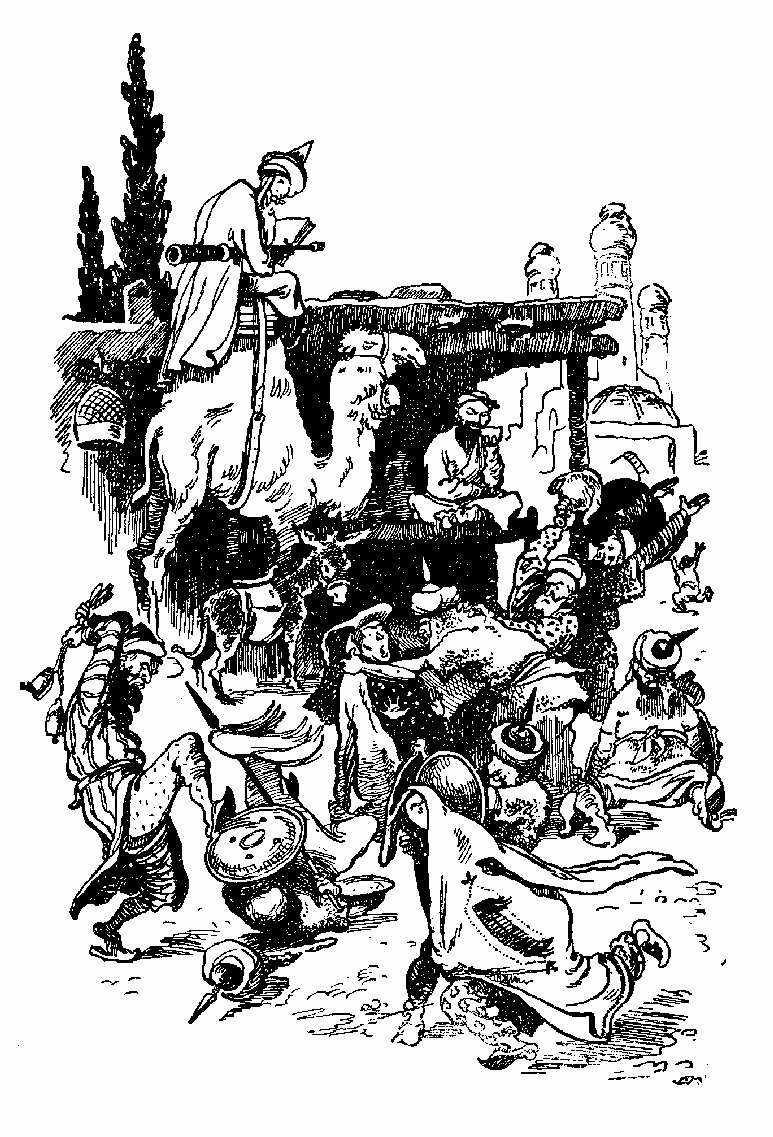
\includegraphics[width=\textwidth]{12.png}
\end{figure}

—~Да~будет известно тебе,~— с~важностью ответил старик, несколько уязвленный словами Ходжи Насреддина,~— что я~знаменитый мудрец, звездочет и~лекарь и~прибыл сюда из~самого Багдада по~приглашению эмира, дабы служить ему и~помогать в~правлении государством.

—~О! —~сказал Ходжа Насреддин, почтительно кланяясь,~— привет тебе, мудрый старец. Мне приходилось бывать в~Багдаде, и~я~знаю тамошних мудрецов. Скажи мне свое имя.

—~Если ты~был в~Багдаде, то, конечно, слышал обо мне и~моих заслугах перед калифом, которому спас я~от~смерти любимого сына, о~чем объявлено было по~всему государству. Гуссейн Гуслия~— мое имя.

—~Гуссейн Гуслия! —~воскликнул Ходжа Насреддин. —~Неужели ты~и~есть сам Гуссейн Гуслия!

Старик не~смог скрыть улыбки, весьма довольный тем, что слава его разнеслась так далеко за~пределы родного Багдада.

—~Чему ты~удивляешься? —~продолжал старик. —~Ну~да, я~и~есть тот самый знаменитый Гуссейн Гуслия, великий мудрец, равного которому нет ни~в~мудрости, ни~в~умении вычислять звезды, ни~в~искусстве излечивать болезни. Но~я~совершенно лишен гордости и~самодовольства~— видишь, как просто я~разговариваю с~тобой, ничтожным.

Старик придвинул подушку, облокотился на~нее, собравшись простереть далее свое снисхождение к~собеседнику и~подробно поведать ему о~своей великой мудрости~— в~расчете, что собеседник, движимый тщеславием, начнет потом на~всех перекрестках рассказывать о~встрече со~знаменитым мудрецом Гуссейном Гуслия, превозносить его мудрость и~даже преувеличивать, дабы вызвать у~слушателей еще больше почтения к~нему, а~тем самым и~уважения к~себе,~— потому что именно так поступают всегда все люди, удостоившиеся внимания высоких особ. «И~этим он~будет способствовать умножению и~укреплению моей славы среди простого народа,~— думал Гуссейн Гуслия,~— что тоже не~лишне; разговоры в~простом народе дойдут через шпионов и~соглядатаев до~слуха самого эмира и~подтвердят перед ним мою мудрость, ибо подтверждение со~стороны есть, бесспорно, самое лучшее подтверждение; и~в~конце концов, из~всего этого я~смогу извлечь для себя пользу».

Дабы окончательно убедить собеседника в~своей необыкновенной учености, мудрец начал рассказывать о~созвездиях, о~расположении~их, поминутно ссылаясь при этом на~великих мудрецов древности.

Ходжа Насреддин слушал внимательно, стараясь запомнить каждое слово.

—~Нет,~— сказал наконец Ходжа Насреддин. —~Я~все-таки не~могу поверить! Неужели ты~и~есть тот самый Гуссейн Гуслия!

—~Конечно! —~воскликнул старик. —~Что в~этом удивительного?

Ходжа Насреддин опасливо отодвинулся. Затем воскликнул с~тревогой и~состраданием в~голосе:

—~О~несчастный! Пропала твоя голова! Старик поперхнулся, выронил чашку. Это было как в~шахматной игре, в~которой, кстати, лишь очень немногие могли~бы потягаться с~Ходжой Насреддином.

Вся важность и~высокомерие слетели со~старика мигом.

—~Как? Что? Почему? —~спрашивал он~испуганно. Ходжа Насреддин указал на~площадь, где не~совсем еще затихло побоище:

—~Да~ты~разве не~знаешь, что все это смятение из-за тебя?! До~слуха сиятельного эмира дошло, что~ты, выезжая из~Багдада, всенародно поклялся проникнуть в~эмирский гарем~— о, горе тебе, Гуссейн Гуслия! —~и~обесчестить эмирских жен!

Челюсть мудреца отвисла, глаза побелели, он~начал часто икать от~страха...

—~Я? —~бормотал~он. —~Я~— в~гарем?..

—~Ты~поклялся в~этом подножием трона аллаха. Так объявили сегодня глашатаи. И~наш эмир велел схватить тебя, едва ты~вступишь в~город, и~немедля отрубить тебе голову.

Мудрец застонал в~изнеможении. Он~никак не~мог сообразить, кто из~его врагов ухитрился нанести ему такой удар; в~остальном~же он~не~усомнился, ибо сам в~придворной борьбе не~раз сокрушал своих врагов подобными способами и~с~удовлетворением любовался потом их~головами, торчащими на~шестах.

—~И~вот сегодня,~— продолжал Ходжа Насреддин,~— шпионы донесли эмиру, что ты~приехал, и~он~повелел схватить тебя. Стражники кинулись на~базар, начали всюду искать тебя, перерывать лавки, и~разрушилась торговля, и~возмутилось спокойствие; по~ошибке стражники схватили одного человека, похожего на~тебя, и~второпях отделили ему голову, а~он~оказался муллой, известным своим благочестием и~добродетели~ми, паства его мечети вознегодовала~— и~посмотри, что творится теперь по~твоей милости в~Бухаре!

—~О~я~несчастный! —~воскликнул мудрец в~ужасе и~отчаянии.

Он~принялся горестно восклицать, стонать и~жаловаться, из~чего Ходжа Насреддин заключил, что достиг полного успеха в~своем намерении.

Драка тем временем отодвинулась к~воротам дворца, куда один за~другим скрывались избитые и~помятые стражники, растерявшие свое оружие. Базар гудел, волновался, но~уже тише прежнего.

—~В~Багдад! —~стеная, восклицал мудрец. —~Обратно в~Багдад!

—~Но~тебя схватят у~городских ворот! —~возразил Ходжа Насреддин.

—~О~горе! О~великое бедствие! Аллах видит, что я~невинен; никогда и~никому я~не~давал столь дерзкой, столь нечестивой клятвы! Это мои враги оклеветали меня перед эмиром! Помоги мне, добрый мусульманин!

Ходжа Насреддин только этого и~ждал, ибо не~хотел первый предлагать мудрецу свою помощь, чтобы не~возбудить в~нем подозрений.

—~Помочь? —~сказал~он. —~Чем~же я~могу тебе помочь, не~говоря уже о~том, что~я, как преданный и~верный раб моего владыки, должен предать тебя без промедления в~руки стражников.

Мудрец, икая и~дрожа, устремил на~Ходжу Насреддина умоляющий взгляд.

—~Но~ты~говоришь, что тебя оклеветали невинно,~— поспешил успокоить его Ходжа Насреддин. —~Я~верю тебе, потому что ты~находишься в~столь преклонном возрасте, когда в~гареме нечего делать.

—~Справедливо! —~воскликнул старик. —~Но~существует~ли для меня путь к~спасению?

—~Существует,~— ответил Ходжа Насреддин, повел старика в~темную заднюю комнату чайханы и~там вручил ему узел с~женской одеждой. —~Я~купил это сегодня по~случаю для моей жены~и, если хочешь, могу обменять на~твой халат и~чалму. Под женским покрывалом ты~укроешься от~шпионов и~стражников.

Старик с~изъявлением восторга и~благодарности схватил женскую одежду, натянул на~себя. Ходжа Насреддин облачился в~его белый халат, надел его чалму с~подвернутым концом, опоясался широким поясом, покрытым изображением звезд. Старик предлагал обменять и~своего верблюда на~ишака, но~Ходжа Насреддин не~захотел расстаться со~своим верным другом.

Ходжа Насреддин помог старику взобраться на~верблюда:

—~Да~сохранит тебя аллах, о~мудрец! Не~забывай только, что со~всеми ты~должен говорить голосом тонким, как у~женщины.

Старик погнал верблюда крупной рысью. Глаза Ходжи Насреддина сияли. Путь во~дворец был открыт!..


\chapter{}

Убедившись, что драка на~площади затихает, сиятельный эмир решил выйти в~большой зал к~придворным. Он~придал своему лицу выражение хотя и~скорбное, но~спокойное, дабы кто-нибудь из~придворных не~дерзнул вдруг подумать, что страх имеет доступ к~царственному сердцу эмира.

Он~вышел, и~придворные замерли, трепеща перед мыслью, как~бы эмир по~их~глазам и~лицам не~угадал, что они знают о~подлинных его чувствах.

Эмир молчал, и~придворные молчали; царствовало грозное молчание.

Наконец эмир нарушил его:

—~Что вы~скажете нам и~что посоветуете? Уже не~в~первый раз мы~спрашиваем вас об~этом!

Никто не~поднял головы, не~ответил. Мгновенная молния передернула лицо эмира. И~неизвестно, сколько голов, увенчанных чалмами и~обрамленных седыми бородами, легли~бы сегодня на~плаху и~сколько льстивых языков, прокушенных в~предсмертной судороге насквозь, замолкли~бы навсегда, высунувшись из~посиневших уст, как~бы дразня живых, напоминая им~о~полной призрачности их~благополучия, о~тщете и~суете их~стремлений, хлопот и~надежд!

Но~все головы остались на~плечах, и~все языки остались пребывающими в~готовности к~немедленному льстивому действию~— потому что вошел дворцовый надзиратель и~возвестил:

—~Хвала средоточию вселенной! К~воротам дворца прибыл неизвестный человек, называющий себя Гус-сейном Гуслия, мудрецом из~Багдада. Он~объявил, что имеет важное дело и~должен немедленно предстать пред светлыми очами повелителя.

—~Гуссейн Гуслия! —~воскликнул эмир, оживившись. —~Пропустите его! Зовите его сюда!

Мудрец не~вошел, он~вбежал, не~скинув даже запыленных туфель, и~распростерся ниц перед троном.

—~Приветствую славного и~великого эмира, солнце и~луну вселенной, грозу и~благо~ее! Я~спешил день и~ночь" чтобы предупредить эмира о~страшной опасности. Пусть эмир скажет, не~входил~ли он~сегодня к~женщине. Пусть эмир ответит своему ничтожнейшему рабу, я~умоляю повелителя!..

—~К~женщине? —~озадаченно переспросил эмир. —~Сегодня?.. Нет... Мы~собирались, но~еще не~входили.

Мудрец поднялся. Лицо его было бледным. Он~ждал этого ответа в~страшном волнении. Глубокий, длительный вздох облегчил его грудь, и~румянец, медленно возвращаясь, начал окрашивать его щеки.

—~Слава всемогущему аллаху! —~воскликнул~он. —~Аллах не~дал погаснуть светочу мудрости и~милосердия! Да~будет известно великому эмиру, что вчера ночью планеты и~звезды расположились крайне неблагоприятно для него. И~я, ничтожный и~достойный лобызать лишь прах следов эмира, изучил и~вычислил расположение планет и~узнал, что пока не~станут они в~благоприятное и~благоденственное сочетание, эмир не~должен касаться женщины, иначе гибель его неминуема. Слава аллаху, что я~успел вовремя!

—~Подожди, Гуссейн Гуслия,~— остановил его эмир. —~Ты~говоришь что-то непонятное...

—~Слава аллаху, что я~успел вовремя! —~продолжал восклицать мудрец (это был, конечно. Ходжа Насреддин). —~Теперь я~буду до~конца дней моих гордиться тем, что помешал эмиру коснуться женщины и~не~допустил вселенную осиротеть.

Он~воскликнул с~такой радостью и~горячностью, что эмир не~мог не~поверить ему.

—~Когда~я, ничтожный муравей, был озарен лучами величия эмира, соизволившего вспомнить мое недостойное имя, и~получил повеление прибыть з~Бухару на~эмирскую службу, то~я~как~бы погрузился в~сладостное море небывалого счастья. И~я, конечно, выполнил без всяких задержек это повеление и~выехал тотчас~же, потратив только несколько дней на~составление гороскопа эмира, дабы, будучи в~пути, уже служить ему, наблюдая за~движением планет и~звезд, имеющих влияние на~его судьбу. И~вот вчера ночью, взглянув на~небо, я~увидел, что звезды расположились ужасно и~зловеще для эмира, а~именно: звезда Аль-Кальб, означающая жало, стала напротив звезды Аш-Шуала, которая означает сердце; далее увидел я~три звезды Аль-Гафр, означающие покрывало женщины, две звезды Аль-Иклиль, означающие корону, и~две звезды Аш-Шаратан, означающие рога. И~было это во~вторник~— день планеты Марса, а~день этот, в~противоположность четвергу, указывает на~смерть великих людей и~весьма неблагоприятен для эмиров. Сопоставив все эти признаки, понял~я, ничтожный звездочет, что жало смерти угрожает сердцу носящего корону, если он~коснется покрывала женщины, и, дабы предупредить носящего корону, я~спешил день и~ночь, загнал до~смерти двух верблюдов и~вошел пешком в~Бухару.

—~О~всемогущий аллах! —~произнес пораженный эмир. —~Неужели нам действительно угрожала такая страшная опасность! Но~может быть, ты~просто перепутал, Гуссейн Гуслия?

—~Я~перепутал? —~воскликнул мудрец. —~Да~будет известно эмиру, что нигде от~Багдада и~до~Бухары нет никого, равного мне в~мудрости, или в~умении вычислять звезды, или излечивать болезни! Я~не~мог перепутать. Пусть владыка и~сердце вселенной, великий эмир, спросит у~своих мудрецов, правильно~ли я~обозначил звезды и~справедливо~ли истолковал их~расположение в~гороскопе.

Мудрец с~искривленной шеей, повинуясь знаку эмира, выступил вперед:

—~Несравненный собрат мой по~мудрости Гуссейн Гуслия правильно назвал звезды, что доказывает познания его, усомниться в~которых никто не~осмелится. Но,~— продолжал мудрец, и~в~голосе его Ходжа Насреддин почувствовал коварство,~— почему мудрейший Гуссейн Гуслия не~назвал перед великим эмиром шестнадцатого стояния луны и~созвездия, на~которое это стояние приходится, ибо без этих обозначений неосновательным было~бы утверждать, что вторник~— день планеты Марса~— точно указывает на~смерть великих людей, в~том числе и~носящих корону, ибо планета Марс имеет дом в~одном созвездии, возвышение в~другом, падение в~третьем и~ущерб в~четвертом, и, в~соответствии с~этим, планета Марс имеет четыре разных указания, а~не~одно только, как сказал нам почтеннейший и~мудрейший Гуссейн Гуслия.

Мудрец умолк, и~на~губах его играла змеиная улыбка; придворные одобрительно зашептались, радуясь посрамлению вновь прибывшего. Оберегая свои доходы и~высокое положение, они старались никого со~стороны не~допускать во~дворец и~в~каждом новом человеке видели опасного соперника.

Но~Ходжа Насреддин если уж~за~что-нибудь брался, то~не~отступал никогда. Кроме того, он~насквозь видел и~мудреца, и~придворных, и~самого эмира. Нисколько не~смутившись, он~снисходительно ответил:

—~Может быть, мой почтенный и~мудрый собрат несравненно превосходит меня в~какой-либо другой области познаний, но~что касается звезд, то~он~обнаруживает своими словами полное незнакомство с~учением мудрейшего из~всех мудрых ибн-Баджжа, который утверждает, что планета Марс, имея дом в~созвездии Овна и~Скорпиона, возвышение~— в~созвездии Козерога, падение~— в~созвездии Рака и~ущерб~— в~созвездии Весов, тем не~менее всегда присуща только дню вторнику, на~который и~оказывает свое влияние, пагубное для носящих короны.

Отвечая, Ходжа Насреддин ничуть не~опасался быть уличенным в~невежестве, ибо отлично знал, что в~таких спорах побеждает всегда тот, у~кого лучше привешен язык, а~в~этом с~Ходжой Насреддином трудно было сравниться.

Он~стоял, ожидая возражений мудреца и~готовясь ответить достойно. Но~мудрец не~принял вызова. Он~промолчал. Хотя он~очень сильно подозревал Ходжу Насреддина в~мошенничестве и~невежестве, но~подозрение не~есть уверенность, можно и~ошибиться; зато о~своем крайнем невежестве мудрец знал точно и~не~осмелился спорить. Таким образом, его попытка посрамить вновь прибывшего послужила к~обратному. Придворные зашипели на~мудреца, и~он~пояснил глазами, что противник слишком опасен, чтобы схватиться с~ним открыто.

Все это, конечно, не~ускользнуло от~внимания Ходжи Насреддина. «Ну, подождите! —~думал~он. —~Вы~еще узнаете меня!»

Эмир погрузился в~глубокое раздумье. Никто не~шевелился из~опасения помешать ему.

—~Если все звезды названы и~обозначены тобою правильно, Гуссейн Гуслия,~— сказал эмир,~— тогда, действительно, толкование твое справедливо. Мы~только никак не~можем понять, почему в~наш гороскоп попали две звезды Аш-Шаратан, означающие рога? Ты~успел, поистине, вовремя, Гуссейн Гуслия! Только сегодня утром в~наш гарем привели одну девушку, и~мы~собирались...

Ходжа Насреддин в~притворном ужасе взмахнул руками.

—~Извергни ее~из~своих мыслей, пресветлый эмир, извергни~ее! —~вскричал~он, словно~бы позабыв, что к~эмиру нельзя обращаться прямо, но~лишь косвенно, в~третьем лице. При этом он~рассчитал, что такое нарушение правил, вызванное как~бы сильным душевным волнением, проистекающим из~преданности эмиру и~беспокойства за~его жизнь, не~только не~будет поставлено в~большую вину, но, наоборот, свидетельствуя об~искренности чувств восклицающего, еще больше возвысит его в~глазах эмира.

Он~так просил и~умолял эмира не~прикасаться к~девушке, дабы потом ему, Гуссейну Гуслия, не~проливать реки слез и~не~надевать черные одежды горя, что эмир даже растрогался.

—~Ну, успокойся, успокойся, Гуссейн Гуслия. Мы~не~враг нашему народу, чтобы оставить его осиротевшим и~утопающим в~скорби. Мы~обещаем тебе, в~заботе о~нашей драгоценной жизни, не~входить к~этой девушке и~вообще не~входить в~гарем, пока звезды не~изменят своего расположения, о~чем ты~нам своевременно скажешь. Подойди ближе.

С~этими словами он~сделал знак своему кальянщику и~потом собственноручно передал золотой чубук приезжему мудрецу, что было великой честью и~милостью. Преклонив колени и~опустив глаза, мудрец принял эмирскую милость, причем по~всему телу его прошла дрожь. («От~восторга!»~— как подумали придворные, снедаемые злобной завистью.)

—~Мы~объявляем нашу милость и~благоволение мудрецу Гуссейну Гуслия,~— сказал эмир,~— и~назначаем его самым главным мудрецом нашего государства, ибо его ученость, ум, а~равно великая преданность нам достойны всяческого подражания.

Придворный летописец, обязанностью которого было записывать в~хвалебных выражениях все поступки и~слова эмира, дабы его величие не~потускнело в~будущих веках (о~чем эмир заботился чрезвычайно), заскрипел тростниковым пером.

—~Вам~же,~— продолжал эмир, обращаясь к~придворным,~— мы, наоборот, изъявляем свое неудовольствие, ибо вашему повелителю после всех неприятностей, причиненных Ходжой Насреддином, грозила еще и~смерть, но~вы~даже не~почесались! Посмотри на~них, Гуссейн Гуслия, посмотри на~этих болванов, на~их~морды, вполне подобные ишачьим! Поистине, еще ни~один государь никогда не~имел столь глупых и~нерадивых визирей!

—~Светлейший эмир совершенно прав,~— сказал Ходжа Насреддин, обводя взглядом безмолвствующих придворных и~как будто прицеливаясь, чтобы нанести первый удар. —~Лица этих людей, как я~вижу, не~отмечены печатью мудрости!

—~Вот, вот! —~обрадовался эмир. —~Вот именно~— не~отмечены печатью мудрости!

—~Скажу еще,~— продолжал Ходжа Насреддин,~— что я~равным образом не~вижу здесь лиц, отмеченных печатью добродетели и~честности.

—~Воры! —~сказал эмир убежденно. —~Все воры! Все до~единого! Поверишь~ли, Гуссейн Гуслия, они обкрадывают нас денно и~нощно! Нам приходится самолично следить за~каждой мелочью во~дворце, и~каждый раз, проверяя дворцовое имущество, мы~чего-нибудь недосчитываемся. Не~далее как сегодня утром в~саду мы~позабыли наш новый шелковый пояс, а~через полчаса его уж~там не~было!.. Кто-то из~них успел... ты~понимаешь, Гуссейн Гуслия!..

При этих словах мудрец с~искривленной шеей как-то по-особенному кротко и~постно потупил глаза. В~другое время это движение осталось~бы незамеченным, но~сегодня все чувства Ходжи Насреддина были обострены: он~все замечал и~сразу обо всем догадывался.

Он~уверенно подошел к~мудрецу, запустил руку к~нему за~пазуху и~вытащил оттуда шелковый, богато расшитый пояс:

—~Не~об~этом~ли поясе сожалел великий эмир?

Изумление и~ужас сковали придворных. Новый мудрец оказался действительно опасным соперником, и~первый~же, выступивший против него, был уже сокрушен им~и~повергнут в~прах. У~многих мудрецов, поэтов, сановников и~визирей дрогнули сердца в~этот миг.

\begin{figure}[h]
\centering
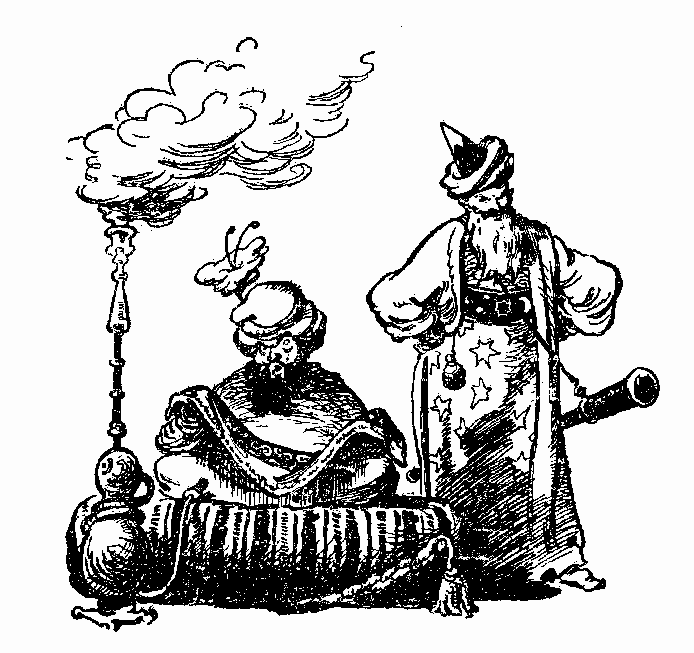
\includegraphics[width=\textwidth]{13.png}
\end{figure}

—~Клянусь аллахом, это тот самый пояс! —~вскричал эмир. —~Гуссейн Гуслия, ты, воистину, несравненный мудрец! Ага! —~торжествующе обратился эмир к~придворным, причем лицо его выражало самую искреннюю, живую радость. —~Попались наконец! Теперь-то вы~уж~не~сможете украсть у~нас ни~одной нитки; довольно мы~натерпелись от~вашего воровства! А~этому презренному вору, дерзко похитившему наш пояс, выщипать все волосы на~голове, подбородке и~на~теле и~дать ему по~его подошвам сотню палок, и~посадить его, голого, на~осла лицом к~хвосту, и~возить его по~городу, объявляя повсеместно, что он~вор!

По~знаку Арсланбека палачи накинулись на~мудреца и~вытолкнули за~дверь; там, прямо на~пороге, закипела работа; через две минуты палачи втолкнули мудреца обратно в~зал, голого, лишенного даже волос, срамного донельзя. Тут всем стало ясно, что до~сих пор только его борода и~огромная чалма скрывали убожество ума и~клеймо порока, лежавшее на~его лице, что человек с~таким шельмовским лицом не~может быть никем иным, кроме как наиотъявленнейшим плутом и~вором.

Эмир поморщился:

—~Уберите!

Палачи потащили мудреца, и~вскоре за~окном послышались его вопли, сопровождаемые сочными ударами палок по~пяткам.

Потом его посадили голого на~осла, лицом к~хвосту, и~под ужасающий рев труб, под грохот барабанов повезли на~базарную площадь.

Эмир долго беседовал с~приезжим мудрецом. Придворные стояли не~шевелясь, что было для них крайне мучительно: жара усиливалась, потные спины под халатами чесались невыносимо. Великий визирь Бахтияр, больше всех опасавшийся нового мудреца, был занят мыслями о~привлечении придворных на~свою сторону, чтобы сокрушить с~их~помощью соперника; придворные~же, заранее угадывая по~многим признакам исход борьбы, рассчитывали, как~бы повыгоднее отречься в~решительную минуту от~Бахтияра, предать его и~тем самым войти в~доверие и~милость к~новому мудрецу.

А~эмир все расспрашивал о~здоровье калифа, о~багдадских новостях, о~событиях в~пути. Ходже Насреддину пришлось по-всякому изворачиваться. И~все уже сошло благополучно, и~эмир, утомленный беседой, приказал приготовить себе ложе для отдыха, но~вдруг за~открытыми окнами послышались голоса, чей-то вопль.

В~зал быстрыми шагами вошел дворцовый надзиратель. Его лицо сияло радостью. Он~объявил:

—~Да~будет известно великому повелителю, что богохульник и~возмутитель спокойствия Ходжа Насреддин пойман и~приведен во~дворец!

Сразу~же вслед за~этими словами широко раскрылись ореховые резные двери. Стражники, торжествующе громыхая оружием, ввели горбоносого седобородого старика в~женской одежде и~повергли его на~ковры перед троном.

Ходжа Насреддин похолодел, стены дворца словно~бы покачнулись перед его глазами, лица придворных окутались зеленоватым туманом...


\chapter{}

Багдадский мудрец, подлинный Гуссейн Гуслия, попался у~самых ворот, за~которыми уже видел он~сквозь свое покрывало поля и~дороги, разбегающиеся в~разные стороны; каждая из~них обещала ему избавление от~страшной казни.

Но~стражники, охранявшие в~этот час городские ворота, окликнули:

—~Куда едешь~ты, женщина?

Мудрец ответил голосом молодого осипшего петуха:

—~Я~тороплюсь домой к~мужу. Пропустите меня, доблестные воины.

Стражники переглянулись~— голос показался им~подозрительным. Один из~них взял под узцы верблюда.

—~Где ты~живешь?

—~Вот здесь, неподалеку,~— ответил мудрец еще тоньше. Но~при этом чрезмерно задержал воздух в~гортани и~закашлялся с~ужасным хрипом и~одышкой.

Тогда стражники сорвали с~него чадру. Ликование их~было безгранично.

—~Вот он! Вот он! —~кричали они. —~Давай, вяжи! Хватай!

Потом они повели старика во~дворец, всю дорогу беседовали о~казни, ожидающей его, о~трех тысячах таньга награды за~его голову. Каждое слово стражников падало как раскаленный уголь на~его сердце.

Он~лежал перед троном, горько рыдая, умоляя о~помиловании.

—~Поднять его! —~приказал эмир. Стражники подняли старика. Из~толпы придворных выступил Арсланбек:

—~Пусть выслушает эмир слово преданного раба своего. Это не~Ходжа Насреддин, это совсем другой человек: Ходже Насреддину нет еще и~сорока лет, а~это~— глубокий старик.

Стражники встревожились: награда уплывала у~них из~рук. Все остальные молчали в~недоумении.

—~Почему ты~скрывался под женской одеждой? —~грозно вопросил эмир.

—~Я~ехал во~дворец к~великому и~всемилостивейшему эмиру,~— ответил старик дрожа. —~Но~со~мной повстречался какой-то человек, неизвестный мне, и~сказал, что эмир еще до~моего появления в~Бухаре издал приказ, чтобы отрубить мне голову, и~я, обуянный страхом, решил бежать под женской одеждой.

Эмир проницательно усмехнулся:

—~С~тобой повстречался человек... Неизвестный тебе. И~ты~сразу ему поверил?.. Удивительная история! За~что~же мы~хотели отрубить тебе голову?

—~За~то, что я~будто~бы всенародно поклялся проникнуть в~гарем великого эмира... Но, аллах свидетель, я~никогда не~думал об~этом! Я~уже стар, немощен и~даже от~собственного своего гарема давно отказался...

—~Проникнуть в~наш гарем? —~переспросил эмир, поджав губы. По~его лицу было видно, что этот старик становится ему все более и~более подозрителен. —~Кто ты~и~откуда~ты?

—~Я~Гуссейн Гуслия, мудрец, звездочет и~лекарь из~Багдада и~приехал в~Бухару по~повелению и~желанию великого эмира!..

—~Значит, твое имя Гуссейн Гуслия! Ты~лжешь в~глаза нам, презренный старик! —~загремел эмир с~такой силой, что царь поэтов совсем некстати повалился на~колени. —~Ты~лжешь! Вот Гуссейн Гуслия!

Ходжа Насреддин, повинуясь знаку эмира, бестрепетно вышел вперед и~стал перед стариком, открыто и~смело глядя прямо в~лицо ему.

Старик изумился и~попятился. Но~тут~же, овладев собой, закричал:

—~Ага! Да~ведь это тот самый человек, который, повстречавшись со~мной на~базаре, сказал, что эмир хочет отрубить мне голову!

—~Что он~говорит, Гуссейн Гуслия! —~воскликнул эмир в~полном недоумении.

—~Какой он~Гуссейн Гуслия! —~завопил старик. —~Это я~— Гуссейн Гуслия, а~он~просто обманщик! Он~присвоил себе мое имя!

Ходжа Насреддин низко поклонился эмиру:

—~Да~простит мне великий владыка мое смелое слово, но~бесстыдство этого старика не~имеет пределов! Он~говорит, что я~присвоил себе его имя. Он, может быть, скажет, что этот халат я~тоже присвоил?

—~Конечно! —~закричал старик. —~Это мой халат!

—~Может быть, и~эта чалма твоя? —~спросил Ходжа Насреддин с~насмешкой в~голосе.

—~Ну~да! Это моя чалма! Ты~выменял у~меня и~халат и~чалму на~женскую одежду!

—~Так! —~сказал Ходжа Насреддин с~еще большей насмешкой в~голосе. —~А~вот этот пояс случайно не~твой?

—~Мой пояс! —~запальчиво ответил старик. Ходжа Насреддин повернулся к~трону:

—~Пресветлый владыка эмир воочию убедился, кого видит он~перед собой. Сегодня этот лживый и~презренный старик говорит, что я~присвоил себе его имя, что этот халат~— его халат, и~чалма его, и~пояс его, а~завтра он~скажет, что этот дворец~— его дворец, и~все государство~— его государство, и~что настоящий эмир Бухары не~наш великий и~солнцеподобный владыка, восседающий сейчас перед нами на~троне, а~что настоящий эмир~— это~он, вот этот лживый, презренный старик! От~него можно всего ожидать! Ведь он~уже приехал в~Бухару с~намерением войти в~эмир-ский гарем, как в~собственный свой гарем!..

—~Ты~прав, Гуссейн Гуслия,~— сказал эмир. —~Мы~убедились, что этот старик~— подозрительный и~опасный человек, у~него в~голове черные мысли. И~мы~считаем, что нужно немедленно отделить его голову от~его туловища.

Старик со~стоном упал на~колени, закрыл руками лицо.

Но~Ходжа Насреддин не~мог допустить, чтобы из-за него пошел на~плаху человек, неповинный в~тех преступлениях, которые ему приписывали, хотя~бы то~был и~придворный мудрец, сам, конечно, погубивший многих и~многих своим коварством.

Ходжа Насреддин поклонился эмиру:

—~Да~выслушает милостиво великий эмир мое слово. Отрубить голову ему~— никогда не~поздно. Но~сначала нужно узнать его подлинное имя и~подлинные намерения, с~которыми он~прибыл в~Бухару, дабы выяснить, нет~ли у~него сообщников и~не~гнусный~ли он~чернокнижник, решивший воспользоваться неблагоприятным расположением звезд и~добыть прах от~следов великого эмира, смешать этот прах с~мозгами летучей мыши и~затем подбросить в~кальян эмиру, дабы причинить ему зло. Пусть великий эмир оставит его пока живым и~отдаст мне, ибо обычных тюремщиков он~может опутать своими злыми чарами, но~перед моею мудростью они будут бессильны, так как мне известны все ухищрения чернокнижников и~все способы уничтожения их~колдовства. Я~запру этого старика, произнесу над замком благочестивые молитвы, известные только мне одному,~— дабы не~смог он~силой колдовства открыть замок без ключа,~— и~потом жестокими пытками я~заставлю его сказать все!

—~Ну~что~же,~— ответил эмир. —~Твои слова вполне разумны, Гуссейн Гуслия. Бери его и~делай с~ним, что захочешь, но~только смотри, чтобы он~не~вырвался из-под замка.

—~Я~отвечаю головой перед великим эмиром.

Через полчаса Ходжа Насреддин~— он~же главный мудрец и~звездочет эмира~— проследовал в~свое новое жилище, приготовленное в~одной из~башен дворцовой стены; за~ним, сопровождаемый стражниками, следовал понурившийся преступник~— подлинный Гуссейн Гуслия.

В~башне, над жилищем Ходжи Насреддина, была маленькая круглая келья с~чугунной решеткой в~окне. Ходжа Насреддин отпер огромным ключом медный, позеленевший замок, открыл окованную железом дверь. Стражники втолкнули туда старика, бросив ему тощую охапку соломы. Ходжа Насреддин закрыл дверь и~потом долго бормотал над медным замком, но~так невнятно и~быстро, что стражники не~могли ничего разобрать, кроме часто повторяющегося призыва к~аллаху...

Своим жилищем Ходжа Насреддин остался вполне доволен. Эмир прислал ему двенадцать одеял, восемь подушек, множество разной утвари, корзину с~белыми свежими лепешками, мед в~кувшине и~много других яств со~своего стола. Ходжа Насреддин очень устал и~проголодался, но~прежде чем сесть за~трапезу, он~взял шесть одеял, четыре подушки и~понес все это наверх своему пленнику.

Старик сидел в~углу на~соломе и~сверкал из~темноты глазами, как разъяренный кот.

—~Ну~что~же, Гуссейн Гуслия,~— мирно сказал Ходжа Насреддин. —~Мы~с~тобой неплохо устроимся в~этой башне~— я~пониже, а~ты~повыше, как тебе и~подобает по~твоим годам и~мудрости. Сколько здесь пыли! Я~сейчас подмету.

Ходжа Насреддин спустился, принес кувшин с~водой, веник, чисто вымел каменный пол, постелил одеяла, положил подушки, потом еще раз спустился, принес лепешки, мед, халву, фисташки и~на~глазах своего пленника честно разделил все пополам.

—~Ты~не~умрешь с~голоду, Гуссейн Гуслия,~— говорил~он. —~Мы~с~тобой сумеем раздобыть пищу. Вот тебе кальян, а~вот здесь я~положил табак.

Устроив все это в~маленькой келье так, что она имела вид едва~ли не~лучший, чем нижняя. Ходжа Насреддин ушел, заперев дверь на~замок.

Старик остался один. Он~был в~полной растерянности. Он~долго думал, соображая, прикидывая, но~так и~не~смог ничего понять в~происходящем. Одеяла были мягкими, и~подушки удобными, и~ни~лепешки, ни~мед, ни~табак не~содержали в~себе отравы... Утомленный сегодняшними треволнениями, старик улегся спать, поручив свою дальнейшую судьбу аллаху.

В~это время виновник всех его несчастий Ходжа Насреддин сидел в~нижней келье перед окном, наблюдал медленный переход сумерек в~темноту и~раздумывал о~своей удивительной бурной жизни и~возлюбленной, которая теперь была здесь, рядом, но~ничего еще пока не~знала. В~окно тянуло свежей прохладой, сплетались над городом, как серебряные нити, звенящие и~печальные голоса муэдзинов; на~темном небе выступили звезды, сияли, горели и~трепетали чистым, холодным, далеким огнем, и~была там звезда Аш-Шуале, означающая сердце, и~три звезды Аль-Гафр, означающие покрывало девушки, и~две звезды Аш-Шаратан, означающие рога, и~только зловещей звезды Аль-Кальб, означающей жало смерти, не~было там, в~синей высоте...


\part{}


\begin{quote}
Слава живому, который не~умирает!
\flushright{\textit{«Тысяча и~одна ночь»}}
\end{quote}

\chapter{}

Ходжа Насреддин вошел в~доверие и~милость к~эмиру, стал его ближайшим советником во~всех делах. Ходжа Насреддин решал, эмир подписывал, а~великий визирь Бахтияр только прикладывал медную резную печать. «О~великий аллах, да~это что~же творится в~нашем государстве! —~мысленно восклицал~он, читая эмирские указы об~отменах налогов, о~бесплатном пользовании дорогами и~мостами, об~уменьшении базарных сборов. —~Ведь так недолго совсем разорить казну! Этот новый мудрец, да~прогниют насквозь его внутренности, разрушил в~одну неделю все, над чем я~трудился больше десяти лет!»

Однажды он~осмелился доложить о~своих сомнениях эмиру. Повелитель ответил:

—~Что знаешь~ты, ничтожный, и~что понимаешь? Мы~сами не~меньше тебя скорбим об~этих указах, опустошающих нашу казну, но~что можем мы~сделать, если так повелевают звезды! Утешься, Бахтияр, это~— на~короткое время, пока звезды не~станут в~благоприятное сочетание. Объясни ему, Гуссейн Гуслия.

Ходжа Насреддин отвел великого визиря в~сторону, усадил на~подушки и~долго объяснял, почему дополнительный налог на~кузнецов, медников и~оружейников следует немедленно отменить.

—~Звезды Аль-Авва в~созвездии Девы и~Аль-Бальда в~созвездии Стрельца противостоят звездам Сад-Була в~созвездии Водолея,~— говорил Ходжа Насреддин. —~Ты~понимаешь, о~почтенный и~сиятельнейший визирь, они противостоят и~далеки от~сочетания.

—~Ну~и~что~же, если они противостоят? —~возразил Бахтияр. —~Они и~раньше противостояли, что, однако, ничуть не~мешало нам исправно взыскивать налоги.

—~Но~ты~позабыл о~звезде Ак-Дабаран в~созвездии Вола! воскликнул Ходжа Насреддин. —~О~визирь, посмотри на~небо, и~ты~убедишься!

—~Зачем мне смотреть на~небо! —~ответил упрямый визирь. —~Мое дело~— следить за~сохранностью и~приумножением казны; я~вижу, что с~того дня, как появился ты~во~дворце, доходы казны уменьшились и~приток налогов сократился. Сейчас как раз подошел срок взыскания налогов с~городских ремесленников; объясни мне, почему мы~не~можем взыскать?

—~Как почему? —~воскликнул Ходжа Насреддин. —~Да~я~же целый час толкую тебе об~этом! Неужели ты~до~сих пор не~понял, что на~каждый из~двенадцати знаков Зодиака выпадают два стояния луны с~одной третью!..

—~Но~я~должен взыскать налоги! —~снова перебил визирь. —~Ты~понимаешь, налоги!

—~Подожди,~— остановил его Ходжа Насреддин. —~Я~еще не~разъяснил тебе, что созвездие Ас-Сурейя и~восемь звезд Ан-Наими...

Здесь Ходжа Насреддин пустился в~столь туманные и~пространные объяснения, что в~голове у~великого визиря загудело и~в~глазах помутилось. Ой~встал и~вышел, пошатываясь. А~Ходжа Насреддин вернулся к~эмиру:

—~О~повелитель! Старость хотя и~покрыла серебром его голову, но~обогатила ее~лишь снаружи, не~превратив в~золото~то, что находится внутри головы. Он~не~смог вместить в~себя мою мудрость. Он~ничего не~понял, повелитель. О, если~бы он~обладал одною лишь тысячной долей того ума, которым обладает великий эмир, затмевающий самого Лухмана!

Эмир милостиво и~самодовольно улыбнулся. Все эти дни Ходжа Насреддин с~великим усердием внушал ему мысль о~его несравненной мудрости и~преуспел в~своем намерении вполне. И~теперь, когда он~доказывал что-нибудь эмиру, тот слушал с~глубокомысленным видом и~не~возражал, боясь обнаружить истинную глубину своего ума.

На~следующий день Бахтияр говорил в~кругу придворных:

—~Новый мудрец, этот самый Гуссейн Гуслия, разорит нас всех! Все мы~обогащаемся только в~дни собирания налогов, когда нам удается зачерпнуть из~большой и~полноводной реки, текущей в~эмирскую казну. И~вот пришло нам время зачерпнуть, но~этот Гуссейн Гуслия мешает. Он~ссылается на~расположение звезд, но~когда и~кто слышал, чтобы звезды, управляемые аллахом, располагались~бы в~ущерб знатным и~благородным людям, благоприятствуя в~то~же время каким-то презренным ремесленникам, которые~— я~уверен~— бесстыдно прожирают сейчас свои заработки, вместо того чтобы отдать их~нам! Когда и~кто слышал о~таком расположении звезд? Этого не~сказано ни~в~одной книге, потому что такая книга, если~бы даже и~появилась, то~была~бы немедленно сожжена, а~человек, сочинивший~ее, был~бы проклят и~предан казни, как величайший богохульник, еретик и~злодей!

Придворные молчали, еще не~зная, на~чью сторону выгоднее им~стать~— на~сторону Бахтияра или нового мудреца.

—~Уже сейчас приток налогов уменьшается с~каждым днем,~— продолжал Бахтияр. —~И~недалеко то~время, когда оскудеет казна, и~мы, приближенные эмира, разоримся, и~вместо парчовых халатов мы~наденем простые, грубые, и~вместо двадцати жен мы~будем довольствоваться только двумя, и~вместо серебряных блюд нам подадут глиняные, и~вместо нежного молодого барашка мы~положим в~плов жесткую говядину, пригодную лишь для собак и~ремесленников! Вот что готовит нам новый мудрец Гуссейн Гуслия, и~тот, кто этого не~видит, тот слеп, и~горе тому!

Так он~говорил, стараясь возмутить придворных против нового мудреца.

Напрасны были его усилия.

Гуссейн Гуслия все более и~более преуспевал в~своем возвышении.

Особенно~же отличился он~в~«день восхваления». По~стародавнему обычаю все визири, вельможи, мудрецы и~поэты ежемесячно соревновались перед лицом эмира в~наилучшем восхвалении его. Победителю выдавалась награда.

Все высказали свои похвалы, но~эмир остался недоволен.

—~То~же самое вы~говорили нам и~в~прошлый раз,~— сказал~он. —~И~мы~находим, что вы~недостаточно усердны в~славословии. Вы~не~желаете утруждать свой~ум, но~мы~заставим вас потрудиться сегодня. Мы~будем задавать вам вопросы, а~вы~должны отвечать, сочетая в~своих ответах восхваление с~правдоподобием.

Эмир спросил:

—~Если~мы, великий эмир бухарский, согласно вашим утверждениям, могуч и~непобедим, то~почему государи сопредельных мусульманских стран до~сих пор не~прислали к~нам своих послов с~богатыми подарками и~с~изъявлениями своей полной покорности нашему непреоборимому владычеству? Мы~ждем ваших ответов на~этот вопрос.

Полная растерянность охватила придворных. Они бормотали что-то невнятное, всячески старались уклониться от~прямого ответа. Один только Ходжа Насреддин сохранял уверенное спокойствие. Когда очередь дошла до~него, он~сказал:

—~Да~удостоятся мои жалкие слова внимания великого эмира. На~вопрос нашего владыки ответить легко. Все прочие государи, управляющие сопредельными странами, пребывают в~постоянном страхе и~трепете перед всемогуществом нашего владыки. И~рассуждают они таким образом: «Если пошлем мы~великому, славному и~могучему эмиру бухарскому богатые подарки, то~он~подумает, что земля наша очень богата, и, соблазнившись, придет со~своим войском и~заберет нашу землю. Если~же, наоборот, мы~пошлем ему подарки беднее, то~он~оскорбится и~все равно двинет на~нас свое войско. Он, эмир бухарский, велик, славен и~могуч, и~лучше всего не~напоминать ему о~нашем существовании». Вот как рассуждают прочие государи, и~причину того, что они не~присылают в~Бухару послов с~богатыми подарками, нужно искать в~их~беспрерывном трепете перед всемогуществом нашего владыки.

—~Вот! —~вскричал эмир, приведенный в~полное восхищение ответом Ходжи Насреддина. —~Вот как надо отвечать на~вопросы эмира! Вы~слышали! Учитесь, о~болваны, подобные чурбакам! Поистине, Гуссейн Гуслия превосходит вас всех своей мудростью в~десять раз! Объявляем ему свое благоволение.

Сейчас~же дворцовый повар подбежал к~Ходже Насреддину и~набил ему полный рот халвой и~леденцами. Щеки Ходжи Насреддина раздулись, он~задыхался, густая сладкая слюна текла по~его подбородку.

Эмир задал еще несколько столь~же коварных вопросов. Ответы Ходжи Насреддина были каждый раз наилучшими.

—~В~чем состоит наипервейшая обязанность придворного? -спросил эмир.

Ходжа Насреддин ответил ему так:

—~О~великий и~блистательный повелитель! Наипервейшая обязанность придворного состоит в~каждодневном упражнении спинного хребта, дабы последний приобрел необходимую гибкость, без чего придворный не~может достойным образом выразить свою преданность и~свое благоговение. Спинной хребет придворного должен обладать способностью изгибаться, а~также извиваться во~всех направлениях, в~отличие от~окостеневшего хребта какого-нибудь простолюдина, который даже и~поклониться не~умеет как следует.

—~Вот именно! —~вскричал восхищенный эмир. —~Вот именно, в~каждодневном упражнении спинного хребта! Вторично объявляем наше благоволение мудрецу Гуссейну Гуслия!

Ходже Насреддину во~второй раз набили рот халвой и~леденцами.

В~этот день многие из~придворных перешли от~Бахтияра на~сторону Ходжи Насреддина.

Вечером Бахтияр позвал к~себе Арсланбека. Новый мудрец равно угрожал им~обоим, и~ради его сокрушения они позабыли на~время старинную вражду.

—~Хорошо~бы подсыпать ему чего-нибудь в~плов,~— сказал Арсланбек, который был мастер на~такие дела.

—~А~потом эмир снимет нам головы! —~возразил Бахтияр. —~Нет, почтенный Арсланбек, действовать нужно иначе. Мы~должны всячески восхвалять и~превозносить мудрость Гуссейна Гуслия и~добиться того, чтобы в~сердце эмира закралось сомнение~— не~превосходит~ли в~глазах придворных мудрость Гуссейна Гуслия его собственную, эмирскую мудрость. А~мы~будем неустанно восхвалять и~превозносить Гуссейна Гуслия, и~наступит день, когда эмир возревнует. И~этот день для Гуссейна Гуслия будет последним в~его возвышении и~первым в~его падении!

Но~судьба заботливо оберегала Ходжу Насреддина, и~даже промахи его оборачивала на~пользу ему.

Когда Бахтияр и~Арсланбек, каждодневно и~неумеренно восхваляя нового мудреца, почти добились соединенными усилиями своей цели и~эмир, пока еще тайно, но~уже начал ревновать, случилось так, что Ходжа Насреддин промахнулся.

Они гуляли с~эмиром в~саду, вдыхая благоухание цветов и~наслаждаясь пением птиц. Эмир был молчалив. В~этом молчании Ходжа Насреддин чувствовал скрытую неприязнь, но~причины понять не~мог.

—~А~как твой пленник, этот самый старик? —~спросил эмир. —~Узнал~ли ты, Гуссейн Гуслия, его настоящее имя и~намерения, с~которыми он~прибыл в~Бухару?

Ходжа Насреддин думал в~это время о~Гюльджан и~ответил рассеянно:

—~Да~простит великий повелитель ничтожного раба своего. Я~не~мог добиться от~этого старика ни~одного слова. Он~молчит как рыба.

—~Но~ты~пробовал применить к~нему пытку?

—~О~великий повелитель, еще~бы! Позавчера я~выламывал ему суставы, а~вчера я~целый день железными клещами расшатывал ему зубы.

—~Это хорошая пытка, расшатывать зубы,~— сказал эмир. -Странно, что он~молчит. Может быть, прислать тебе на~помощь искусного и~опытного палача?

—~О~нет, пусть великий повелитель не~утруждает себя заботами! Завтра я~применю новую пытку~— я~буду пронзать язык и~десны этого старика раскаленным шилом.

—~Погоди, погоди! —~воскликнул эмир, и~лицо его просияло. —~Но~как он~тогда сможет назвать свое имя, если ты~пронзишь ему раскаленным шилом язык? Ты~не~подумал об~этом, Гуссейн Гуслия, и~не~предусмотрел, но~мы, великий эмир, подумали, предусмотрели и~предотвратили твою ошибку, из~чего видно, что хотя ты~и~несравненный мудрец, но~наша мудрость многократно превосходит твою, в~чем ты~сейчас убедился.

Радостный, сияющий эмир повелел немедленно созвать придворных, а~когда они собрались, объявил~им, что сегодня превзошел своею мудростью Гуссейна Гуслия, предотвратив ошибку, которую мудрец был готов совершить.

Придворный летописец старательно записал каждое слово эмира, дабы прославить мудрость его в~последующих веках.

С~этого дня ревность покинула сердце эмира.

Так, благодаря случайному промаху. Ходжа Насреддин разрушил коварные замыслы своих врагов.

Но~бывали у~него, и~все чаще, ночные одинокие часы невыносимого томления. Полная луна стояла высоко над Бухарой; слабым сиянием светились изразцовые шапки бесчисленных минаретов, а~мощные каменные подножия тонули в~глубоком дыму. Летел ветерок, прохладный над кровлями и~душный внизу, где земля и~стены, раскалившись днем, не~остывали за~ночь. Все вокруг спало~— дворец, мечети, хижины, только сова тревожила пронзительными криками горячую дрему священного города. Ходжа Насреддин сидел у~открытого окна. Сердцем он~знал, что Гюльджан не~спит, думает о~нем, и, может быть, оба они смотрят сейчас на~один и~тот~же минарет-, но~друг друга не~видят, разделенные стенами, решетками, стражей, евнухами и~старухами. Ходжа Насреддин сумел отомкнуть ворота дворца, но~гарем по-прежнему был заперт наглухо, только случай мог открыть его перед Ходжой Насреддином. Он~неутомимо искал этот случай. Тщетно!.. Он~даже не~смог до~сих пор послать Гюльджан весточку о~себе.

Он~сидел у~окна, целовал ветер и~говорил ему: «Ну~что тебе стоит! Залети на~минутку в~ее~окно, коснись ее~губ. Передай Гюльджан мой поцелуй и~мой шепот, скажи, что я~не~забыл~ее, что я~спасу~ее!» Ветер пролетал дальше. Ходжа Насреддин опять оставался наедине со~своей тоской.

Наступал день, а~с~ним~— обычные хлопоты и~заботы. Опять нужно было идти в~большой зал, там ждать выхода эмира, слушать льстивые слова придворных, отгадывать хитрые подкопы Бахтияра, ловить его взгляды, полные затаенного яда. Потом нужно было падать ниц перед эмиром, произносить ему восхваление, потом долгие часы сидеть с~ним вдвоем, смотреть, скрывая отвращение, на~его одутловатое, помятое лицо, слушать со~вниманием его глупые речи, объяснять ему расположение звезд. Все это до~того надоело и~опротивело Ходже Насреддину, что он~даже перестал придумывать для эмира новые доказательства, и~все подряд~— головную боль эмира, недостаток воды на~полях, повышение цен на~пшеницу,~— все объяснял одними и~теми~же словами, ссылаясь на~одни и~те~же звезды.

—~Звезды Сад-ад-Забих,~— говорил он~скучным голосом,~— противостоят созвездию Водолея, в~то~время как планета Меркурий стала слева от~созвездия Скорпиона. Этим и~объясняется сегодня бессонница повелителя.

—~Звезды Сад-ад-Забих противостоят планете Меркурию, в~то~время как... Это надо запомнить... Повтори, Гуссейн Гуслия.

Памяти у~великого эмира не~было никакой. На~следующий день разговор начинался снова:

—~Падеж скота в~горных местностях объясняется тем, о~великий эмир, что звезды Сад-ад-Забих встали в~сочетание с~созвездием Водолея, в~то~время как планета Меркурий противостоит созвездию

Скорпиона.

—~Значит, звезды Сад-ад-Забих,~— говорил эмир. —~Это надо запомнить.

«Всемогущий аллах, до~чего он~глуп! —~с~тоской думал Ходжа Насреддин. —~Он~еще глупее калифа багдадского! До~чего он~мне надоел, I/~скоро~ли я~вырвусь отсюда!»

А~эмир начинал новые речи:

—~В~нашем государстве, Гуссейн Гуслия, царят сейчас полный мир и~успокоение. И~даже ничего не~слышно об~этом нечестивце, о~Ходже Насреддине. Куда~бы он~мог деваться, и~почему он~молчит? Объясни нам, Гуссейн Гуслия.

—~О~всемогущий владыка, средоточие вселенной! Звезды Сад-ад-Забих... —~начинал скучным и~тягучим голосом Ходжа Насреддин и~снова повторял все, сказанное уже много раз. —~А~кроме того, великий эмир, этот нечестивец Ходжа Насреддин бывал в~Багдаде~и, конечно, слышал о~моей мудрости. Когда стало ему известно, что я~приехал в~Бухару, то~он~затаился, объятый страхом и~трепетом, ибо он~знает, что мне ничего не~стоит его поймать.

—~Поймать! Это было~бы очень хорошо! Но~каким способом думаешь ты~поймать его?

—~Я~для этого выжду благоприятного сочетания звезд Сад-ад-Забих с~планетой Юпитером.

—~С~планетой Юпитером,~— повторял эмир. —~Это надо запомнить. Знаешь~ли, Гуссейн Гуслия, какая мудрая мысль осенила нас сегодня ночью? Мы~подумали, что Бахтияра следует прогнать с~его должности, а~великим визирем поставить тебя.

И~надо было падать ниц перед эмиром, восхвалять и~благодарить его, а~потом объяснять, что сейчас нельзя производить смену визирей, ибо звезды Сад-ад-Забих не~благоприятствуют этому. «Скорее, скорее вырваться отсюда!»~— восклицал мысленно Ходжа Насреддин.

Так, поджидая случая. Ходжа Насреддин влачил во~дворце безрадостное, тоскливое существование. Его тянуло на~базар, в~толпу, в~чайхану, в~дымную харчевню; он~отдал~бы все эмирские яства за~одну миску луковой, жгучей от~перца похлебки из~бараньих ног, за~жилы и~хрящи в~базарном, дешевом плове. Он~обменял~бы свой парчовый халат на~любую рваную ветошь,~— только~бы вместо славословий и~восхвалений услышать простую, безыскусную речь и~громкий смех от~чистого сердца.

Но~судьба продолжала испытывать Ходжу Насреддина и~не~посылала благоприятного случая. Между тем эмир все чаще спрашивал, когда~же наконец звезды позволят ему поднять царственной рукой покрывало новой наложницы.


\chapter{}

Однажды эмир в~неурочный час потребовал к~себе багдадского мудреца. Было очень рано, весь дворец спал, слышался плеск дворцовых фонтанов, ворковали горлинки, шелестели крыльями. «Зачем я~понадобился ему?»~— недоумевал Ходжа Насреддин, поднимаясь по~яшмовым ступеням в~эмирскую опочивальню.

Навстречу ему, неслышно, как тень, из~опочивальни выскользнул Бахтияр. Они на~ходу обменялись приветствиями. Ходжа Насреддин насторожился, предчувствуя какой-то подвох.

В~опочивальне Ходжа Насреддин застал главного евнуха. Его Великое Целомудрие, жалобно стеная, лежал ниц перед эмирским ложем, а~рядом на~ковре валялись обломки пальмовой, отделанной золотом трости.

Тяжелые бархатные занавеси отгораживали опочивальню от~свежего утреннего ветра, от~солнечных лучей и~птичьего щебета. Она озарялась тусклым пламенем светильника, который хотя и~сделан был из~чистого золота, но~чадил и~вонял ничуть не~меньше обыкновенного, глиняного. В~углу дымила резная курильница, источая пряное и~сладкое благоухание, бессильное, однако, заглушить чадный запах бараньего сала. Воздух в~опочивальне был до~того густым, что у~Ходжи Насреддина защекотало в~носу и~запершило в~горле.

Эмир сидел, выставив из-под шелкового одеяла волосатые ноги; Ходжа Насреддин заметил, что пятки у~повелителя были темно-желтые, словно~бы он~коптил их~время от~времени над своей индийской курильницей.

—~Гуссейн Гуслия, мы~находимся в~сильнейшем расстройстве,~— сказал эмир. —~В~этом повинен наш главный евнух, которого ты~видишь перед собой.

—~О~великий повелитель! —~вскричал Ходжа Насреддин, холодея. —~Неужели он~осмелился?..

—~Да~нет! —~Эмир, поморщившись, махнул рукой. —~Ну~как он~может осмелиться, если~мы, со~свойственной нам мудростью, все предусмотрели и~раньше, чем назначить его главным евнухом, позаботились обо всем. Совсем другое дело. Мы~узнали сегодня, что вот этот негодяй, наш главный евнух, позабыв о~великой милости, которую мы~оказали ему, поставив его на~одну из~самых высших должностей в~государстве, начал преступно пренебрегать своими обязанностями. Воспользовавшись тем, что мы~в~последнее время не~посещаем наших наложниц, он~осмелился на~три дня покинуть гарем, чтобы предаться пагубному пороку, а~именно~— курению гашиша. И~в~гареме возмутился порядок и~нарушилось спокойствие, и~наши наложницы, лишенные надзора, передрались между собой, повырывали друг у~друга волосы и~поцарапали лица, чем был причинен нам, великому эмиру, несомненный ущерб, ибо женщина с~исцарапанным лицом или редкими волосами не~может считаться совершенной в~наших глазах. Кроме того, случилось еще одно событие, повергшее нас в~печаль и~огорчение: наша новая наложница заболела и~вот уже третий день не~принимает пищи.

Ходжа Насреддин встрепенулся. Эмир движением руки остановил его:

—~Подожди, мы~еще не~кончили говорить. Она заболела и~может расстаться с~жизнью. Если~бы мы~вошли к~ней хотя один раз, то~ее~болезнь и~даже смерть не~так уж~сильно огорчили~бы наше сердце, но~сейчас ты~понимаешь сам, Гуссейн Гуслия, мы~весьма и~весьма опечалены. Почему и~решили~мы,~— продолжал эмир, повысив голос,~— дабы впредь не~подвергаться огорчениям и~расстройствам, прогнать этого негодяя и~распутника с~его должности, лишить всех наших милостей и~выдать ему двести плетей. Тебе~же, о~Гуссейн Гуслия, напротив того, решили мы~оказать великую милость и~назначить тебя на~освободившуюся должность, то~есть главным евнухом нашего гарема!

У~Ходжи Насреддина подкосились ноги, остановилось дыхание, похолодели внутренности. Эмир, сдвинув брови, грозно вопросил:

—~Ты, кажется, намерен возразить нам, Гуссейн Гуслия? Может быть, суетные и~мимолетные наслаждения ты~предпочитаешь великому счастью служить нашей царственной особе? Ответь, если так!

Ходжа Насреддин уже овладел собой. Он~поклонился эмиру:

—~Да~хранит аллах нашего великого повелителя. Милость эмира ко~мне, ничтожному, безгранична. Великий владыка обладает волшебным свойством отгадывать самые тайные и~сокровенные желания своих приближенных, что дает ему возможность непрерывно изливать на~них свое благо. Сколько раз мечтал~я, ничтожный, занять место этого ленивого и~глупого человека, который лежит сейчас на~ковре и~стонет тонким голосом, приняв на~себя справедливое наказание тростью; сколько раз я~мечтал, но~не~осмеливался сказать о~своем желании эмиру. Но~вот сам великий повелитель...

—~Так в~чем~же препятствие? —~дружелюбно и~радостно перебил эмир. —~Сейчас мы~позовем лекаря, он~возьмет свои ножи, и~ты~удалишься с~ним куда-нибудь в~уединенное место, а~мы~тем временем прикажем Бахтияру написать указ о~назначении тебя главным евнухом. Гей! —~крикнул эмир и~ударил в~ладоши.

—~Да~преклонит повелитель свой слух к~ничтожным словам моим,~— торопливо сказал Ходжа Насреддин, поглядывая с~опаской на~дверь. —~С~великой радостью и~готовностью я~сейчас пошел~бы с~лекарем в~уединенное место, но~останавливает меня лишь забота о~благоденствии повелителя. Мне после этого дела придется долго лежать в~постели, а~новая наложница повелителя за~это время может умереть, и~сердце эмира подернется черным туманом печали, самая мысль о~чем невыносима и~нестерпима для меня. Почему я~и~думаю, что нужно сначала изгнать болезнь из~тела наложницы, а~уж~потом я~пойду к~лекарю, дабы подготовить себя к~занятию должности главного евнуха.

—~Гм! —~сказал эмир и~с~большим сомнением посмотрел на~Ходжу Насреддина.

—~О~повелитель! Ведь она уже три дня не~принимает пищи.

—~Гм!.. —~повторил эмир и~обратился к~лежавшему перед ним евнуху: —~Ты, ничтожное порождение паука, отвечай нам: сильно~ли заболела наша новая наложница и~действительно~ли нам надлежит тревожиться за~ее~жизнь.

Ходжа Насреддин чувствовал, как ползут по~его спине струйки холодного пота. В~страшной тревоге он~ждал ответа.

Евнух сказал:

—~О~великий владыка, она стала худой и~бледной, как молодая луна, лицо ее~— как~бы восковое, и~пальцы холодные. Старухи говорят, что это весьма неблагоприятные признаки...

Эмир погрузился в~раздумье. Ходжа Насреддин отодвинулся в~тень и~возблагодарил дымный полумрак, царивший в~опочивальне и~скрывавший бледность его лица.

—~Да! —~сказал эмир. —~Если так, то~она, пожалуй, и~вправду умрет, чем весьма опечалит нас. Главное, что мы~ни~разу еще к~ней не~входили. Но~уверен~ли ты, Гуссейн Гуслия, что сможешь ее~излечить?

—~Великому повелителю точно известно, что от~Бухары и~до~Багдада нет лекаря искуснее меня.

—~Иди, Гуссейн Гуслия, и~приготовь ей~лекарство.

—~Великий владыка, я~должен сначала определить ее~болезнь. А~для этого я~должен ее~осмотреть.

—~Осмотреть? —~Эмир усмехнулся. —~Когда ты~будешь главным евнухом, Гуссейн Гуслия, тогда успеешь насмотреться.

—~О~повелитель! —~Ходжа Насреддин склонился до~земли. —~Я~должен...

—~Ничтожный раб! —~вскричал эмир. —~Известно~ли тебе, что никто из~смертных не~имеет права, под страхом ужасной казни, видеть лица наших наложниц! Известно~ли тебе это?

—~Известно, о~повелитель! —~ответил Ходжа Насреддин. —~Но~я~и~не~говорю о~лице. Я~никогда не~осмелился~бы взглянуть на~ее~лицо. Мне достаточно посмотреть на~ее~руку, ибо такой искусный лекарь, как~я, может узнать любую болезнь по~цвету ногтей.

—~Руку? —~переспросил эмир. —~Что~же ты~сразу не~сказал, Гуссейн Гуслия, и~заставил нас попусту гневаться. Руку~— это, конечно, можно. Мы~сами пройдем с~тобой в~гарем; полагаем, что созерцание женской руки не~повредит нам.

—~Созерцание руки не~может повредить великому повелителю,~— ответил Ходжа Насреддин, рассудив, что увидеться с~Гюльджан наедине ему все равно не~удастся, и~если уж~свидетель неизбежен, то~пусть лучше этим свидетелем будет сам эмир, дабы впоследствии в~сердце его не~закрались какие-нибудь подозрения.


\chapter{}

Наконец, после стольких дней бесплодного ожидания, двери гарема открылись перед Ходжой Насреддином.

Стражники отступили, склонившись. Ходжа Насреддин поднялся вслед за~эмиром по~каменной лестнице, шагнул в~калитку, увидел прекрасный сад: купы роз, левкои, гиацинты, фонтаны, бассейны из~белого и~черного мрамора, над которыми стоял легкий пар. На~цветах, на~траве, на~листьях блестела и~дрожала утренняя роса.

Бледность и~краска поминутно менялись на~лице Ходжи Насреддина. Евнух распахнул ореховые резные двери. Из~темной глубины пахнуло густым настоем амбры, мускуса и~розового масла. Это и~был гарем~— грустное обиталище прекрасных пленниц эмира.

Ходжа Насреддин старательно примечал все углы, переходы и~повороты, чтобы потом в~решительную минуту не~запутаться, не~погубить себя и~Гюльджан. «Направо,~— твердил~он,~— теперь налево. Здесь лестница. Здесь дежурит старуха. Теперь~— опять налево...» Переходы скупо освещались голубым, зеленым и~розовым светом, пробивавшимся сквозь китайские разноцветные стекла. Евнух остановился перед низенькой дверью.

—~Она здесь, повелитель.

Ходжа Насреддин вслед за~эмиром переступил заветный порог. Это была маленькая комната, устланная и~увешанная коврами. В~нишах стояли перламутровые шкатулки с~браслетами, серьгами, ожерельями, на~стене висело большое серебряное зеркало. Бедной Гюльджан никогда не~снилось такое богатство! Ходжа Насреддин затрепетал, увидев ее~маленькие, расшитые жемчугом туфли. Она уже успела стоптать задники!.. Сколько силы понадобилось ему, чтобы не~выдать своего волнения!

Евнух указал рукой на~шелковую занавеску в~углу. Там лежала Гюльджан. «Она спит»,~— сказал евнух шепотом.

Ходжу Насреддина била мелкая дрожь. Его возлюбленная была рядом. «Крепись, мужайся!»~— говорил он~себе.

Но~как только приблизился он~к~занавеске, услышал вздохи спящей Гюльджан, увидел легкое колыхание шелка в~изголовье -словно~бы железными пальцами сдавили ему горло, слезы выступили у~него на~глазах, и~дыхание прервалось.

—~Что ты~медлишь, Гуссейн Гуслия? —~спросил эмир.

—~О~повелитель, я~прислушиваюсь к~ее~дыханию. Я~стараюсь уловить сквозь эту занавеску биение сердца твоей наложницы. Как ее~зовут?

—~Ее~зовут Гюльджан,~— ответил эмир.

—~Гюльджан,~— окликнул Ходжа Насреддин. Занавеска, мерно колыхавшаяся в~изголовье, повисла недвижно. Гюльджан проснулась и~замерла, не~зная еще, во~сне или наяву прозвучал этот дорогой, близкий голос.

—~Гюльджан! —~повторил Ходжа Насреддин. Она слабо вскрикнула. Ходжа Насреддин быстро сказал: —~Мое имя~— Гуссейн Гуслия. Я~— новый мудрец, звездочет и~лекарь, прибывший из~Багдада на~службу к~эмиру. Ты~понимаешь, Гюльджан, я~новый мудрец, звездочет и~лекарь по~имени Гуссейн Гуслия.

Повернувшись к~эмиру. Ходжа Насреддин добавил:

—~Она почему-то испугалась, услышав мой голос. Наверное, этот евнух дурно обращался с~нею в~отсутствие повелителя.

Эмир, насупившись, посмотрел на~евнуха. Тот затрясся и~согнулся до~земли, не~смея сказать ни~слова в~свое оправдание.

—~Гюльджан, тебе угрожает опасность,~— сказал Ходжа Насреддин. —~Но~я~спасу тебя, и~ты~должна верить мне, ибо мое искусство преодолевает все.

Он~замолчал, ожидая ответа. Неужели Гюльджан не~поняла, не~догадалась? Но~вот послышался ее~голос:

—~Я~слышу тебя, Гуссейн Гуслия, мудрец из~Багдада, я~знаю тебя и~верю тебе, о~чем говорю здесь в~присутствии повелителя, ноги которого я~вижу сквозь щелку моей занавески.

Памятуя, что перед лицом эмира необходимо сохранять ученый и~важный вид. Ходжа Насреддин строго сказал:

—~Дай мне руку, дабы я~по~цвету ногтей мог определить твою болезнь.

Шелк всколыхнулся, раздвинулся. Ходжа Насреддин осторожно взял тонкую руку Гюльджан. Свои чувства он~мог выразить только пожатием. Гюльджан слабо ответила ему. Он~повернул ее~руку ладонью вверх, рассматривал внимательно и~долго. «Как она исхудала!»~— думал он~с~болью в~сердце. Эмир перегнулся через его плечо, засопел над самым ухом. Ходжа Насреддин показал ему ноготь мизинца Гюльджан и~озабоченно покачал головой. Хотя ноготь на~мизинце ничем не~отличался от~остальных ногтей, эмир тем не~менее усмотрел в~нем что-то особенное, поджал губы и~ответил Ходже Насреддину многозначительным понимающим взглядом.

—~Что у~тебя болит? —~спросил Ходжа Насреддин.

—~Сердце,~— ответила она одним вздохом. —~У~меня болит сердце от~горя и~тоски.

—~В~чем причина твоего горя?

—~Я~разлучена с~тем, кого люблю. Ходжа Насреддин прошептал эмиру:

—~Она заболела оттого, что разлучена с~повелителем.

Лицо эмира озарилось радостью. Он~засопел еще сильнее.

—~Я~разлучена с~моим любимым! —~говорила Гюльджан. —~И~вот сейчас я~чувствую, что мой возлюбленный здесь, рядом, но~я~не~могу ни~обнять, ни~поцеловать его. О, скоро~ли, скоро~ли наступит день, когда он~обнимет меня и~приблизит к~себе!..

—~Всемогущий аллах! —~воскликнул Ходжа Насреддин, прикидываясь изумленным. —~Какую сильную страсть внушил ей~повелитель за~столь короткое время!

Эмир пришел в~совершенный восторг. Он~даже не~мог спокойно стоять на~одном месте, начал переминаться и~глупо хихикать в~кулак.

—~Гюльджан! —~сказал Ходжа Насреддин. —~Успокойся. Тот, кого ты~любишь, слышит тебя!

—~Да! да! —~не~выдержал эмир. —~Он~слышит, Гюльджан! Твой возлюбленный слышит тебя!

За~занавеской раздался тихий смех, подобный журчанию воды. Ходжа Насреддин продолжал:

—~Тебе угрожает опасность, Гюльджан, но~не~бойся. Я, знаменитый мудрец, звездочет и~лекарь Гуссейн Гуслия, спасу тебя!

—~Он~спасет! —~вторил восхищенный эмир. —~Он~обязательно спасет!

—~Ты~слышишь, что говорит повелитель,~— закончил Ходжа Насреддин. —~Ты~должна верить мне, я~избавлю тебя от~опасности. День твоей радости близок. Повелитель не~может сейчас войти к~тебе, ибо я~предупредил его, что звезды запрещают ему касаться покрывала женщины. Но~звезды уже меняют свое расположение, ты~понимаешь, Гюльджан. Скоро они станут в~благоприятное сочетание, и~ты~обнимешь возлюбленного. День, в~который я~пришлю тебе лекарство, будет предшествовать твоей радости. Ты~понимаешь, Гюльджан! Получив лекарство, ты~должна быть готовой!

—~Спасибо, спасибо тебе, Гуссейн Гуслия! —~ответила она, смеясь и~плача от~радости. —~Спасибо тебе, несравненный и~мудрый исцелитель болезней. Мой возлюбленный рядом, я~чувствую, как вместе, удар в~удар, бьются наши сердца!.. Эмир и~Ходжа Насреддин вышли. У~калитки нагнал их~главный евнух.

—~О~повелитель! —~вскричал~он, падая на~колени. —~Воистину, такого искусного лекаря еще не~видывал мир. Три дня она лежала без движения, а~сейчас она вдруг покинула свое ложе, смеется и~пляшет, и~даже удостоила меня оплеухи, когда я~приблизился к~ней.

«Узнаю,~— подумал Ходжа Насреддин. —~Она всегда была очень быстрая на~руку, моя Гюльджан!»

За~утренней трапезой эмир осыпал всех придворных милостями. Ходже Насреддину он~подарил два кошелька~— большой, наполненный серебром, и~поменьше, наполненный золотом.

—~Какую, однако, страсть внушили мы~ей! —~говорил~он, посмеиваясь. —~Признайся, Гуссейн Гуслия, тебе не~часто приходилось видеть подобную страсть? А~как дрожал ее~голос, как она смеялась и~плакала! То~ли еще увидишь~ты, Гуссейн Гуслия, когда займешь должность главного евнуха!

Шепот пошел по~рядам склонившихся придворных. По~лицу Бахтияра скользнула злорадная усмешка. Только сейчас Ходжа Насреддин понял, кто подсказал эмиру эту мысль~— назначить его главным евнухом.

—~Она уже выздоровела,~— продолжал эмир,~— и~сейчас нет никаких причин медлить с~твоим назначением. Сейчас мы~с~тобой, Гуссейн Гуслия, выпьем чаю, а~потом ты~можешь уединиться вместе с~лекарем. Эй, ты! —~обратился он~к~лекарю. —~Сходи за~своими ножами. Бахтияр, подай мне указ.

Ходжа Насреддин подавился горячим чаем и~закашлялся. Бахтияр с~готовым указом в~руках выступил вперед, трепеща от~мстительного наслаждения. Эмиру подали перо, он~расписался и~вернул указ Бахтияру, который поспешно приложил медную резную печать.

Все это свершилось в~одну минуту.

—~Ты, кажется, лишился языка от~столь великого счастья, о~почтенный мудрец Гуссейн Гуслия! —~с~торжествующей улыбкой сказал Бахтияр. —~Но~придворный обычай требует, чтобы ты~возблагодарил эмира.

Ходжа Насреддин преклонил колени перед эмиром.

—~Наконец-то свершилась моя мечта! —~говорил~он. —~И~как я~досадую на~задержку, которая проистекает из~необходимости приготовить лекарство для наложницы эмира, дабы закрепить ее~исцеление, без чего болезнь опять вернется в~ее~тело.

—~Разве приготовление лекарства занимает так много времени? —~спросил, встревожившись, Бахтияр. —~Лекарство можно приготовить в~полчаса.

—~Вот именно,~— подтвердил эмир. —~Полчаса, этого совершенно достаточно.

—~О~повелитель, все зависит от~звезды Сад-ад-Забих,~— ответил Ходжа Насреддин, пуская в~ход последнее и~самое сильное средство. —~В~зависимости от~их~сочетания мне понадобится от~двух до~пяти дней.

—~Пять дней! —~воскликнул Бахтияр. —~О~почтеннейший Гуссейн Гуслия, я~никогда еще не~слышал, чтобы на~приготовление лекарства требовалось пять дней!

Ходжа Насреддин обратился к~эмиру:

—~Может быть, пресветлому владыке благоугодно будет поручить дальнейшее лечение новой наложницы не~мне, а~великому визирю Бахтияру? Пусть он~попробует вылечить~ее, но~только я~тогда не~ручаюсь за~ее~жизнь.

—~Что~ты, что~ты, Гуссейн Гуслия! —~испугался эмир. —~Бахтияр ничего не~понимает в~болезнях, да~и~вообще не~очень крепок умом, о~чем мы~с~тобой уже говорили, когда я~предлагал тебе занять должность великого визиря.

По~всему телу великого визиря прошла медленная судорога; он~устремил на~Ходжу Насреддина взгляд, полный неутолимой злобы.

—~Иди и~займись приготовлением лекарства,~— закончил эмир. —~Но~пять дней~— это очень долго, Гуссейн Гуслия. Может быть, ты~сумеешь управиться побыстрее, ибо нам не~терпится увидать тебя главным евнухом.

—~Великий владыка, мне и~самому не~терпится! —~воскликнул Ходжа Насреддин. —~Я~постараюсь управиться побыстрее.

Пятясь и~отвешивая бесчисленные поклоны, он~удалился. Бахтияр проводил его взглядом, в~котором сквозило явное сожаление, что враг и~соперник уходит, не~потеряв ничего против прежнего веса.

«О~змея, о~коварная гиена! —~думал Ходжа Насреддин, поскрипывая зубами от~ярости. —~Но~ты~опоздал, Бахтияр, теперь ты~ничего не~успеешь сделать со~мной, ибо я~знаю~то, что хотел узнать: все входы, переходы и~выходы в~эмирском гареме! О~моя драгоценная Гюльджан, ты~ухитрилась заболеть как раз вовремя и~своей болезнью спасла Ходжу Насреддина от~ножей дворцового лекаря. Впрочем, справедливо будет сказать, что хлопотала ты~о~себе!»

Он~направился в~свою башню. У~ее~подножия в~тени сидели стражники и~играли в~кости; один из~них, вконец уже проигравшийся, снимал сапоги, чтобы поставить на~кон. Было очень жарко, но~в~башне, за~толстыми стенами, царила сырая прохлада. Поднимаясь по~узкой каменной лестнице. Ходжа Насреддин прошел мимо своей двери, прямо в~верхнюю комнату, где содержался багдадский мудрец.

Старик за~время своего плена необычайно оброс, облик его стал диким. Глаза его сверкали из-под нависших бровей. Он~встретил Ходжу Насреддина проклятиями:

—~Долго~ли ты~будешь держать меня взаперти, о~сын греха, да~упадет камень на~твою голову и~выйдет в~подошву! О~гнусный плут и~обманщик, присвоивший себе мое имя, мой халат, мою чалму и~мой пояс, да~прогрызут тебя заживо могильные черви, да~источат они твой желудок и~твою печень!..

Ходжа Насреддин привык и~не~обижался:

—~Почтенный Гуссейн Гуслия, на~сегодня я~придумал для тебя новую пытку, а~именно: сдавливание твоей головы с~помощью веревочной петли и~палки. Внизу сидят стражники, ты~должен кричать так, чтобы они слышали.

Старик подошел к~зарешеченному окну и~начал кричать скучным голосом:

—~О~всемогущий аллах! О, мучения мои нестерпимы! О, не~сдавливай мне голову с~помощью веревочной петли и~палки! О, лучше смерть, чем такие муки!

—~Подожди, почтенный Гуссейн Гуслия,~— остано вил его Ходжа Насреддин. —~Ты~кричишь лениво и~без всякого страдания, а~стражники, не~забывай, чрезвычайно опытны в~подобных делах. Если они в~твоих криках уловят притворство и~донесут Арсланбеку, тогда ты~попадешь в~руки настоящего палача. Так лучше прояви должное усердие сейчас. Вот я~покажу тебе, как нужно кричать.

\begin{figure}[p]
\centering
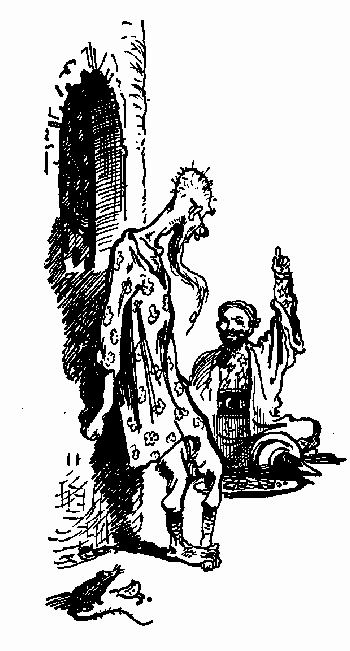
\includegraphics[scale=0.85]{14.png}
\end{figure}


Ходжа Насреддин подошел к~окну, набрал полную грудь воздуха и~вдруг завопил так, что старик, заткнув уши, шарахнулся в~сторону.

—~О~потомок нечестивых~— воскликнул~он. —~Да~где~же мне взять такую глотку, чтобы крики мои были слышны на~другом конце города!

—~Это для тебя единственный способ избегнуть рук палача,~— возразил Ходжа Насреддин.

Старику пришлось поднатужиться. Он~кричал и~вопил столь горестно, что стражники у~подножия башни прервали на~время игру и~слушали с~упоением.

После этого старик долго не~мог откашляться и~отдышаться.

—~Ох! —~говорил~он. —~Разве можно задавать такую работу моей старой гортани! Ну, доволен~ли ты~сегодня моими воплями, презренный оборванец, да~посетит тебя Азраил?!

—~Вполне доволен,~— ответил Ходжа Насреддин. —~И~вот сейчас, мудрейший Гуссейн Гуслия, ты~получишь награду за~свое усердие.

Он~вытащил кошельки, пожалованные эмиром, высыпал деньги на~поднос и~разделил на~две равные части.

Старик не~переставал ругаться и~проклинать.

—~За~что ты~ругаешь меня? —~спокойно сказал Ходжа Насреддин. —~Разве я~опозорил чем-нибудь имя Гуссейна Гуслия? Или осрамил его ученость? Вот деньги, видишь? Эмир дал их~Гуссейну Гуслия, знаменитому звездочету и~лекарю, за~то, что он~вылечил девушку из~гарема.

—~Ты~вылечил девушку? —~Старик задохнулся. —~Но~что ты~понимаешь в~болезнях, ты, невежда, плут и~голодранец!

—~Я~ничего не~понимаю в~болезнях, зато понимаю в~девушках,~— ответил Ходжа Насреддин. —~И~будет справедливо поэтому разделить эмирский подарок пополам~— тебе за~то, что ты~понимаешь, а~мне за~то, в~чем понимаю~я. Кроме того, должен сказать тебе, Гуссейн Гуслия, что я~лечил ее~не~как-нибудь, но~исследовав предварительно расположение звезд. Вчера ночью я~увидел, что звезды Сад-ад-Сууд совпали со~звездами Сад-ад-Ахбия, в~то~время как созвездие Скорпиона обратилось к~созвездию Козерога.

—~Что? —~закричал старик и~в~негодовании принялся бегать по~комнате. —~О~невежда, достойный лишь погонять ослов. Ты~не~знаешь даже того, что звезды Сад-ад-Сууд не~могут совпасть со~звездами Сад-аль-Ахбия, ибо и~те~и~другие находятся в~одном созвездии! И~как ты~мог увидеть в~это время года созвездие Скорпиона? Я~сам всю ночь смотрел на~небо, там совпадали звезды Сад-Була и~Ас-Симак, в~то~время как Аль-Джахба опускалась, ты~слышишь, невежда! Никакого Скорпиона там нет сейчас!.. Ты~перепутал, о~погонщик ослов, взявшийся не~за~свое дело, ты~принял за~Скорпиона звезды Аль-Хака, которые противостоят сейчас звездам Аль-Бутейн!..

Негодуя и~обличая Ходжу Насреддина в~невежестве, он~долго говорил об~истинном расположении звезд. Ходжа Насреддин слушал внимательно, стараясь запомнить каждое слово, дабы потом не~ошибиться, разговаривая с~эмиром в~присутствии мудрецов.

—~О~невежда, сын невежды, внук и~правнук невежды! —~продолжал старик. —~Ты~даже не~знаешь, что сейчас, в~девятнадцатое стояние луны, именуемое Аш-Шуала и~приходящееся на~знак Стрельца, человеческие судьбы определяются только звездами этого знака и~никакими другими, о~чем ясно сказано в~книге мудрейшего Шихаб-ад-дина Махмуда ибн-Караджи...

«Шихаб-ад-дина Махмуда ибн-Караджи,~— запоминал Ходжа Насреддин. —~Завтра~же в~присутствии эмира уличу бородатого мудреца в~незнании этой книги, дабы вселить в~его сердце спасительный страх перед моей ученостью...»


\chapter{}

В~доме у~ростовщика Джафара стояли двенадцать запечатанных горшков, полных золота, ему~же хотелось иметь непременно двадцать. Но~судьба, словно~бы нарочно, с~целью предостеречь неопытных и~доверчивых простаков, отметила Джафара печатью необыкновенного шельмовства: ему приходилось употреблять много усилий, чтобы завлечь в~свои сети новую жертву; горшки его наполнялись медленнее, чем он~бы хотел. «Ах, если~бы я~мог избавиться от~моего уродства! —~мечтал~он. —~Тогда люди не~разбегались~бы, завидев меня, относились~бы ко~мне с~доверием и~не~подозревали коварства в~моих речах. И~мне тогда было~бы много легче обманывать, и~мои доходы умножились~бы несравненно».

Когда по~городу разнесся слух, что новый эмирский мудрец Гуссейн Гуслия проявил необычайное искусство в~исцелении болезней, ростовщик Джафар, захватив корзину с~богатыми подарками, явился во~дворец к~Арсланбеку.

Арсланбек, заглянув в~корзину, выразил полную готовность услужить:

—~Ты~пришел как раз вовремя, почтенный Джафар. Наш повелитель пребывает сегодня в~счастливом расположении духа, я~надеюсь, что он~не~откажет тебе.

Эмир выслушал ростовщика, принял подарок, золотую шахматную доску с~белыми полями из~слоновой кости, и~приказал позвать мудреца.

—~Гуссейн Гуслия,~— сказал~он, когда Ходжа Насреддин преклонил колени перед ним. —~Вот этот человек, ростовщик Джафар,~— наш преданный раб, имеющий заслуги перед нами. Повелеваем тебе немедленно исцелить его от~горба, хромоты, бельма и~прочих уродств.

И~эмир отвернулся в~знак того, что не~желает слышать никаких возражений. Ходже Насреддину оставалось только поклониться и~выйти. Следом выполз ростовщик, влача, подобно черепахе, свой горб.

—~Пойдем~же скорее, о~мудрейший Гуссейн Гуслия! —~говорил~он, не~узнавая под фальшивой бородой Ходжу Насреддина. —~Пойдем скорее, солнце еще не~зашло, и~я~успею исцелиться до~ночи... Ты~ведь слышал~— эмир приказал тебе немедленно исцелить меня!

Ходжа Насреддин проклинал в~душе и~ростовщика, и~эмира, и~самого себя за~то, что переусердствовал в~превознесении своей мудрости. Ну~как он~выпутается теперь из~этого дела? Ростовщик дергал Ходжу Насреддина за~рукав, понуждая прибавить шагу. Улицы были пустынны, ноги Ходжи Насреддина утопали в~горячей пыли. Он~шел и~думал: «Ну~как я~теперь выпутаюсь? —~Вдруг он~остановился. —~Кажется, мне пришло время сдержать мою клятву! —~В~одно мгновение он~все рассчитал и~взвесил. —~Да, время пришло! Ростовщик, о~безжалостный истязатель бедняков, сегодня ты~будешь утоплен!» Он~отвернулся, чтобы ростовщик не~заметил блеска в~его черных глазах.

Они свернули в~переулок, где крутил по~дороге ветер, взметая пыльные смерчи. Ростовщик открыл перед Ходжой Насреддином калитку своего дома. В~глубине двора за~низеньким забором, отделявшим женскую половину. Ходжа Насреддин заметил сквозь листву какое-то движение, уловил тихий шепот и~смех. То~были жены и~наложницы, радовавшиеся приходу гостя: иных развлечений они не~знали в~своем плену. Ростовщик приостановился, грозно посмотрел~— и~все затихло... «Я~освобожу вас сегодня, прекрасные пленницы!»~— подумал Ходжа Насреддин.

Комната, в~которую привел его ростовщик, не~имела окон, а~дверь запиралась тремя замками и~еще какими-то засовами, тайна которых была известна только хозяину. Он~долго возился, звеня отмычками, прежде чем засовы упали и~дверь открылась. Именно здесь хранились горшки, здесь~же ростовщик спал на~досках, прикрывавших вход в~подземелье.

—~Разденься! —~приказал Ходжа Насреддин. Ростовщик сбросил одежду. Нагота его была неописуемо безобразна. Ходжа Насреддин закрыл дверь и~начал творить заклинания.

Тем временем во~дворе собрались многочисленные родственники Джафара. Многие из~них были должны ему и~надеялись, что сегодня на~радостях он~простит долги. Напрасно они надеялись: ростовщик слышал через закрытую дверь голоса своих должников и~злобно усмехался в~душе. «Я~скажу им~сегодня, что прощаю долги,~— думал~он,~— но~расписок я~им~не~верну, расписки останутся у~меня. И~они, успокоившись, начнут беспечную жизнь, а~я~ничего не~скажу, я~буду молчать, но~втайне все время подсчитывать. И~когда на~каждую таньга долга нарастет еще десять таньга и~сумма долга превысит стоимость домов, садов и~виноградников, принадлежащих ныне моим должникам, я~позову судью, откажусь от~своего обещания, предъявлю расписки, продам все их~имущество, оставлю их~нищими и~наполню золотом еще один горшок!» Так он~мечтал, снедаемый неутолимым корыстолюбием.

—~Встань и~оденься! —~сказал Ходжа Насреддин. —~Сейчас мы~пойдем к~водоему святого Ахмеда, и~ты~окунешься в~его священные воды. Это необходимо для твоего исцеления.

—~Водоем святого Ахмеда! —~испуганно воскликнул ростовщик. —~Я~уже тонул однажды в~его водах. Запомни, о~мудрейший Гуссейн Гуслия, что плавать я~не~умею.

—~Ты~должен на~пути к~водоему беспрерывно читать молитвы,~— сказал Ходжа Насреддин. —~И~ты~не~должен думать о~земных вещах. Кроме того, ты~возьмешь кошелек с~золотом и~каждому встречному будешь дарить золотую монету.

Ростовщик стонал и~охал, но~выполнил все в~точности. На~пути встречались ему разные люди~— ремесленники, нищие; меняясь в~лице, он~каждому дарил золотую монету. Сзади шли многочисленные родственники. Ходжа Насреддин нарочно позвал их~посмотреть, дабы избегнуть впоследствии обвинения в~преднамеренном утоплении ростовщика.

Солнце опускалось за~кровли, деревья накрыли водоем своей тенью, звенели комары. Джафар вторично разделся, подошел к~воде.

—~Здесь очень глубоко,~— сказал он~жалобно. —~Гуссейн Гуслия, ты~не~забыл: ведь я~не~умею плавать.

Родственники наблюдали в~безмолвии. Ростовщик, прикрывая ладонью свой срам и~боязливо поджимаясь, обошел вокруг водоема, выбирая место помельче.

Но~вот Джафар присел на~корточки~и, держась за~нависшие кусты, опасливо попробовал воду ногой.

—~Холодно,~— пожаловался~он; глаза его округлились.

—~Ты~слишком медлишь,~— ответил Ходжа Насреддин, стараясь не~смотреть на~ростовщика, чтобы не~допустить к~своему сердцу неправедной жалости. Но~он~вспомнил страдания бедняков, разоренных Джафаром, запекшиеся губы больного ребенка, вспомнил слезы старого Нияза; лицо Ходжи Насреддина загорелось от~гнева, он~смело и~открыто посмотрел ростовщику прямо в~глаза.

—~Ты~слишком медлишь! —~повторил~он. —~Если ты~хочешь исцелиться, то~полезай.

Ростовщик полез. Он~лез очень медленно, и~когда его ноги были по~колено в~воде, то~животом он~все еще лежал на~берегу. Наконец~— выпрямился. Глубина сразу~же у~берега была по~пояс ему. Всколыхнулись водоросли, щекоча холодными прикосновениями его тело. Зябко пошевеливая лопатками, он~шагнул вперед и~оглянулся. Сделал еще один шаг и~оглянулся. В~глазах его можно было прочесть немую мольбу. Ходжа Насреддин не~внял этой мольбе. Пожалеть ростовщика значило~бы обречь на~дальнейшие страдания тысячи бедняков.

Вода покрыла горб ростовщика, но~Ходжа Насреддин неумолимо загонял ростовщика все дальше в~глубину.

—~Еще, еще... Пусть вода коснется твоих ушей, иначе я~не~берусь исцелять. Ну, иди~же смелее, почтенный Джафар! Смелее! Шагни еще! Ну~еще немного!

—~Элп! —~вдруг сказал ростовщик и~ушел под воду с~головой.

—~Элп! —~повторил~он, показываясь через секунду на~поверхности.

—~Он~тонет! Он~тонет! —~закричали родственники. Поднялась суматоха и~толкотня, ростовщику протягивали руки, палки; одни хотели помочь ему от~чистого сердца, другие старались только для вида.

Ходжа Насреддин сразу определил, кто из~этих людей и~сколько должен. Сам он~бегал, кричал и~хлопотал больше всех:

—~Давай! Ну~давай~же руку, почтенный Джафар! Ты~слышишь, давай руку! Давай!

—~Давай! Давай! —~хором вторили родственники. Ростовщик продолжал молча нырять, показываясь на~поверхности все реже и~реже. И~здесь, в~этих священных водах, он~нашел~бы свой конец, если~бы не~прибежал откуда-то босой водонос с~пустым бурдюком за~спиной.

—~Ба! —~воскликнул~он, увидев тонущего. —~Да~ведь это ростовщик Джафар!

И, не~раздумывая, прямо как был, в~одежде, он~прыгнул в~воду, протянул руку, отрывисто крикнув:

—~На!

Ростовщик уцепился и~был благополучно вытащен. Пока~он, лежа на~берегу, приходил в~себя, водонос словоохотливо пояснял родственникам:

—~Вы~неправильно спасали его. Вы~кричали «давай», в~то~время как нужно было кричать ему «на»! Вы~знаете, конечно, что почтенный Джафар уже тонул однажды в~этом священном водоеме и~был спасен каким-то человеком, проезжавшим мимо на~сером ишаке. Этот человек применил для спасения ростовщика именно такой способ, а~я~— запомнил. Сегодня эта наука мне пригодилась...

Ходжа Насреддин слушал, кусая губы. Выходило так, что он~спас ростовщика дважды~— один раз своими руками и~второй~— руками водоноса. «Нет, я~все-таки утоплю его, хотя~бы мне пришлось для этого прожить в~Бухаре еще целый год»,~— думал~он. Тем временем ростовщик отдышался и~начал сварливо кричать:

—~О~Гуссейн Гуслия, ты~взялся исцелить меня, а~вместо этого чуть не~утопил меня! Клянусь аллахом,~— никогда больше я~не~подойду к~этому водоему ближе чем на~сто шагов! И~какой~же ты~мудрец, Гуссейн Гуслия, если не~знаешь, как нужно спасать людей из~воды; простой водонос превосходит тебя своим разумом! Подайте мой халат и~мою чалму; идем, Гуссейн Гуслия; уже темнеет, а~нам нужно завершить начатое. Водонос! —~добавил ростовщик, поднимаясь. —~Не~забудь, что срок твоему долгу истекает через неделю. Но~я~хочу наградить тебя и~поэтому прощаю тебе половину... то~есть я~хотел сказать~— четверть... нет, одну десятую часть твоего долга. Это вполне достаточная награда, ибо я~мог~бы выплыть сам, без твоей помощи.

—~О~почтенный Джафар,~— робко сказал водонос. —~Ты~не~выплыл~бы без моей помощи. Прости мне хотя~бы четверть моего долга.

—~Ага! Значит, ты~спасал меня с~корыстными целями! —~закричал ростовщик. —~Значит, в~тебе говорили не~чувства доброго мусульманина, но~одно лишь корыстолюбие! За~это, водонос, ты~подлежишь наказанию. Из~твоего долга я~ничего не~прощаю тебе!

Водонос, понурясь, отошел. Ходжа Насреддин с~жалостью посмотрел на~него, потом~— с~ненавистью и~презрением~— на~Джафара.

—~Гуссейн Гуслия, идем скорее,~— торопил ростовщик. —~О~чем ты~шепчешься там с~этим корыстолюбивым водоносом?

—~Подожди,~— ответил Ходжа Насреддин. —~Ты~забыл, что должен дарить каждому встречному золотую монету. Почему ты~ничего не~дал водоносу?

—~О, горе мне, о~разорение! —~воскликнул ростовщик. —~Этому презренному корыстолюбцу я~должен еще давать деньги! —~Он~развязал кошелек, швырнул монету. —~Пусть это будет последняя. Уже стемнело, и~мы~никого не~встретим на~обратном пути.

Но~Ходжа Насреддин не~зря шептался о~чем-то с~водоносом. Двинулись в~обратный путь~— впереди ростовщик, за~ним~— Ходжа Насреддин, сзади~— родственники. Но~не~прошли они и~пятидесяти шагов, как навстречу им~из~переулка вышел водонос,~— тот самый, которого они только что оставили на~берегу.

Ростовщик отвернулся, хотел пройти мимо. Ходжа Насреддин строгим голосом остановил его:

—~Не~забывай, Джафар: каждому встречному! В~ночном воздухе пронесся мучительный стон: это Джафар развязывал кошелек.

Получив монету, водонос исчез в~темноте. Но~через пятьдесят шагов~— опять вышел навстречу. Ростовщик побелел и~затрясся.

—~Гуссейн Гуслия,~— жалобно сказал~он. —~Посмотри, ведь это опять тот~же самый...

—~Каждому встречному,~— повторил Ходжа Насреддин.

В~тихом воздухе снова прозвучал стон. Это Джафар развязывал кошелек.

Так было всю дорогу. Водонос через каждые пятьдесят шагов попадался навстречу. Он~запыхался, дышал тяжело и~прерывисто, по~его лицу струился пот. Он~ничего не~понимал в~происходящем. Он~хватал монету и~кидался опрометью в~обход, чтобы через минуту опять выскочить откуда-нибудь из~кустов на~дорогу.

Ростовщик, спасая свои деньги, все убыстрял и~убыстрял шаги, наконец кинулся бегом. Но~разве мог он~со~своей хромотой перегнать водоноса, который, обезумев, мчался как вихрь, перемахивал через заборы; он~ухитрился выскочить навстречу ростовщику не~менее пятнадцати раз~и, наконец, перед самым домом, он~спрыгнул откуда-то с~крыши и~загородил собою калитку. Получив последнюю монету, он~в~изнеможении повалился на~землю.

Ростовщик проскочил в~калитку. За~ним вошел Ходжа Насреддин. Ростовщик швырнул к~его ногам пустой кошелек и~закричал в~бешенстве:

—~Гуссейн Гуслия, мое исцеление обходится мне слишком дорого! Я~уже потратил больше трех тысяч таньга на~подарки, на~милостыню и~на~этого проклятого водоноса!

—~Успокойся! —~ответил Ходжа Насреддин. —~Через полчаса ты~будешь вознагражден. Пусть посреди двора зажгут большой костер.

Пока слуги носили дрова и~разжигали костер. Ходжа Насреддин думал о~том, как~бы одурачить ростовщика и~взвалить на~него всю вину за~неудавшееся исцеление. Разные способы приходили ему в~голову, но~он~отвергал их~подряд, не~признавая достойными. Костер между тем разгорался, языки пламени, слегка колеблемые ветром, поднялись высоко, озарив багряным блеском листву виноградника.

—~Разденься, Джафар, и~трижды обойди вокруг костра, -сказал Ходжа Насреддин. Он~все еще не~придумал достойного способа и~выигрывал время. Лицо его было озабоченным.

Родственники наблюдали в~безмолвии. Ростовщик ходил вокруг костра, словно обезьяна на~цепи, болтая руками, свисавшими почти до~колен.

Лицо Ходжи Насреддина вдруг прояснилось. Он~облегченно вздохнул~и, откинувшись, расправил плечи.

—~Дайте мне одеяло! —~сказал он~звучным голосом. —~Джафар и~все остальные, подойдите ко~мне!

Он~выстроил родственников кольцом, а~ростовщика посадил в~середине на~землю. Потом он~обратился к~ним со~следующими словами:

—~Сейчас я~накрою Джафара этим одеялом и~прочту молитву. А~все~вы, и~Джафар в~том числе, должны, закрыв глаза, повторять эту молитву за~мной. И~когда я~сниму одеяло, Джафар будет уже исцелен. Но~я~должен предупредить вас об~одном необычайно важном условии, и~если кто-нибудь нарушит это условие, то~Джафар останется неисцеленным. Слушайте внимательно и~запоминайте.

Родственники молчали, готовые слушать и~запоминать.

—~Когда вы~будете повторять за~мною слова молитвы,~— раздельно и~громко сказал Ходжа Насреддин,~— ни~один из~вас, ни~тем более сам Джафар, не~должен думать об~обезьяне! Если кто-нибудь из~вас начнет думать о~ней или, что еще хуже, представлять ее~себе в~своем воображении~— с~хвостом, красным задом, отвратительной мордой и~желтыми клыками~— тогда, конечно, никакого исцеления не~будет и~не~может быть, ибо свершение благочестивого дела несовместимо с~мыслями о~столь гнусном существе, как обезьяна. Вы~поняли меня?

—~Поняли! —~ответили родственники.

—~Готовься, Джафар, закрой глаза! —~торжественно сказал Ходжа Насреддин, накрывая ростовщика одеялом. —~Теперь вы~закройте глаза,~— обратился он~к~родственникам. —~И~помните мое условие: не~думать об~обезьяне.

Он~произнес нараспев первые слова молитвы:

—~Мудрый аллах и~всеведущий, силою священных знаков Алиф, Лам, Мим и~Ра ниспошли исцеление ничтожному рабу твоему Джафару.

—~Мудрый аллах и~всеведущий,~— вторил разноголосый хор родственников.

И~вот на~лице одного Ходжа Насреддин заметил тревогу и~смущение; второй родственник начал кашлять, третий~— путать слова, а~четвертый~— трясти головой, точно~бы стараясь отогнать навязчивое видение. А~через минуту и~сам Джафар беспокойно заворочался под одеялом: обезьяна, отвратительная и~невыразимо гнусная, с~длинным хвостом и~желтыми клыками, неотступно стояла перед его умственным взором и~даже дразнилась, показывая ему попеременно то~язык, то~круглый красный зад, то~есть места наиболее неприличные для созерцания мусульманина.

Ходжа Насреддин продолжал громко читать молитву, и~вдруг остановился, как~бы прислушиваясь. За~ним умолкли родственники, некоторые попятились. Джафар заскрипел под одеялом зубами, ибо его обезьяна начала проделывать совсем уж~непристойные штуки.

—~Как! —~громовым голосом воскликнул Ходжа Насреддин. —~О~нечестивцы и~богохульники! Вы~нарушили мой запрет, вы~осмелились, читая молитву, думать о~том, о~чем я~запретил вам думать! —~Он~сорвал одеяло и~напустился на~ростовщика: —~Зачем ты~позвал меня! Теперь я~понимаю, что ты~не~хотел исцеляться! Ты~хотел унизить мою мудрость, тебя подучили мои враги! Но~берегись, Джафар! Завтра~же обо всем будет известно эмиру! Я~расскажу ему, что~ты, читая молитву, нарочно с~богохульными целями все время думал об~обезьяне! Берегись, Джафар, и~вы~все берегитесь: это вам не~пройдет даром, вы~знаете, какое полагается наказание за~богохульство!

А~так как за~богохульство действительно полагалось очень тяжелое наказание, то~все родственники оцепенели от~ужаса, а~ростовщик начал что-то лепетать, стараясь оправдаться. Но~Ходжа Насреддин не~слушал; он~резко повернулся и~ушел, хлопнув калиткой...

Вскоре взошла луна, залила всю Бухару мягким и~теплым светом. А~в~доме ростовщика до~поздней ночи слышались крики и~брань: там разбирались, кто первый подумал о~обезьяне...


\chapter{}

Одурачив ростовщика. Ходжа Насреддин отправился во~дворец.

Бухара засыпала, окончив дневные труды. Прохладный мрак стоял в~переулках, под мостами звучно пела вода. Пахло сырой землей, кое-где ноги Ходжи Насреддина разъезжались по~грязи: это значило, что здесь работал особенно усердный поливальщик, обильно увлажнивший дорогу, дабы порыв ночного ветра не~поднял пыли и~не~потревожил сна уставших людей во~дворах и~на~крышах. Сады, потонувшие в~темноте, дышали поверх заборов ночной, благоуханной свежестью. Далекие звезды подмигивали с~высоты Ходже Насреддину, обещали ему удачу. «Да! —~посмеивался~он. —~Мир устроен все-таки неплохо для того, кто носит на~плечах голову, а~не~пустой горшок!»

По~пути он~завернул на~базарную площадь, увидел яркие гостеприимные огни в~чайхане своего друга Али. Ходжа Насреддин обогнул чайхану, постучал в~дверь. Ему открыл сам хозяин. Они обнялись, вошли в~темную комнату. За~перегородкой слышались голоса, смех, звон посуды. Али запер дверь, зажег коптилку.

—~Все готово,~— сообщил~он. —~Я~буду ждать Гюльджан в~чайхане. Кузнец Юсуп приготовил ей~безопасное убежище. Ишак день и~ночь стоит оседланным, он~здоров, исправно кушает и~очень растолстел.

—~Спасибо, Али. Не~знаю, удастся~ли мне когда-нибудь отблагодарить тебя.

—~Удастся,~— сказал чайханщик. —~Тебе, Ходжа Насреддин, все удается, и~не~будем больше говорить о~благодарности.

Они сели, начали шептаться. Чайханщик показал мужской халат, приготовленный для Гюльджан, большую чалму, чтобы скрыть ее~косы.

Они договорились обо всем. Ходжа Насреддин уже собрался уходить, когда услышал за~стеной знакомый голос. Это был голос рябого шпиона. Ходжа Насреддин приоткрыл дверь, выглянул.

Рябой шпион, в~богатом халате, в~чалме, с~фальшивой бородкой на~лице, сидел в~кругу простолюдинов и~важно разглагольствовал:

—~Тот, кто все время выдавал себя перед вами за~Ходжу Насреддина,~— вовсе не~Ходжа Насреддин, а~просто самозванец. Настоящий Ходжа Насреддин~— это~я! Но~я~давно отрекся от~всех моих заблуждений, поняв их~гибельность и~нечестивость. И~я, настоящий, подлинный Ходжа Насреддин, советую вам всем последовать моему примеру. Я~понял наконец, что ислам~— это единственная праведная вера, понял, что наш великий, солнцеподобный эмир действительно является наместником аллаха на~земле, что доказуется его несравненной мудростью, его благочестием и~милосердием. Это говорю вам~я, подлинный и~настоящий Ходжа Насреддин!

—~Эге! —~тихонько сказал Ходжа Насреддин, подтолкнув локтем чайханщика. —~На~какие штуки они пустились, думая, что меня нет в~городе. Придется напомнить им~о~себе. Али, я~оставлю пока у~тебя свою фальшивую бороду, парчовый халат и~чалму, а~ты~дай мне какую-нибудь ветошь.

Чайханщик подал ему халат, давно уж~служивший подстилкой,~— грязный, рваный и~полный блох.

—~Ты~их~нарочно разводишь? —~спросил Ходжа Насреддин, натягивая халат. —~Ты, наверное, собираешься открыть торговлю блошиным мясом. Но~блохи съедят тебя раньше, Али.

С~этими словами он~вышел на~улицу. Чайханщик вернулся к~своим гостям, нетерпеливо ожидая, что произойдет дальше. Ждать ему пришлось недолго. Из~переулка вышел Ходжа Насреддин~— утомленной походкой человека, оставившего за~собой целый день пути. Он~поднялся в~чайхану, сел в~тени, потребовал чаю. Никто не~обращал внимания на~Ходжу Насреддина: мало~ли разных людей ходит по~бухарским дорогам?

Рябой шпион продолжал:

—~Заблуждения мои были неисчислимы, но~теперь~я. Ходжа Насреддин, раскаялся и~дал клятву быть всегда благочестивым, выполнять все предписания ислама, повиноваться эмиру, его визирям, его управителям и~стражникам. С~тех пор я~обрел покой и~блаженство и~приумножил состояние; раньше я~был презренным бродягой, а~теперь живу, как полагается жить всякому доброму мусульманину.

Какой-то погонщик с~плетью за~поясом почтительно протянул рябому шпиону пиалу с~чаем:

—~Я~приехал в~Бухару из~Коканда, о~несравненный Ходжа Насреддин. Я~много слышал о~твоей мудрости, но~я~никогда в~жизни не~думал, что мне придется встретиться с~тобой и~даже разговаривать. Теперь я~буду рассказывать всем о~встрече с~тобой и~передавать твои слова.

—~Вот, вот! —~Рябой шпион одобрительно кивнул. —~Рассказывай всем, что Ходжа Насреддин исправился, отрекся от~своих заблуждений, теперь он~благочестивый мусульманин, верный раб великого эмира. Пусть все знают об~этом.

—~У~меня есть к~тебе вопрос, о~несравненный Ходжа Насреддин,~— продолжал погонщик. —~Я~благочестивый мусульманин и~не~хочу нарушать закона даже по~неведению, между тем я~не~знаю, как нужно поступать в~тех случаях, когда купаешься в~речке и~вдруг услышишь призыв муэдзина. В~какую сторону лучше всего обратить свой взор?

Рябой шпион снисходительно усмехнулся:

—~Конечно, в~сторону Мекки... Из~темного угла донеслось:

—~В~сторону одежды. Так будет лучше всего, чтобы не~возвращаться голым домой.

Несмотря на~почтение к~рябому шпиону, все опустили головы, скрывая улыбки.

Шпион пристально посмотрел на~Ходжу Насреддина, но~в~тени не~узнал его.

—~Это кто еще там квакает из~угла? —~сказал он~высокомерно. —~Эй~ты, оборванец, ты, кажется, вздумал состязаться в~остроумии с~Ходжой Насреддином.

—~Где уж~мне, ничтожному,~— ответил Ходжа Насреддин и~скромно занялся в~своем углу чаепитием.

К~шпиону обратился какой-то крестьянин:

—~Скажи мне, о~благочестивый Ходжа Насреддин, когда мусульманину приходится участвовать в~похоронной процессии, где по~предписаниям ислама лучше всего находиться~— впереди погребальных носилок или позади?

Шпион с~важностью поднял палец, собираясь ответить, но~голос из~угла опередил его:

—~Это совершенно безразлично~— впереди или позади, лишь~бы не~на~самих носилках.

Смешливый чайханщик схватился за~пузо и~присел от~хохота; не~могли удержаться и~остальные. Этот человек в~углу не~лазил за~словом в~карман и~мог~бы, пожалуй, при случае поспорить с~Ходжой Насреддином.

Шпион, свирепея, медленно повернул голову:

—~Эй, ты, как тебя там! У~тебя, я~вижу, слишком длинный язык, как~бы тебе не~пришлось с~ним расстаться!.. Мне не~составило~бы никакого труда уничтожить его своим остроумием,~— добавил шпион, обращаясь к~людям, окружавшим его,~— но~мы~ведем сейчас благочестивую и~душеспасительную беседу, в~которой остроумие неуместно. Всему свое время, и~поэтому я~оставлю без ответа слова оборванца. Итак, я. Ходжа Насреддин, призываю вас, о~мусульмане, во~всем следовать моему примеру: уважайте мулл, повинуйтесь властям, и~благоденствие сойдет на~ваши дома. А~самое главное: не~слушайте разных подозрительных бродяг, ложно именующих себя Ходжой Насреддином, вроде того, например, бродяги, который недавно бесчинствовал в~Бухаре и~бесследно исчез, как только услышал о~прибытии в~город подлинного Ходжи Насреддина. Ловите, хватайте таких самозванцев и~предавайте их~в~руки эмирской стражи.

\begin{figure}[h]
\centering
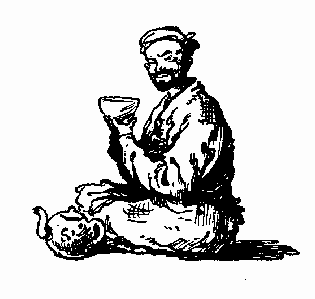
\includegraphics[scale=0.9]{15.png}
\end{figure}

—~Правильно! —~воскликнул Ходжа Насреддин, выступив из~темноты на~свет.

Все сразу узнали его, оцепенели от~неожиданности. Шпион побелел. Ходжа Насреддин вплотную подошел к~нему, а~чайханщик Али незаметно стал позади, готовый схватить шпиона в~любую минуту.

—~Значит, ты~и~есть подлинный Ходжа Насреддин? Шпион в~замешательстве оглянулся, щеки его дрожали, глаза бегали. Однако он~нашел в~себе силы ответить:

—~Да, я~и~есть подлинный, настоящий Ходжа Насреддин, все~же остальные~— самозванцы, и~ты~в~том числе!

—~Мусульмане, чего~же вы~смотрите! —~закричал Ходжа Насреддин. —~Он~сам признался! Хватайте его, держите, разве не~слышали вы~эмирского указа и~не~знаете, как надо поступать с~Ходжой Насреддином! Хватайте его, иначе вы~сами поплатитесь, как укрыватели!

Он~сорвал со~шпиона фальшивую бороду. Все в~чайхане узнали рябое ненавистное лицо с~плоским носом и~бегающими глазами.

—~Он~сам признался! —~вскричал Ходжа Насреддин, подмигнув направо. —~Хватайте Ходжу Насреддина! —~Он~подмигнул налево.

Чайханщик Али первый схватил шпиона. Тот рванулся было бежать, но~подоспели водоносы, крестьяне, ремесленники. Некоторое время ничего не~было видно, кроме поднимающихся и~опускающихся кулаков. Ходжа Насреддин старался больше всех.

—~Я~пошутил! —~кричал, стеная, шпион. —~О~мусульмане, я~пошутил, я~не~Ходжа Насреддин! Отпустите меня!

—~Врешь! —~кричал в~ответ Ходжа Насреддин, работая кулаками, подобно хорошему тестомесу. —~Ты~сам сознался, мы~слышали! О~мусульмане, мы~все здесь беспредельно преданы нашему эмиру и~должны в~точности выполнить его указ, поэтому бейте Ходжу Насреддина, о~мусульмане! Тащите его во~дворец, чтобы предать в~руки стражников! Бейте его, во~славу аллаха и~во~славу эмира!

\begin{figure}[h]
\centering
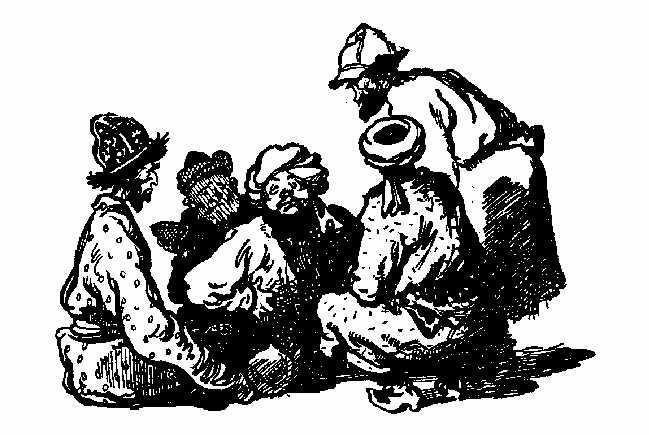
\includegraphics[width=\textwidth]{16.png}
\end{figure}

Шпиона поволокли во~дворец. Дорогой били его с~неослабевающим усердием. Ходжа Насреддин, наградив его прощальным пинком пониже спины, вернулся в~чайхану.

—~Уф! —~сказал~он, вытирая пот. —~Мы, кажется, его славно отделали! Да~и~сейчас ему достается, ты~слышишь, Али?

Издали неслись возбужденные голоса и~жалобные крики шпиона. Он~всем насолил, этот шпион, и~сегодня каждый стремился отплатить ему, прикрываясь эмир-ским указом.

Довольный и~радостный, чайханщик, усмехаясь, поглаживал пузо:

—~Это ему наука. Больше он~никогда не~придет в~мою чайхану!

Ходжа Насреддин переоделся в~задней комнате, прицепил бороду и~превратился опять в~Гуссейна Гуслия, мудреца из~Багдада.

Когда он~пришел во~дворец, то~услышал стоны, несущиеся из~караульного помещения. Он~заглянул туда.

Рябой шпион, весь опухший, избитый, измятый, лежал на~кошме, а~над ним с~фонарем в~руке стоял Арсланбек.

—~Почтенный Арсланбек, что случилось? —~невинным голосом спросил Ходжа Насреддин.

—~Очень нехорошее дело, Гуссейн Гуслия. Этот бродяга Ходжа Насреддин опять вернулся в~город и~уже успел избить нашего самого искусного шпиона, который по~моему приказанию выдавал себя всюду за~Ходжу Насреддина и~произносил благочестивые речи с~целью ослабить вредное влияние подлинного Ходжи Насреддина на~умы жителей. Но~ты~видишь, что из~этого получилось!

—~Ох, ох! —~сказал шпион, поднимая лицо, разукрашенное синяками и~кровоподтеками. —~Никогда больше не~буду я~связываться с~этим проклятым бродягой, ибо знаю, что в~следующий раз он~убьет меня. И~я~не~хочу больше служить шпионом, завтра~же я~уеду куда-нибудь подальше, где никто не~знает меня, и~займусь там честным трудом.

«Однако мои друзья постарались на~совесть! —~думал Ходжа Насреддин, разглядывая шпиона и~чувствуя даже некоторую жалость к~нему. —~Если~бы до~дворца было шагов на~двести подальше, то~вряд~ли~бы они доставили его живым. Посмотрим, пойдет~ли ему на~пользу этот урок».

На~утренней заре Ходжа Насреддин видел из~окна своей башни, как вышел из~ворот дворца рябой шпион с~маленьким узелком в~руках. Припадая то~на~правую, то~на~левую ногу, хватаясь за~грудь, за~плечи и~за~бока, поминутно присаживаясь, чтобы отдышаться, он~пересек базарную площадь, освещенную первыми прохладными лучами, и~исчез в~тени крытых рядов. На~смену темной ночи вставало утро~— чистое, прозрачное, ясное, омытое росой, пронизанное солнечным светом. Птицы щелкали, свистели и~щебетали, бабочки поднимались высоко, чтобы согреться в~первых лучах, пчела опустилась на~подоконник перед Ходжой Насреддином и~начала ползать в~поисках меда, запах которого донесся до~нее из~кувшина, стоявшего на~окне.

Всходило солнце, старинный, неизменный друг Ходжи Насреддина; каждое утро встречались они, и~каждое утро Ходжа Насреддин умел обрадоваться солнцу так, словно не~видел его целый год. Всходило солнце, как добрый, щедрый бог, равно на~всех изливающий милость, и~все в~мире, благодарно ликуя, раскрывало навстречу ему свою красоту, горело, сверкало и~сияло в~утренних лучах~— пушистые облака, изразцы минаретов, мокрые листья, вода, трава и~цветы; даже простой угрюмый булыжник, позабытый и~обделенный природой, даже~он, встречая солнце, сумел украсить себя, искрился и~блестел в~изломе, словно осыпанный алмазной пылью. И~разве мог Ходжа Насреддин в~этот час оставаться холодным перед лицом своего сияющего друга? Дерево трепетало под яркими солнечными лучами, и~Ходжа Насреддин трепетал вместе с~ним, словно сам был одет зеленой листвой; на~ближнем минарете ворковали голуби, чистили крылья, и~Ходже Насреддину хотелось почистить крыло; две бабочки порхали перед окном~— ему хотелось быть третьим в~их~легкой игре. Глаза Ходжи Насреддина сияли от~счастья, он~вспомнил рябого шпиона и~пожелал, чтобы это утро для него было утром новой жизни~— чистой и~ясной. Но~тут~же он~подумал с~огорчением, чта в~душе этого человека накопилось столько мерзости, что он~не~сможет освободиться от~нее~и, отлежавшись, возьмется опять за~старое.

Ходжа Насреддин, как это будет видно из~дальнейшего, не~ошибся в~своих предвидениях. Слишком хорошо знал он~людей, чтобы ошибаться в~них. А~как хотелось ему ошибиться, как обрадовался~бы он~духовному исцелению рябого шпиона! Но~гнилому, не~дано снова стать цветущим и~свежим, зловоние не~может превратиться в~благоухание. Ходжа Насреддин вздохнул с~огорчением.

Самой заветной мечтой его была мечта о~мире, в~котором все люди будут жить как братья, не~зная ни~алчности, ни~зависти, ни~коварства, ни~злобы, помогая друг другу в~беде и~разделяя радость каждого как общую радость. Но, мечтая о~таком счастливом мире, он~с~горечью видел, что люди живут неправильно, угнетают и~порабощают друг друга и~оскверняют души свои всяческой мерзостью. Сколько времени понадобится людям, чтобы понять наконец законы чистой и~честной жизни? А~в~том, что люди когда-нибудь поймут эти законы. Ходжа Насреддин не~сомневался нисколько. Он~твердо верил, что хороших людей на~свете гораздо больше, чем плохих; ростовщик Джафар и~рябой шпион с~их~насквозь прогнившими душами~— это лишь уродливые исключения; он~твердо верил, что от~природы человеку дается только хорошее, а~все плохое в~нем~— это чуждая накипь, привнесенная в~человеческую душу извне неправильным, несправедливо устроенным порядком жизни; он~твердо верил, что будет время, когда люди начнут перестраивать и~очищать жизнь, очищая в~этой благородной работе и~души свои от~всяческой скверны... Тому~же, что~он, Ходжа Насреддин, думал именно так, а~не~иначе, служат доказательством многочисленные истории о~нем, на~которых отпечатался чекан души его, в~том числе эта книга; и~хотя многие из~корысти, или~же низкой зависти, или по~злобе старались очернить его память, они не~достигли успеха в~своем намерении, ибо лжи никогда не~дано восторжествовать над правдой. Память о~Ходже Насреддине осталась и~впредь останется благородной и~светлой, сохраняющей, подобно алмазу, вечно и~вопреки всему свой чистый блеск! И~до~сих пор путники, останавливаясь перед скромным надгробием в~турецком Ак-Шехире, вспоминают добрым словом Ходжу Насреддина, веселого бродягу из~Бухары, и~повторяют слова поэта: «Он~отдал сердце земле, хотя и~кружился по~свету как ветер,~— как ветер, который после его смерти разнес по~вселенной благоухание цветущих роз его сердца. Прекрасна жизнь, потраченная на~то, чтобы оставить по~себе в~мире чекан души своей и~обозреть всю красоту мира! »

Впрочем, некоторые говорят, что под этим надгробием никто не~лежит, что лукавый Ходжа Насреддин нарочно поставил его~и, распустив повсюду слухи о~своей смерти, отправился дальше бродить по~свету. Так~ли было это, или не~так?.. Не~будем строить бесплодных догадок; скажем только, что от~Ходжи Насреддина можно всего ожидать!


\chapter{}

Утренние часы пролетели, на~смену им~пришел душный знойный день.

Все было готово к~побегу.

Ходжа Насреддин поднялся к~своему пленнику:

—~Срок твоего плена, мудрейший Гуссейн Гуслия, окончился. Сегодня ночью я~покидаю дворец. Я~оставлю твою комнату незапертой, но~с~тем условием, что ты~выйдешь отсюда не~раньше чем через два дня. Если~же ты~нарушишь этот срок, то~случайно можешь застать меня еще во~дворце, и~тогда, ты~сам понимаешь, мне придется обвинить тебя в~побеге и~предать палачу. Прощай, Гуссейн Гуслия, мудрец и3~Багдада, не~поминай меня лихом! Поручаю тебе открыть эмиру истину и~назвать перед ним мое имя. Слушай внимательно~— меня зовут Ходжа Насреддин!

—~О! —~воскликнул старик, отшатнувшись, и~больше ничего не~мог сказать: так поразило его это имя.

Скрипнула, закрываясь, дверь. Шаги Ходжи Насреддина затихли внизу. Старик осторожно подошел к~двери, потрогал~— она была отперта. Старик выглянул~— никого. Тогда он~поспешно захлопнул дверь и~заложил изнутри засов. «Нет! —~бормотал~он. —~Лучше я~просижу здесь еще целую неделю, только~бы не~связываться с~Ходжой Насреддином».

Вечером, когда уже загорались в~позеленевшем небе первые звезды, Ходжа Насреддин с~глиняным кувшином в~руках подошел к~стражникам, охранявшим вход в~эмирский гарем.

Стражники, не~заметив его приближения, продолжали свой разговор.

—~Вот упала еще одна звезда,~— сказал толстый ленивый стражник, поглотитель сырых яиц. —~Если они падают, как ты~говоришь, на~землю, то~почему люди никогда не~находят~их?

—~Они падают, наверное, в~море,~— ответил второй стражник.

—~Эй~вы, доблестные воины,~— вмешался Ходжа Насреддин. —~Позовите сюда главного евнуха, я~должен передать ему лекарство для больной наложницы.

Пришел главный евнух, благоговейно обеими руками принял кувшинчик, в~котором не~было ничего, кроме мела, растворенного в~простой арычной воде, выслушал подробное наставление, как нужно пользоваться этим лекарством, и~удалился.

—~О~мудрейший Гуссейн Гуслия! —~льстиво сказал толстый стражник. —~Ты~знаешь все на~свете, мудрость твоя не~имеет пределов! Скажи нам, куда падают звезды с~неба и~почему люди никогда не~находят их~на~земле?

Ходжа Насреддин не~мог удержаться, чтобы не~подшутить.

—~А~вы~разве не~знаете? —~сказал он~без тени усмешки. —~Когда звезды падают, то~рассыпаются на~мелкие серебряные монеты, а~потом нищие подбирают эти монеты. Я~даже знавал людей, которые обогатились таким образом.

Стражники переглянулись. На~их~лицах изобразилось неописуемое удивление.

Ходжа Насреддин ушел, посмеиваясь над глупыми стражниками. Он~и~подумать не~мог, как пригодится ему в~самом скором времени эта шутка.

До~полуночи он~просидел в~своей башне. Но~вот все затихло и~в~городе и~во~дворце; огни потухли. Медлить дальше было нельзя: летние ночи пролетают на~быстрых крыльях. Ходжа Насреддин сошел вниз~и, крадучись, выбирая затененные места, направился к~эмирскому гарему. «Стражники, наверное, уже уснули»,~— думал~он.

Каково~же было его огорчение, когда, приблизившись, он~услышал тихие голоса стражников.

—~Вот если~бы хоть одна звезда упала сюда! —~говорил толстый ленивый стражник. —~Мы~подобрали~бы серебро и~сразу разбогатели.

—~Знаешь, я~все-таки не~верю, чтобы звезды могли рассыпаться на~серебряные монеты,~— ответил второй стражник.

—~Но~так говорит багдадский мудрец,~— возразил первый. —~Ученость его известна всем, он, конечно, не~ошибается.

«Будьте вы~прокляты! —~мысленно восклицал Ходжа Насреддин, затаившись в~тени. —~Ах, зачем только я~сказал им~о~звездах; теперь они будут спорить до~утра! Неужели придется отложить побег?»

Над Бухарой в~недосягаемой высоте горели чистым и~тихим светом тысячи звезд: одна маленькая звезда вдруг оборвалась и~ринулась в~стремительный полет, рассекая наискось небо; вдогонку за~ней ринулась вторая звезда, оставив за~собой мгновенный, ослепительный росчерк. Была середина лета, приближалось время звездных дождей.

—~Если~бы они рассыпались на~серебряные монеты... —~начал второй стражник.

Ходжу Насреддина вдруг осенило. Он~торопливо достал из~кармана кошелек, туго набитый серебром. Ему пришлось ждать очень долго, а~звезды не~падали. Наконец одна полетела. Ходжа Насреддин бросил монету под ноги стражникам. Серебро зазвенело на~каменных плитах.

Стражники сначала оцепенели, потом приподнялись, глядя в~упор друг на~друга.

—~Ты~слышал? —~дрожащим голосом спросил первый.

—~Слышал,~— ответил второй, заикаясь. Ходжа Насреддин бросил еще монету. Она блеснула в~лунных лучах. Ленивый стражник, коротко вскрикнув, упал животом на~нее.

—~По... поймал? —~спросил немеющим языком второй.

—~По... поймал,~— ответил трясущимися губами толстяк, поднимаясь и~показывая монету.

В~небе вдруг оборвалось несколько звезд сразу. Ходжа Насреддин начал швырять серебро горстями. Тишина ночи наполнилась тонким, певучим звоном. Стражники, обезумев, побросали свои копья и~кинулись шарить по~земле.

—~Нашел! —~закричал один хриплым и~душным голосом. —~Вот она!

Второй ползал молча и~вдруг заурчал, наткнувшись на~целую россыпь монет.

Ходжа Насреддин подбросил им~еще горсть и~беспрепятственно проскользнул в~калитку.

Теперь ему было легко. Мягкие персидские ковры неслышно принимали шаги. Он~помнил все переходы. Евнухи спали...

Гюльджан встретила его влажным, горячим поцелуем и~приникла к~нему, трепеща.

—~Скорее! —~шептал~он.

Никто не~остановил~их, только евнух заворочался и~застонал во~сне. Ходжа Насреддин, пригнувшись, остановился над ним. Но~евнуху было еще рано умирать: он~почмокал губами и~опять захрапел... Слабый лунный свет пробивался сквозь разноцветные стекла.

У~самой калитки Ходжа Насреддин остановился, выглянул. Стражники, стоя на~четвереньках посреди двора, смотрели в~небо, ждали, когда упадет звезда. Ходжа Насреддин, сильно размахнувшись, бросил горсть монет; они упали где-то далеко за~деревьями. Стражники помчались туда. Они обезумели до~того, что ничего уже не~видели перед собой~и, шумно дыша, судорожно вскрикивая, ломились напрямик, через изгородь колючего кустарника, оставляя на~ветках лохмотья своих штанов и~халатов.

В~эту ночь из~гарема можно было украсть всех наложниц, а~не~только одну.

\begin{figure}[p]
\centering
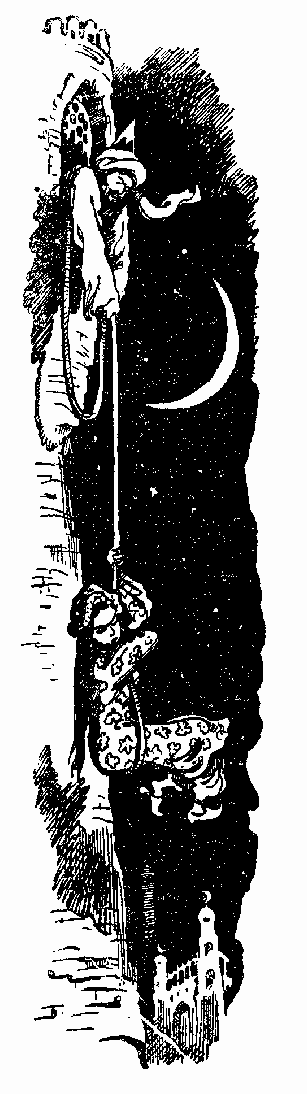
\includegraphics[scale=0.55]{17.png}
\end{figure}

—~Скорее! Скорее! —~говорил Ходжа Насреддин, увлекая за~собой девушку. Они подбежали к~башне, поднялись. Ходжа Насреддин достал из-под постели давно приготовленную веревку.

—~Здесь высоко... Я~боюсь,~— прошептала Гюльджан. Он~сердито прикрикнул на~нее, и~она покорилась.

Ходжа Насреддин обвязал ее~петлей, вынул из~окна выпиленную решетку.

Гюльджан села на~подоконник. Было очень высоко, она задрожала. «Вылезай!»~— властно сказал Ходжа Насреддин, слегка подтолкнув ее~в~спину. Она закрыла глаза, скользнула по~гладкому камню, повисла.

Она очнулась на~земле. «Беги! Беги!»~— услышала она сверху. Ходжа Насреддин высунулся до~пояса из~окна, махал руками, дергал веревку. Гюльджан поспешно отвязалась и~побежала через безлюдную площадь.

Она не~знала, что в~эту минуту весь дворец был уже объят тревогой и~смятением. Главный евнух, воспылавший после недавнего внушения тростью необычайным усердием к~эмирской службе, заглянул среди ночи в~комнату новой наложницы и~обнаружил, что постель ее~пуста. Евнух кинулся к~эмиру, разбудил его. Эмир позвал Арсланбека. Арсланбек поднял дворцовую стражу, загорелись факелы, зазвенели щиты и~копья.

Послали за~багдадским мудрецом. Эмир встретил Ходжу Насреддина крикливыми жалобами:

—~Гуссейн Гуслия, до~чего~же дошло распутство в~нашем государстве, если~мы, великий эмир, не~имеем даже в~собственном нашем дворце покоя от~этого бродяги Ходжи Насреддина! Да~слыханное~ли это дело, чтобы из~эмирского гарема украли наложницу!

—~О~великий эмир,~— осмелился вмешаться Бахтияр. —~Но~может быть, это сделал не~Ходжа Насреддин.

—~А~кто~же еще? —~закричал эмир. —~Утром нам доложили, что он~вернулся в~Бухару, а~ночью пропадает наложница, которая была его невестой! Кто еще мог это сделать, кроме Ходжи Насреддина?! Ищите его, поставьте всюду утроенные караулы,~— он, наверное, не~успел еще выбраться из~дворца! Арсланбек, запомни: твоя голова подпрыгивает на~твоих плечах!

Начались поиски. Стража обшарила все уголки во~дворце. Всюду пылали факелы, отбрасывая дрожащее зарево.

Больше всех усердствовал в~поисках сам Ходжа Насреддин. Он~приподнимал ковры, шарил палкой в~мраморных бассейнах, кричал и~суетился, заглядывая в~чайник, в~кувшины и~даже в~мышиные норы.

Вернувшись в~эмирскую опочивальню, он~доложил:

—~Великий владыка. Ходжа Насреддин уже успел покинуть дворец.

—~Гуссейн Гуслия! —~в~гневе ответил эмир. —~Твое легкомыслие удивляет нас. А~что, если он~где-нибудь спрятался? Значит, он~может проникнуть в~нашу опочивальню. Эй, стражу сюда! Стражу! —~закричал эмир, ужаснувшийся этой мысли.

За~стеной ударила пушка~— для устрашения неуловимого Ходжи Насреддина.

Эмир забился куда-то в~угол и~кричал оттуда:

—~Стражу! Стражу!

Он~не~успокоился до~тех пор, пока Арсланбек не~поставил тридцать стражников у~дверей его опочивальни и~по~десять стражников под каждым окном.

Только тогда эмир вылез из~своего угла и~сказал жалобно:

—~Как ты~думаешь, Гуссейн Гуслия, не~спрятался~ли этот бродяга где-нибудь в~нашей опочивальне?

—~Двери и~окна охраняются стражей,~— ответил Ходжа Насреддин. —~Нас в~этой комнате только двое. Откуда~же взяться здесь Ходже Насреддину?

—~Но~похищение нашей наложницы не~пройдет ему даром! —~вскричал эмир. Страх в~его душе сменился яростью, пальцы его судорожно скрючились, словно под ними он~чувствовал горло Ходжи Насреддина. —~О~Гуссейн Гуслия! —~продолжал эмир. —~Нет предела нашему гневу и~нашему возмущению! Ведь мы~так и~не~успели ни~разу войти к~ней; мысль об~этом переполняет скорбью наше царственное сердце! А~виноваты во~всем, о~Гуссейн Гуслия, твои звезды; если~бы мы~могли, отрубили~бы всем звездам головы за~подобные злонамеренные поступки! Но~на~этот раз Ходжа Насреддин не~ускользнет безнаказанно! Мы~уже отдали приказание Арсланбеку! Тебе, Гуссейн Гуслия, мы~также поручаем приложить все усердие к~поимке бродяги! Запомни, что от~успеха в~этом деле зависит твое назначение на~должность главного евнуха. Завтра ты~должен покинуть дворец, Гуссейн Гуслия, и~не~возвращаться обратно без Ходжи Насреддина.

Щуря лукавые, ясные глаза. Ходжа Насреддин склонился перед эмиром до~земли.


\chapter{}

До~утра Ходжа Насреддин рассказывал эмиру о~своих планах поимки Ходжи Насреддина. Планы эти были весьма хитроумны, эмир остался доволен.

Утром, получив на~расходы кошелек золота. Ходжа Насреддин в~последний раз поднялся в~башню, уложил в~кожаный пояс деньги и~огляделся со~вздохом: ему вдруг стало жаль покидать свое жилище,~— столько одиноких бессонных ночей провел он~здесь и~столько передумал; он~оставлял в~этих угрюмых стенах частицу своей души.

Он~захлопнул за~собой дверь, легко сбежал по~каменной крутой лестнице~— навстречу свободе. Опять весь мир был открыт перед ним. Дороги, перевалы и~горные тропы звали его в~дальний путь, зеленые леса обещали ему приют в~тени на~мягких листьях, реки ждали его, чтобы напоить студеной водой, птицы приготовили на~радость ему самые лучшие песни,~— он~слишком долго пробыл в~своей позолоченной клетке, веселый бродяга Ходжа Насреддин, и~мир соскучился без него.

Но~у~самых ворот прямо в~сердце ему был нанесен страшный удар.

Он~остановился~и, побледнев, прижался к~стене. В~открытые ворота под охраной многочисленных стражников входили вереницей с~опущенными головами и~связанными руками его друзья; он~увидел старого горшечника Нияза, чайханщика Али, кузнеца Юсупа и~многих других; все, с~кем он~когда-либо встречался, говорил, у~кого просил воды напиться или брал клочок сена для ишака,~— все были здесь!.. Печальное шествие замыкал Арсланбек.

Не~скоро опомнился Ходжа Насреддин, а~когда опомнился~— ворота уже закрылись и~во~дворе никого не~было: всех увели в~подземелье. Ходжа Насреддин кинулся, искать Арсланбека.

—~Что случилось, почтенный Арсланбек? Кто эти люди? Какое преступление совершили они?

—~Эти люди~— укрыватели и~сообщники проклятого Ходжи Насреддина! —~ответил с~торжеством Арсланбек. —~Мои шпионы выследили~их, и~сегодня~же они всенародно будут преданы жестокой казни, если не~выдадут Ходжу Насреддина. Но~ты~бледен, Гуссейн Гуслия! Ты~сильно расстроен!..

—~Еще~бы! —~ответил Ходжа Насреддин. —~Значит, награда уплывает из~моих рук в~твои!

Ходже Насреддину пришлось остаться во~дворце. Да~разве мог он~поступить иначе, если невинным людям грозила смерть?

В~полдень на~площади выстроилось войско, оцепив тройным кольцом судейский помост. Народ, оповещенный глашатаями о~предстоящих казнях, ждал, безмолвствуя. Раскаленное небо дышало палящим зноем.

Открыли ворота дворца, и~в~обычном порядке выбежали сначала глашатаи, за~ними~— стража, вышли музыканты, слоны, свита, и, наконец, выплыли из~ворот эмирские носилки. Народ распростерся ниц. Носилки поднялись на~помост.

Эмир занял свое место на~троне. Из~ворот дворца вывели осужденных. Толпа встретила их~появление гулом. Родственники и~друзья осужденных стояли в~первых рядах, чтобы лучше видеть.

Палачи хлопотали, готовили топоры, колья, веревки. Сегодня у~палачей был трудный день: им~предстояло умертвить подряд шестьдесят человек.

Старый Нияз был первым в~этой роковой очереди. Палачи держали его под руки, справа от~него была виселица, слева~— плаха, а~прямо перед ним торчал из~земли заостренный кол.

Великий визирь Бахтияр громко и~торжественно объявил:

—~Во~имя аллаха милостивого и~милосердного! Повелитель Бухары и~солнце вселенной, эмир бухарский, взвесив на~весах справедливости прегрешения, которые совершили шестьдесят его подданных по~укрывательству богохульника, возмутителя спокойствия, сеятеля раздоров и~совершителя непристойных дел Ходжи Насреддина, постановил следующее: горшечника Нияза, как главного укрывателя, у~которого означенный бродяга, именуемый Ходжой Насреддином, долгое время скрывался,~— лишить жизни через отделение его головы от~его туловища. Что~же касается прочих преступников, то~первым наказанием для них будет лицезрение казни, которая совершится над Ниязом, дабы они трепетали, ожидая для себя еще худшей участи. О~способе казни каждого из~них будет возглашено особо...

На~площади стояла такая тишина, что каждое слово Бахтияра отчетливо слышалось в~задних рядах.

—~И~да~будет всем ведомо,~— продолжал~он, возвысив голос,~— что и~впредь со~всяким укрывателем Ходжи Насреддина будет поступлено так~же, и~ни~один не~уйдет от~руки палача. Если~же кто-либо из~осужденных укажет местопребывание этого вора и~бездельника, тот не~только будет освобожден от~казни, не~только станет обладателем эмирской награды и~небесного благословения, но~и~освободит от~наказания всех прочих. Горшечник Нияз, ты~можешь избавить себя и~других от~казни, если откроешь местопребывание Ходжи Насреддина.

Нияз долго молчал, не~поднимая головы. Бахтияр повторил свой вопрос.

Нияз ответил:

—~Нет, я~не~могу указать его местопребывание. Палачи потащили старика к~плахе. Кто-то крикнул в~толпе. Старик стал на~колени~и, вытянув шею, положил на~плаху седую голову.

В~эту минуту Ходжа Насреддин, растолкав придворных, выступил вперед и~стал перед эмиром.

—~О~повелитель! —~сказал он~громко, так, чтобы слышал народ. —~Прикажи остановить казнь, я~сейчас поймаю Ходжу Насреддина!

Эмир воззрился на~него с~удивлением. Народ на~площади зашевелился. Палач, повинуясь знаку эмира, опустил к~ногам свой топор.

—~О~владыка! —~громко сказал Ходжа Насреддин. —~Будет~ли справедливо, чтобы этих мелких укрывателей предали казни, в~то~время как останется живым самый главный укрыватель, у~которого Ходжа Насреддин жил все последнее время и~живет сейчас, который поил, кормил, награждал его и~проявлял о~нем всяческую заботу?

—~Ты~прав,~— сказал эмир важно. —~Если есть такой укрыватель, то~по~справедливости ему должно отрубить голову первому. Но~укажи нам этого укрывателя, Гуссейн Гуслия.

По~толпе прошел сдержанный ропот; передние передавали задним слова эмира.

—~Но~если великий эмир не~захочет казнить этого главного укрывателя, если великий эмир оставит его живым, то~справедливо~ли будет тогда предавать казни малых укрывателей? —~спросил Ходжа Насреддин.

Эмир ответил, удивляясь все больше:

—~Если мы~не~пожелаем казнить главного укрывателя, то, конечно, откажемся от~казни мелких укрывателей. Но~одно непонятно нам, Гуссейн Гуслия:

какие причины могут заставить нас воздержаться от~казни главного укрывателя? Где он? Укажи его нам, и~мы~немедленно отделим его голову от~его туловища.

Ходжа Насреддин обратился к~народу:

—~Вы~слышали слова эмира. Повелитель Бухары сказал, что если он~откажется казнить главного укрывателя, которого я~сейчас назову, тогда все эти малые укрыватели, стоящие сейчас у~плахи, будут освобождены и~отпущены к~своим семьям. Так~ли я~сказал, о~повелитель?

—~Ты~правильно сказал, Гуссейн Гуслия,~— подтвердил эмир. —~Даем в~этом наше слово. Но~укажи нам скорее главного укрывателя.

—~Вы~слышите? —~сказал Ходжа Насреддин, повернувшись к~народу. —~Эмир дает слово!

Он~глубоко вздохнул. Он~чувствовал на~себе тысячи глаз.

—~Самый главный укрыватель...

Он~запнулся, обвел глазами площадь; многие заметили скорбь и~смертную тоску на~его лице. Он~прощался со~своим любимым миром, с~людьми и~солнцем.

—~Скорее! —~нетерпеливо воскликнул эмир. —~Говори скорее, Гуссейн Гуслия!

Ходжа Насреддин сказал твердым, звонким голосом:

\begin{figure}[p]
\centering
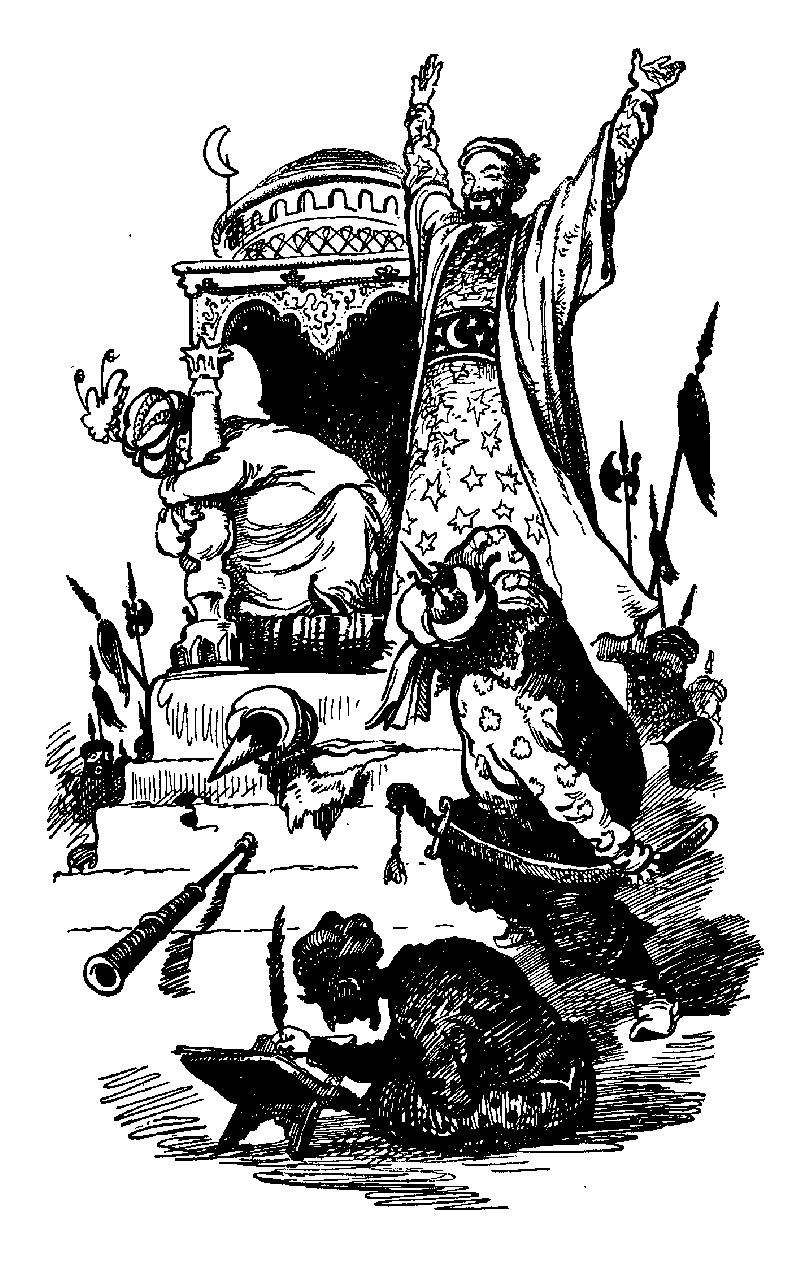
\includegraphics[width=\textwidth]{18.png}
\end{figure}

—~Самый главный укрыватель~— это~ты, эмир!

Резким движением он~сбросил свою чалму, сорвал фальшивую бороду.

Толпа ахнула, замерла. Эмир, выпучив глаза, беззвучно шевелил губами. Придворные окаменели.

Тишина продолжалась недолго.

—~Ходжа Насреддин! Ходжа Насреддин! —~закричали в~толпе.

—~Ходжа Насреддин! —~зашептались придворные.

—~Ходжа Насреддин! —~воскликнул Арсланбек. Наконец опомнился и~сам повелитель. Губы его невнятно вымолвили:

—~Ходжа Насреддин!

—~Да, это~я! Ну~что~же, эмир, прикажи отрубить себе голову~— как самому главному укрывателю! Я~жил у~тебя во~дворце, делил с~тобою пищу, получал от~тебя награды, я~был твоим главным и~ближайшим советником во~всех делах. Ты~— укрыватель, эмир, прикажи отрубить себе голову!

Ходжу Насреддина схватили. Он~не~сопротивлялся, он~кричал:

—~Эмир обещал освободить осужденных! Вы~слышали слово эмира.

Народ начал гудеть, волноваться. Тройная цепь стражников с~трудом сдерживала напор толпы. Все громче слышались возгласы:

—~Освободите осужденных!

—~Эмир дал слово!..

—~Освободите!..

Гул в~толпе нарастал и~ширился. Цепи стражников подавались назад, теснимые народом. Бахтияр наклонился к~эмиру:

—~О, повелитель, их~нужно освободить, иначе народ взбунтуется.

Эмир кивнул.

—~Эмир держит свое слово! —~закричал Бахтияр. Стражники расступились. Осужденные сразу исчезли в~толпе.

Ходжу Насреддина повели во~дворец. Многие в~толпе плакали, кричали ему вслед:

—~Прощай, Ходжа Насреддин! Прощай, наш любимый, благородный Ходжа Насреддин, ты~будешь всегда бессмертен в~наших сердцах.

Он~шел с~высоко поднятой головой, на~его лице было бесстрашие. Перед воротами он~обернулся, махнул на~прощание рукой. Толпа ответила ему мощным рокотом.

Эмир торопливо залез в~свои носилки. Дворцовое шествие тронулось в~обратный путь.


\chapter{}

Собрался диван~— судить Ходжу Насреддина.

Когда он~вошел, связанный по~рукам и~ногам, охраняемый стражниками,~— придворные потупились. Им~было стыдно смотреть друг на~друга. Мудрецы морщились, оглаживая бороды, эмир, отвернувшись, вздыхал и~покашливал.

А~Ходжа Насреддин смотрел прямым, ясным взглядом; если~бы не~его закрученные за~спину руки, то~можно было~бы подумать, что преступник не~он, а~все эти люди, сидящие перед ним.

На~суд вместе с~другими придворными явился и~подлинный Гуссейн Гуслия, багдадский мудрец, освобожденный наконец из~своего заточения. Ходжа Насреддин дружески подмигнул ему, багдадский мудрец подскочил на~подушках и~зашипел от~ярости.

Суд продолжался недолго. Ходжу Насреддина приговорили к~смерти. Оставалось избрать способ казни.

—~О~великий владыка! —~сказал Арсланбек. —~Мое мнение, что этого преступника необходимо посадить на~кол, дабы он~окончил жизнь свою в~жесточайших мучениях.

Ходжа Насреддин даже бровью не~дрогнул; он~стоял и~безмятежно улыбался, подставив лицо солнечному лучу, падавшему в~зал через верхнее открытое окно.

—~Нет! —~решительно сказал эмир. —~Султан турецкий уже сажал на~кол этого богохульника, но~он, по-видимому, знает средство переносить без вреда для себя подобный способ казни, иначе он~не~ушел~бы живым из~рук султана.

Бахтияр посоветовал отрубить Ходже Насреддину голову.

—~Правда, это один из~наилегчайших видов смерти,~— добавил~он,~— но~зато самый верный.

—~Нет! —~сказал эмир. —~Калиф багдадский рубил ему голову, а~он~все-таки жив.

Поочередно поднимались сановники, предлагали повесить Ходжу Насреддина, содрать с~него кожу. Эмир отверг все эти советы, потому что, наблюдая тайком за~Ходжой Насреддином, не~замечал признаков страха на~его лице, что было в~глазах эмира явным доказательством недействительности предлагаемых способов.

Придворные замолчали в~смущении. Эмир начал гневаться.

Тогда поднялся багдадский мудрец. Впервые он~говорил перед лицом эмира, поэтому тщательно обдумал свой совет, дабы отличиться мудростью от~всех прочих.

—~О~великий повелитель вселенной! Если этот преступник уходил до~сих пор невредимым от~всевозможных способов казни, то~не~является~ли это прямым свидетельством того, что ему помогает нечистая сила, тот самый дух тьмы, имя которого непристойно называть здесь, перед лицом эмира.

При этих словах мудрец подул себе на~плечи, вслед за~ним подули все остальные, кроме Ходжи Насреддина.

—~Рассудив и~взвесив все, касающееся этого преступника,~— продолжал мудрец,~— наш великий эмир отверг предложенные способы умерщвления Ходжи Насреддина, опасаясь, что нечистая сила вновь поможет преступнику ускользнуть от~справедливой кары. Но~существует еще один способ казни, которому названный преступник Ходжа Насреддин ни~разу не~подвергался, а~именно~— утопление!

Багдадский мудрец, высоко вскинув голову, с~торжеством посмотрел на~присутствующих.

Ходжа Насреддин встрепенулся.

Эмир заметил его движение. «Ага! Так вот в~чем была его тайна!»

Ходжа Насреддин думал в~это время: «Очень хорошо, что они заговорили о~нечистой силе; значит, надежда еще не~потеряна для меня!»

—~Известно мне из~рассказов и~книг,~— продолжал между тем мудрец,~— что в~Бухаре имеется священный водоем, именуемый водоемом шейха Ахмеда. Понятно, что нечистая сила не~осмеливается приближаться к~этому водоему, почему и~надлежит, о~повелитель, погрузить преступника на~длительный срок с~головой в~священные воды, после чего он~умрет.

—~Вот совет мудреца, достойный награды! —~воскликнул эмир.

Ходжа Насреддин укоризненно сказал багдадскому мудрецу:

—~О~Гуссейн Гуслия, так~ли я~обращался с~тобой, когда ты~был в~моей власти? Вот и~надейся после этого на~людскую благодарность!

Было решено после захода солнца всенародно утопить Ходжу Насреддина в~священном водоеме шейха Ахмеда. А~чтобы по~дороге Ходжа Насреддин не~смог убежать, решили доставить его из~дворца к~водоему в~кожаном мешке и~в~этом~же мешке утопить.

...Целый день у~водоема стучали топоры: плотники возводили помост, но~что могли они сделать, если над каждым из~них стоял стражник? Они работали молча, с~угрюмыми, ожесточенными лицами; закончив, они отказались получить скудную плату и~ушли, глядя в~землю.

Помост и~весь берег вокруг устлали коврами. Противоположный берег предназначался для народа.

Шпионы доносили, что город волнуется. Поэтому Арсланбек согнал к~водоему великое множество войска, поставил пушки. Опасаясь, как~бы народ по~дороге не~отбил Ходжу Насреддина, Арсланбек приказал приготовить четыре мешка, набитых тряпьем:

эти фальшивые мешки он~намеревался отправить к~водоему открыто, по~людным улицам, а~мешок с~Ходжой Насреддином, наоборот,~— самыми глухими переулками. Хитрость свою он~простер еще дальше: к~фальшивым мешкам он~приставил по~восемь стражников, а~к~мешку с~Ходжой Насреддином только троих.

—~Я~пришлю к~вам от~водоема гонца,~— сказал стражникам Арсланбек. —~Четыре фальшивых мешка вы~должны вынести сразу, один за~другим, а~пятый мешок, с~преступником,~— немного погодя и~незаметно, когда все любопытные, толпящиеся у~ворот, устремятся за~фальшивыми мешками. Хорошо~ли поняли вы~меня? Помните, что отвечать придется вам головой.

Вечером на~площади ударили барабаны, возвещая об~окончании базара. К~водоему со~всех сторон потянулись толпы народа. Вскоре прибыл эмир со~свитой. На~помосте и~вокруг него зажгли факелы. Пламя шипело и~гнулось от~ветра, на~воде дрожали багровые отблески. Противоположный берег тонул в~темноте; с~помоста, озаренного огнями, не~видно было толпы, но~ясно слышалось, как ворочается, движется и~дышит она, сливая свой смутный тревожный гул с~порывами ночного ветра.

Бахтияр громким голосом прочитал в~темноту эмир-ский указ о~предании смерти Ходжи Насреддина. В~это время и~ветер улегся,~— была тишина, такая, что у~светлейшего эмира поползли мурашки по~спине. Опять вздохнул ветер, вместе с~ним вздохнула тысячами грудей толпа.

—~Арсланбек! —~сказал эмир, и~голос его дрогнул. —~Почему ты~медлишь?

—~Я~уже отправил гонца, о~повелитель. Вдруг в~темноте послышались крики, лязг оружия; где-то началась свалка. Эмир подпрыгнул, озираясь. Через минуту в~освещенный круг перед помостом вошли восемь стражников без мешка.

—~Где~же преступник? —~вскричал эмир,~— Его отняли у~стражников, он~ускользнул! Арсланбек, ты~видишь!

—~О~повелитель! —~ответил Арсланбек. —~Твой ничтожный раб предусмотрел все; в~этом мешке были старые тряпки.

В~другой стороне опять послышался шум свалки. Арсланбек поспешил успокоить эмира:

—~Пусть отнимают, о~повелитель! В~этом мешке тоже ничего нет, кроме тряпок.

...Первый мешок отбил у~стражников чайханщик Али со~своими друзьями, второй отбили кузнецы, возглавляемые Юсупом. Вскоре гончары отбили третий мешок, но~и~в, нем оказались тряпки. Четвертый мешок пропустили к~помосту свободно. Стражники при свете факелов на~глазах у~всей толпы подняли мешок над водой и~вытряхнули; посыпались тряпки.

Толпа замерла в~полном недоумении. Этого и~добивался многоопытный Арсланбек, понимавший, что недоумение влечет за~собою бездействие.

Настало время пятому мешку. Между тем стражники, которым он~был поручен, задержались где-то и~до~сих пор не~доставили его к~водоему.


\chapter{}

Когда стражники вывели Ходжу Насреддина из~подземелья, он~сказал:

—~Значит, вы~потащите меня на~собственных спинах? Жалею, что здесь нет моего ишака, он~бы лопнул от~смеха.

—~Молчи! Скоро тебе придется заплакать! —~злобно ответили стражники. Они не~могли простить Ходже Насреддину, что он~предался в~руки эмира помимо стражи.

Распялив тесный мешок, они начали запихивать в~него Ходжу Насреддина.

—~О~слуги шайтана! —~кричал Ходжа Насреддин, сложенный втрое. —~Неужели вы~не~могли выбрать мешок попросторнее!

—~Ничего! —~говорили стражники, пыхтя и~обливаясь потом. —~Тебе недолго придется терпеть. Не~растопыривайся~же, о~сын греха, иначе мы~вдавим твои колени в~твой живот!

Поднялся шум, сбежалась дворцовая челядь. Наконец после долгих трудов стражники запихали Ходжу Насреддина в~мешок и~завязали веревкой. В~мешке было тесно, темно и~вонюче. Душа Насреддина окуталась черным туманом; казалось, спасения для него теперь нет. Он~взывал к~судьбе и~всемогущему случаю:

«О~ты, судьба, ставшая для меня матерью, о~ты, всемогущий случай, оберегавший меня до~сих пор, подобно отцу,~— где вы~сейчас, почему не~поспешите на~помощь к~Ходже Насреддину? О~судьба, о~всемогущий случай!»

А~стражники уже прошли половину пути; они несли мешок, меняясь через каждые двести шагов; по~этим коротким остановкам Ходжа Насреддин вел печальный счет~— сколько пройдено и~сколько осталось.

Он~хорошо понимал, что судьба и~случай никогда не~приходят на~помощь к~тому, кто заменяет дело жалобами и~призывами. Дорогу осилит идущий; пусть в~пути ослабнут и~подогнутся его ноги~— он~должен ползти на~руках и~коленях, и~тогда обязательно ночью вдали увидит он~яркое пламя костров~и, приблизившись, увидит купеческий караван, остановившийся на~отдых, и~караван этот непременно окажется попутным, и~найдется свободный верблюд, на~котором путник доедет туда, куда нужно... Сидящий~же на~дороге и~предающийся отчаянию~— сколь~бы ни~плакал он~и~ни~жаловался~— не~возбудит сочувствия в~бездушных камнях; он~умрет от~жажды в~пустыне, труп его станет добычей смрадных гиен, кости его занесет горячий песок. Сколько людей умерли преждевременно, и~только потому, что недостаточно сильно хотели жить! Такую смерть Ходжа Насреддин считал позорной для человека.

«Нет! —~сказал он~себе~и, стиснув зубы, яростно повторил: —~Нет! Я~не~умру сегодня! Я~не~хочу умирать!»

Но~что он~мог сделать, сложенный втрое и~засунутый в~тесный мешок, где нельзя было даже пошевелиться: колени и~локти как будто прилипли к~туловищу. Свободным у~Ходжи Насреддина оставался только язык.

—~О~доблестные воины,~— сказал он~из~мешка. —~Остановитесь на~минутку, я~хочу прочесть перед смертью молитву, дабы всемилостивый аллах принял мою душу в~светлые селения свои.

Стражники опустили мешок на~землю:

—~Читай. Но~из~мешка мы~тебя не~выпустим. Читай свою молитву в~мешке.

—~А~где мы~находимся? —~спросил Ходжа Насреддин. —~Я~это затем спрашиваю, чтобы вы~обратили меня лицом к~ближайшей мечети.

—~Мы~находимся близ Каршинских ворот. Здесь кругом мечети, в~какую~бы сторону мы~тебя не~обратили лицом. Читай~же скорее свою молитву. Мы~не~можем долго задерживаться.

—~Спасибо, о~благочестивые воины,~— печальным голосом ответил из~мешка Ходжа Насреддин.

На~что он~рассчитывал? Он~и~сам не~знал. «Я~выгадаю несколько минут. А~там посмотрим. Может быть, что-нибудь подвернется...»

Он~начал громко молиться, прислушиваясь в~то~же время к~разговорам стражников.

—~И~как мы~не~сообразили сразу, что новый звездочет~— это и~есть Ходжа Насреддин? —~сокрушались стражники. —~Если~бы мы~узнали и~поймали его, то~получили~бы от~эмира большую награду!

Мысли стражников текли в~обычном направлении, ибо алчность составляла самую сущность их~жизни.

Этим и~воспользовался Ходжа Насреддин. «Попробую сделать так, чтобы они ушли куда-нибудь от~мешка, хотя~бы на~самый короткий срок... Может быть, мне удастся порвать веревку, может быть, кто-нибудь пройдет по~дороге и~освободит меня».

—~Скорей кончай молитву! —~говорили стражники, толкая мешок ногами. —~Слышишь, ты! Нам некогда ждать!

—~Одну минуту, доблестные воины! У~меня осталась последняя просьба к~аллаху. О~всемогущий, всемилостивый аллах, сделай так, чтобы тот человек, который найдет закопанные мнрю десять тысяч таньга, выделил~бы из~них одну тысячу, и~отнес в~мечеть, и~отдал мулле, поручив ему молиться за~меня в~течение целого года...

Услышав о~десяти тысячах таньга, стражники притихли. Хотя Ходжа Насреддин ничего не~видел из~своего мешка, но~точно знал, какие сейчас у~стражников лица, как они переглядываются и~толкают друг друга локтями.

—~Несите меня дальше,~— сказал он~кротким голосом. —~Предаю дух мой в~руки аллаха. Стражники медлили.

—~Мы~еще немного отдохнем,~— вкрадчиво сказал один из~них. —~О~Ходжа Насреддин, не~думай, что мы~бессердечные, нехорошие люди. Только служба заставляет нас поступать с~тобою столь жестоко; если~бы мы~могли прожить с~нашими семьями без эмирского жалованья, тогда~мы, конечно, немедленно выпустили~бы тебя на~волю...

—~Что ты~говоришь! —~испуганно прошептал второй. —~Если мы~его выпустим, то~эмир снимет нам головы.

—~Молчи! —~зашипел первый. —~Нам~бы только получить деньги.

Ходжа Насреддин не~слышал шепота, но~знал, что стражники шепчутся, и~знал, о~чем они шепчутся.

—~Я~не~имею зла на~вас, о~воины,~— сказал он~с~благочестивым вздохом. —~Я~сам чересчур грешен для того, чтобы осуждать других. Если аллах дарует мне прощение на~том свете, обещаю вам помолиться за~вас перед его троном. Вы~говорите, что если~бы не~эмирское жалованье, то~вы~бы меня выпустили? Подумайте над своими словами! Ведь этим вы~нарушили~бы волю эмира~и, следовательно, совершили~бы тяжкий грех. Нет! Я~не~хочу, чтобы вы~из-за меня отягощали грехом свои души; поднимайте мешок, несите меня к~водоему, пусть свершится воля эмира и~воля аллаха!..

Стражники в~растерянности переглядывались, проклиная благочестивое раскаяние, которое вдруг~— и~совсем, по~их~мнению, не~вовремя~— овладело Ходжой Насреддином.

В~разговор вступил третий стражник: до~сих пор он~молчал, придумывая хитрость.

—~Сколь тяжко видеть человека, который перед смертью начал раскаиваться в~своих грехах и~заблуждениях,~— сказал~он, подмигивая товарищам. —~Нет, я~не~таков! Я~уже давно раскаялся и~давно веду благочестивый образ жизни. Но~благочестие на~словах, не~сопровождаемое угодными аллаху делами,~— мертво,~— продолжал стражник, в~то~время как товарищи его зажимали рты ладонями, чтобы не~расхохотаться, ибо он~был известен как неисправимый игрок в~кости и~распутник. —~Вот~я, например, сопровождаю свою благочестивую жизнь праведным и~благочестивым делом, а~именно: я~строю в~моем родном селении большую мечеть и~ради этого отказываю даже в~пище себе и~своей семье.

Один из~стражников не~выдержал~и, давясь от~смеха, ушел в~темноту.

—~Я~откладываю каждый грош,~— продолжал благочестивый стражник,~— и~все-таки мечеть воздвигается слишком медленно, что переполняет скорбью мое сердце. На~днях я~продал корову. Пусть мне придется продать последние сапоги~— я~согласен ходить босиком, лишь~бы завершить начатое.

Ходжа Насреддин всхлипнул в~мешке. Стражники переглянулись. Дело у~них шло на~лад. Они локтями торопили своего догадливого товарища.

—~О, если~бы мне повстречался такой человек, который согласился~бы пожертвовать восемь или десять тысяч таньга на~окончание этой мечети! —~воскликнул~он. —~Я~бы поклялся перед ним, что в~течение пяти и~даже десяти лет имя его ежедневно возносилось~бы, окутанное благоуханным дымом молитвы, из-под сводов этой мечети к~трону аллаха! Первый стражник сказал:

—~О~мой благочестивый товарищ! У~меня нет десяти тысяч таньга, но~может быть, ты~согласишься принять мои последние сбережения~— пятьсот таньга. Не~отвергай моего скромного дара, мне тоже хочется принять участие в~этом праведном деле.

—~И~мне,~— сказал второй, заикаясь и~дрожа от~внутреннего смеха. —~У~меня есть триста таньга...

—~О~праведник, о~благочестивей! —~воскликнул Ходжа Насреддин, всхлипывая. —~Как я~жалею, что не~могу приложить к~своим губам край твоего халата! Я~великий грешник, но~будь милостив ко~мне и~не~отвергни моего дара. У~меня есть десять тысяч таньга. Когда~я, совершив богохульный обман, был приближен к~эмиру, то~часто получал от~него в~подарок кошельки с~золотом и~серебром; накопив десять тысяч таньга, я~решил спрятать~их, с~тем чтобы, свершая бегство, захватить по~дороге. А~так как я~решил бежать через Каршинские ворота, то~и~закопал эти деньги на~Каршинском кладбище под одним из~старых надгробий.

—~На~Каршинском кладбище! —~воскликнули стражники. —~Значит, они где-то здесь, рядом!

—~Да! Сейчас мы~находимся на~северном конце кладбища, и~если пройти...

—~Мы~находимся на~восточном конце! Где, где они спрятаны, твои деньги?

—~Они спрятаны на~западном конце кладбища,~— сказал Ходжа Насреддин. —~Но~сначала поклянись мне, о~благочестивый стражник, что мое имя действительно будет поминаться в~мечети ежедневно в~течение десяти лет.

—~Клянусь! —~сказал стражник, дрожа от~нетерпения. —~Клянусь тебе именем аллаха и~пророка его Магомета! Ну, говори скорее, где закопаны твои деньги?

Ходжа Насреддин медлил. «А~что, если они решат отнести меня сначала к~водоему, отложив на~завтра поиски денег? —~думал~он. —~Нет, этого не~случится. Во-первых, они обуяны алчностью и~нетерпением, во-вторых, они побоятся, что кто-нибудь может опередить~их, втретьих, они не~доверяют друг другу. Какое~же указать им~место, чтобы они подольше копались?»

Стражники ждали, склонившись над мешком. Ходжа Насреддин слышал их~отяжелевшее дыхание, как будто они только что прибежали откуда-то издалека.

—~На~западном конце кладбища есть три старых надгробия, расположенные треугольником,~— сказал Ходжа Насреддин. —~Под каждым из~них я~закопал по~три тысячи триста тридцать три таньга с~одной третью...

—~Расположенные треугольником,~— хором повторяли стражники, уподобляясь послушным ученикам, повторяющим за~своим учителем слова корана. —~По~три тысячи триста тридцать три таньга с~одной третью...

Они сговорились, что двое пойдут за~деньгами, а~третий останется караулить. Это могло~бы повергнуть Ходжу Насреддина в~уныние, если~бы он~не~обладал способностью наперед угадывать человеческие поступки: он~точно знал, что третий стражник недолго усидит около мешка. Предвидения оправдались: оставшись один, стражник начал беспокойно вздыхать, кашлять, ходить взад-вперед по~дороге, звеня оружием. По~этим звукам Ходжа Насреддин угадывал все его мысли: стражника грызла тревога за~свои три тысячи триста тридцать три таньга с~одной третью. Ходжа Насреддин терпеливо ждал.

—~Как долго они там возятся,~— сказал стражник.

—~Они, наверное, прячут деньги куда-нибудь в~другое место, а~завтра вы~все трое придете за~ними,~— ответил Ходжа Насреддин.

Это был меткий удар. Стражник шумно засопел, потом начал притворно зевать.

—~Как хочется мне перед смертью послушать какую-нибудь душеспасительную историю,~— сказал из~мешка Ходжа Насреддин. —~Может быть, ты~вспомнишь и~расскажешь мне, о~добрый стражник.

—~Нет! —~сердито ответил стражник. —~Я~не~знаю душеспасительных историй... К~тому~же, я~устал, пойду прилягу вот здесь на~траве.

Но~он~не~сообразил, что по~земле его шаги будут отдаваться гулко и~далеко. Сначала шел он~медленно, потом до~Ходжи Насреддина донесся частый топот,~— стражник помчался на~кладбище.

Настало время действовать. Но~тщетно катался и~кувыркался Ходжа Насреддин,~— порвать веревку не~удалось. «Прохожего! —~молил Ходжа Насреддин. —~О~судьба, пошли мне прохожего!»

И~судьба послала ему прохожего.

Судьба и~благоприятный случай всегда приходят на~помощь тому, кто преисполнен решимости и~борется до~конца (об~этом уж~было сказано раньше, но~истина не~тускнеет от~повторения). Ходжа Насреддин всеми силами боролся за~свою жизнь, и~судьба не~могла отказать ему в~помощи.

Прохожий шел медленно; он~был хром, как определил Ходжа Насреддин по~звуку его шагов, и~немолод, потому что страдал одышкой.

Мешок лежал на~самой середине дороги. Прохожий остановился, долго разглядывал, ткнул раза два клюкой.

—~Что это за~мешок? Откуда он~здесь взялся! —~скрипуче сказал прохожий.

Ходжа Насреддин~— о~великая радость! —~узнал голос ростовщика Джафара.

Теперь Ходжа Насреддин не~сомневался в~своем спасении. Только~бы подольше искали...

Он~кашлянул в~мешке~— тихонько, чтобы не~испугать ростовщика.

—~Эге! Да~здесь человек! —~воскликнул Джафар, отскочив.

—~Конечно, человек,~— спокойно ответил Ходжа Насреддин, изменив свой голос. —~А~что в~этом удивительного?

—~Как что удивительного? Зачем ты~забрался в~мешок?

—~Значит, нужно, если забрался. Проходи своей дорогой и~не~надоедай мне расспросами.

Ходжа Насреддин знал, что любопытство ростовщика теперь возбуждено до~крайности и~он~все равно не~уйдет.

—~Поистине, удивительное событие~— встретить на~дороге человека, сидящего в~завязанном мешке! —~говорил ростовщик. —~Может быть, тебя посадили в~мешок насильно?

—~Насильно! —~усмехнулся Ходжа Насреддин. —~Стал~бы я~платить шестьсот таньга за~то, чтобы меня посадили в~мешок насильно!

—~Шестьсот таньга! За~что~же ты~уплатил такие деньги?

\begin{figure}[t]
\centering
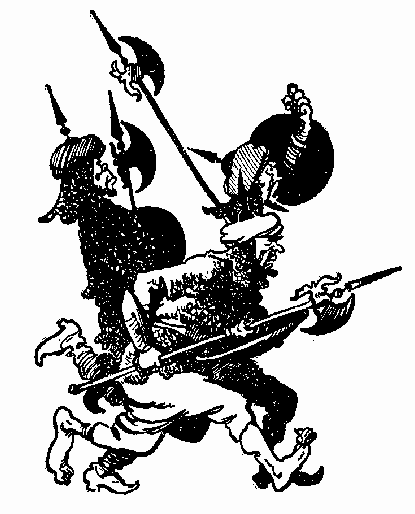
\includegraphics[scale=0.7]{19.png}
\end{figure}

—~О~прохожий, я~тебе расскажу все, если ты~пообещаешь, выслушав, удалиться и~не~тревожить больше мой покой. Этот мешок принадлежит одному арабу, живущему у~нас в~Бухаре, и~обладает чудесным свойством исцелять болезни и~уродства. Хозяин дает его на~подержание, но~за~большие деньги и~не~всем. Я~был хромым, горбатым и~кривым на~один глаз, и~вот я~надумал жениться, и~отец моей невесты, дабы не~огорчить ее~взора созерцанием моих уродств, повел меня к~этому арабу, и~я~получил на~подержание мешок сроком на~четыре часа, уплатив хозяину шестьсот таньга. А~так как этот мешок проявляет свои целебные свойства только вблизи кладбища, то~я~и~пришел после захода солнца сюда, к~старому Каршинскому кладбищу, вместе с~отцом моей невесты, который, завязав веревку на~мешке, удалился, ибо присутствие постороннего человека может испортить все дело. Араб, хозяин мешка, предупредил меня~— как только я~останусь один, ко~мне подлетят три джина, производя шум и~звон своими медными крыльями. И~джины человеческими голосами спросят меня, где на~кладбище закопаны десять тысяч таньга, на~что я~должен ответить им~следующим таинственным заклинанием: «Тот, кто носит медный щит, тот имеет медный лоб. На~месте сокола сидит филин. О~джины, вы~ищете там, где не~прятали, поцелуйте за~это под хвост моего ишака!» Так оно в~точности и~случилось: явились джины и~спросили меня, где закопаны десять тысяч таньга; услышав мой ответ, джины пришли в~неописуемую ярость и~начали бить меня, а~я, памятуя наставления араба, продолжал кричать: «Тот, кто носит медный щит, тот имеет медный лоб, поцелуйте под хвост моего ишака!» Потом джины подхватили мешок и~понесли куда-то... А~дальше я~ничего уже не~помню, очнулся я~через два часа на~том~же самом месте вполне исцеленный~— мой горб исчез, нога выпрямилась, и~глаз прозрел, в~чем я~убедился, глядя в~дырочку, которую кто-то проделал в~мешке еще до~меня. И~теперь я~досиживаю в~мешке свой срок только потому, что деньги все равно заплачены,~— не~пропадать~же им~зря! Конечно, я~совершил ошибку: надо было сговориться с~каким-нибудь человеком, обладающим теми~же уродствами; мы~взяли~бы мешок пополам, просидели~бы в~нем по~два часа, и~наше исцеление обошлось~бы нам всего по~триста таньга. Но~сделанного не~вернешь: пусть пропадают мои деньги, самое главное, что я~все-таки исцелился. Теперь, прохожий, ты~знаешь все, сдержи свое обещание и~удались. Я~немного ослаб после исцеления, мне трудно разговаривать. Уже десятый человек пристает ко~мне с~расспросами, я~устал повторять всем одно и~то~же.

Ростовщик слушал с~глубоким вниманием, прерывая иногда рассказ Ходжи Насреддина возгласами удивления.

\begin{figure}[t]
\centering
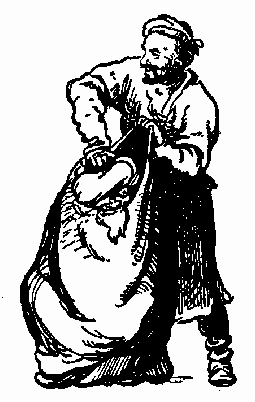
\includegraphics[scale=0.75]{20.png}
\end{figure}

—~Послушай, о~человек, сидящий в~мешке! —~сказал ростовщик. —~Мы~оба можем извлечь пользу из~нашей встречи. Ты~сожалеешь о~том, что не~сговорился заранее с~каким-нибудь человеком, обладающим такими~же уродствами, чтобы взять мешок на~подержание пополам. Но~тебе еще не~поздно сговориться, ибо я~и~есть как раз тот человек, который тебе нужен: я~горбат, хром на~правую ногу и~крив на~один глаз. И~я~охотно уплачу триста таньга за~то, чтобы просидеть в~мешке оставшиеся два часа.

—~Ты, наверное, смеешься надо мной,~— ответил Ходжа Насреддин. —~Может~ли быть такое чудесное совпадение! Если ты~говоришь правду, то~возблагодари аллаха за~ниспослание тебе столь счастливого случая! Я~согласен, прохожий, но~предупреждаю, что я~уплатил вперед и~тебе тоже придется уплатить вперед. В~долг я~не~поверю.

—~Я~уплачу вперед,~— сказал ростовщик, развязывая веревку. —~Не~будем терять времени, ибо минуты идут, а~теперь они принадлежат уже мне.

Вылезая из~мешка. Ходжа Насреддин прикрыл рукавом халата лицо. Но~ростовщику некогда было разглядывать: он~торопливо считал деньги, сожалея о~пролетающих минутах.

С~кряхтением и~стонами он~залез в~мешок, пригнул голову.

Ходжа Насреддин затянул веревку, отбежал и~притаился в~тени за~деревом.

Он~успел как раз вовремя. Со~стороны кладбища послышалась громкая ругань стражников. Сначала из~пролома в~кладбищенском заборе выползли на~дорогу их~длинные тени, затем и~сами они показались, отражая луну медью своих щитов.


\chapter{}

—~Эй~ты, бродяга! —~кричали стражники, толкая мешок ногами, причем оружие их~лязгало и~звенело, что вполне могло сойти за~шум, производимый медными крыльями. —~Мы~обшарили все кладбище и~ничего не~нашли. Говори, о~сын греха, где закопаны десять тысяч таньга?

Ростовщик твердо помнил таинственное заклинание.

—~Тот, кто носит медный щит, тот имеет медный лоб,~— ответил он~из~мешка. —~На~месте сокола сидит филин. О~джины, вы~ищете там, где не~прятали, поцелуйте за~это под хвост моего ишака!

Услышав такие слова, стражники пришли в~неописуемую ярость.

—~Ты~обманул нас, подобный зловонному псу, и~ты~еще называешь нас дураками!\footnote{Арабское слово «джин» означает «злой дух». В~узбекском языке имеется слово «джины», означающее буквально «одержимый злым духом». Употребляется в~смысле бесноватый, сумасшедший, помешанный, полоумный~и, наконец, просто дурак. (Примеч. автора.)} Смотрите, смотрите, он~извалял в~пыли весь мешок, значит, он~катался и~кувыркался по~дороге в~надежде освободиться, пока~мы, раздирая в~кровь руки, трудились на~кладбище! Ты~жестоко поплатишься за~свой обман, о~гнусное порождение лисицы!

Они обрушили на~мешок град тяжелых ударов, не~удовольствовавшись этим, они поочередно сплясали на~мешке в~своих подкованных сапогах. А~ростовщик, следуя наставлениям Ходжи Насреддина, беспрерывно кричал: «Кто носит медный щит, тот имеет медный лоб!..»~— чем довел стражников до~полного исступления. Жалея, что им~не~дозволено самим расправиться с~преступником, они подхватили мешок и~потащили к~водоему.

Ходжа Насреддин вышел из~своего укрытия на~дорогу, обмыл в~арыке лицо, сбросил халат, открыв ночному ветру широкую грудь. Как радостно и~легко было ему сейчас, когда черное дыхание смерти пронеслось, не~опалив его! Он~отошел в~сторону, расстелил халат, подложил камень под голову и~лег,~— он~устал в~душном и~тесном мешке, он~хотел отдохнуть. В~густых вершинах шумел ветер, плыли в~небесном океане золотые сонмы звезд, журчала вода в~арыке; все это было Ходже Насреддину в~десять раз милее и~ближе, чем раньше. «Да! В~мире слишком много хорошего, чтобы я~согласился когда-нибудь умереть, если~бы даже мне твердо пообещали рай; ведь там можно взбеситься от~скуки, сидя вечно и~бесконечно под одним и~тем~же деревом, в~окружении одних и~тех~же гурий».

Так он~думал, лежа под звездами на~теплой земле, чутко прислушиваясь к~неумирающей и~никогда не~засыпающей жизни: стучало сердце в~его груди, вскрикивал ночным голосом филин на~кладбище, кто-то тихонько и~осторожно пробирался через кусты наверно, еж; пряно пахла увядающая трава, и~вся ночь была наполнена какой-то затаенной возней, непонятными шорохами, ползанием и~шуршанием. Мир жил и~дышал~— широкий, равно открытый для всех, принимающий с~одинаковым гостеприимством в~свои безграничные просторы и~муравья, и~птицу, и~человека, и~требующий от~них лишь одного~— не~употреблять во~зло оказанного им~привета и~доверия. Хозяин с~позором изгоняет гостя, который за~праздничным столом, воспользовавшись общим весельем, начинает шарить по~карманам других гостей; точно так~же изгонялся из~веселого и~радостного мира гнусный ростовщик, вполне подобный этому вору. Ходжа Насреддин не~испытывал ни~малейшей жалости к~нему, да~и~как можно пожалеть того, кто исчезновением своим облегчит жизнь тысячам и~тысячам других людей! Ходжа Насреддин сожалел лишь о~том, что ростовщик~— не~единственный и~не~последний злодей на~земле; о, если~бы можно было собрать в~один мешок всех эмиров, сановников, мулл и~ростовщиков и~утопить их~сразу в~священном водоеме шейха Ахмеда, чтобы они своим вредоносным дыханием не~сушили весенних цветов на~деревьях, чтобы звоном своих денег, лживыми проповедями и~лязгом мечей не~заглушали они птичьего щебета, чтобы не~мешали они людям наслаждаться красотой мира и~достойно выполнять свое главное дело на~земле~— быть всегда и~во~всем счастливыми!

Тем временем стражники, боясь опоздать, все убыстряли и~убыстряли шаги, наконец~— пустились бегом. Ростовщик, трясясь и~подпрыгивая в~мешке, смирно ждал конца своего необычайного путешествия; он~слышал лязг оружия, шорох камней под ногами стражников и~удивлялся тому, что могучие джины не~поднимаются в~воздух, а~бегут, распустив совком свои медные крылья и~чертя ими по~земле, как делают это молодые петухи, гоняясь за~курами. Но~вот вдали послышался какой-то гул, напоминающий отдаленный рев горного потока, и~ростовщик сначала подумал, что джины затащили его куда-то в~горы, может быть к~своей обители Хан Тенгри~— Вершине Духов. Но~вскоре он~стал различать отдельные голоса и~убедился, что попал в~ночное многолюдное сборище; судя по~шуму, здесь были тысячи людей, как на~базаре, но~с~каких это пор базары в~Бухаре начали торговать по~ночам? Вдруг он~почувствовал, что возносится вверх: ага, значит, джины решили все-таки подняться на~воздух. Откуда мог он~знать, что стражники в~это время всходили по~лестнице на~помост? Взойдя, они сбросили мешок, он~рухнул, доски вздрогнули и~загремели под ним. Ростовщик охнул и~крякнул.

—~Эй~вы, джины! —~не~выдержал~он. —~Если вы~будете так швырять мешок, то~изуродуете меня еще больше, в~то~время как вам надлежит сделать обратное!

В~ответ он~получил яростный пинок:

—~Ты~сейчас найдешь свое исцеление, о~сын греха, на~дне водоема святого Ахмеда.

\begin{figure}[p]
\centering
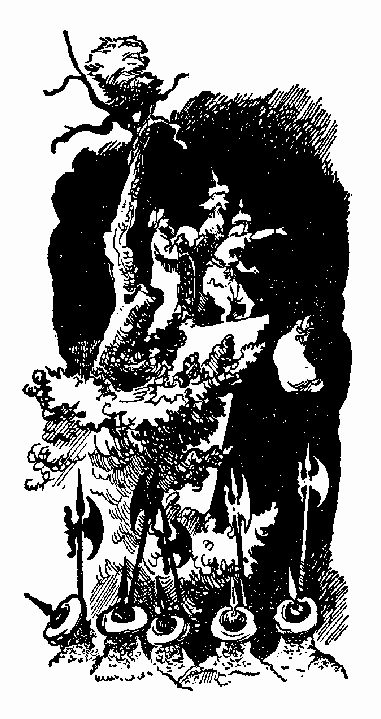
\includegraphics[scale=0.8]{21.png}
\end{figure}

Эти слова привели ростовщика в~полное недоумение: при чем здесь водоем святого Ахмеда? Недоумение ростовщика перешло в~изумление, когда он~услышал над мешком голос своего старинного приятеля (ростовщик мог~бы поклясться в~этом!), почтенного Арсланбека, начальника дворцовой стражи и~войска. Мысли в~голове ростовщика пошли кувырком: откуда взялся вдруг Арсланбек, почему ругает он~джинов за~то, что они задержались в~пути, и~почему джины, отвечая ему, трепещут от~страха и~раболепия; ведь не~может быть, чтобы Арсланбек занимал одновременно должность главного джина! И~как следует теперь поступить~— промолчать или окликнуть его? Так как на~этот счет ростовщик не~получил никаких наставлений, то~и~решил на~всякий случай промолчать.

Между тем гул толпы усиливался, и~все чаще, громче звучало какое-то слово: казалось, все вокруг~— и~земля, и~воздух, и~ветер~— насыщено этим словом,~— оно гудело, шумело, рокотало~и, замирая, отдавалось вдали. Ростовщик притих, вслушиваясь. И~он~разобрал.

—~Ходжа Насреддин!.. —~гудела толпа тысячами голосов. —~Ходжа Насреддин!.. Ходжа Насреддин!..

Вдруг все затихло, и~в~мертвой тишине ростовщик услышал шипение горящих факелов, шелест ветра, всплески воды. Мурашки побежали по~его уродливой спине, черный ужас начал медленно подползать к~нему, обдавая его своим ледяным, цепенящим дыханием.

Раздался новый голос, и~ростовщик мог~бы поклясться, что голос этот принадлежит великому визирю Бахтияру:

—~Во~имя аллаха всемилостивого и~всемогущего! По~повелению великого и~солнцеподобного эмира бухарского, предается смерти преступник и~осквернитель веры, возмутитель спокойствия и~сеятель раздоров Ходжа Насреддин через утопление в~мешке!

Чьи-то руки подхватили мешок и~подняли. Тут ростовщик сообразил, что попал в~смертельную ловушку.

—~Подождите! Подождите! —~завопил~он. —~Что вы~хотите делать со~мной! Подождите, я~не~Ходжа Насреддин, я~— ростовщик Джафар! Отпустите меня! Я~ростовщик Джафар, я~не~Ходжа Насреддин! Куда вы~меня потащили, говорят вам~— я~ростовщик Джафар!

Эмир и~свита в~безмолвии внимали его воплям. Багдадский мудрец Гуссейн Гуслия, сидевший ближе всех к~эмиру, сказал, сокрушенно покачивая головой:

—~Какая бездна бесстыдства сокрыта в~этом преступнике. То~он~называл себя Гуссейном Гуслия, мудрецом из~Багдада, теперь он~пытается обмануть нас, называя себя ростовщиком Джафаром!

—~И~он~думает, что здесь найдутся дураки, которые поверят ему,~— добавил Арсланбек. —~Послушайте, послушайте, как искусно он~подделывает свой голос!

—~Отпустите меня! Я~— не~Ходжа Насреддин, я~— Джафар! —~надрывался ростовщик, в~то~время как два стражника, стоя на~краю помоста, мерными движениями раскачивали мешок, готовясь швырнуть его в~темную воду. —~Я~не~Ходжа Насреддин, сколько раз надо вам повторять!

Но~в~этот миг Арсланбек махнул рукой, и~мешок, грузно переворачиваясь в~воздухе, полетел вниз; раздался сильный всплеск, блеснули в~красном свете факелов брызги, и~вода тяжело сомкнулась, поглотив грешное тело и~грешную душу ростовщика Джафара...

Над толпой в~темноте поднялся и~повис единый огромный вздох. Несколько мгновений стояла страшная тишина, и~вдруг всех потряс пронзительный вопль, полный невыразимой муки.

То~кричала и~билась на~руках своего старого отца прекрасная Гюльджан.

Чайханщик Али отвернулся, обхватил руками голову. Кузнец Юсуп весь дрожал мелкой прерывистой дрожью...


\chapter{}

По~свершении казни эмир со~своей свитой отбыл во~дворец.

Арсланбек, опасаясь, что преступника могут вытащить раньше, чем он~задохнется, приказал оцепить водоем и~не~подпускать никого. Толпа всколыхнулась, отступила под напором стражников и~остановилась, слитно чернея живой молчаливой громадой. Арсланбек попытался разогнать толпу, но~люди только переходили с~одного места на~другое или прятались в~темноту, чтобы, переждав, вернуться на~старое место.

Во~дворце началось великое ликование. Эмир праздновал победу над своим врагом. Сверкало золото и~серебро, кипели котлы, дымили жаровни, гудели бубны, ревели трубы, грохотали, сотрясая воздух, барабаны, и~столько огней было на~этом празднике, что над эмирским дворцом стояло зарево, как от~пожара.

Но~город вокруг дворца молчал, погруженный во~тьму и~объятый скорбной тишиной.

Эмир щедро раздавал подарки, многие в~этот день поживились. Поэты охрипли от~беспрерывного славословия, спины их~начали тихонько, но~сладостно ныть,~— столь часто приходилось нагибаться за~серебряными и~золотыми монетами.

—~Позвать сюда писца! —~приказал эмир; прибежал писец и~быстро заскрипел тростниковым пером.

—~«От~Великого и~Блистательного и~Затмевающего солнце Властителя, Повелителя и~Законодателя Бухары Эмира Бухарского~— Великому и~Блистательному и~Затмевающему солнце Властителю, Повелителю и~Законодателю Хивы Хану Хивинскому посылаются розы привета и~лилии доброжелательства. Сообщаем Вам, о~Возлюбленный и~Царственный Брат Наш, некую новость, которая может согреть огнем восторга Ваше Сердце и~сладостно размягчить Вашу Печень, а~именно: сегодня, в~семнадцатый день месяца Сафара, Мы, Великий Эмир Бухарский, предали всенародной казни известного всему свету своими богохульными и~непотребными деяниями преступника Ходжу Насреддина, да~проклянет его аллах, через утопление в~мешке, каковое утопление совершено было в~Нашем присутствии и~на~Наших Глазах, благодаря чему Мы~Сами царственным словом Нашим свидетельствуем перед Вами, что вышеназванный злодей, возмутитель спокойствия, осквернитель веры. и~сеятель раздоров, ныне не~пребывает в~живых и~не~сможет больше докучать Вам, о~Возлюбленный Брат Наш, своими богомерзкими проделками...»

Такие~же письма эмир написал калифу багдадскому, султану турецкому, шаху иранскому, хану кокандскому, эмиру афганскому и~многим другим государям сопредельных и~несопредельных стран. Великий визирь Бахтияр свернул письма в~трубки, привесил печати и~вручил гонцам, приказав отправляться немедленно. И~в~ночной час открылись, громко скрипя и~визжа петлями, все одиннадцать ворот Бухары, и, разбрызгивая звонкий щебень, высекая искры подковами своих коней, во~все стороны по~большим дорогам помчались гонцы~— в~Хиву, в~Тегеран, в~Стамбул, в~Багдад, в~Кабул и~во~многие другие города.

...Поздней ночью, через четыре часа после казни, Арсланбек увел стражу от~водоема.

—~Кто~бы он~ни~был, хотя~бы сам шайтан, но~он~не~мог остаться живым, пролежав четыре часа в~воде! —~сказал Арсланбек. —~И~не~доставайте его, пусть кто хочет возится с~его поганым трупом.

Как только последний стражник исчез в~темноте~— толпа хлынула к~берегу, зашумела и~загудела; зажглись факелы, которые были приготовлены заранее и~лежали неподалеку в~кустах. Скорбно закричали женщины, оплакивая Ходжу Насреддина.

—~Надо похоронить его как доброго мусульманина,~— сказал старый Нияз.

Гюльджан стояла рядом с~ним, опираясь на~его плечо; она была недвижима и~безмолвна.

Чайханщик Али и~кузнец Юсуп полезли с~баграми в~воду. Они шарили долго, наконец~— зацепили мешок и~поволокли к~берегу. Когда он~показался из~воды~— черный, отблескивающий при свете факелов и~опутанный цепкими водорослями,~— женщины завыли еще громче, заглушая своими воплями звуки веселья, доносившиеся из~дворца.

Десятки рук подхватили мешок.

—~Несите за~мной,~— сказал Юсуп, освещая факелами путь.

Мешок положили под раскидистым деревом на~траву. Столпившийся вокруг народ ждал молча.

Юсуп вынул нож, осторожно разрезал мешок по~длине, заглянул в~лицо мертвому и~вдруг отшатнулся, застыл с~выпученными глазами, силясь что-то вымолвить неповинующимся языком.

Чайханщик Али бросился на~помощь к~Юсупу, но~и~с~чайханщиком стряслось то~же; он~вскрикнул и~вдруг повалился на~спину, обратив к~небу свое толстое пузо.

—~Что случилось? —~загудели в~толпе. —~Пустите нас, покажите нам!

Гюльджан, рыдая, стала на~колени, нагнулась к~бездыханному телу, но~кто-то подсунул факел~— и~она отпрянула в~безмерном страхе и~удивлении.

Тут полезли с~факелами со~всех сторон, берег озарился ярко, и~общий могучий вопль потряс тишину ночи:

—~Джафар!

—~Это~— ростовщик Джафар!

—~Это~— не~Ходжа Насреддин!

Было оцепенение, смятение, а~потом люди вдруг заорали, полезли на~плечи друг другу, началась давка и~толкотня: каждый хотел убедиться собственными глазами. С~Гюльджан творилось такое, что старый Нияз поспешил увести ее~подальше от~берега, опасаясь за~ее~рассудок: она плакала и~смеялась, верила и~не~верила, и~порывалась взглянуть еще.

—~Джафар, Джафар! —~неслись ликующие крики, в~которых бесследно тонул далекий гул веселья во~дворце. —~Это ростовщик Джафар! Это он! И~его сумка с~долговыми расписками здесь!

Прошло много времени, прежде чем кто-то опомнился и~спросил, обращая свой вопрос ко~всем:

—~Но~где~же тогда Ходжа Насреддин? По~всей толпе загудело из~края в~край, из~конца в~конец:

—~Но~где~же тогда Ходжа Насреддин? Куда он~девался, наш Ходжа Насреддин?

—~Здесь~он, здесь! —~раздался знакомый, спокойный голос, и~все, повернувшись, с~изумлением увидели живого и~не~сопровождаемого стражниками Ходжу Насреддина, который шел зевая и~лениво потягиваясь: он~незаметно уснул около кладбища и~поэтому опоздал к~водоему.

—~Я~здесь! —~повторил~он. —~Кому я~нужен, подходите! О~благородные жители Бухары, зачем вы~собрались у~водоема и~что вы~здесь делаете в~такой поздний час?

—~Как зачем собрались? —~ответили сотни голосов. —~Мы~собрались, о~Ходжа Насреддин, чтобы проститься с~тобой, достойно оплакать и~похоронить тебя.

—~Меня? —~сказал~он. —~Оплакивать?.. О~благородные жители Бухары, вы~плохо знаете Ходжу Насреддина, если думаете, что он~собирается когда-нибудь умереть! Я~просто прилег отдохнуть около кладбища, а~вы~уже решили, что я~умер!

Больше ему не~удалось ничего сказать, потому что налетел, крича, толстый чайханщик Али, за~ним~— кузнец Юсуп; Ходжа Насреддин едва не~задохнулся в~их~жарких объятиях. Мелко семеня, подбежал Нияз, но~старика сейчас~же оттеснили. Ходжа Насреддин очутился в~середине большой толпы, каждый хотел обнять его и~поздороваться с~ним, а~он, переходя из~объятий в~объятья, стремился туда, где слышался сердитый и~нетерпеливый голос Гюльджан, которая тщетно старалась пробиться к~нему сквозь толпу. Когда наконец они встретились, Гюльджан повисла на~его шее. Ходжа Насреддин при всех целовал~ее, откинув покрывало, и~никто, даже самые ревностные блюстители законов и~приличий, не~посмел усмотреть в~этом что-либо предосудительное.

Ходжа Насреддин поднял руку, призывая к~тишине и~вниманию.

—~Вы~собрались оплакивать меня, о~жители Благородной Бухары! Да~разве не~знаете~вы, что я~— бессмертен!

\begin{verse}
Я~— Ходжа Насреддин, сам себе господин, \\
И~скажу~— не~совру~— никогда не~умру.	
\end{verse}

Он~стоял, озаренный ярким пламенем шипящих факелов; толпа дружно подхватила его песню, и~над ночной Бухарой понеслось, гудя, звеня и~ликуя:

\begin{verse}
Нищий, босый и~голый, я~— бродяга веселый, \\
Буду жить, буду петь и~на~солнце глядеть!
\end{verse}

Куда было дворцу до~такого веселья и~ликования.

—~Расскажи! —~закричал кто-то. —~Расскажи, как ты~ухитрился утопить вместо себя ростовщика Джафара?

—~Да! —~вспомнил Ходжа Насреддин. —~Юсуп! Ты~помнишь мою клятву?

—~Помню! —~отозвался Юсуп. —~Ты~сдержал~ее, Ходжа Насреддин!

—~Где он? —~спросил Ходжа Насреддин. —~Где ростовщик? Вы~взяли его сумку?

—~Нет. Мы~не~притрагивались к~нему.

—~Ай-ай-ай! —~укоризненно сказал Ходжа Насреддин. —~Неужели вы~не~понимаете, о~жители Бухары, с~избытком наделенные благородством, но~чуточку обиженные умом, что если эта сумка попадет в~руки наследникам ростовщика, то~они выжмут из~вас все долги до~последнего гроша! Подайте мне его сумку!

Десятки людей, крича и~толпясь, бросились выполнять приказание Ходжи Насреддина, принесли мокрую сумку и~подали ему.

Он~наугад вынул одну расписку.

—~Седельник Мамед! —~крикнул~он. —~Кто здесь седельник Мамед?

—~Я,~— ответил тонкий, дребезжащий голос; из~толпы выступил вперед маленький старик в~цветистом, донельзя рваном халате и~с~бороденкой в~три волоса.

—~Завтра~ты, седельник Мамед, должен уплатить по~этой расписке пятьсот таньга. Но~я. Ходжа Насреддин, освобождаю тебя от~уплаты долга; обрати эти деньги на~свои нужды и~купи себе новый халат, ибо твой больше похож на~созревшее хлопковое поле; отовсюду лезет вата!

С~этими словами он~порвал расписку в~клочки. Так он~поступил со~всеми расписками. Когда была порвана последняя. Ходжа Насреддин, сильно размахнувшись, швырнул сумку в~воду.

—~Пусть она лежит на~дне всегда и~вечно, эта сумка! —~воскликнул~он. —~И~пусть никогда никто не~наденет ее~на~себя! О~благородные жители Бухары, нет большего позора для человека, чем носить такую сумку, и~что~бы ни~случилось с~каждым из~вас, и~если даже кто-нибудь из~вас разбогатеет,~— на~что, впрочем, мало надежды, пока здравствуют наш солнцеподобный эмир и~его неусыпные визири,~— но~если так случится и~кто-нибудь из~вас разбогатеет, то~он~никогда не~должен надевать такую сумку, дабы не~покрыть вечным позором и~себя самого, и~свое потомство до~четырнадцатого колена! А~кроме того, он~должен помнить, что на~свете существует Ходжа Насреддин, который шутить не~любит,~— вы~все видели, какому наказанию подверг он~ростовщика Джафара! Теперь я~прощаюсь с~вами, о~жители Благородной Бухары, пришло мне время отправляться в~дальний путь. Гюльджан, ты~поедешь со~мной?!

—~Поеду~— куда хочешь! —~сказала она.

Жители Бухары достойно проводили Ходжу Насреддина. Караван-сарайщики привели для невесты белого, как хлопок, ишака; ни~одного темного пятнышка не~было на~нем, и~он~горделиво сиял, стоя рядом со~своим серым собратом, старинным и~верным спутником Ходжи Насреддина в~скитаниях. Но~серый ишак ничуть не~смущался столь блистательным соседством, спокойно жевал зеленый сочный клевер и~даже отталкивал своей мордой морду белого ишака, как~бы давая этим понять, что, несмотря на~бесспорное превосходство в~масти, белый ишак далеко еще не~имеет перед Ходжой Насреддином таких заслуг, какие имеет~он, серый ишак.

Кузнецы притащили переносный горн и~подковали тут~же обоих ишаков, седельники подарили два богатых седла: отделанное бархатом~— для Ходжи Насреддина и~отделанное серебром~— для Гюльджан. Чайханщики принесли два чайника и~две китайские наилучшие пиалы, оружейник~— саблю знаменитой стали гурда, чтобы Ходже Насреддину было чем обороняться в~пути от~разбойников; коверщики принесли попоны, арканщики~— волосяной аркан, который, будучи растянут кольцом вокруг спящего, предохраняет от~укуса ядовитой змеи, ибо змея, накалываясь на~жесткие волосинки, не~может переползти через него.

Принесли свои подарки ткачи, медники, портные, сапожники; вся Бухара, за~исключением мулл, сановников и~богачей, собирала в~путь своего Ходжу Насреддина.

Гончары стояли в~стороне печальные: им~нечего было подарить. Зачем человеку нужен в~дороге глиняный кувшин, когда есть медный, подаренный чеканщиками?

Но~вдруг возвысил свой голос самый древний из~гончаров, которому насчитывалось уже за~сто лет:

—~Кто это говорит, что~мы, гончары, ничего не~подарили Ходже Насреддину? А~разве его невеста, эта прекрасная девушка, не~происходит из~славного и~знаменитого сословия бухарских гончаров?

Гончары закричали и~зашумели, приведенные в~полное восхищение словами старика. Потом они дали от~себя Гюльджан строгое наставление~— быть Ходже Насреддину верной, преданной подругой, дабы не~уронить славы и~чести сословия.

—~Близится рассвет,~— обратился Ходжа Насреддин к~народу. —~Скоро откроют городские ворота. Мы~с~моей невестой должны уехать незаметно, если~же вы~пойдете нас провожать, то~стражники, вообразив, что все жители Бухары решили покинуть город и~переселиться на~другое место, закроют ворота и~никого не~выпустят. Поэтому~— расходитесь по~домам, о~жители Благородной Бухары, пусть будет спокоен ваш сон, и~пусть никогда не~нависают над вами черные крылья беды, и~пусть дела ваши будут успешны. Ходжа Насреддин прощается с~вами! Надолго~ли? Я~не~знаю и~сам...

На~востоке уже начала протаивать узкая, едва заметная полоска. Над водоемом поднимался легкий пар. Народ начал расходиться, люди гасили факелы, кричали, прощаясь:

—~Добрый путь. Ходжа Насреддин! Не~забывай свою родную Бухару!

Особенно трогательным было прощание с~кузнецом Юсупом и~чайханщиком Али. Толстый чайханщик не~мог удержаться от~слез, которые обильно увлажнили его красные полные щеки.

До~открытия ворот Ходжа Насреддин пробыл в~доме Нияза, но~как только первый муэдзин протянул над городом печально звенящую нить своего голоса~— Ходжа Насреддин и~Гюльджан тронулись в~путь. Старик Нияз проводил их~до~угла,~— дальше Ходжа Насреддин не~позволил, и~старик остановился, глядя вслед им~влажными глазами, пока они не~скрылись за~поворотом. Прилетел легкий утренний ветерок и~начал хлопотать на~пыльной дороге, заботливо заметая следы.

Нияз бегом пустился домой, торопливо поднялся на~крышу, откуда было видно далеко за~городскую стену, и, напрягая старые глаза, смахивая непрошеные слезы, долго смотрел на~бурое, сожженное солнцем взгорье, по~которому вилась, уходя за~тридевять земель, серая лента дороги. Он~долго ждал, в~его сердце начала закрадываться тревога: уж~не~попались~ли Ходжа Насреддин и~Гюльджан в~руки стражников? Но~вот, присмотревшись, старик различил вдали два пятна~— серое и~белое: они все удалялись, все уменьшались, потом серое пятно исчезло, слившись со~взгорьем, а~белое виднелось еще долго, то~пропадая в~лощинах и~впадинах, то~показываясь опять. Наконец и~оно исчезло, растворилось в~поднимающемся мареве. Начинался день, и~начинался зной. А~старик, не~замечая зноя, сидел на~крыше в~горькой задумчивости, его седая голова тряслась, и~душный комок стоял в~горле. Он~не~роптал на~Ходжу Насреддина и~свою дочку, он~желал им~долгого счастья, но~ему было горько и~больно думать о~себе,~— теперь совсем опустел его дом, и~некому скрасить звонкой песней и~веселым смехом его одинокую старость. Подул жаркий ветер, всколыхнул листву виноградника, взвихрил пыль, задел крылом горшки, что сушились на~крыше, и~они зазвенели жалобно, тонко, протяжно, словно~бы и~они грустили о~покинувших дом...

Нияз очнулся, услышав какой-то шум за~спиной, оглянулся: к~нему на~крышу поднимались по~лестнице один за~другим три брата, все~— молодец к~молодцу, и~все~— гончары. Они подошли и~склонились перед стариком в~поклонах, преисполненные глубочайшего уважения.

—~О~почтенный Нияз! —~сказал старший из~них. —~Твоя дочка ушла от~тебя за~Ходжой Насреддином, но~ты~не~должен горевать и~роптать, ибо таков вечный закон земли, что зайчиха не~живет без зайца, лань не~живет без оленя, корова не~живет без быка и~утка не~живет без селезня. А~разве девушка может прожить без верного и~преданного друга, и~разве не~парами сотворил аллах все живущее на~земле, разделив даже хлопковые побеги на~мужские и~женские. Но, чтобы не~была черной твоя старость, о~почтенный Нияз, решили мы~все трое сказать тебе следующее: тот, кто породнился с~Ходжой Насреддином, тот породнился со~всеми жителями Бухары, и~ты, о~Нияз, породнился отныне с~нами. Тебе известно, что прошлой осенью~мы, скорбя и~стеная, похоронили нашего отца и~твоего друга, почтеннейшего Усмана Али, и~ныне у~нашего очага пустует место, предназначенное для старшего, и~мы~лишены ежедневного счастья почтительно созерцать белую бороду, без которой, как равно и~без младенческого крика, дом считается наполовину пустым, ибо хорошо и~спокойно бывает на~душе у~человека только тогда, когда он~находится посередине между тем, обладающим бородою, кто дал ему жизнь, и~между тем, лежащим в~колыбели, которому он~сам дал жизнь. И~поэтому, о~почтенный Нияз, мы~просим тебя преклонить слух к~нашим словам, и~не~отвергать нашей просьбы, и~войти в~наш дом, занять у~нашего очага место, предназначенное для старшего, и~быть нам всем троим за~отца, а~нашим детям за~дедушку.

Братья просили так настойчиво, что Нияз не~мог отказаться: он~вошел к~ним в~дом и~был принят с~великим почтением. Так на~старости лет он~за~свою честную и~чистую жизнь был вознагражден самой большой наградой, какая только существует на~земле для мусульманина: он~стал Нияз-бобо, то~есть дедушка, глава большой семьи, в~которой у~него было четырнадцать внуков, и~взор его мог наслаждаться беспрерывно, переходя с~одних розовых щек, измазанных тутовником и~виноградом, на~другие, не~менее грязные. И~слух его с~тех пор никогда не~был удручаем тишиною, так что ему с~непривычки приходилось даже иной раз тяжеленько и~он~удалялся в~свой старый дом отдохнуть и~погрустить о~таких близких его сердцу и~таких далеких, ушедших неизвестно куда... В~базарные дни он~отправлялся на~площадь и~расспрашивал караванщиков, прибывших в~Бухару со~всех концов земли: не~встретились~ли им~по~дороге два путника~— мужчина, под которым серый ишак, и~женщина на~белом ишаке без единого темного пятнышка? Караванщики морщили свои загорелые лбы, отрицательно качали головами: нет, такие люди им~по~дороге не~попадались.

Ходжа Насреддин, как всегда, исчез бесследно, чтобы вдруг объявиться там, где его совсем не~ожидают.


\chapter{...которая могла~бы послужить началом для новой книги}

\begin{quote}
Я~совершил семь путешествий, и~про каждое путешествие есть удивительный рассказ, который смущает умы.
\flushright{\textit{«Тысяча и~одна ночь»}}
\end{quote}

И~он~объявился там, где его совсем не~ожидали. Он~объявился в~Стамбуле.

Это произошло на~третий день по~получении султаном письма от~эмира бухарского. Сотни глашатаев разъезжали по~городам и~селениям Блистательной Порты\footnote{Блистательная Порта~— одно из~принятых ранее в~европейских дипломатических документах, в~литературе название Османской империи (Турция во~главе с~султаном).}, оповещая народ о~смерти Ходжи Насреддина. Обрадованные муллы дважды в~день, утром и~вечером, оглашали в~мечетях эмирское письмо и~возносили благодарность аллаху.

Султан пировал во~дворцовом саду, в~прохладной тени тополей, орошаемых влажной пылью фонтанов. Вокруг теснились визири, мудрецы, поэты и~прочая дворцовая челядь, жадно ожидавшая подачек.

Черные рабы двигались вереницами с~дымящимися подносами, кальянами и~кувшинами в~руках. Султан был в~очень хорошем расположении духа и~беспрерывно шутил.

—~Почему сегодня, несмотря на~такую жару, в~воздухе чувствуется сладостная легкость и~благоухание? —~лукаво прищурившись, спрашивал он~мудрецов и~поэтов. —~Кто из~вас достойно ответит на~наш вопрос?

И~они, кидая умильные взгляды на~кошелек в~его руках, отвечали:

—~Дыхание нашего сиятельного повелителя насытило воздух сладостной легкостью, а~благоухание распространилось потому, что душа нечестивого Ходжи Насреддина перестала наконец источать свой гнусный смрад, отравляющий ранее весь мир.

В~стороне, наблюдая за~порядком, стоял охранитель спокойствия и~благочестия в~Стамбуле~— начальник стражи, отличавшийся от~своего достойного бухарского собрата Арсланбека разве только еще большей свирепостью да~необычайной худобой, каковые качества сопутствовали в~нем друг другу, что было давно замечено жителями Стамбула, и~они еженедельно с~тревогой в~глазах расспрашивали дворцовых банщиков о~состоянии почтенных телес начальника,~— если сведения были зловещими, то~все жители, обитавшие близ дворца, прятались по~домам и~без крайней необходимости не~выходили никуда до~следующего банного дня. Так вот, этот самый приводящий в~трепет начальник стоял в~стороне; его голова, увенчанная чалмой, торчала на~длинной и~тонкой шее, как на~шесте (многие жители Стамбула затаенно вздохнули~бы, услышав такое сравнение!).

Все шло очень хорошо, ничто не~омрачало праздника и~не~предвещало беды. Никто и~не~заметил дворцового надзирателя, который, привычно и~ловко проскользнув между придворными, подошел к~начальнику стражи, что-то шепнул ему. Начальник вздрогнул, переменился в~лице и~торопливыми шагами вышел вслед за~надзирателем. Через минуту он~вернулся~— бледный, с~трясущимися губами. Расталкивая придворных, он~подошел к~султану и~в~поклоне сломался перед ним пополам:

—~О~великий повелитель!..

—~Что там еще? —~недовольно спросил султан. —~Неужели ты~даже в~такой день не~можешь удержать при себе свои палочные и~тюремные новости? Ну, говори скорей!

—~О~сиятельный и~великий султан, язык мой отказывается...

Султан встревожился, сдвинул брови. Начальник стражи полушепотом закончил:

—~Он~— в~Стамбуле!

—~Кто? —~глухо спросил султан, хотя сразу понял, о~ком идет речь.

—~Ходжа Насреддин!

Начальник стражи тихо произнес это имя, но~придворные имеют чуткий слух; по~всему саду зашелестело:

—~Ходжа Насреддин! Он~— в~Стамбуле!.. Ходжа Насреддин в~Стамбуле!

—~Откуда ты~знаешь? —~спросил султан; голос его был хриплым. —~Кто сказал тебе? Возможно~ли это, если мы~имеем письмо эмира бухарского, в~котором он~своим царственным словом заверяет нас, что Ходжа Насреддин больше не~пребывает в~живых.

Начальник стражи подал знак дворцовому надзирателю, и~тот подвел к~султану какого-то человека с~плоским носом на~рябом лице, с~желтыми беспокойными глазами.

—~О~повелитель! —~пояснил начальник стражи. —~Этот человек долго служил шпионом при дворце эмира бухарского и~очень хорошо знает Ходжу Насреддина. Потом этот человек переехал в~Стамбул, и~я~взял его на~должность шпиона, в~каковой должности он~состоит и~сейчас.

—~Ты~видел его? —~перебил султан, обращаясь к~шпиону. —~Ты~видел собственными глазами? Шпион ответил утвердительно.

—~Но~ты, может быть, обознался?

Шпион ответил отрицательно. Нет, он~не~мог обознаться. И~рядом с~Ходжой Насреддином ехала какая-то женщина на~белом ишаке.

—~Почему~же ты~не~схватил его сразу? —~воскликнул султан. —~Почему ты~не~предал его в~руки стражников?

—~О~сиятельный повелитель! —~ответил шпион и~повалился, дрожа, на~колени. —~В~Бухаре я~попал однажды в~руки Ходжи Насреддина, и~если~бы не~милость аллаха, то~не~ушел~бы от~него живым. И~когда я~сегодня увидел его на~улицах Стамбула, то~зрение мое помутилось от~страха, а~когда я~очнулся, то~он~уже исчез.

—~Таковы твои шпионы! —~воскликнул султан, блеснув глазами на~согнувшегося начальника стражи. —~Один только вид преступника приводит их~в~трепет!

Он~оттолкнул ногой рябого шпиона и~удалился в~свои покои, сопровождаемый длинной цепью черных рабов.

Визири, сановники, поэты и~мудрецы тревожно гудящей толпой устремились к~выходу.

Через пять минут в~саду никого не~осталось, кроме начальника стражи, который, глядя в~пустоту остановившимися мутными глазами, бессильно опустился на~мраморный край водоема и~долго сидел, внимая в~одиночестве тихому плеску и~смеху фонтанов. И~казалось, он~в~одно мгновение так похудел и~высох, что если~бы жители Стамбула увидели его, то~бросились~бы врассыпную кто куда, не~подбирая потерянных туфель.

А~рябой шпион в~это время мчался, задыхаясь, по~накаленным улицам к~морю. Там нашел он~арабский корабль, готовый к~отплытию.

Хозяин корабля, нисколько не~сомневаясь в~том, что видит перед собою бежавшего из~тюрьмы разбойника, заломил непомерную цену; шпион не~стал торговаться, вбежал на~палубу и~забился в~темный грязный угол. Потом, когда тонкие минареты Стамбула потонули в~голубой дымке и~свежий ветер надул паруса,~— он~выполз из~своего убежища, обошел корабль, заглянул в~лицо каждому человеку и~наконец успокоился, удостоверившись, что Ходжи Насреддина на~корабле нет.

С~тех пор весь остаток своей жизни рябой шпион прожил в~постоянном и~непрерывном страхе: куда~бы ни~приезжал он~— в~Багдад, в~Каир, в~Тегеран или Дамаск,~— ему не~удавалось прожить спокойно больше трех месяцев, потому что в~городе обязательно появлялся Ходжа Насреддин. И, содрогаясь при мысли о~встрече с~ним, рябой шпион бежал все дальше и~дальше; здесь будет вполне уместно сравнить Ходжу Насреддина с~могучим ураганом, который дыханием своим беспрестанно гонит перед собой сухой желтый лист, выдирает его из~травы и~выдувает его из~расщелин. Так был наказан рябой шпион за~все зло, которое он~причинил людям!..

А~на~другой день в~Стамбуле начались удивительные и~необычайные события!.. Но~не~следует человеку рассказывать о~том, чему он~сам не~был свидетелем, и~описывать страны, которых не~видел; этими словами мы~и~закончим в~нашем повествовании последнюю главу, которая могла~бы послужить началом для новой книги о~дальнейших похождениях несравненного и~бесподобного Ходжи Насреддина в~Стамбуле, Багдаде, Тегеране, Дамаске и~во~многих других прославленных городах...

\end{document}